%%%%%%%%%%%%%%%%%%%%%%%%%%%%%%%%%%%%%%%%%
% Thin Sectioned Essay
% LaTeX Template
% Version 1.0 (3/8/11)
%
% This template has been downloaded from:
% http://www.LaTeXTemplates.com
%
% Original Author:
% Nicolas Diaz (nsdiaz@uc.cl) with extensive modifications by:
% Vel (vel@latextemplates.com)
%
% License:
% CC BY-NC-SA 3.0 (http://creativecommons.org/licenses/by-nc-sa/3.0/)
%
%%%%%%%%%%%%%%%%%%%%%%%%%%%%%%%%%%%%%%%%%

%----------------------------------------------------------------------------------------
%	PACKAGES AND OTHER DOCUMENT CONFIGURATIONS
%----------------------------------------------------------------------------------------

\documentclass[a4paper, 11pt]{article} % Font size (can be 10pt, 11pt or 12pt) and paper size (remove a4paper for US letter paper)

\usepackage[protrusion=true,expansion=true]{microtype} % Better typography
\usepackage{graphicx} % Required for including pictures
\usepackage{wrapfig} % Allows in-line images

\usepackage{mathpazo} % Use the Palatino font
\usepackage[T1]{fontenc} % Required for accented characters
\linespread{1.05} % Change line spacing here, Palatino benefits from a slight increase by default

\makeatletter
\renewcommand\@biblabel[1]{\textbf{#1.}} % Change the square brackets for each bibliography item from '[1]' to '1.'
\renewcommand{\@listI}{\itemsep=0pt} % Reduce the space between items in the itemize and enumerate environments and the bibliography

\renewcommand{\maketitle}{ % Customize the title - do not edit title and author name here, see the TITLE block below
\begin{flushleft} % Right align
{\LARGE\@title} % Increase the font size of the title

\vspace{50pt} % Some vertical space between the title and author name

{\large\@author} % Author name
\\\@date % Date

\vspace{40pt} % Some vertical space between the author block and abstract
\end{flushleft}
}

%----------------------------------------------------------------------------------------
%	TITLE
%----------------------------------------------------------------------------------------

\title{\textbf{NIKA2 research note}\\   
\textsc{NIKA2 Commissioning results v1.0}} % Subtitle


\author{NIKA2 team % Author
\\{\textit{NIKA2 collaboration}}} % Institution

\date{\today} % Date



%----------------------------------------------------------------------------------------

\begin{document}

\maketitle % Print the title section

%----------------------------------------------------------------------------------------
%	ABSTRACT AND KEYWORDS
%----------------------------------------------------------------------------------------

%\renewcommand{\abstractname}{Summary} % Uncomment to change the name of the abstract to something else

\begin{abstract}
This notes describe the main results of the NIKA2 commissioning campaigns.
\end{abstract}

%\hspace*{3,6mm}\textit{Version:}  % Version

\vspace{30pt} % Some vertical space between the abstract and first section

%----------------------------------------------------------------------------------------
%	ESSAY BODY
%----------------------------------------------------------------------------------------

%\tableofcontents

\section{Introduction}

\subsection{Commissioning goals}
The main goal of the NIKA2 commissioning runs described below is to check the performance of the instrument and
its stability with respect to the specifications described in Table \ref{nika2specs}.

%\begin{table}[h]
%\caption{Commissioning campaigns and dates}
%\label{nika2specs}
%\begin{tabular}{|c|c|c|s}
%\hline 
% FWHM &   &  \\
%\hline  
%\hline 
%\end{tabular} 
%\end{table} 



\subsection{Commissioning runs}
We had 9 commissioning runs for NIKA2 as described in Table~\ref{nika2runs}.

%\begin{table}[h]
%\caption{Commissioning campaigns, dates and general comment%
%\label{nika2runs}
%\begin{tabular}{|c|c|c|}
%\hline 
%RUN  &  Dates & General comments \\ 
%\hline 
%N2R1 &      xx  &  xx \\  
 
%\hline 
%\end{tabular} 
%\end{table} 

% ---------------------------------------
\section{Bandpasses}
What actually matters more than the ``central frequency'' that depends on many
assumptions and definitions are the bandpasses. We should make available in a
.fits file, clearly, our bandpasses to avoid future misunderstanding and propagation of
false numbers. Official values should be 150 and 260~GHz. We should also clearly
state that these measured bandpasses were done with the difference of two
black-bodies, hence they include a $\nu^2$ RJ term.\\

With these bandpasses and an official ATM spectrum, we expect an opacity ratio of
XX between 1 and 2mm and see~\ref{se:opacities} for more details.

% ---------------------------------------
\section{sensitivities}

\begin{figure}
\begin{center}
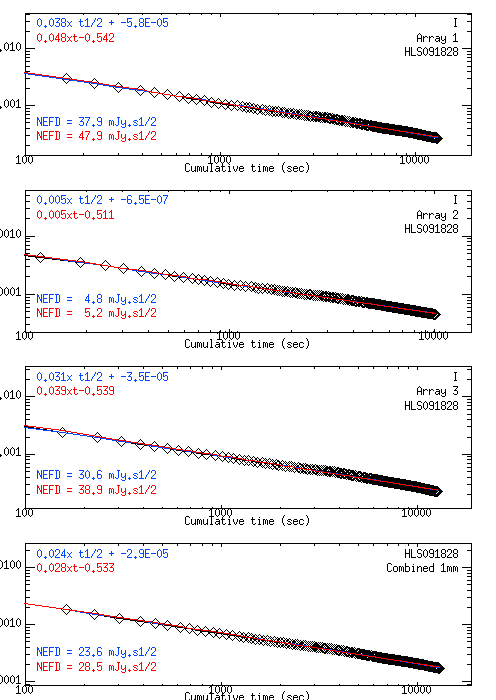
\includegraphics[clip, angle=0, scale = 0.5]{Figures/NEFD_HLS091828_20170226s415_FXDC0C1_GaussPhot.png}
\caption{Kids Xcalib with fixed fwhm 12.5 and 18.5, HLS091828.}
\label{fig:nefd_vs_t}
\end{center}
\end{figure}

{\bf The specs/goals ``NEFD on X \% of pixels'' should be understood as : we have
XX\% valid pixels, and with these pixels, we have an NEFD of YY. We should not
discard some fraction of our pixels and estimate an NEFD on this subset.}\\

HLS091828 is moderately fain source, expected to be below 100~mJy at 1mm and
XX~mJy at 2mm {\bf check values in NIKA1 paper + use SED for predictions in
  NIKA2's bands}. This source was chosen for its flux and its availability during
Run9 for long integration. It has been observed for XX hours in total over three
nights. These data can be used to derive the NEFD in several ways. One is to fit
the evolution of the uncertainty on the flux of the source with the integration
time. Another one is to produced jackknife maps with the data and to measure the
uncertainty on the flux in the end, while estimating the time of
integration. Fig.~\ref{fig:nefd_vs_t} shows the decrease of the uncertainty on
the measured flux at the center of the map as a function of time. We either fit
a power law or fix the power law to -0.5 and fit only the amplitude. Results are
summarized in Tab.~\ref{tab:nefd}


\begin{table}
\begin{tabular}{|l|l|l|}
\hline
Array & Free power law & Fixed power law $t^{-0.5}$\\
\hline
A1 & $47.9$ mJy.s$^{-0.54}$ & $37.9$ mJy.s$^{1/2}$\\
A2 & $5.2$ mJy.s$^{-0.51}$  & $4.8$ mJy.s$^{1/2}$\\
A3 & $38.9$ mJy.s$^{-0.54}$ & $30.6$ mJy.s$^{1/2}$\\
A1 \& A3 & $28.5$ mJy.s$^{-0.53}$ & $23.6$ mJy.s$^{1/2}$\\
\hline
\end{tabular}
\end{table}


% ---------------------------------------
\section{Focal plane reconstruction}
\label{se:fov}

\begin{figure}
\begin{center}
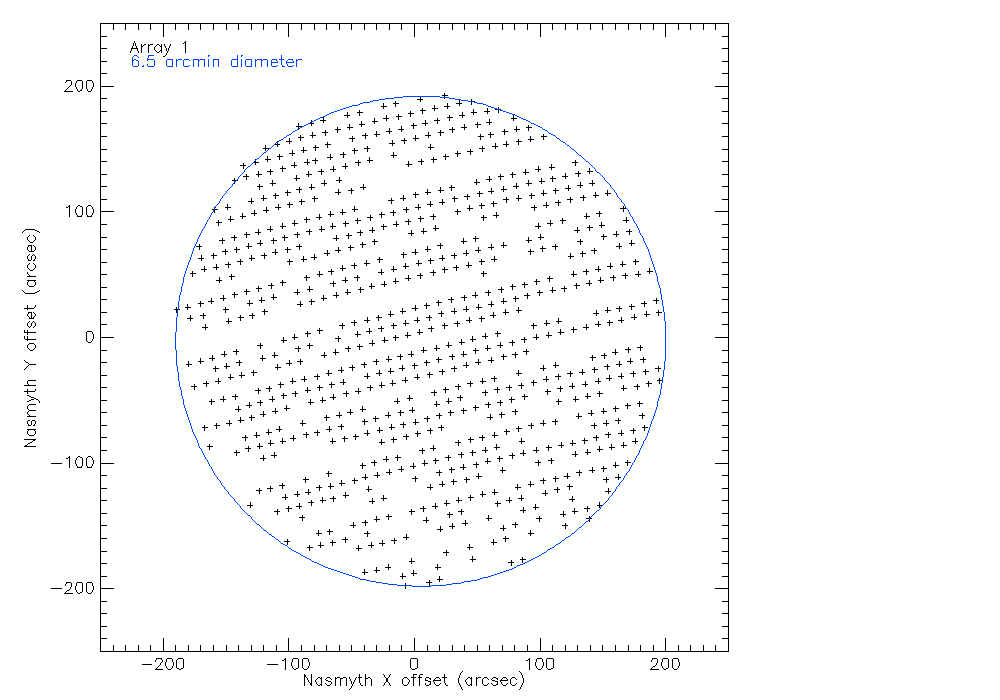
\includegraphics[clip, angle=0, scale = 0.15]{Figures/FOV_A1.png}
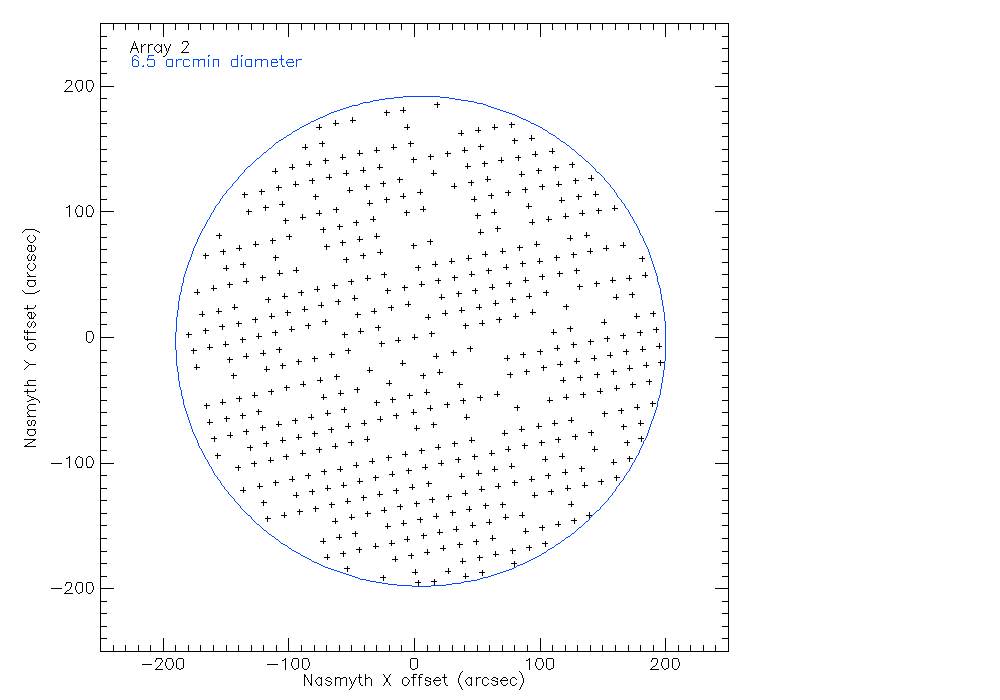
\includegraphics[clip, angle=0, scale = 0.15]{Figures/FOV_A2.png}
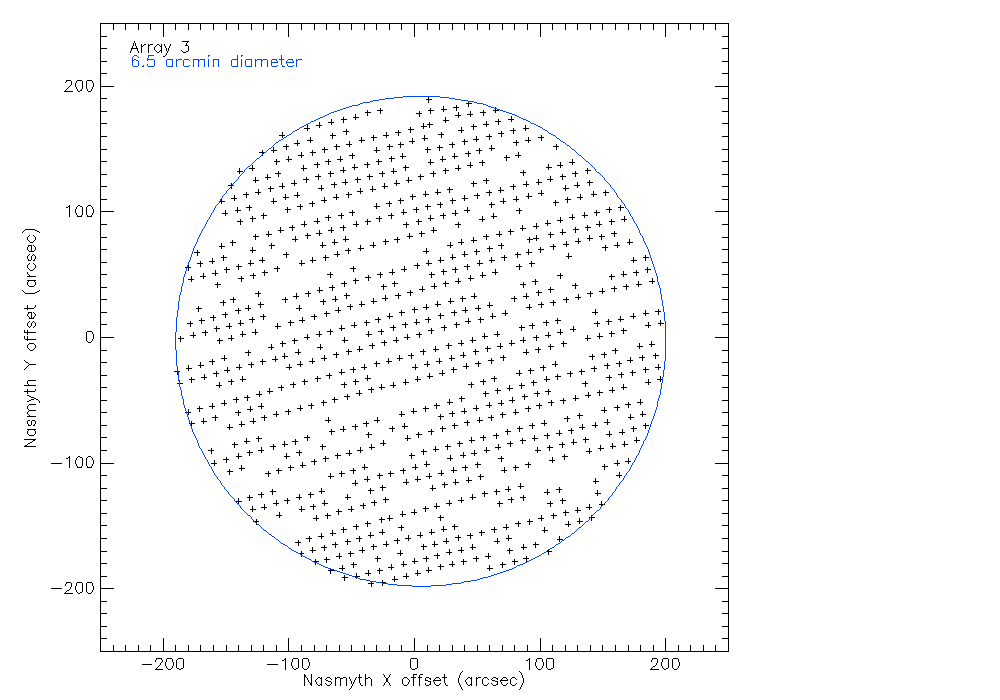
\includegraphics[clip, angle=0, scale = 0.15]{Figures/FOV_A3.png}
\caption{Nasmyth offsets of each array, from beammap 26s415 on 3C84.}
\label{fig:fov}
\end{center}
\end{figure}

\begin{table}
\begin{tabular}{|l|l|l|}
\hline
Array & Number of valid kids & Fraction of all kids\\
\hline
A1 & 793 & 0.75\\
A2 & 481 & 0.83\\
A3 & 872 & 0.83\\
\hline
\end{tabular}
\end{table}

\begin{equation}
FOV diameter = \sqrt{4 N_{tot. kids} * gridstep^2/\pi}
\end{equation}

The same definition applies to ``Effective FOV'' to avoid extra multiplication
by the fraction of valid pixels

\begin{equation}
F\lambda = gridstep\times D(30m)/\lambda
\end{equation}

% ----------------------------------------
\section{Opacity derivation}
\label{se:opacities}


\begin{figure}
\begin{center}
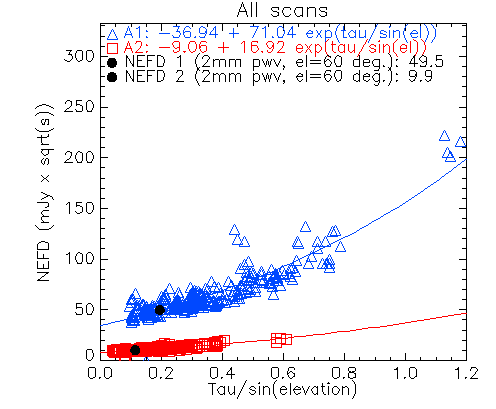
\includegraphics[clip, angle=0, scale =
  0.5]{Figures/NEFD_vs_tau_20170226s415_FXDC0C1_Jy_common_mode_kids_out.png}
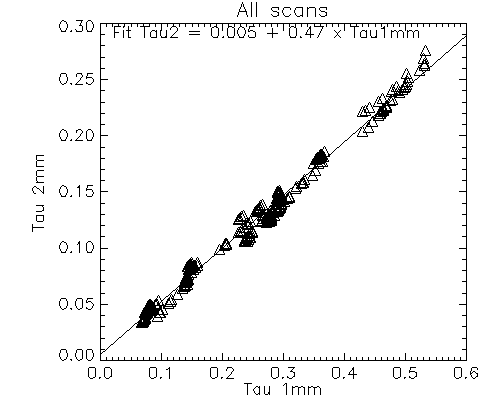
\includegraphics[clip, angle=0, scale =
  0.5]{Figures/tau1_tau2_20170226s415_FXDC0C1_GaussPhot_common_mode_kids_out.png}
\caption{}
\label{fig:fov}
\end{center}
\end{figure}

\begin{figure}
\begin{center}
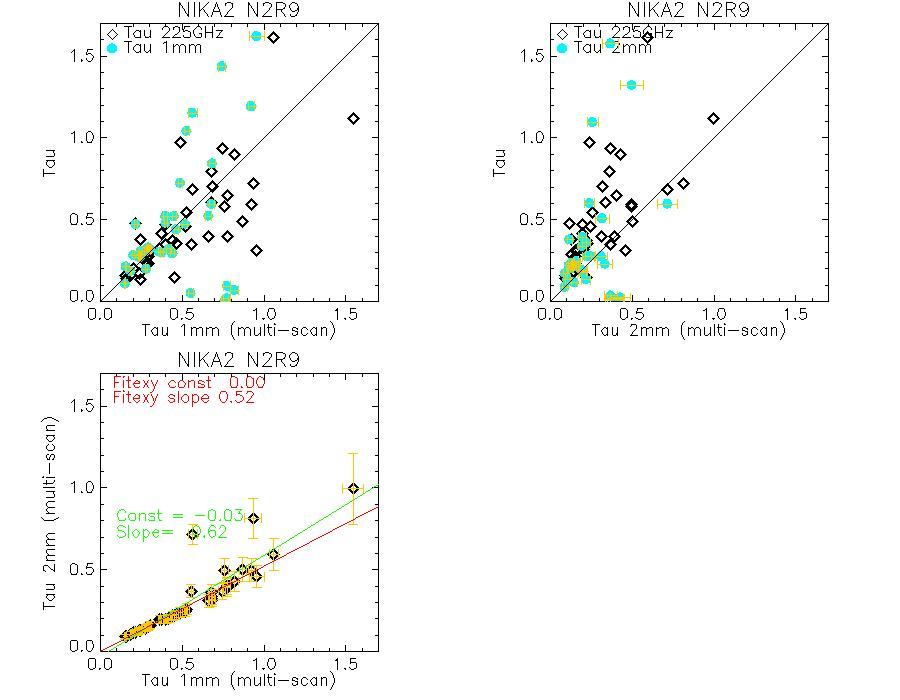
\includegraphics[clip, angle=0, scale = 0.5]{Figures/test_allskd_N2R9.jpg}
\caption{}
\label{fig:fov}
\end{center}
\end{figure}


Note: most of this section is already on the wiki.
\begin{itemize}
\item Description of the method
\item comparison to EMIR
\end{itemize}

%------------------------------------------
\section{Beam pattern}

%------------------------------------------
\section{Calibration}

\begin{figure}
\begin{center}
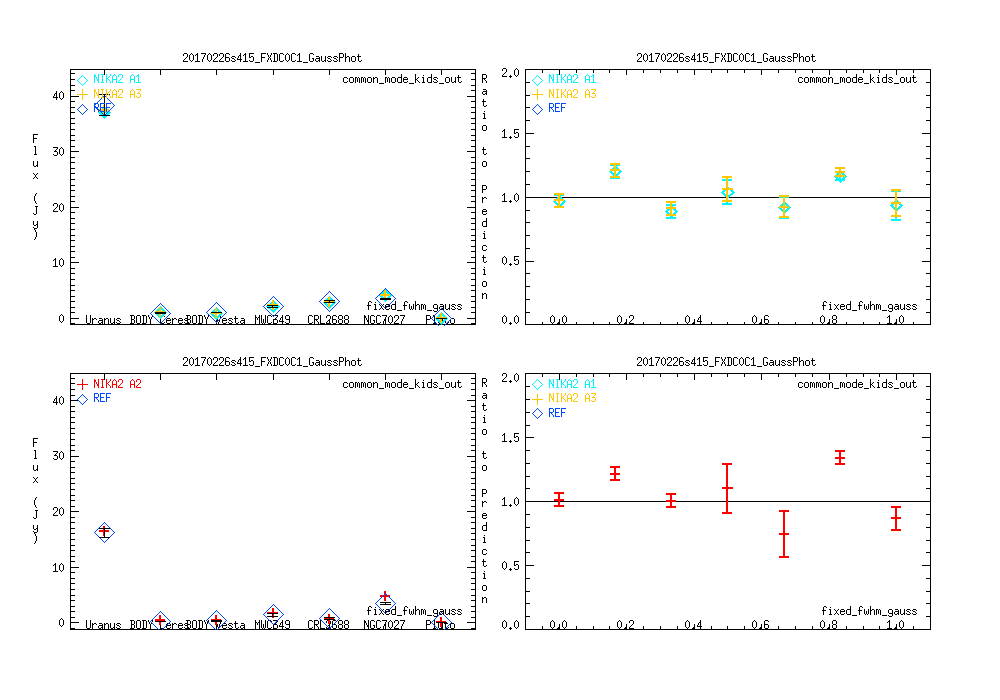
\includegraphics[clip, angle=0, scale = 0.4]{Figures/Calibrators_N2R9_20170226s415_FXDC0C1_GaussPhotFluxType_fixed_fwhm_gauss.png}
\caption{Decorrelation mask: 100 or 60 arcsec, KID cross-calib with fixed fwhm
  (12.5 and 18.5), then absolute photometry with the same fixed fwhm. Note:
  NGC7027 not point like and not corrected for here. Error bars from NIKA2
  measurements and abs. cal. uncertainties by JFL.}
\label{fig:fov}
\end{center}
\end{figure}




%------------------------------------------
\section{Noise description: TOI and maps}

%------------------------------------------
\section{Dark tests}
\section{Detector-Detector correlation matrix}

For this work we have used several decorrelation methods trying to identify possible multiple components in the noise. Notice that in the following the atmospheric signal will be considered simply as correlated sky noise. The main decorrelation methods used are:

\begin{enumerate}
\item[CM] {\bf Common mode decorrelation}. We search for a common mode template using all detectors of the same array. To avoid bias from bad detectors we consider the median common mode.

\item[PCA] {\bf Principal Component Analysis}. For each NIKA2 array independently we decompose the covariance matrix in principal components. From those we derive up to 10 independent templates corresponding to the largest eigenvalue values.

\item[BC] {\bf Best correlated pixels}. For each detector in a given array we identify those detectors which are more correlated to it (a minimum of 14). Using those detectors we compute a common mode as in method CM. 

\item[ALL] {\bf All detectors}. For earch detector of a given array we use all other detectors of the same array as templates and perform a linear fit.

\end{enumerate}

We present in Figure~\ref{corrs299} the detector noise correlation matrices computed for the N2R7 dark scan 20161211s299 for the three arrays (A1, A2, and A3 from left to right). From top to bottom we present the correlation matrices for the raw data (no decorrelation), and for the CM, PCA, and BC decorrelated data. For each array the extent and name (from letter A to T) of the electronic boxes is indicated on the left of the figure. Notice that each electronic box consists of 5 subbands. \\

In the case of the raw data we observe very different structures for the three arrays. In arrays A1 and A2, we observe significant structure going from very correlated detectors to fully uncorrelated ones. This is observed even within a given electronic box or even between detectors from the same electronic subband. By contrast in A3 the detectors seems to be fully correlated. After CM decorrelation we observe that there is still significant correlation and anti-correlation for some detectors. In particular we observe a very clear pattern in A2 for electronic box A. In the case of the PCA decorrelated data the correlation matrix becomes much more diagonal although still shows significant level correlation within electronic subbands. We also notice that using the BC decorrelation improves with respect to the CM decorrelation but it is worse than the PCA case. These results tends indicate various electronic or detector related noise components. \\

In Figure~\ref{corrs72} we show the noise correlation matrices for the N2R7 faint source scan 20161213s72. As expected the raw data noise correlation is dominated by atmospheric noise and we observe full correlation between detectors. After decorrelation the results are very similar to those found for N2R7 dark scan 20161211s299. There is residual significant correlation and anti-correlation after CM decorrelation. PCA decorrelation leads to a more diagonal correlation matrices. For the BC decorrelation the results are worse (more residual correlation and anti-correlation) and close to those of the CM decorrelation. As before there are good indications of multiple electronic-detector noise components. It is interesting to note that the detector-electronic noise correlation patterns seems to be the same for dark tests and for sky data. 

We have repeated the same analysis on scans of the N2R4 both for dark tests, scan 20160504s97, and faint sources, scan 20160313s87. We find few significant differences with respect to previoius results. In the case of the dark test and for the raw data, the A1 and A2 detectors seems to be more correlated. Furthermore A2 show more significant correlation after CM decorrelation for electronic boxes B and D. Array A1 show also significant residual correlation and anti-correlation after CM et BC decorrelations. For the faint source N2R4 scan 
20160313s87 we observe similar behavior but the pattern of the correlation matrices are not the same that for the dark test scan.

\begin{figure}[ht] % Inline image example
\begin{center}
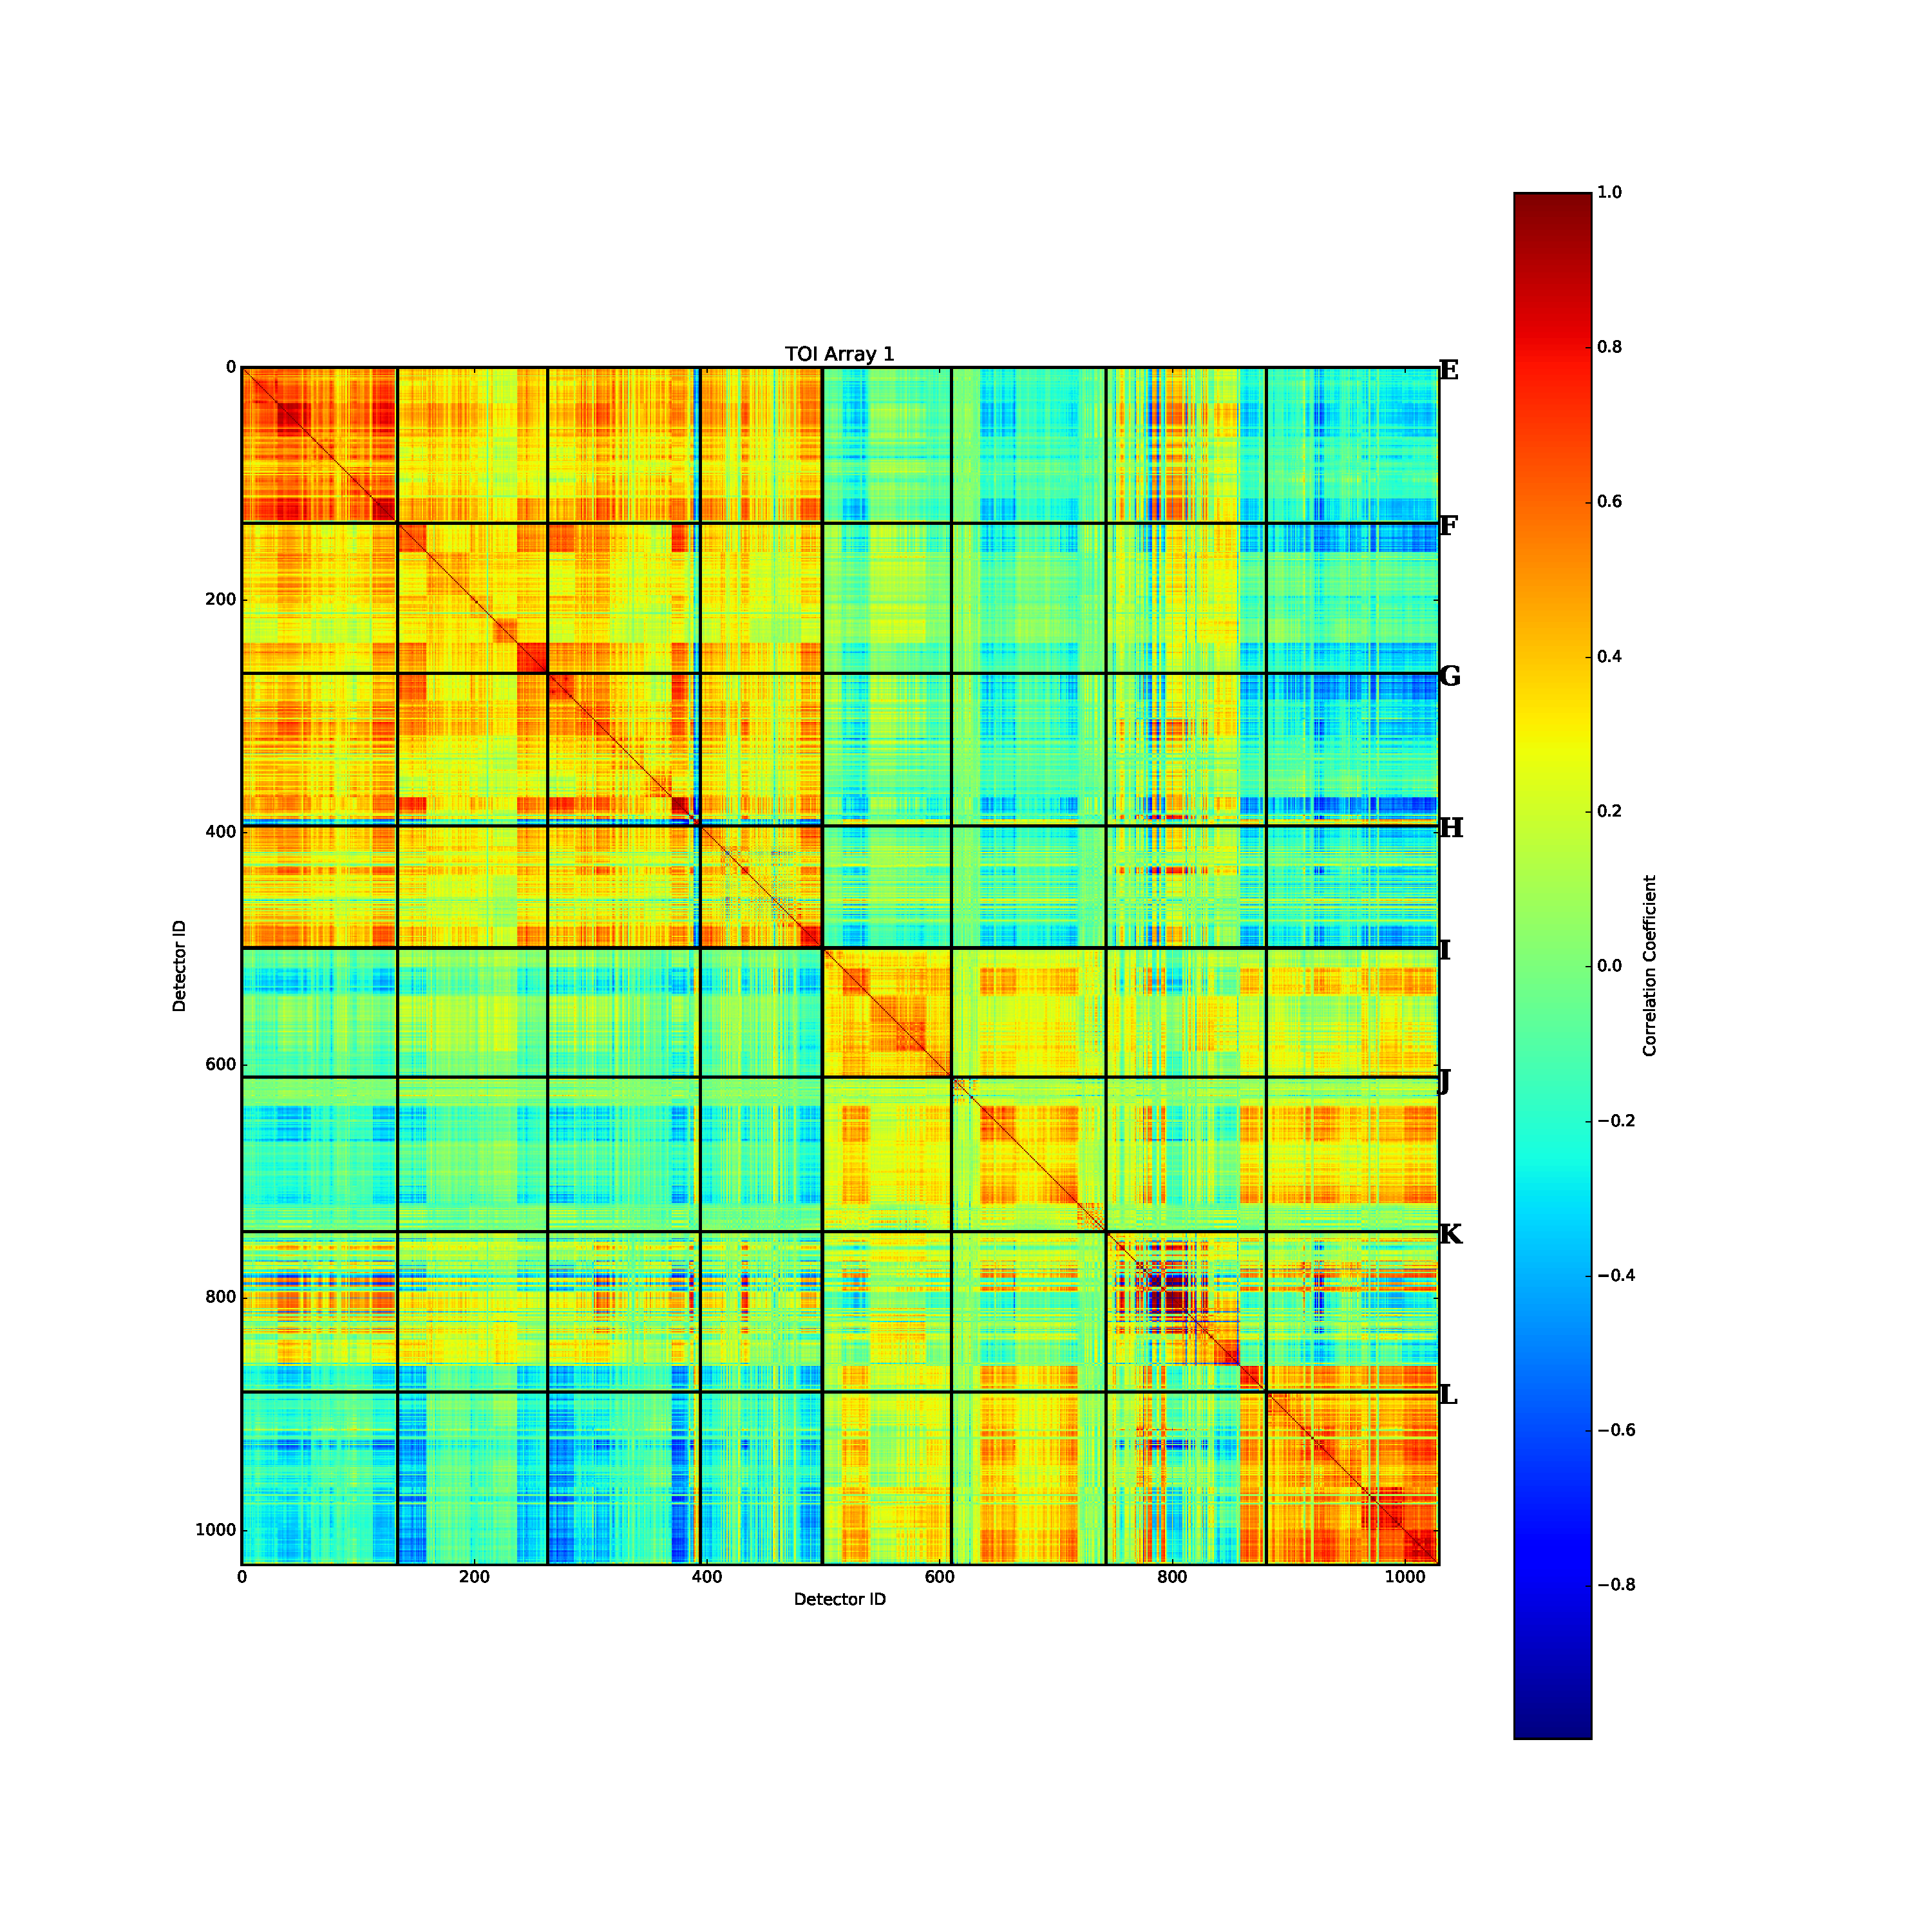
\includegraphics[width=0.3\textwidth]{Figures/DarkTests/corrmat_TOI_array_1_20161211s299.pdf}
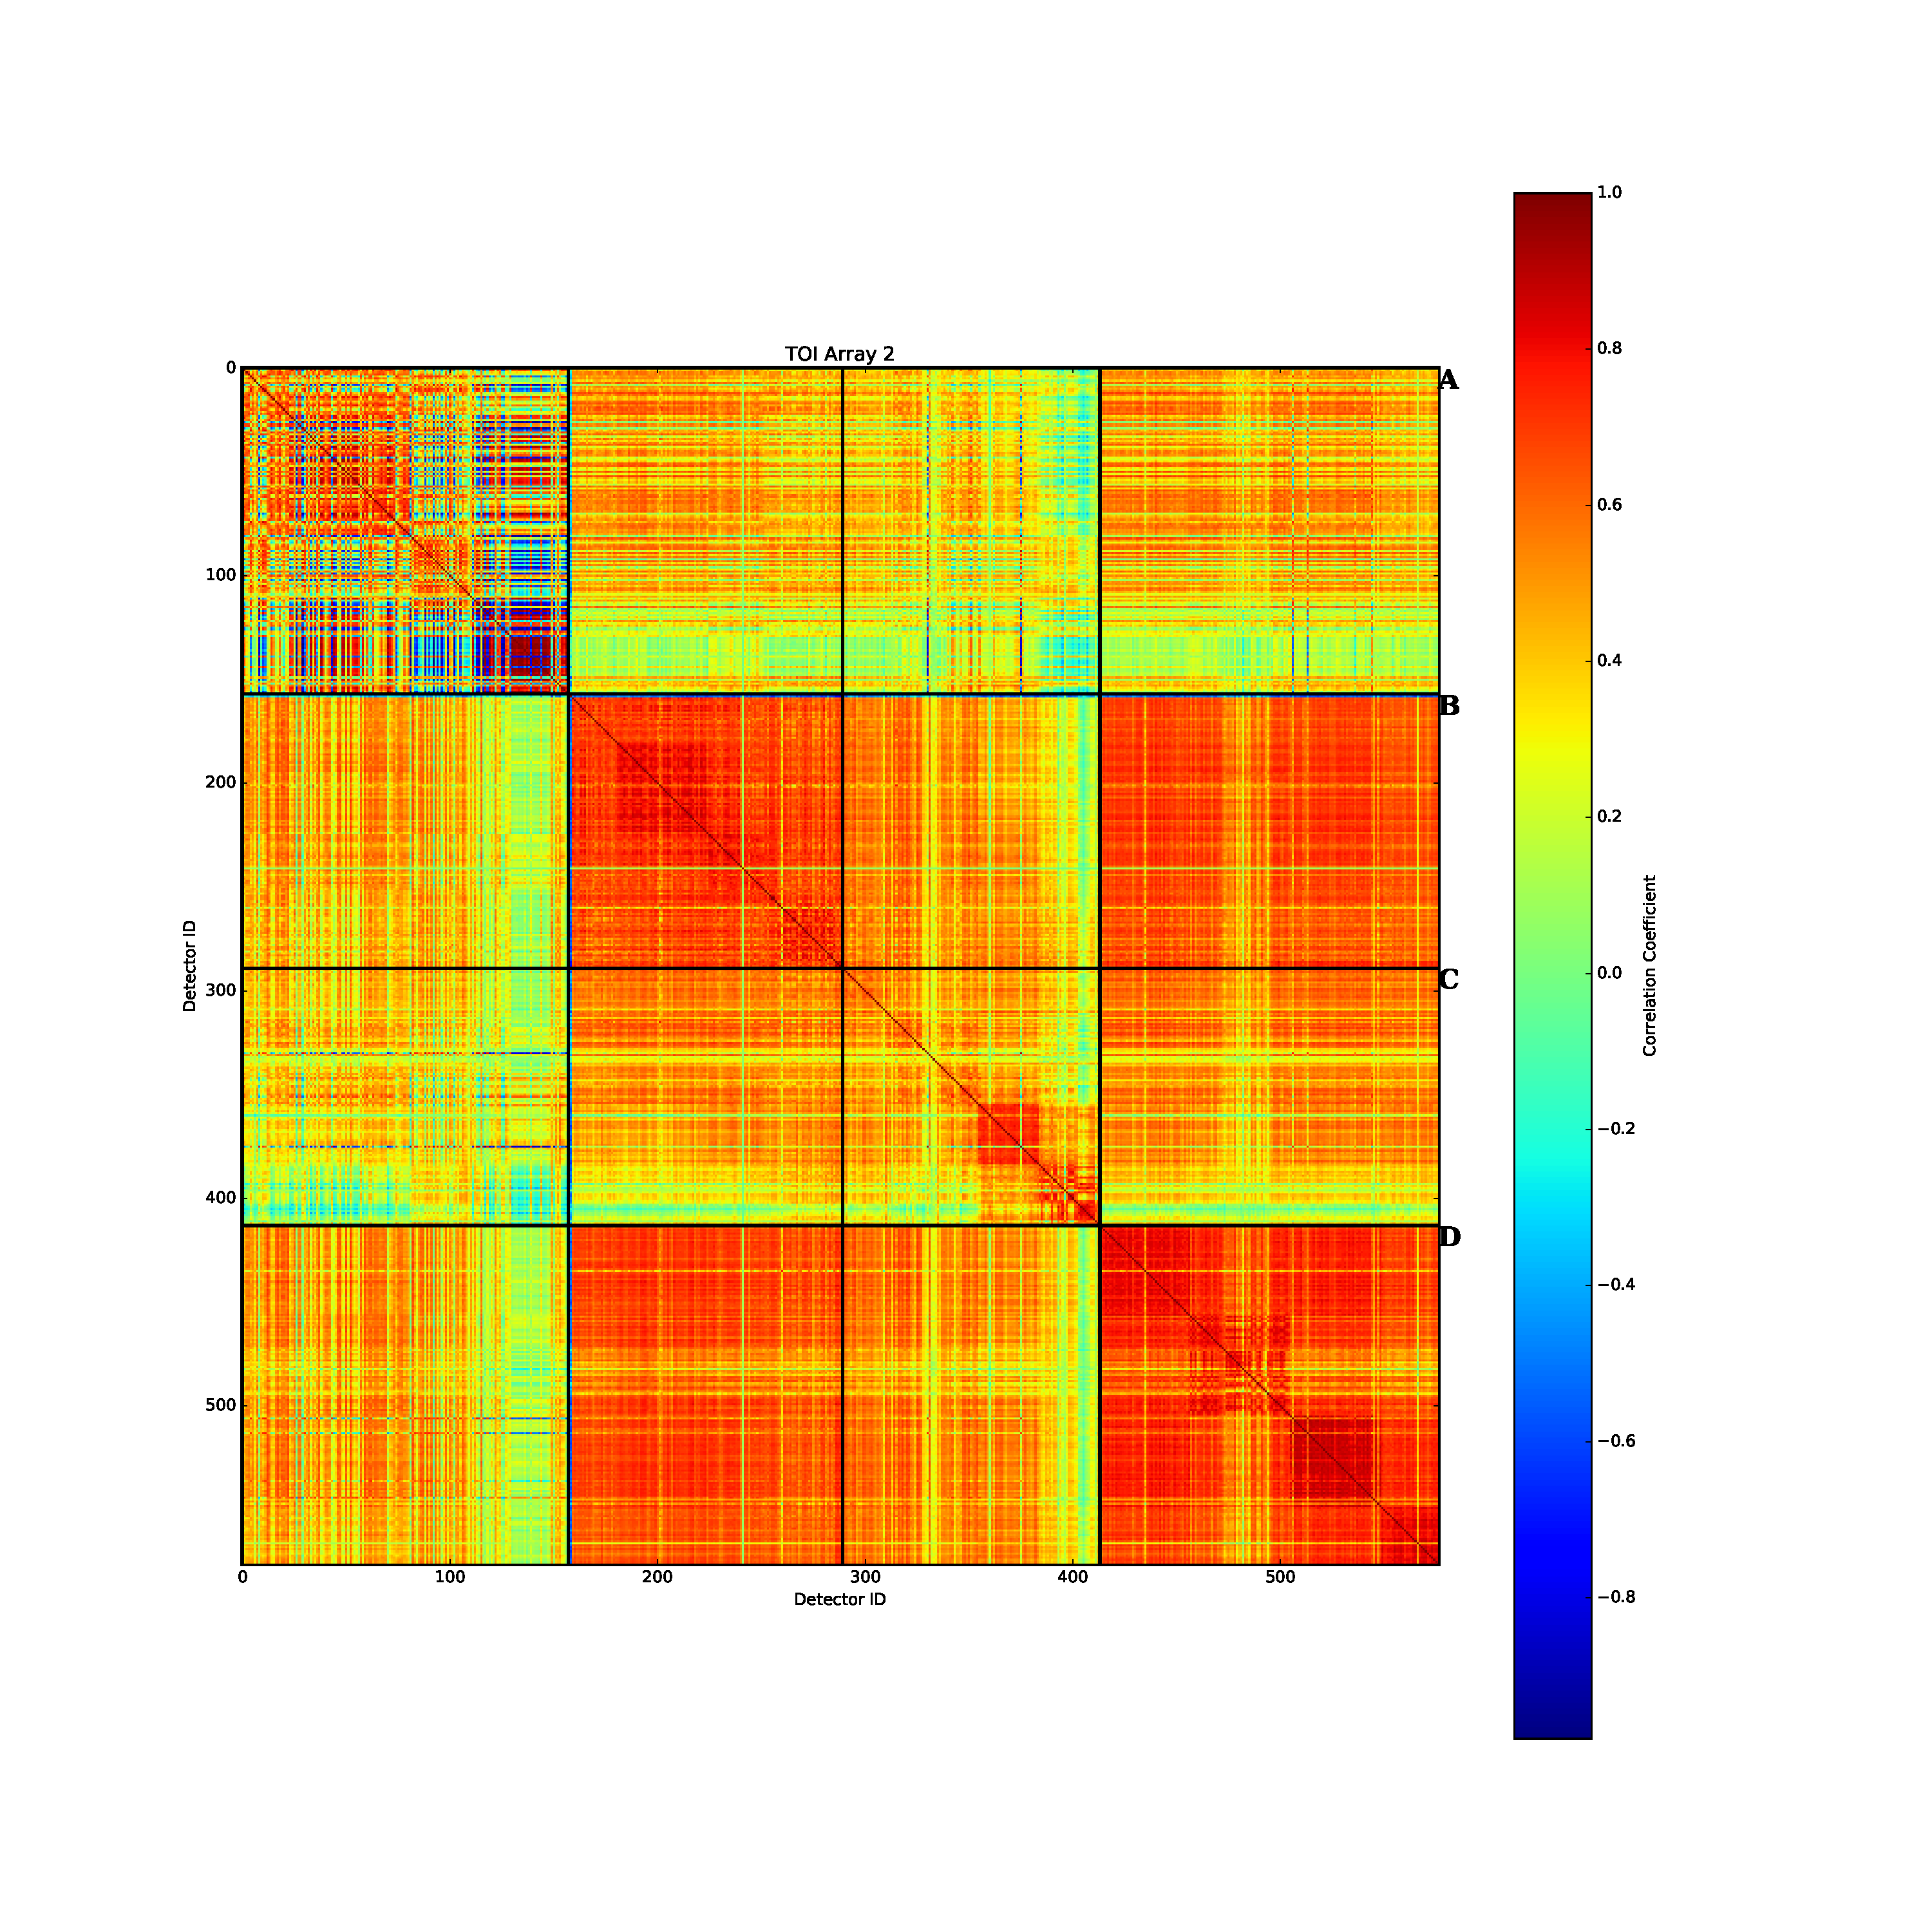
\includegraphics[width=0.3\textwidth]{Figures/DarkTests/corrmat_TOI_array_2_20161211s299.pdf}
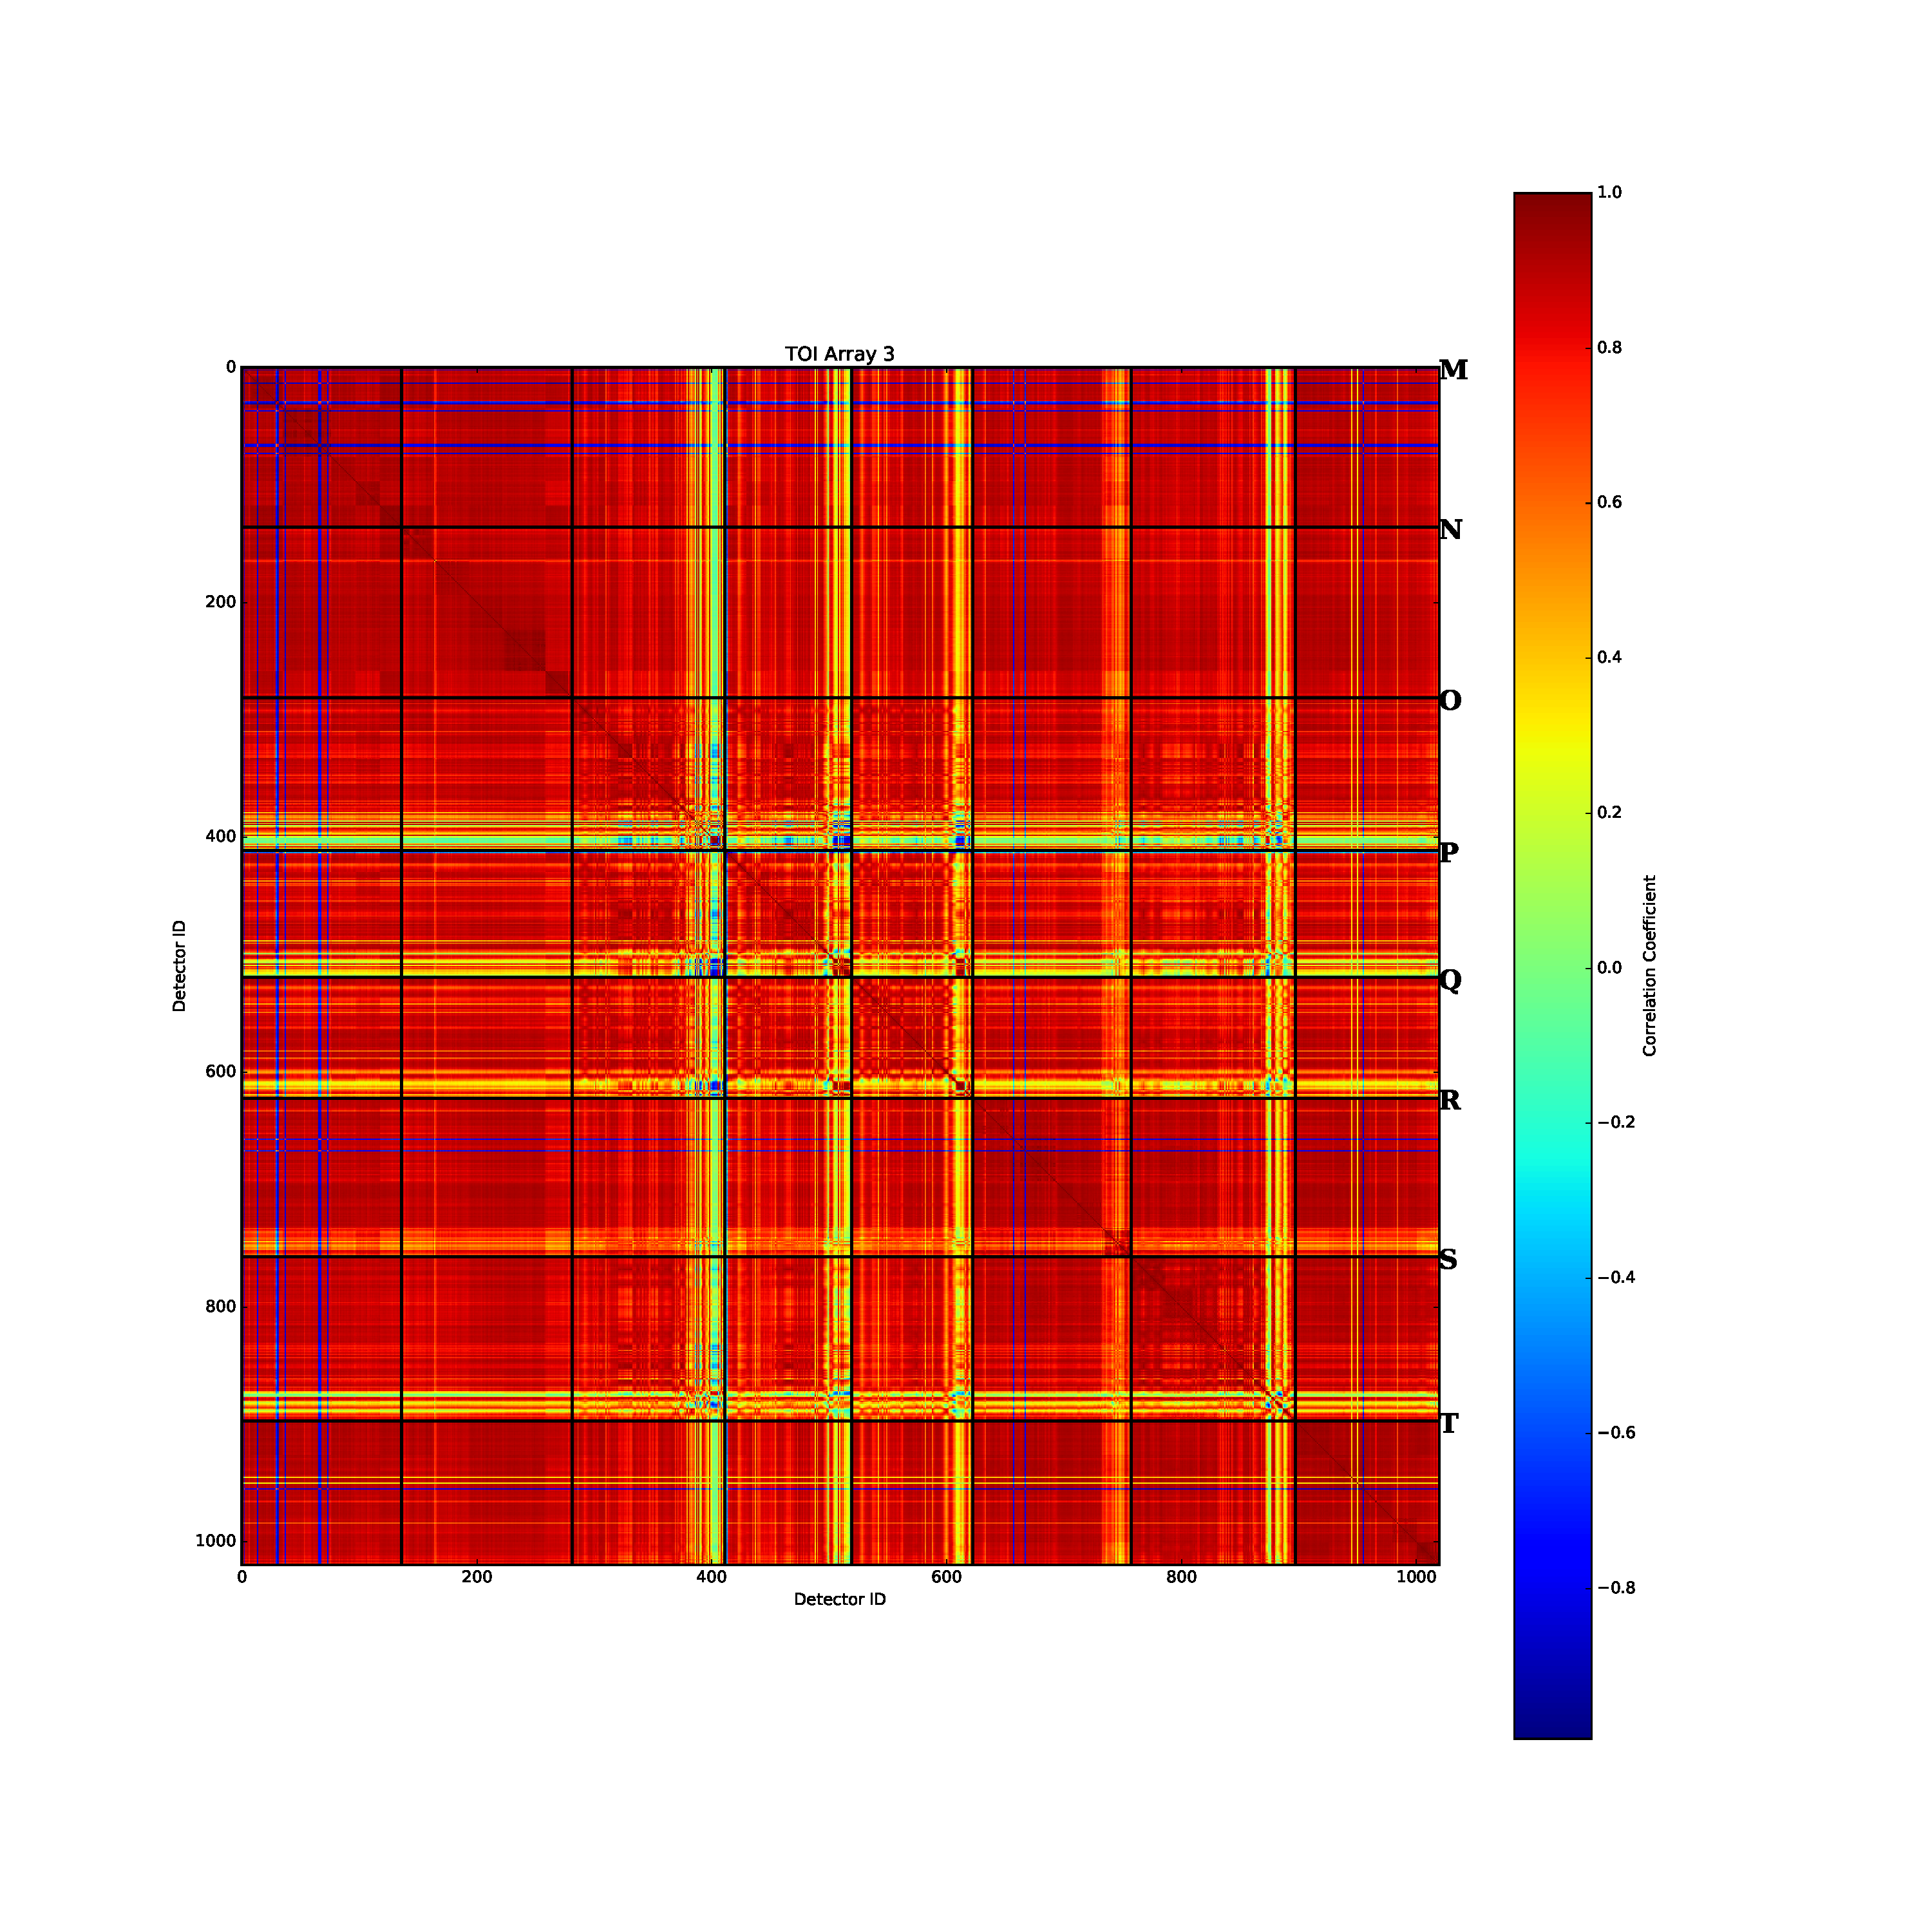
\includegraphics[width=0.3\textwidth]{Figures/DarkTests/corrmat_TOI_array_3_20161211s299.pdf}
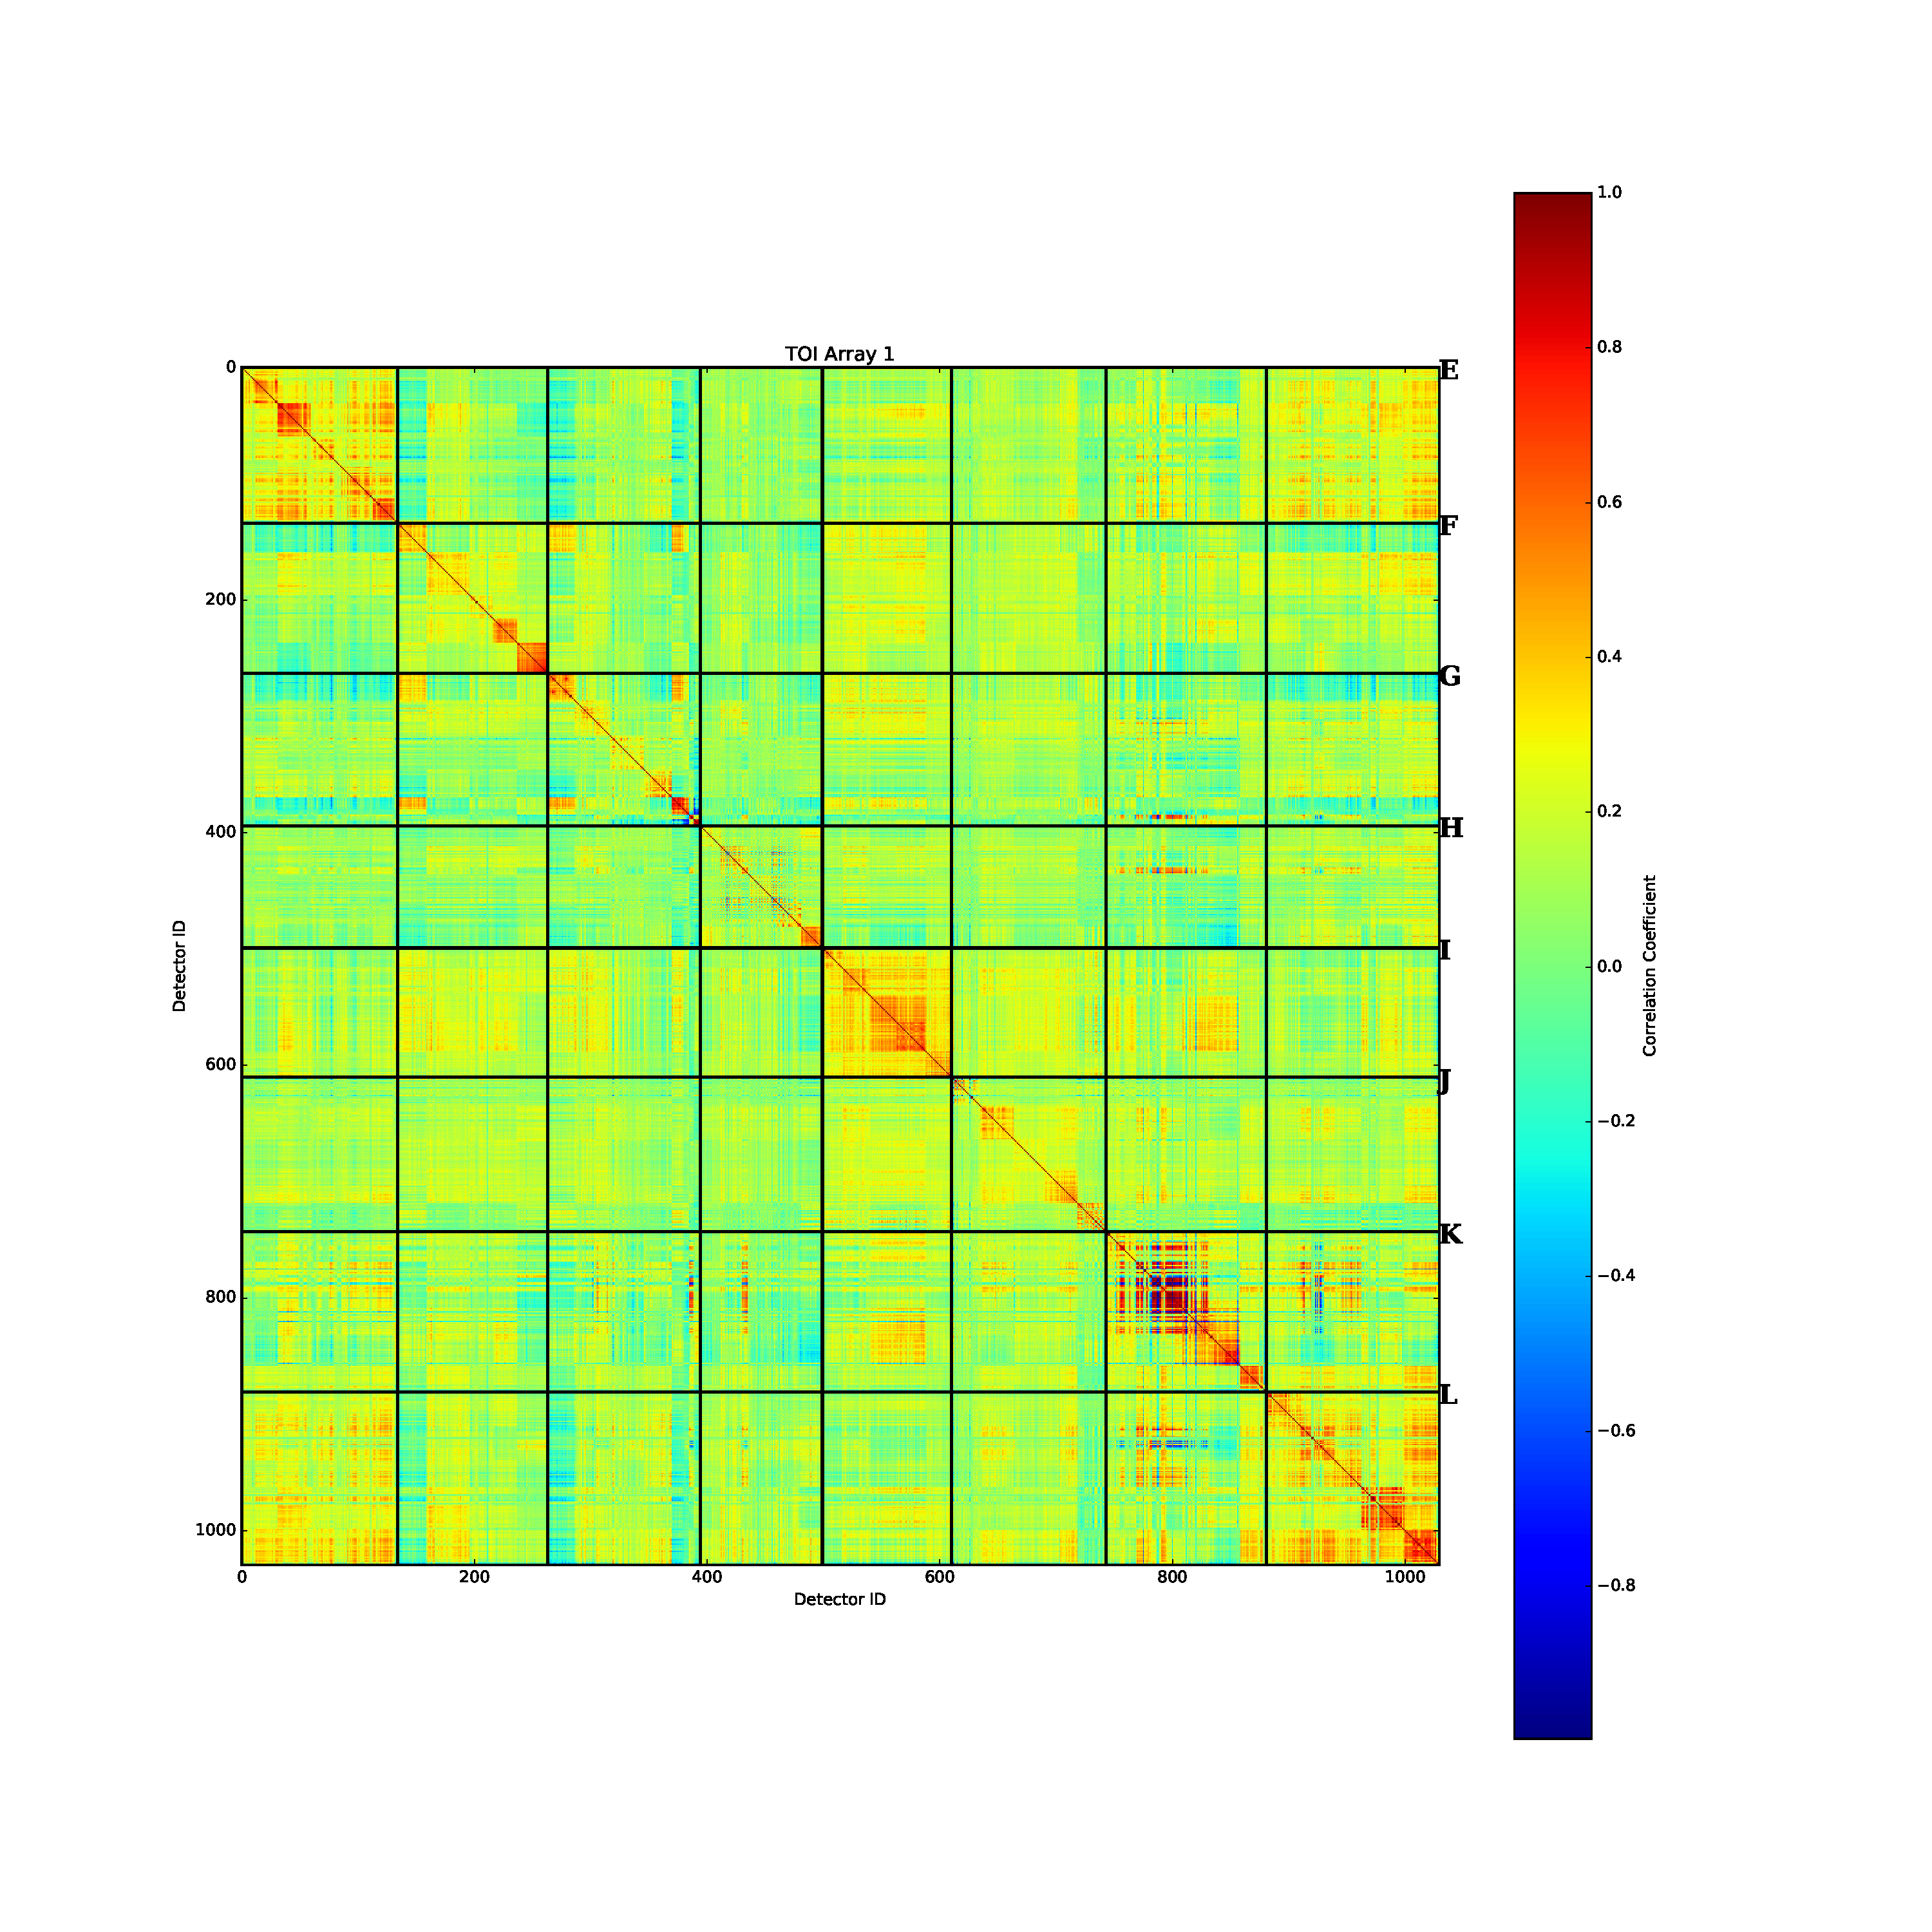
\includegraphics[width=0.3\textwidth]{Figures/DarkTests/corrmat_TOI_CM_array_1_20161211s299.pdf}
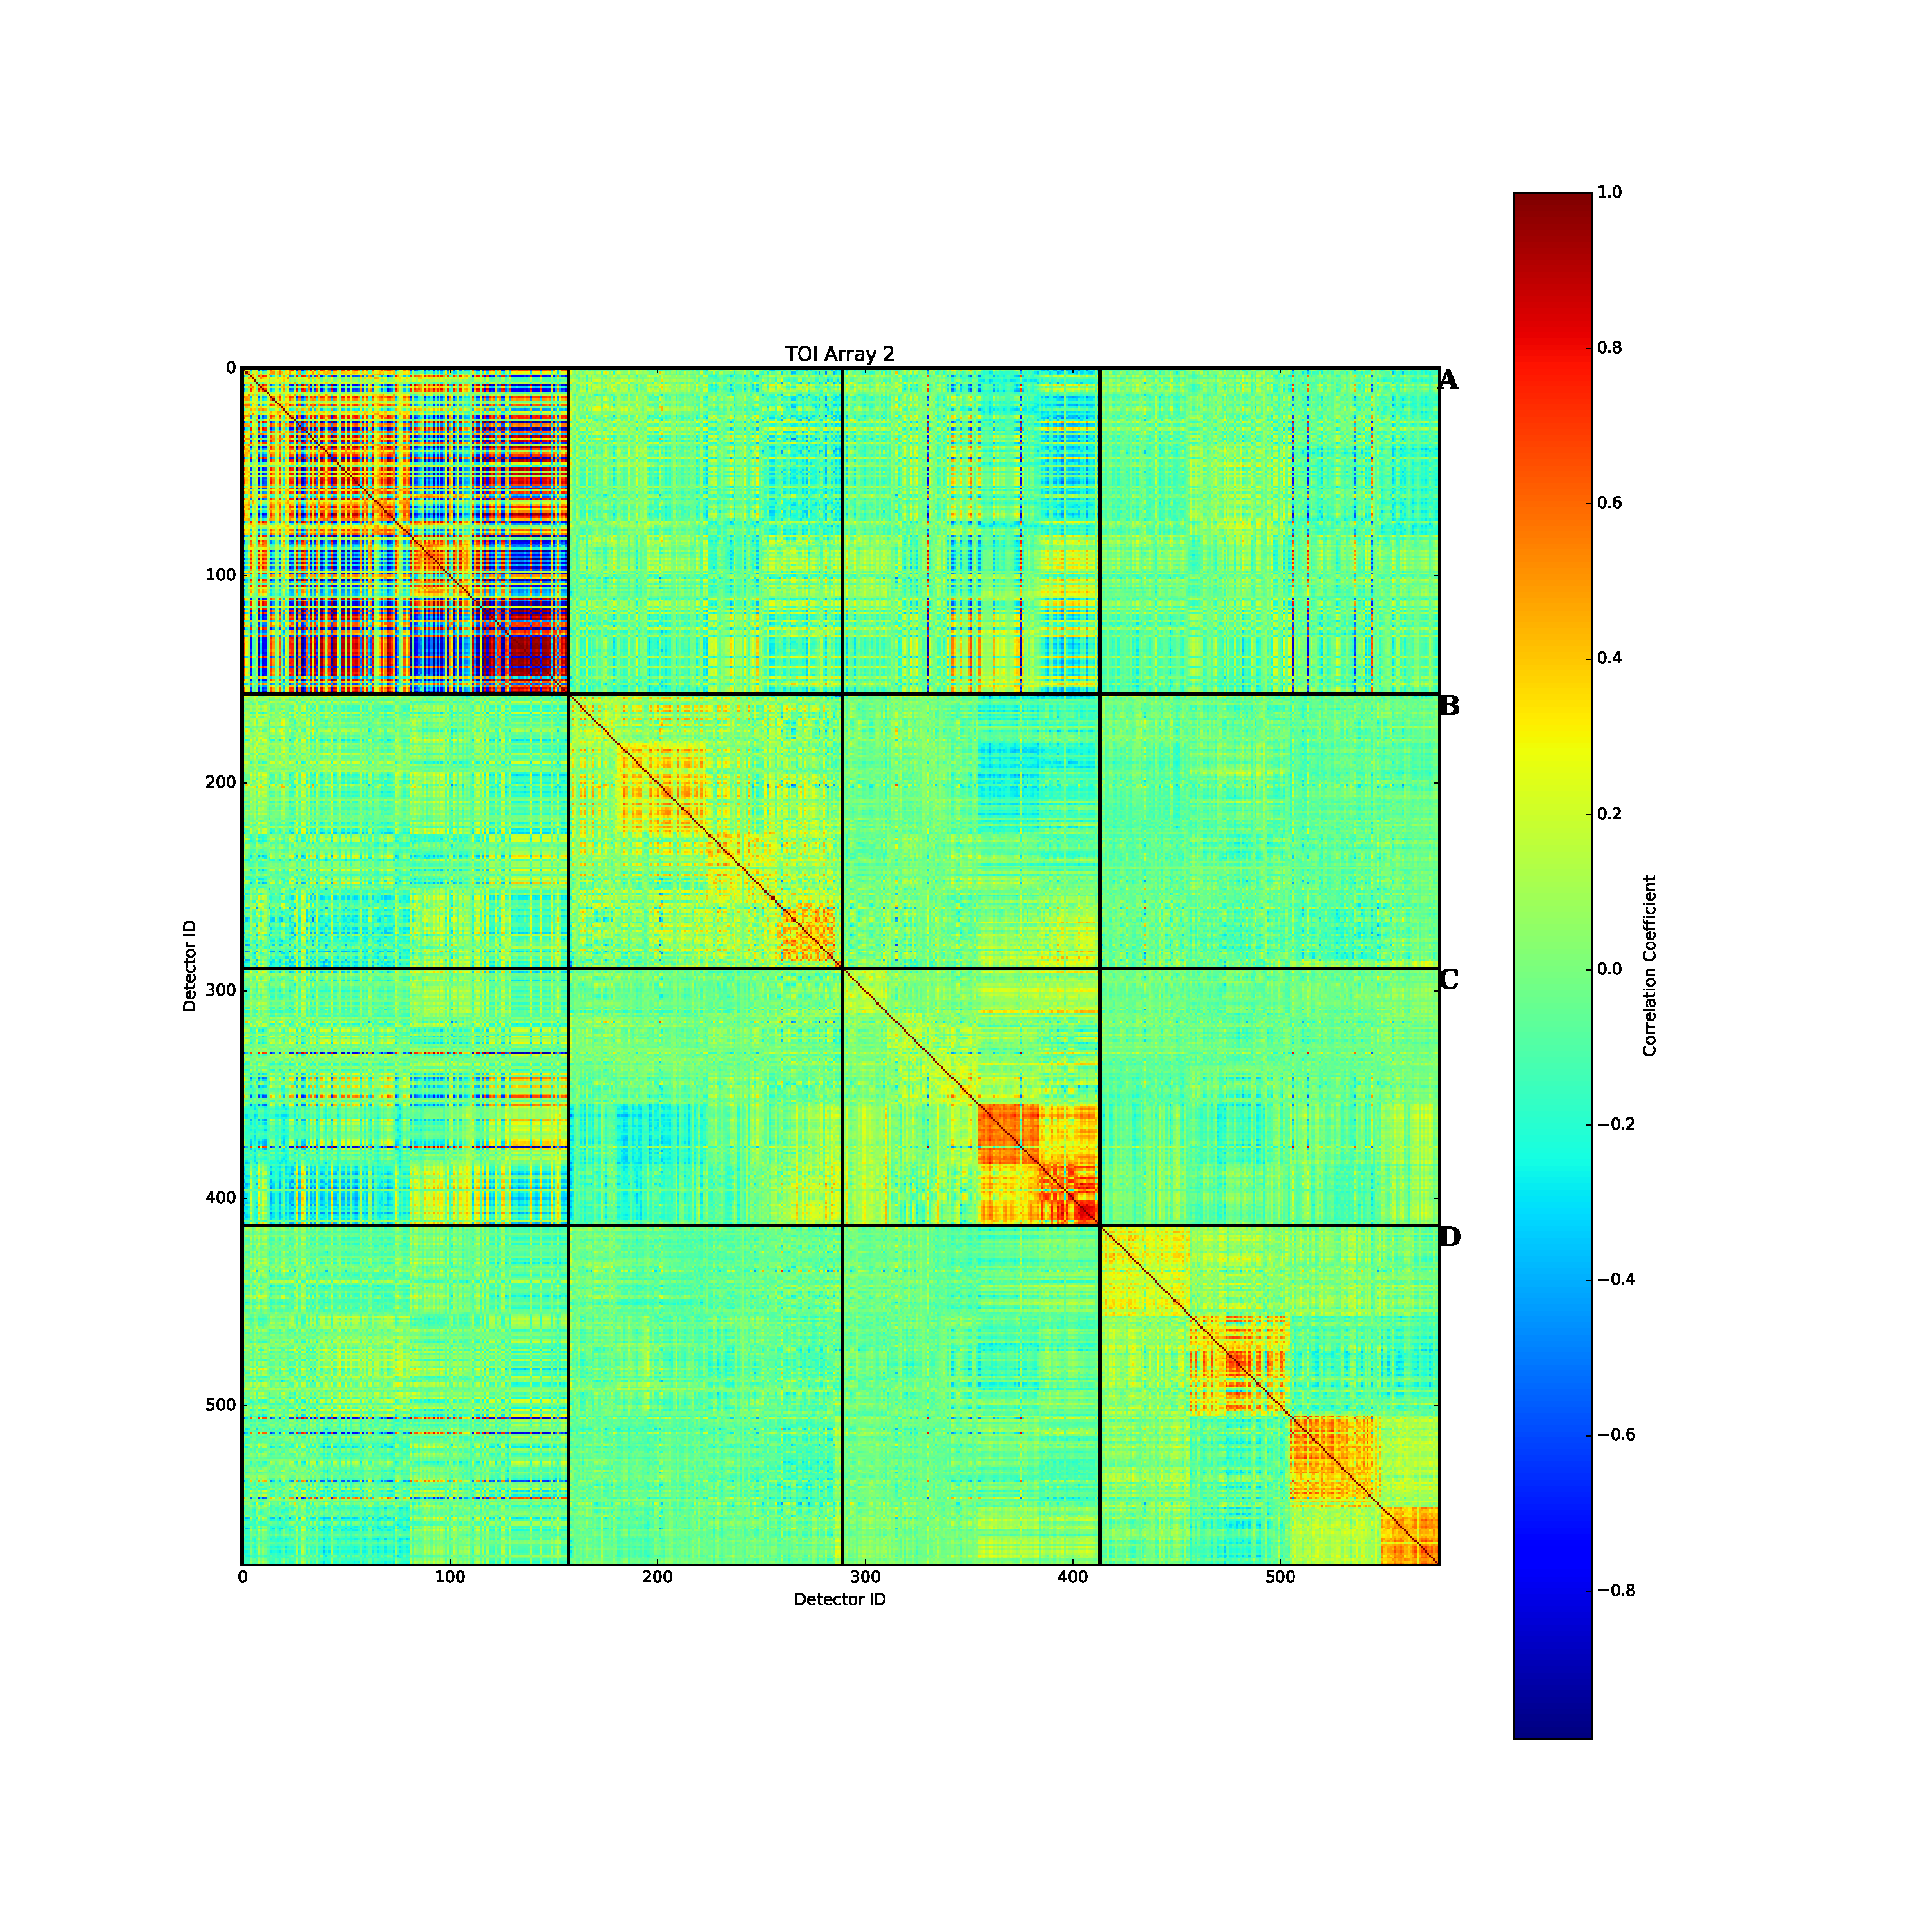
\includegraphics[width=0.3\textwidth]{Figures/DarkTests/corrmat_TOI_CM_array_2_20161211s299.pdf}
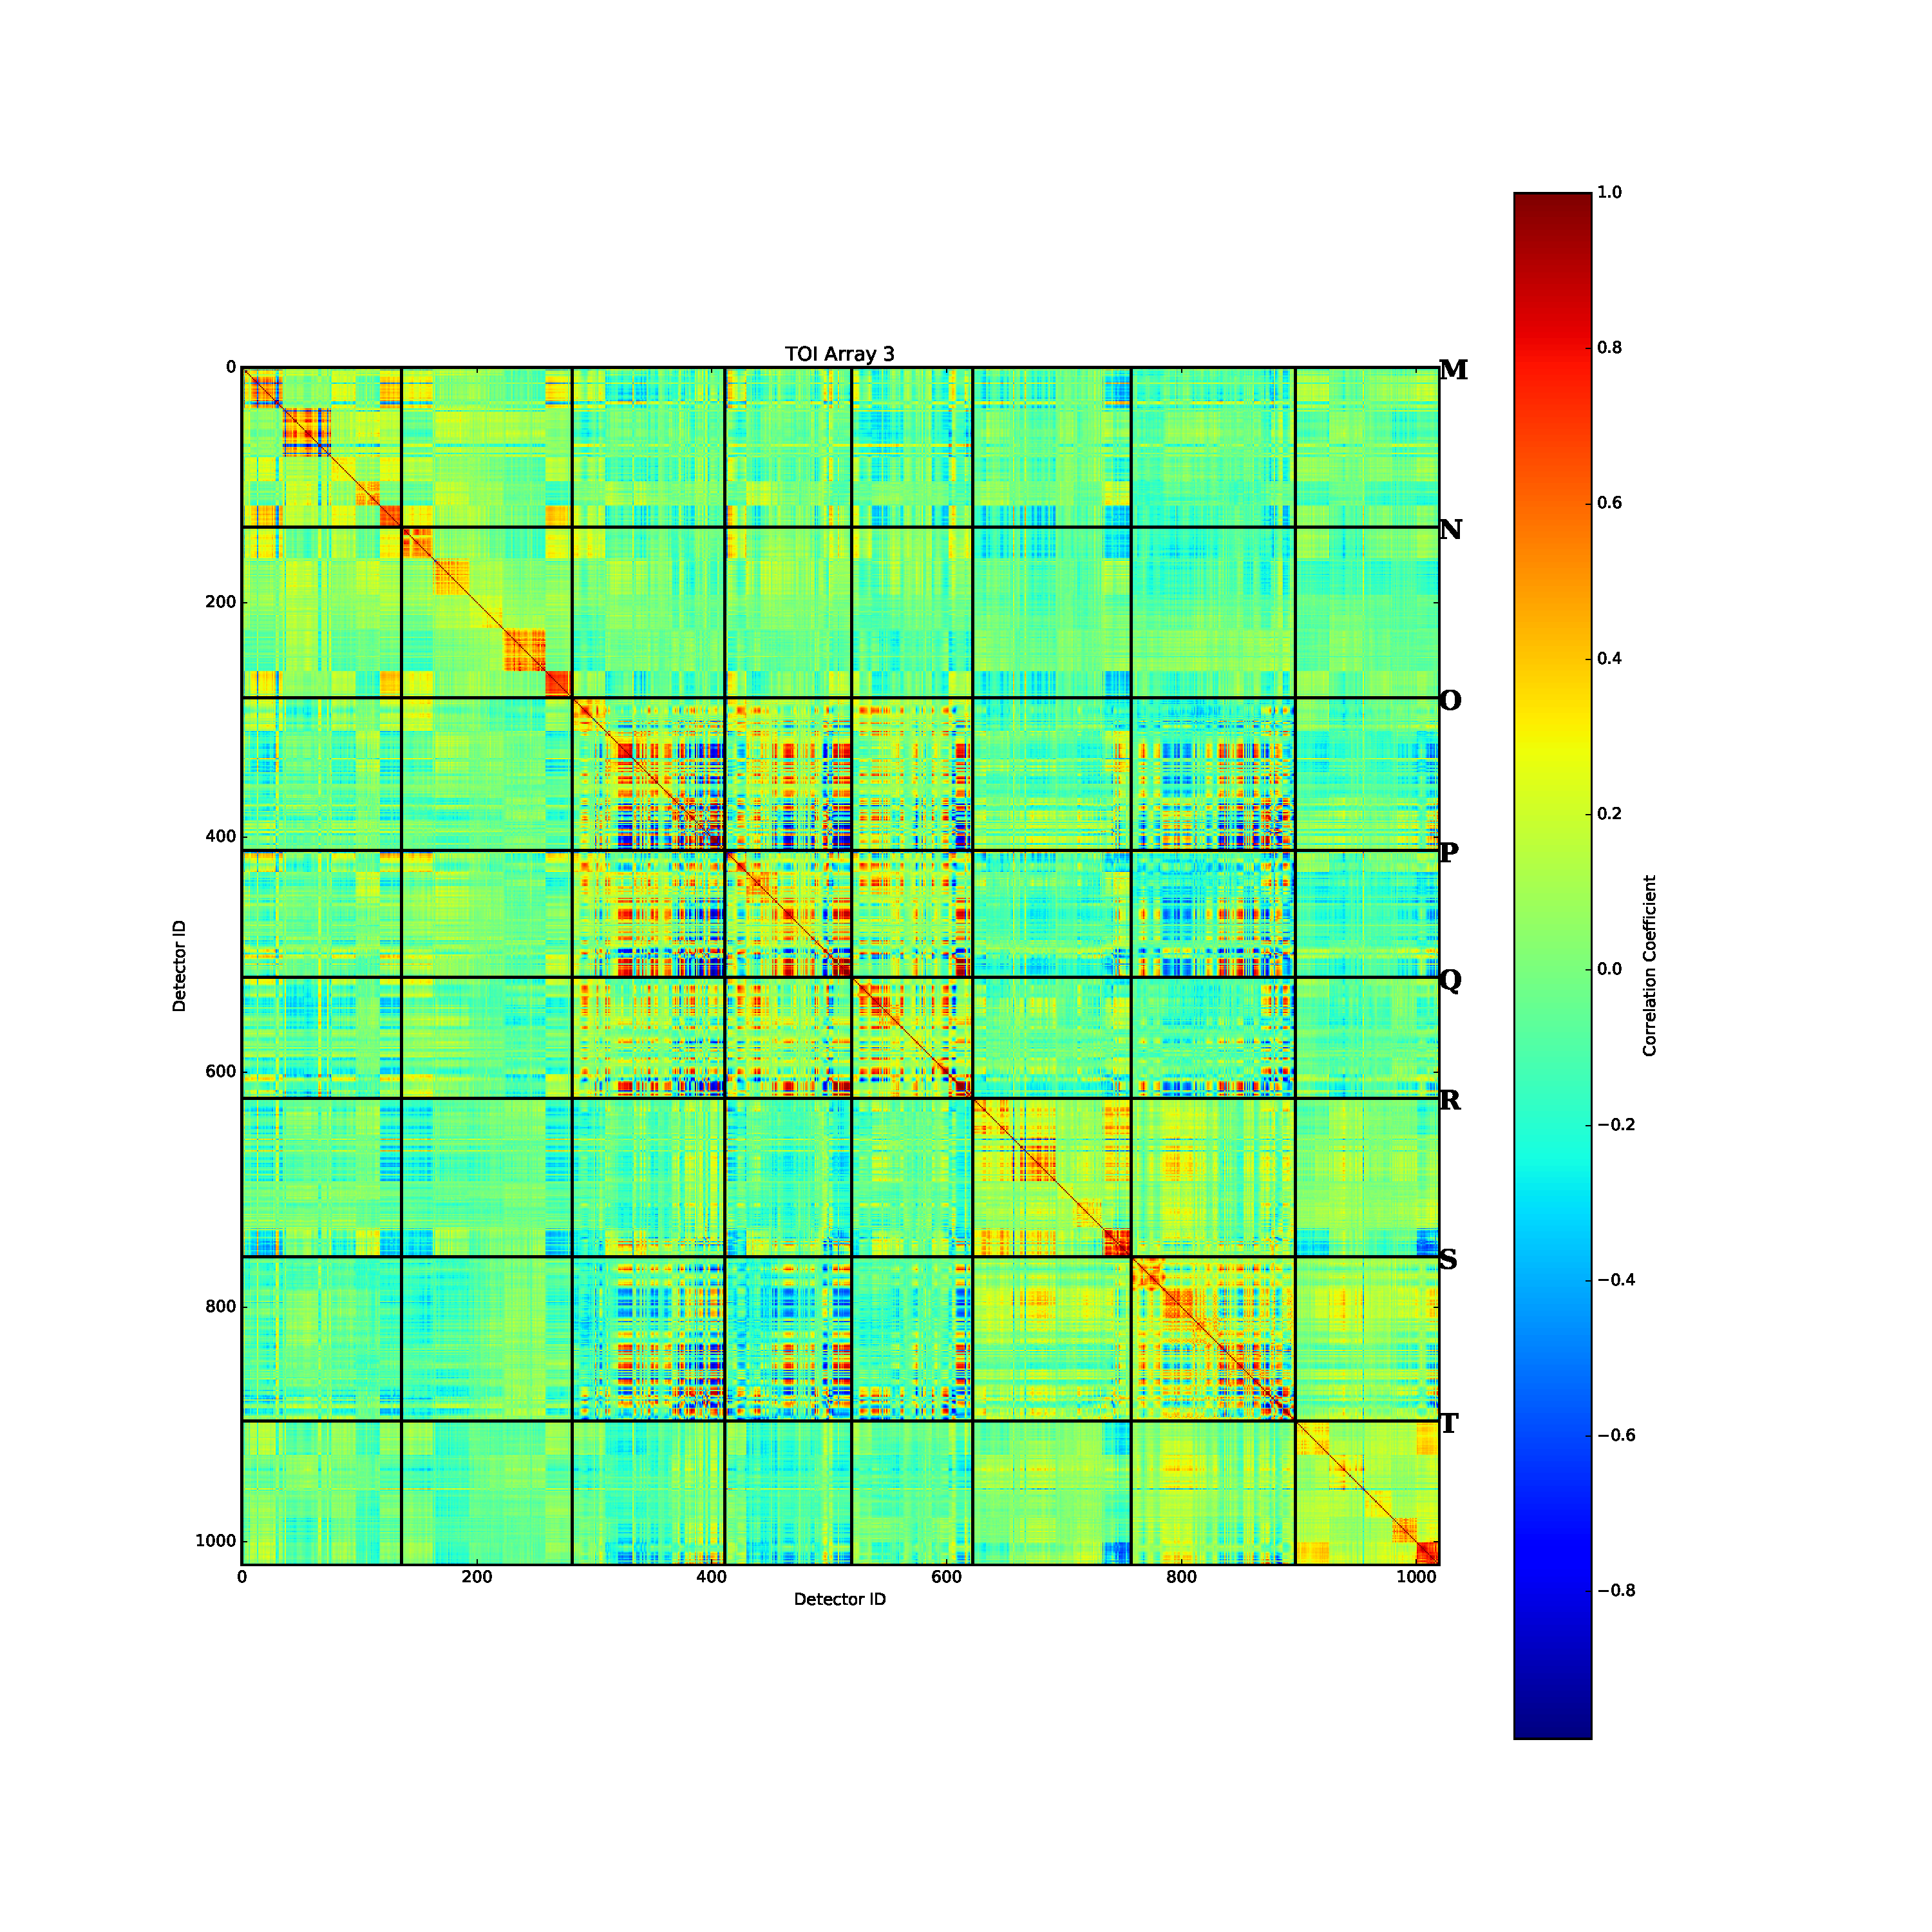
\includegraphics[width=0.3\textwidth]{Figures/DarkTests/corrmat_TOI_CM_array_3_20161211s299.pdf}
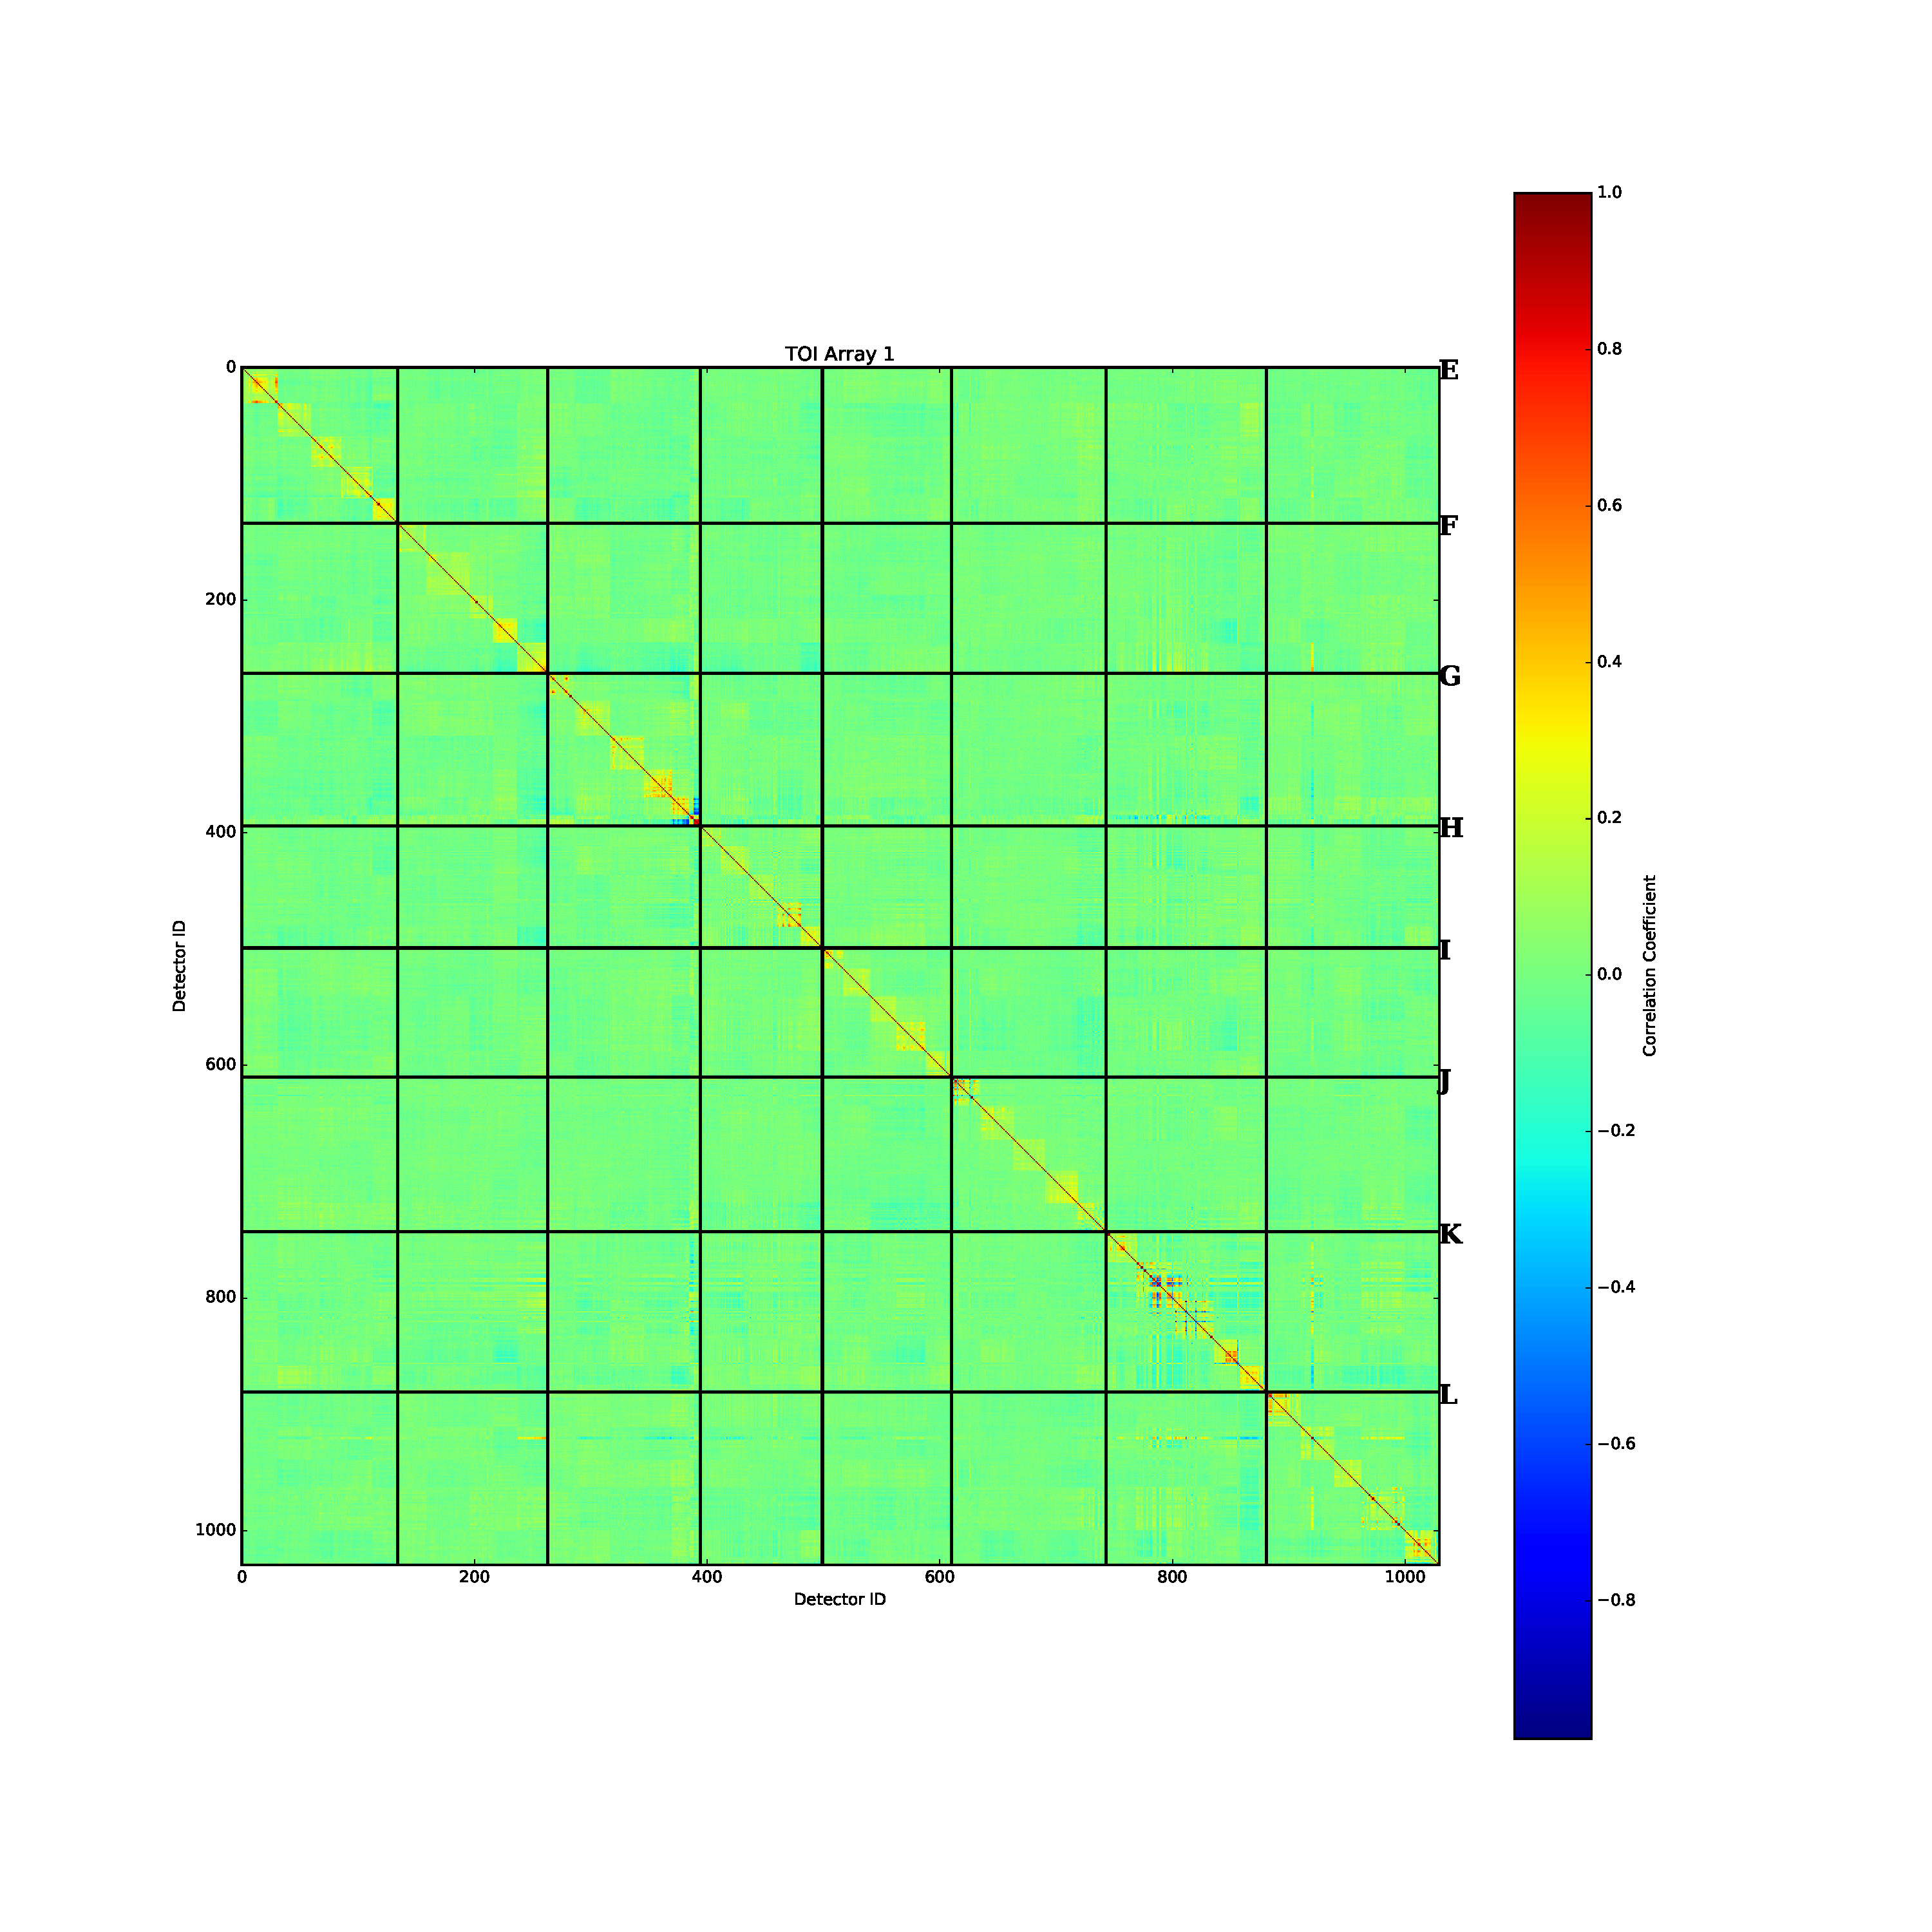
\includegraphics[width=0.3\textwidth]{Figures/DarkTests/corrmat_TOI_PCA_array_1_20161211s299.pdf}
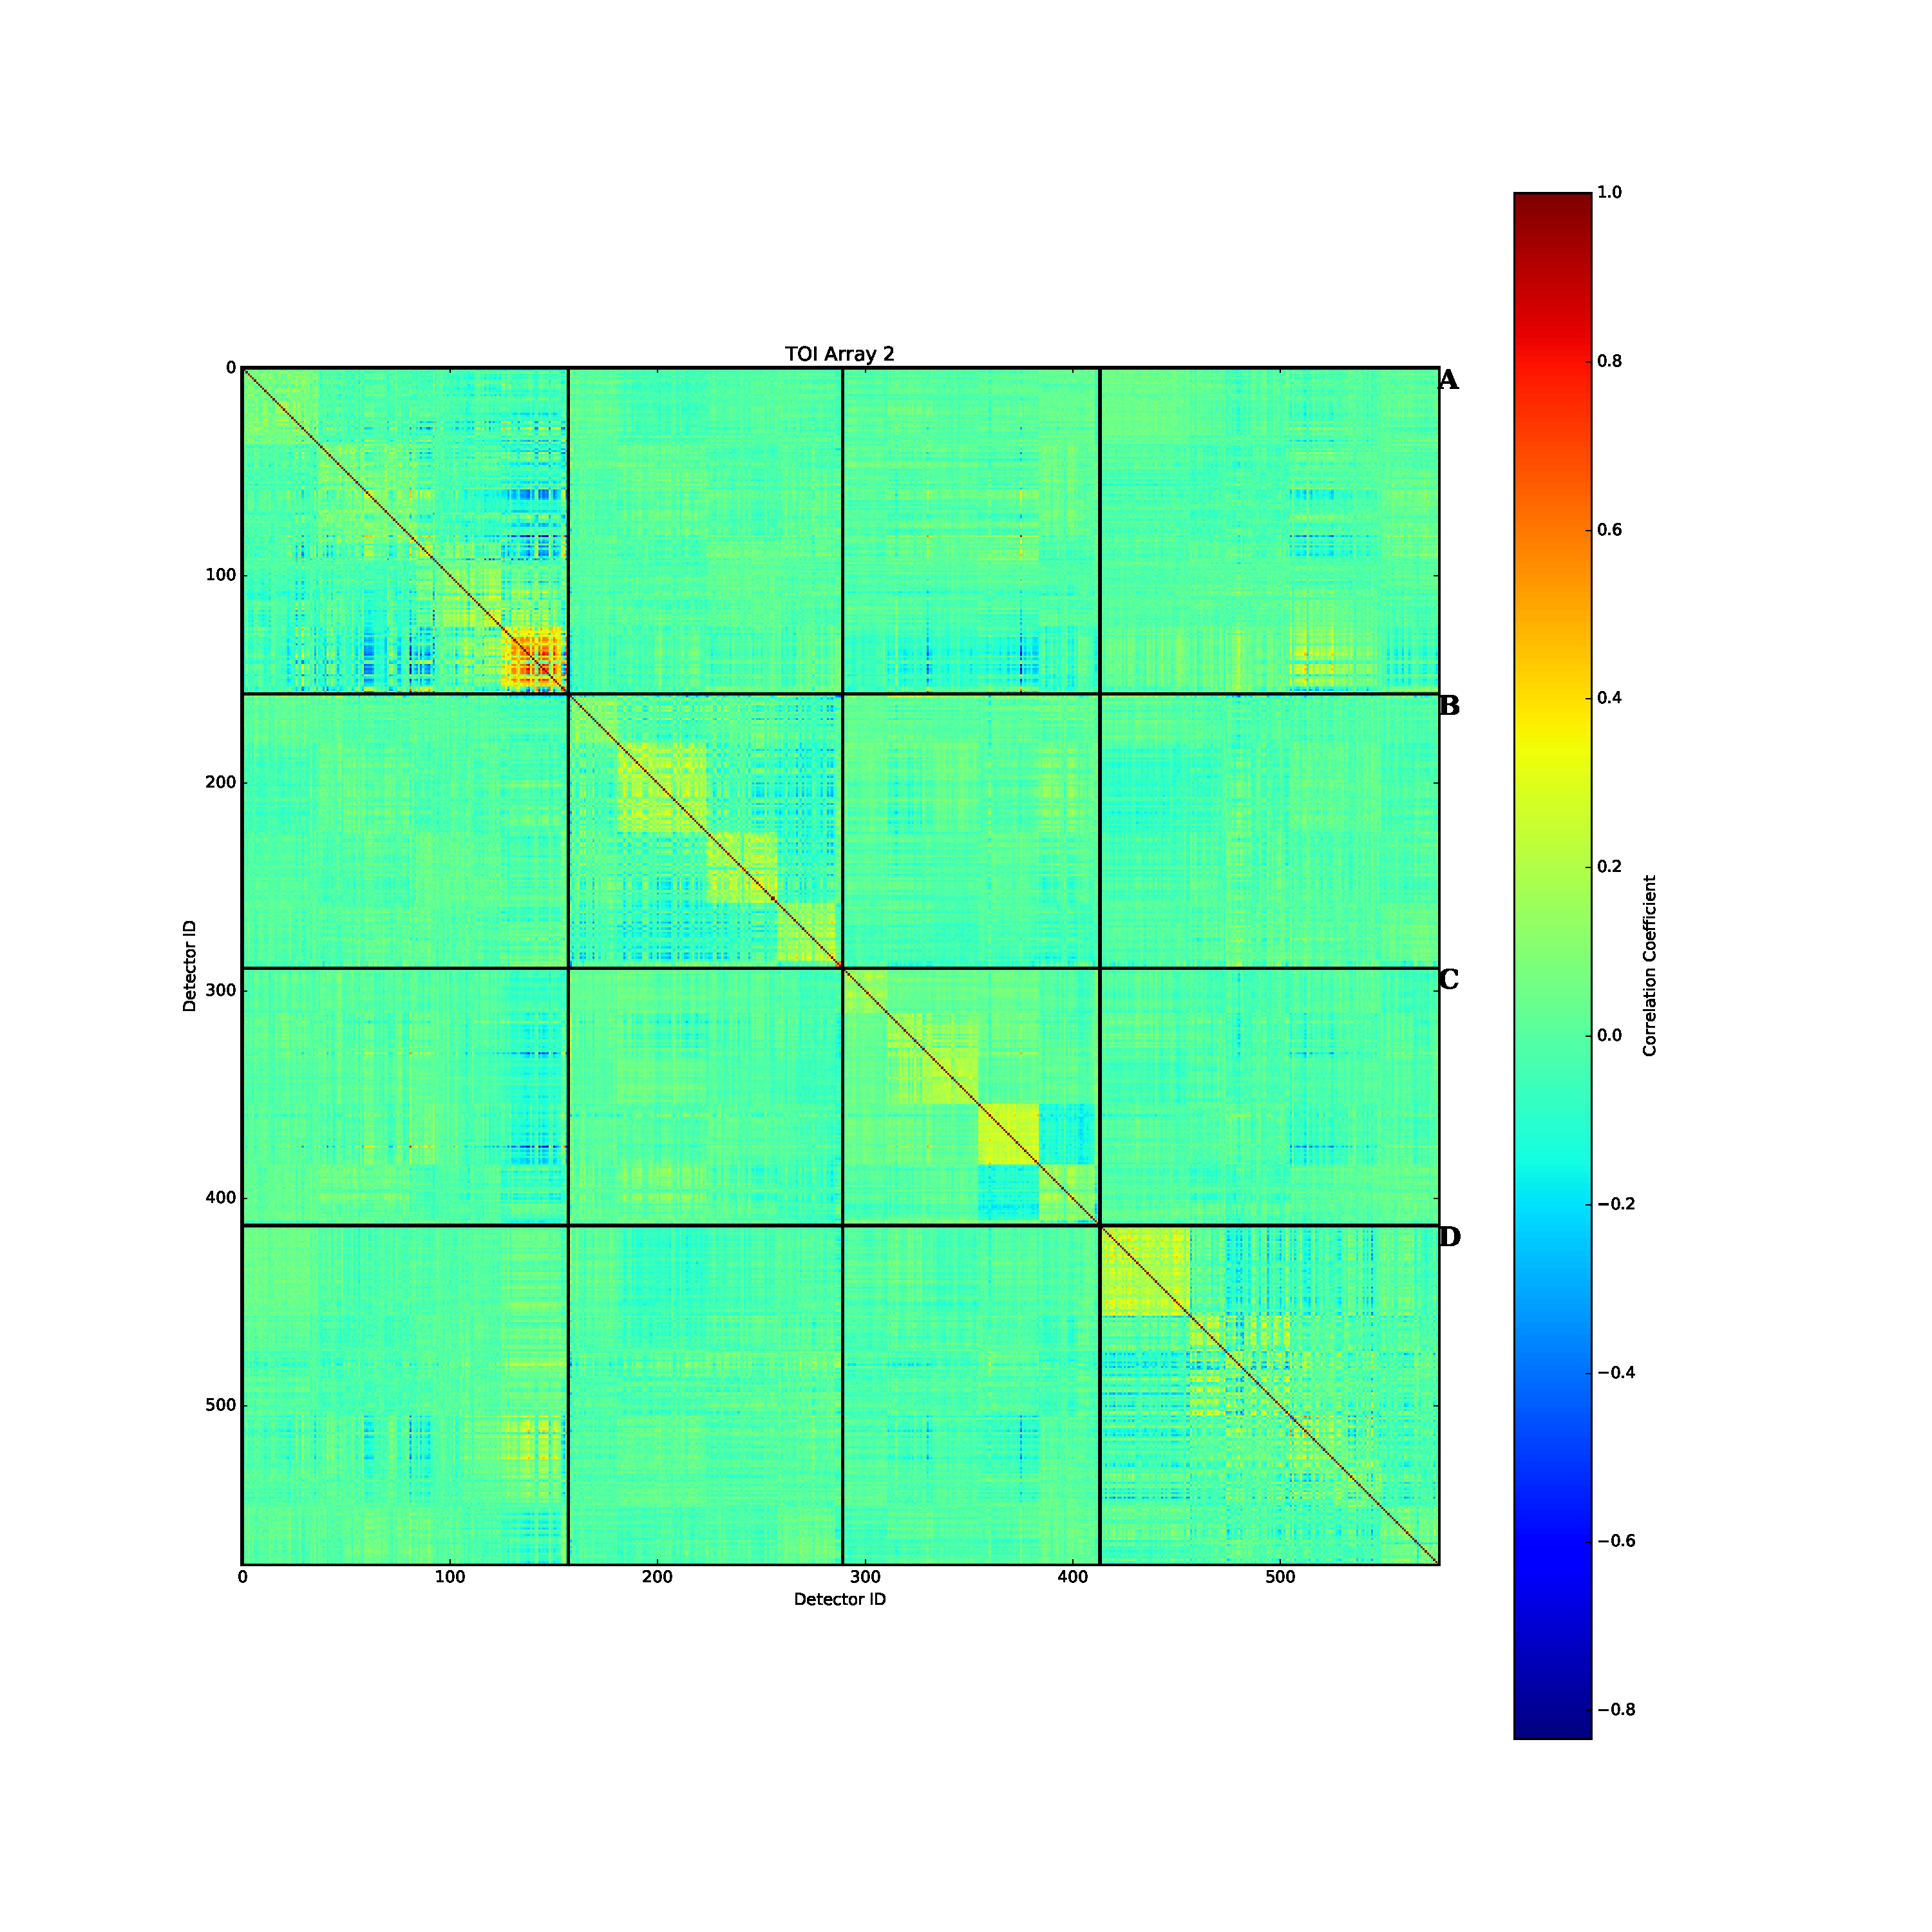
\includegraphics[width=0.3\textwidth]{Figures/DarkTests/corrmat_TOI_PCA_array_2_20161211s299.pdf}
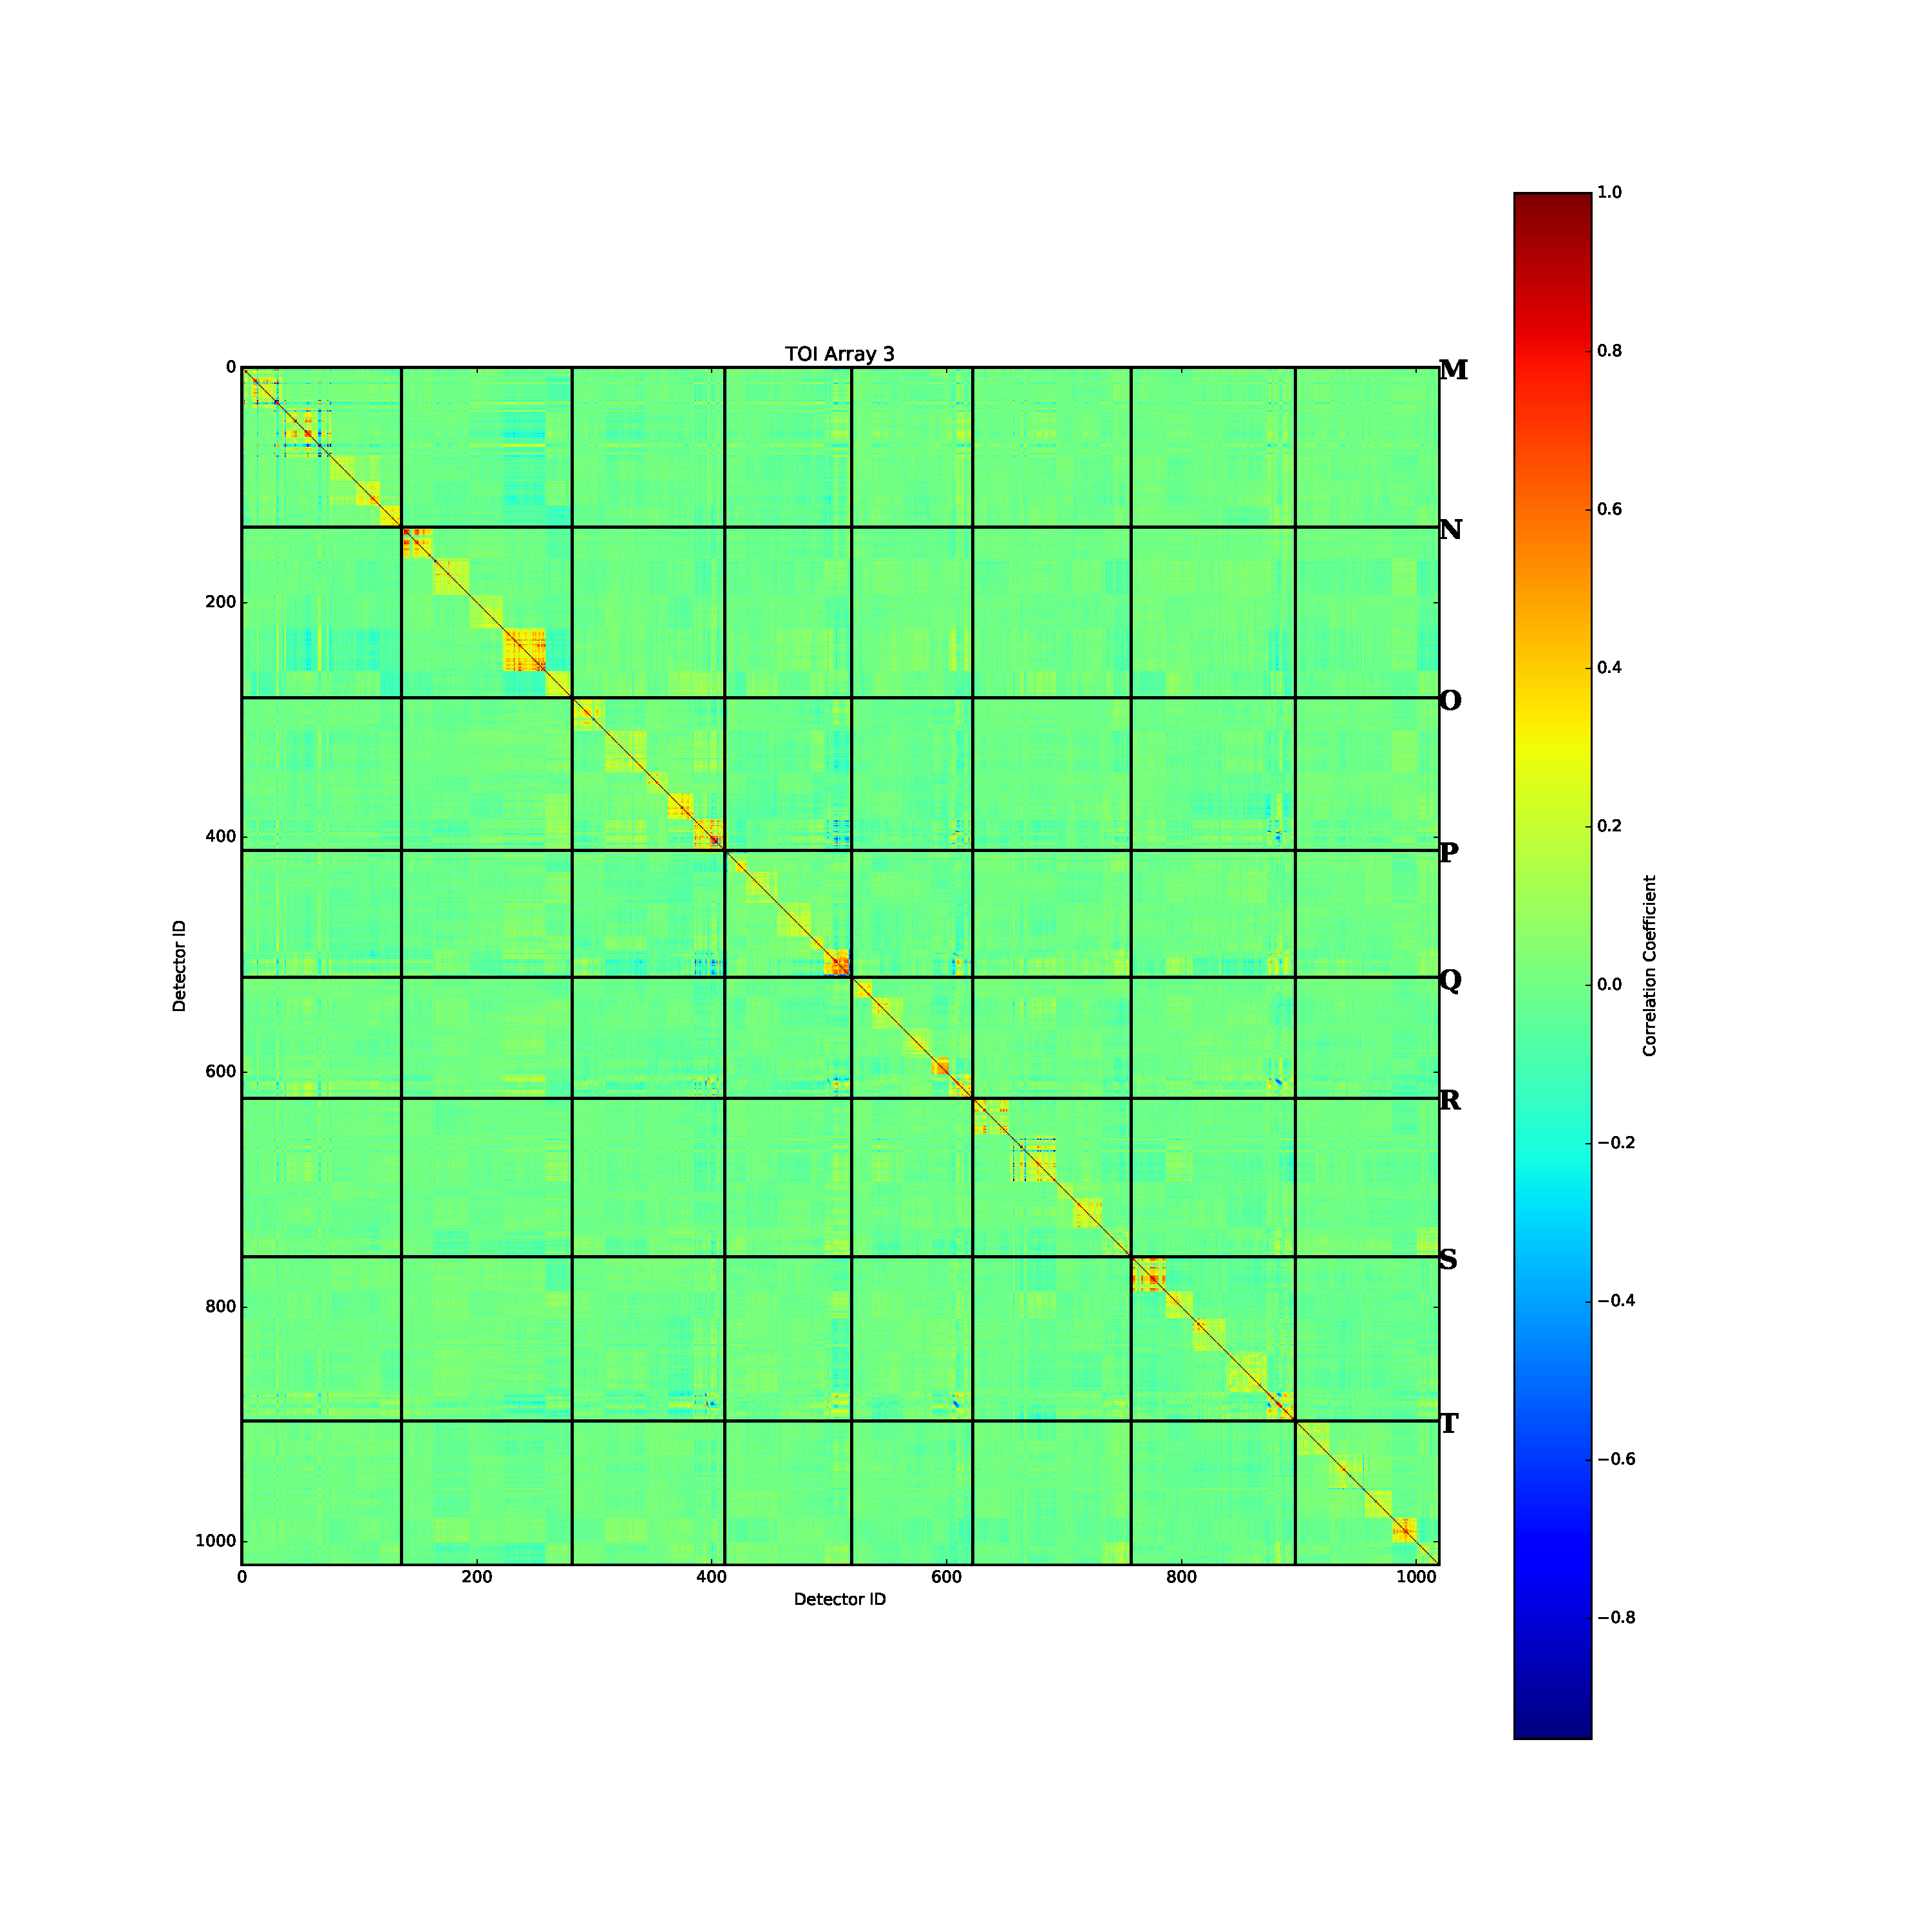
\includegraphics[width=0.3\textwidth]{Figures/DarkTests/corrmat_TOI_PCA_array_3_20161211s299.pdf}
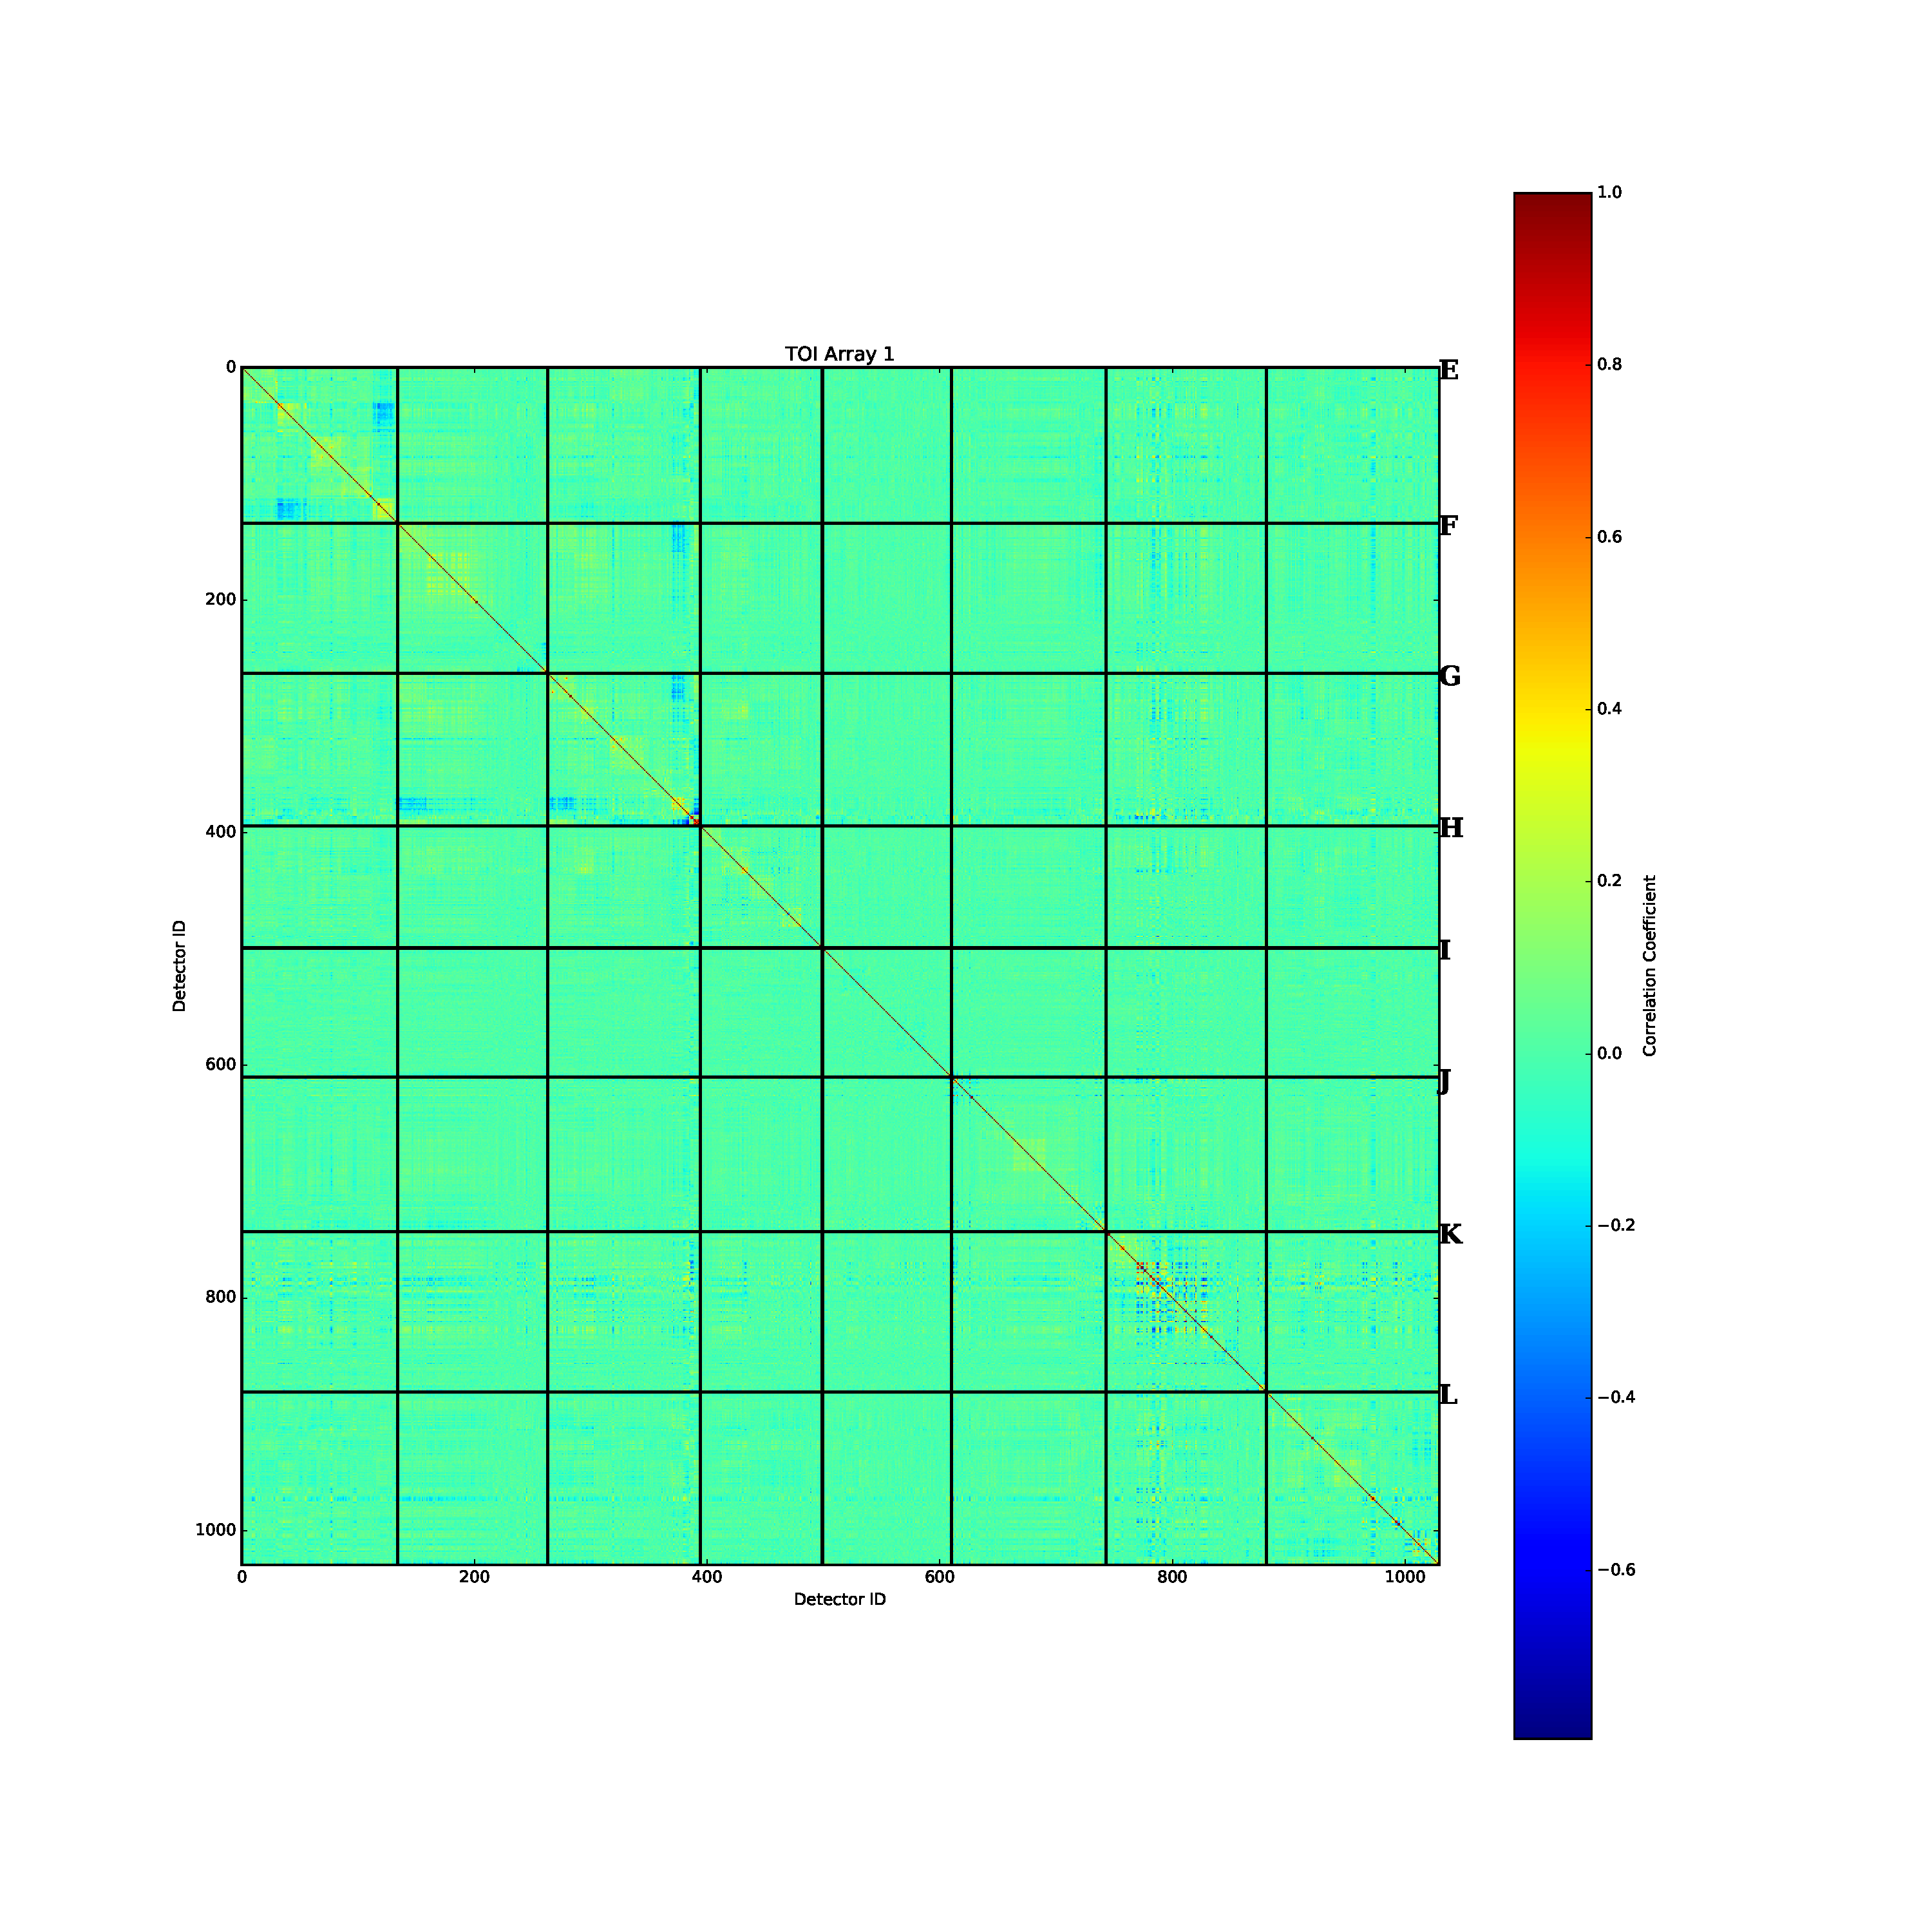
\includegraphics[width=0.3\textwidth]{Figures/DarkTests/corrmat_TOI_BC_array_1_20161211s299.pdf}
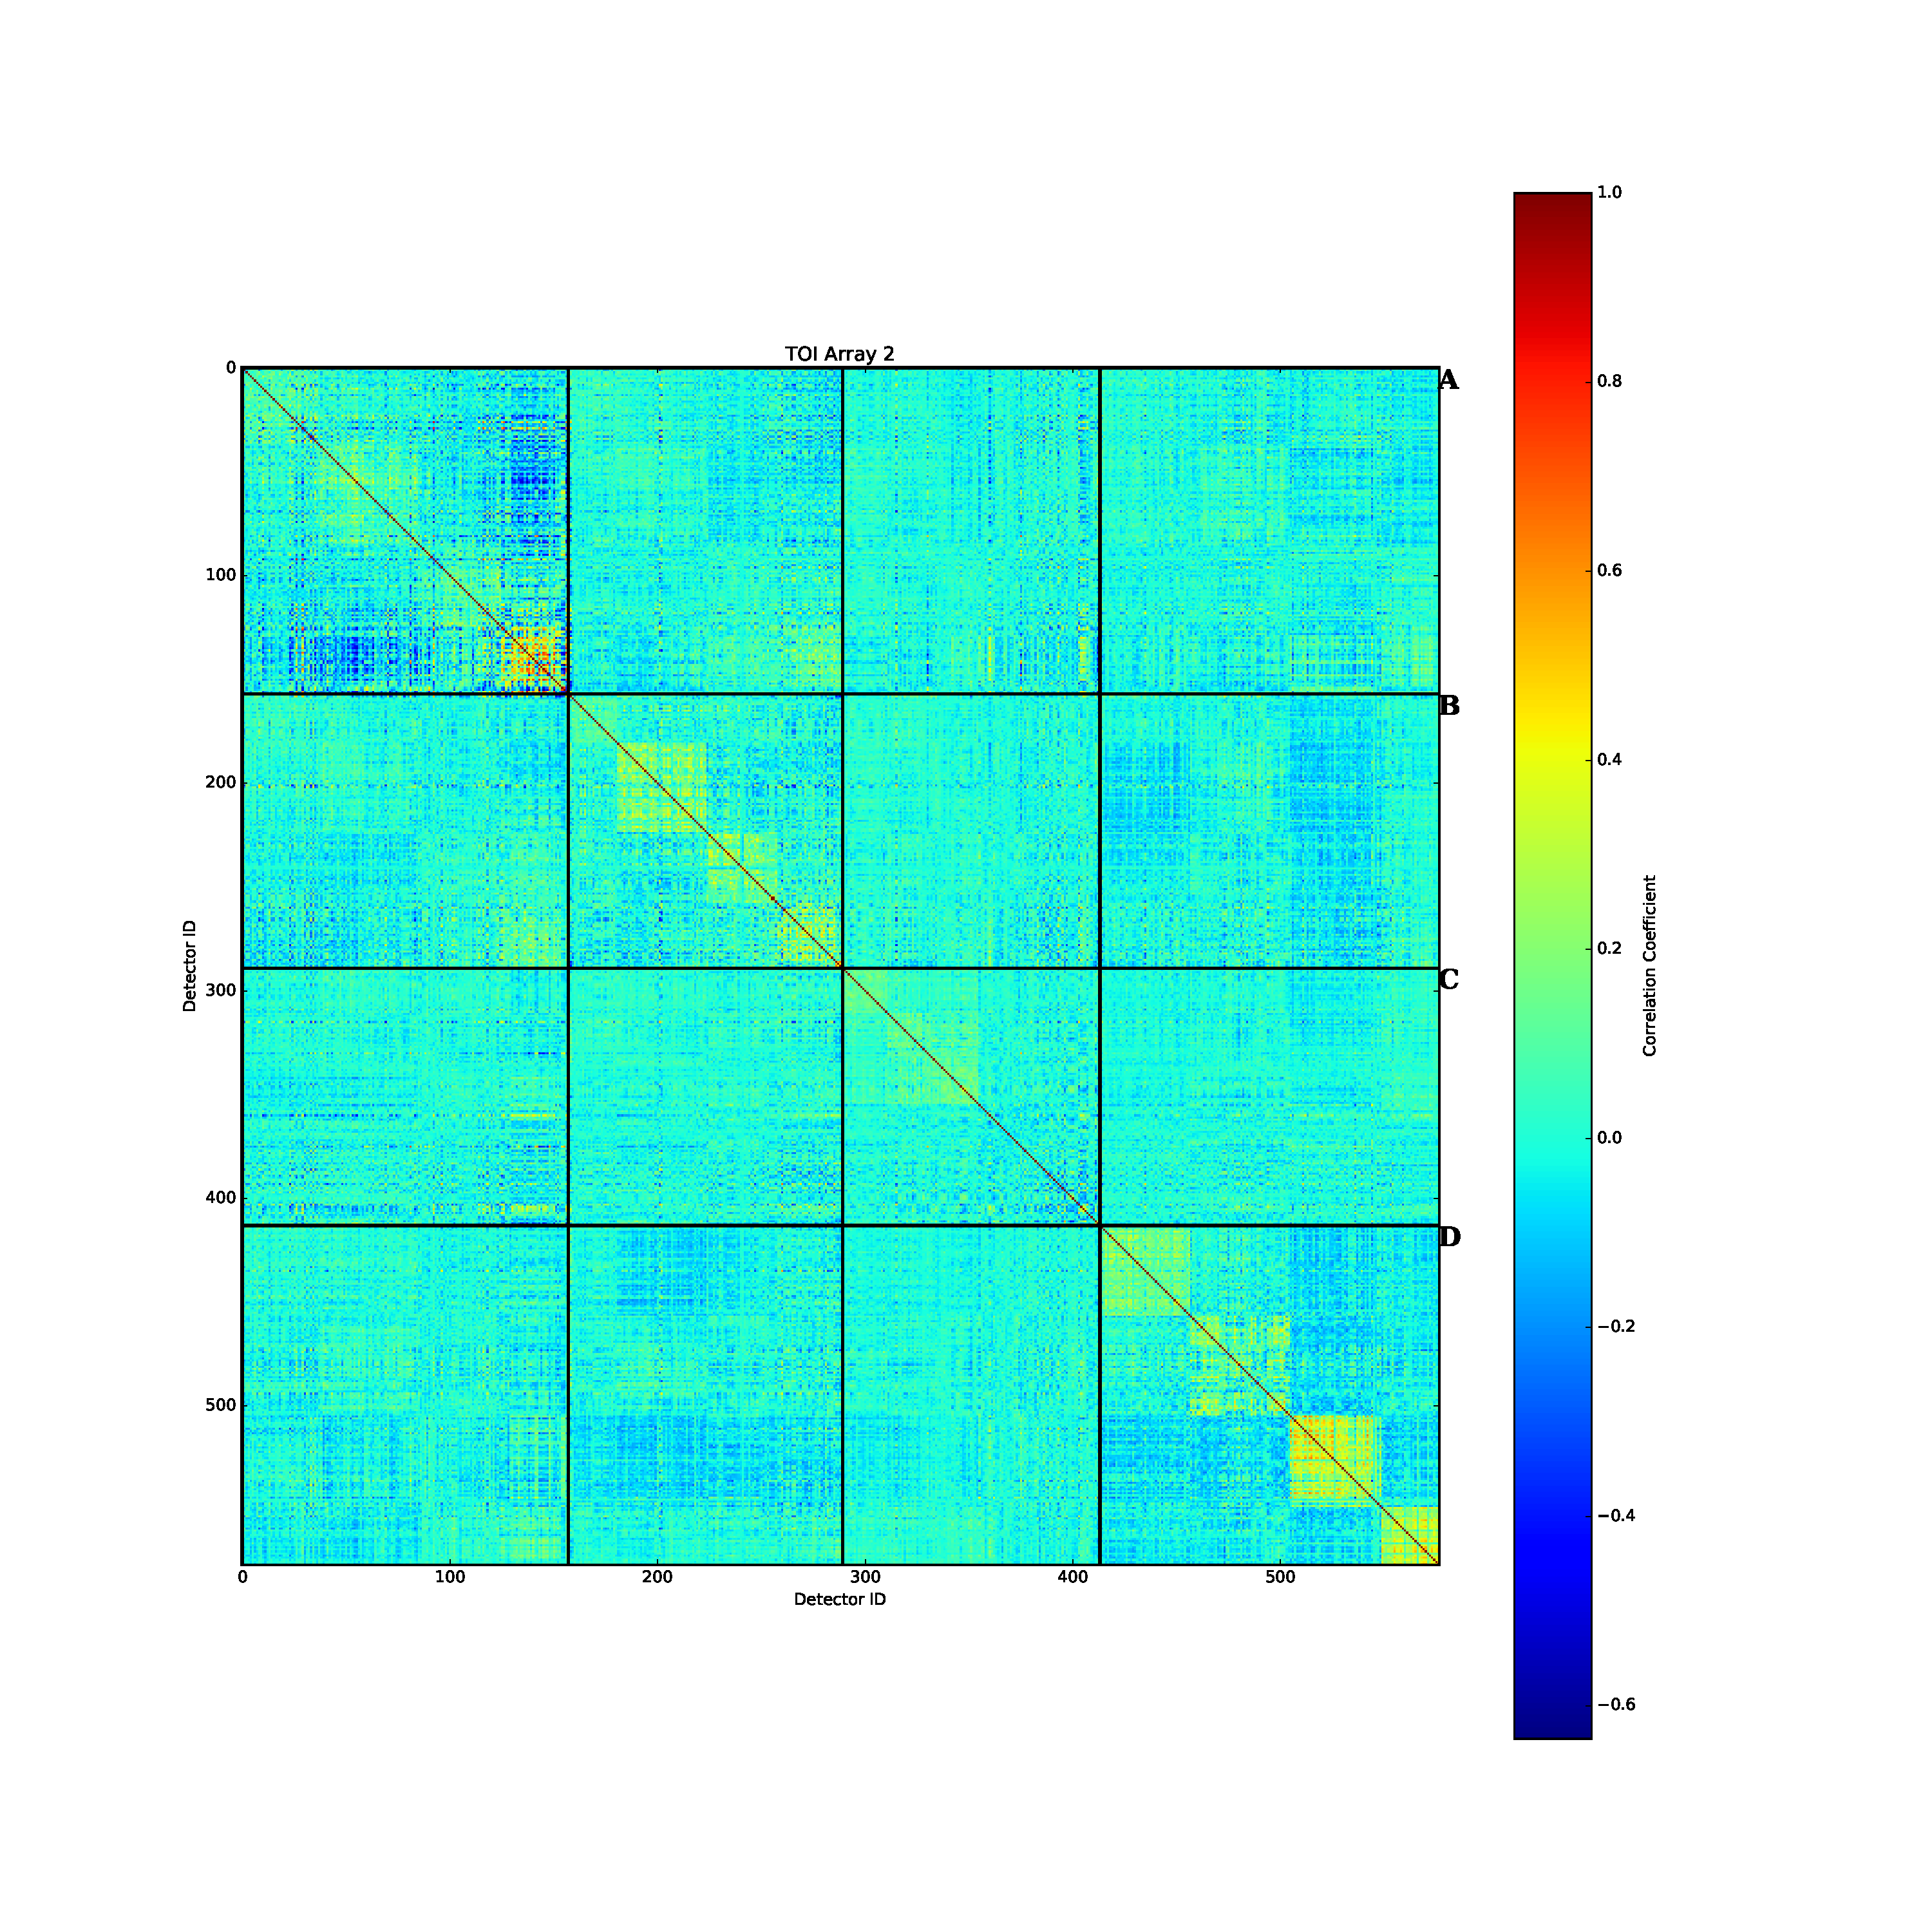
\includegraphics[width=0.3\textwidth]{Figures/DarkTests/corrmat_TOI_BC_array_2_20161211s299.pdf}
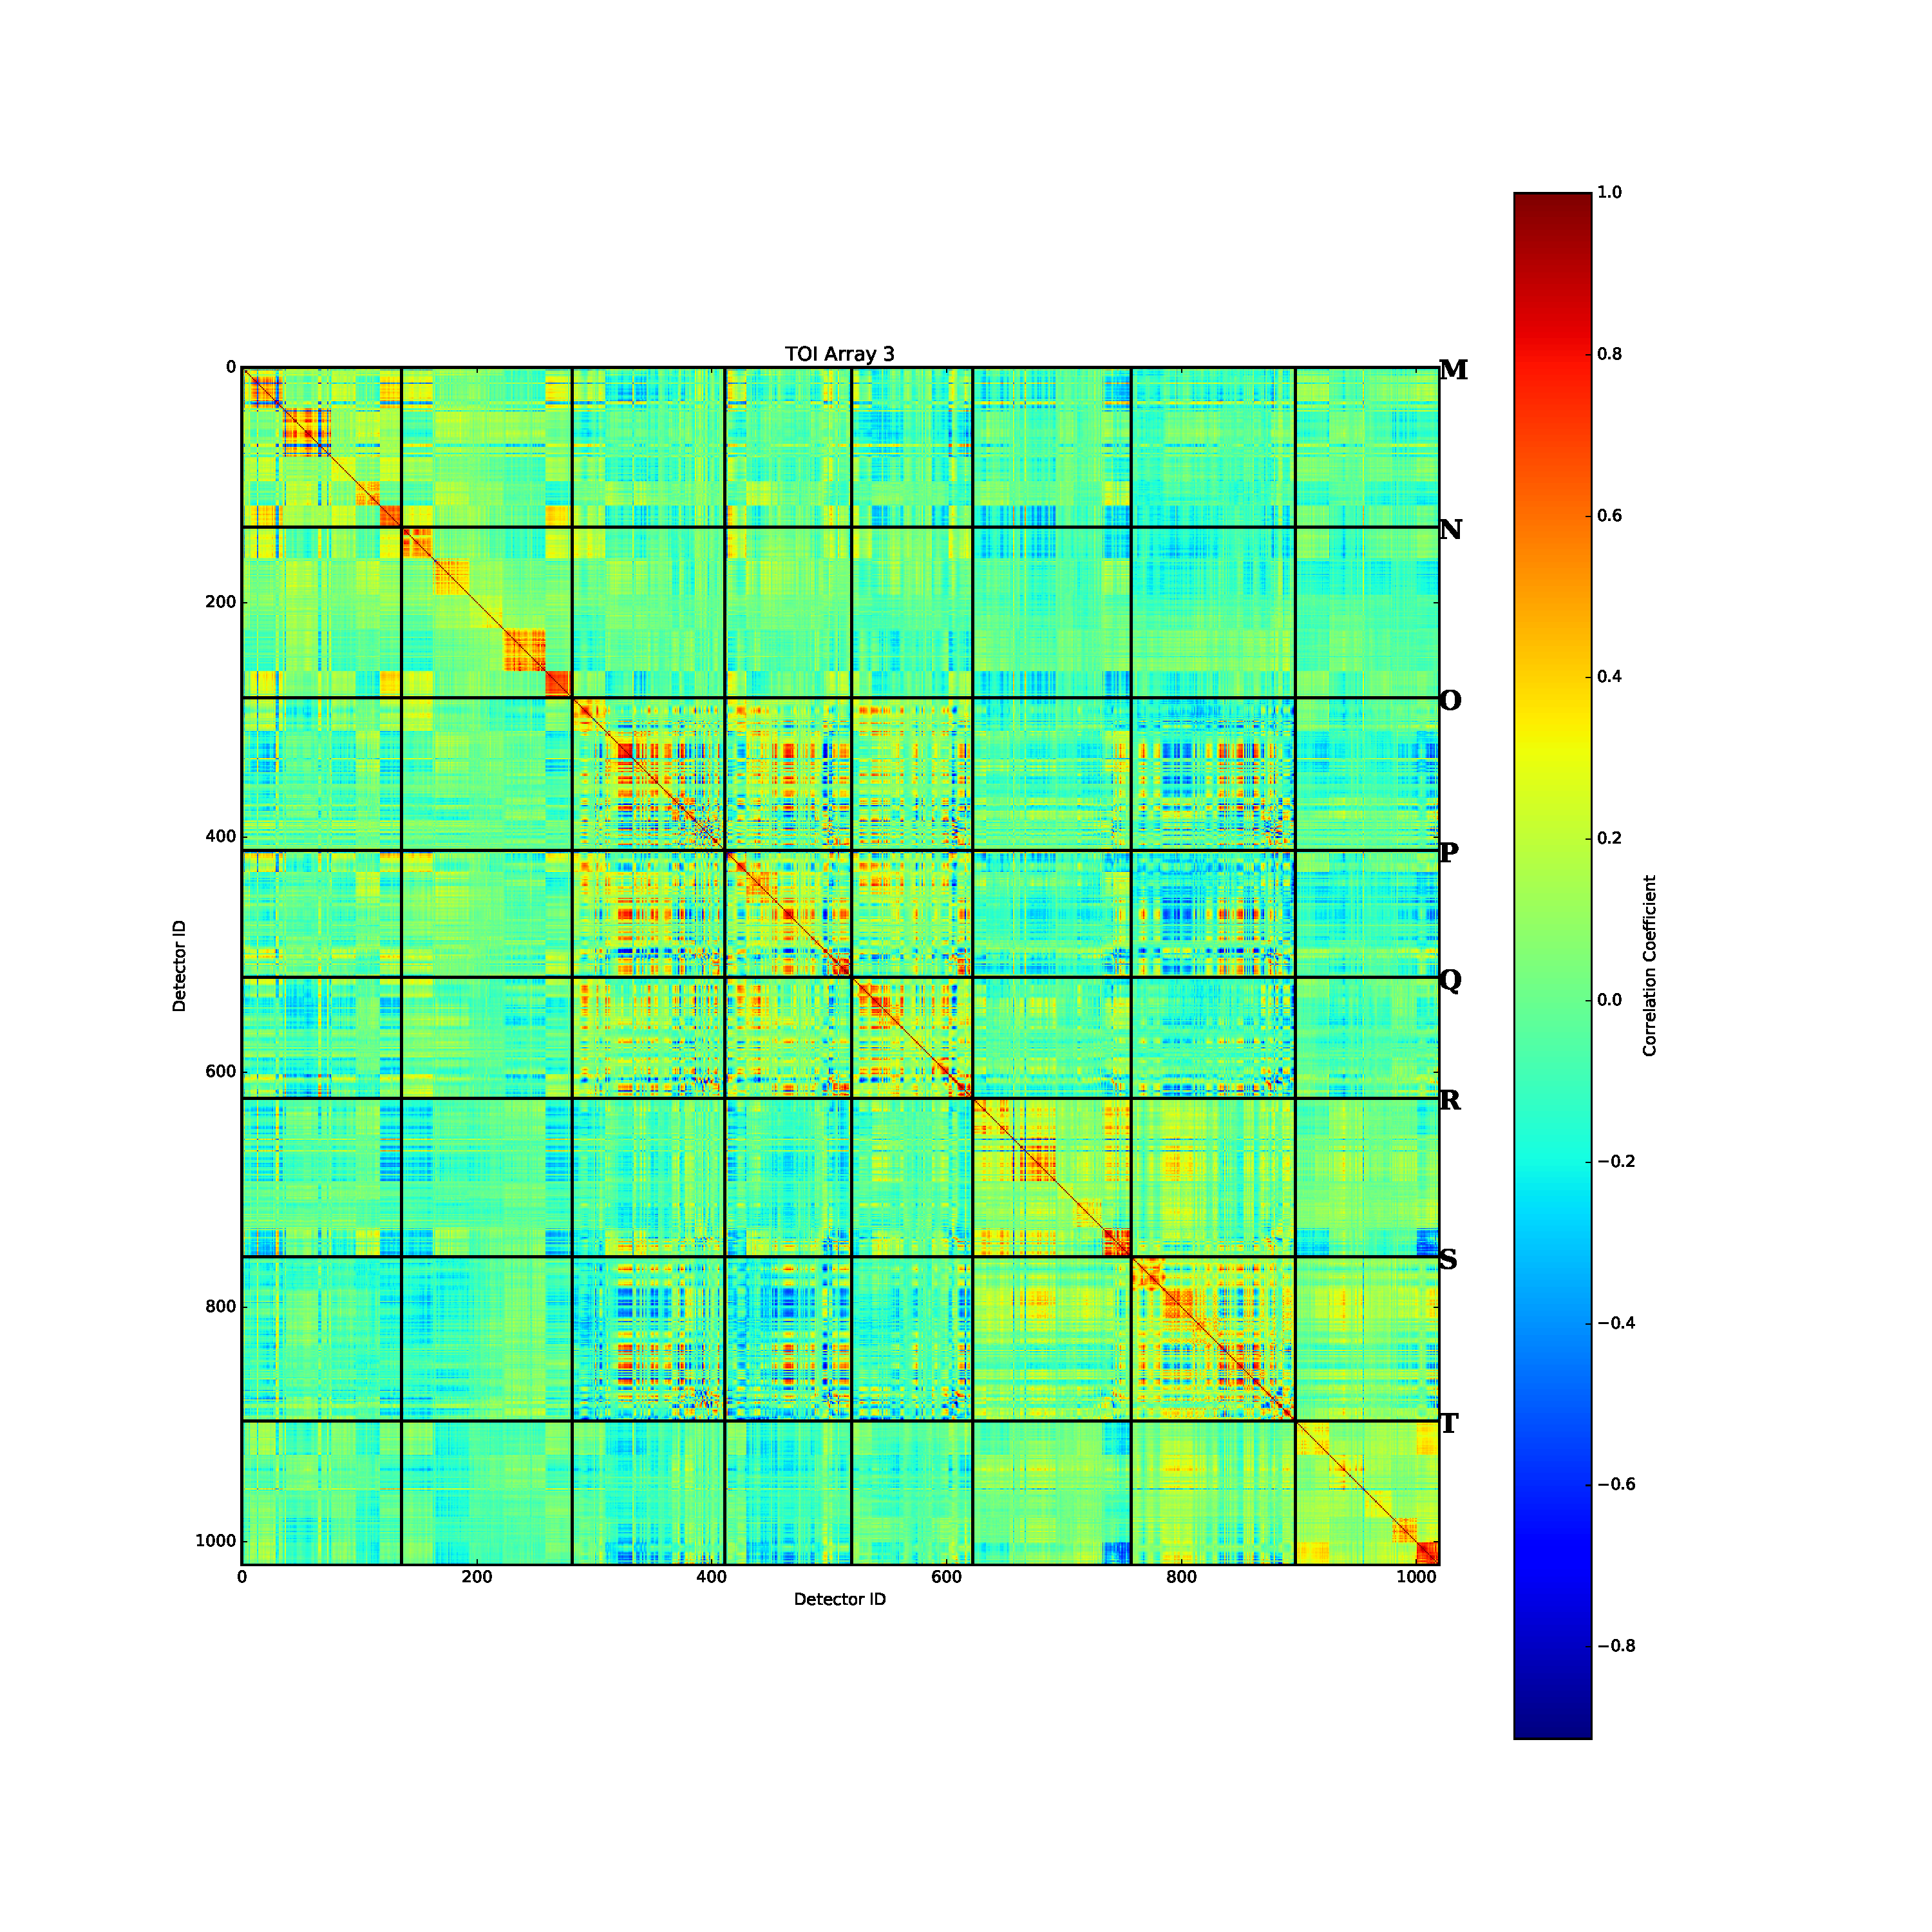
\includegraphics[width=0.3\textwidth]{Figures/DarkTests/corrmat_TOI_BC_array_3_20161211s299.pdf}
\end{center}
\caption{From left to right correlation matrices for the three NIKA2 arrays (A1, A2, and A3) for scan 20161211s299. From top to bottom we present the correlation of the raw data, after CM, PCA and BC decorrelations. \label{corrs299}}
\end{figure}



\begin{figure}[ht] % Inline image example
\begin{center}
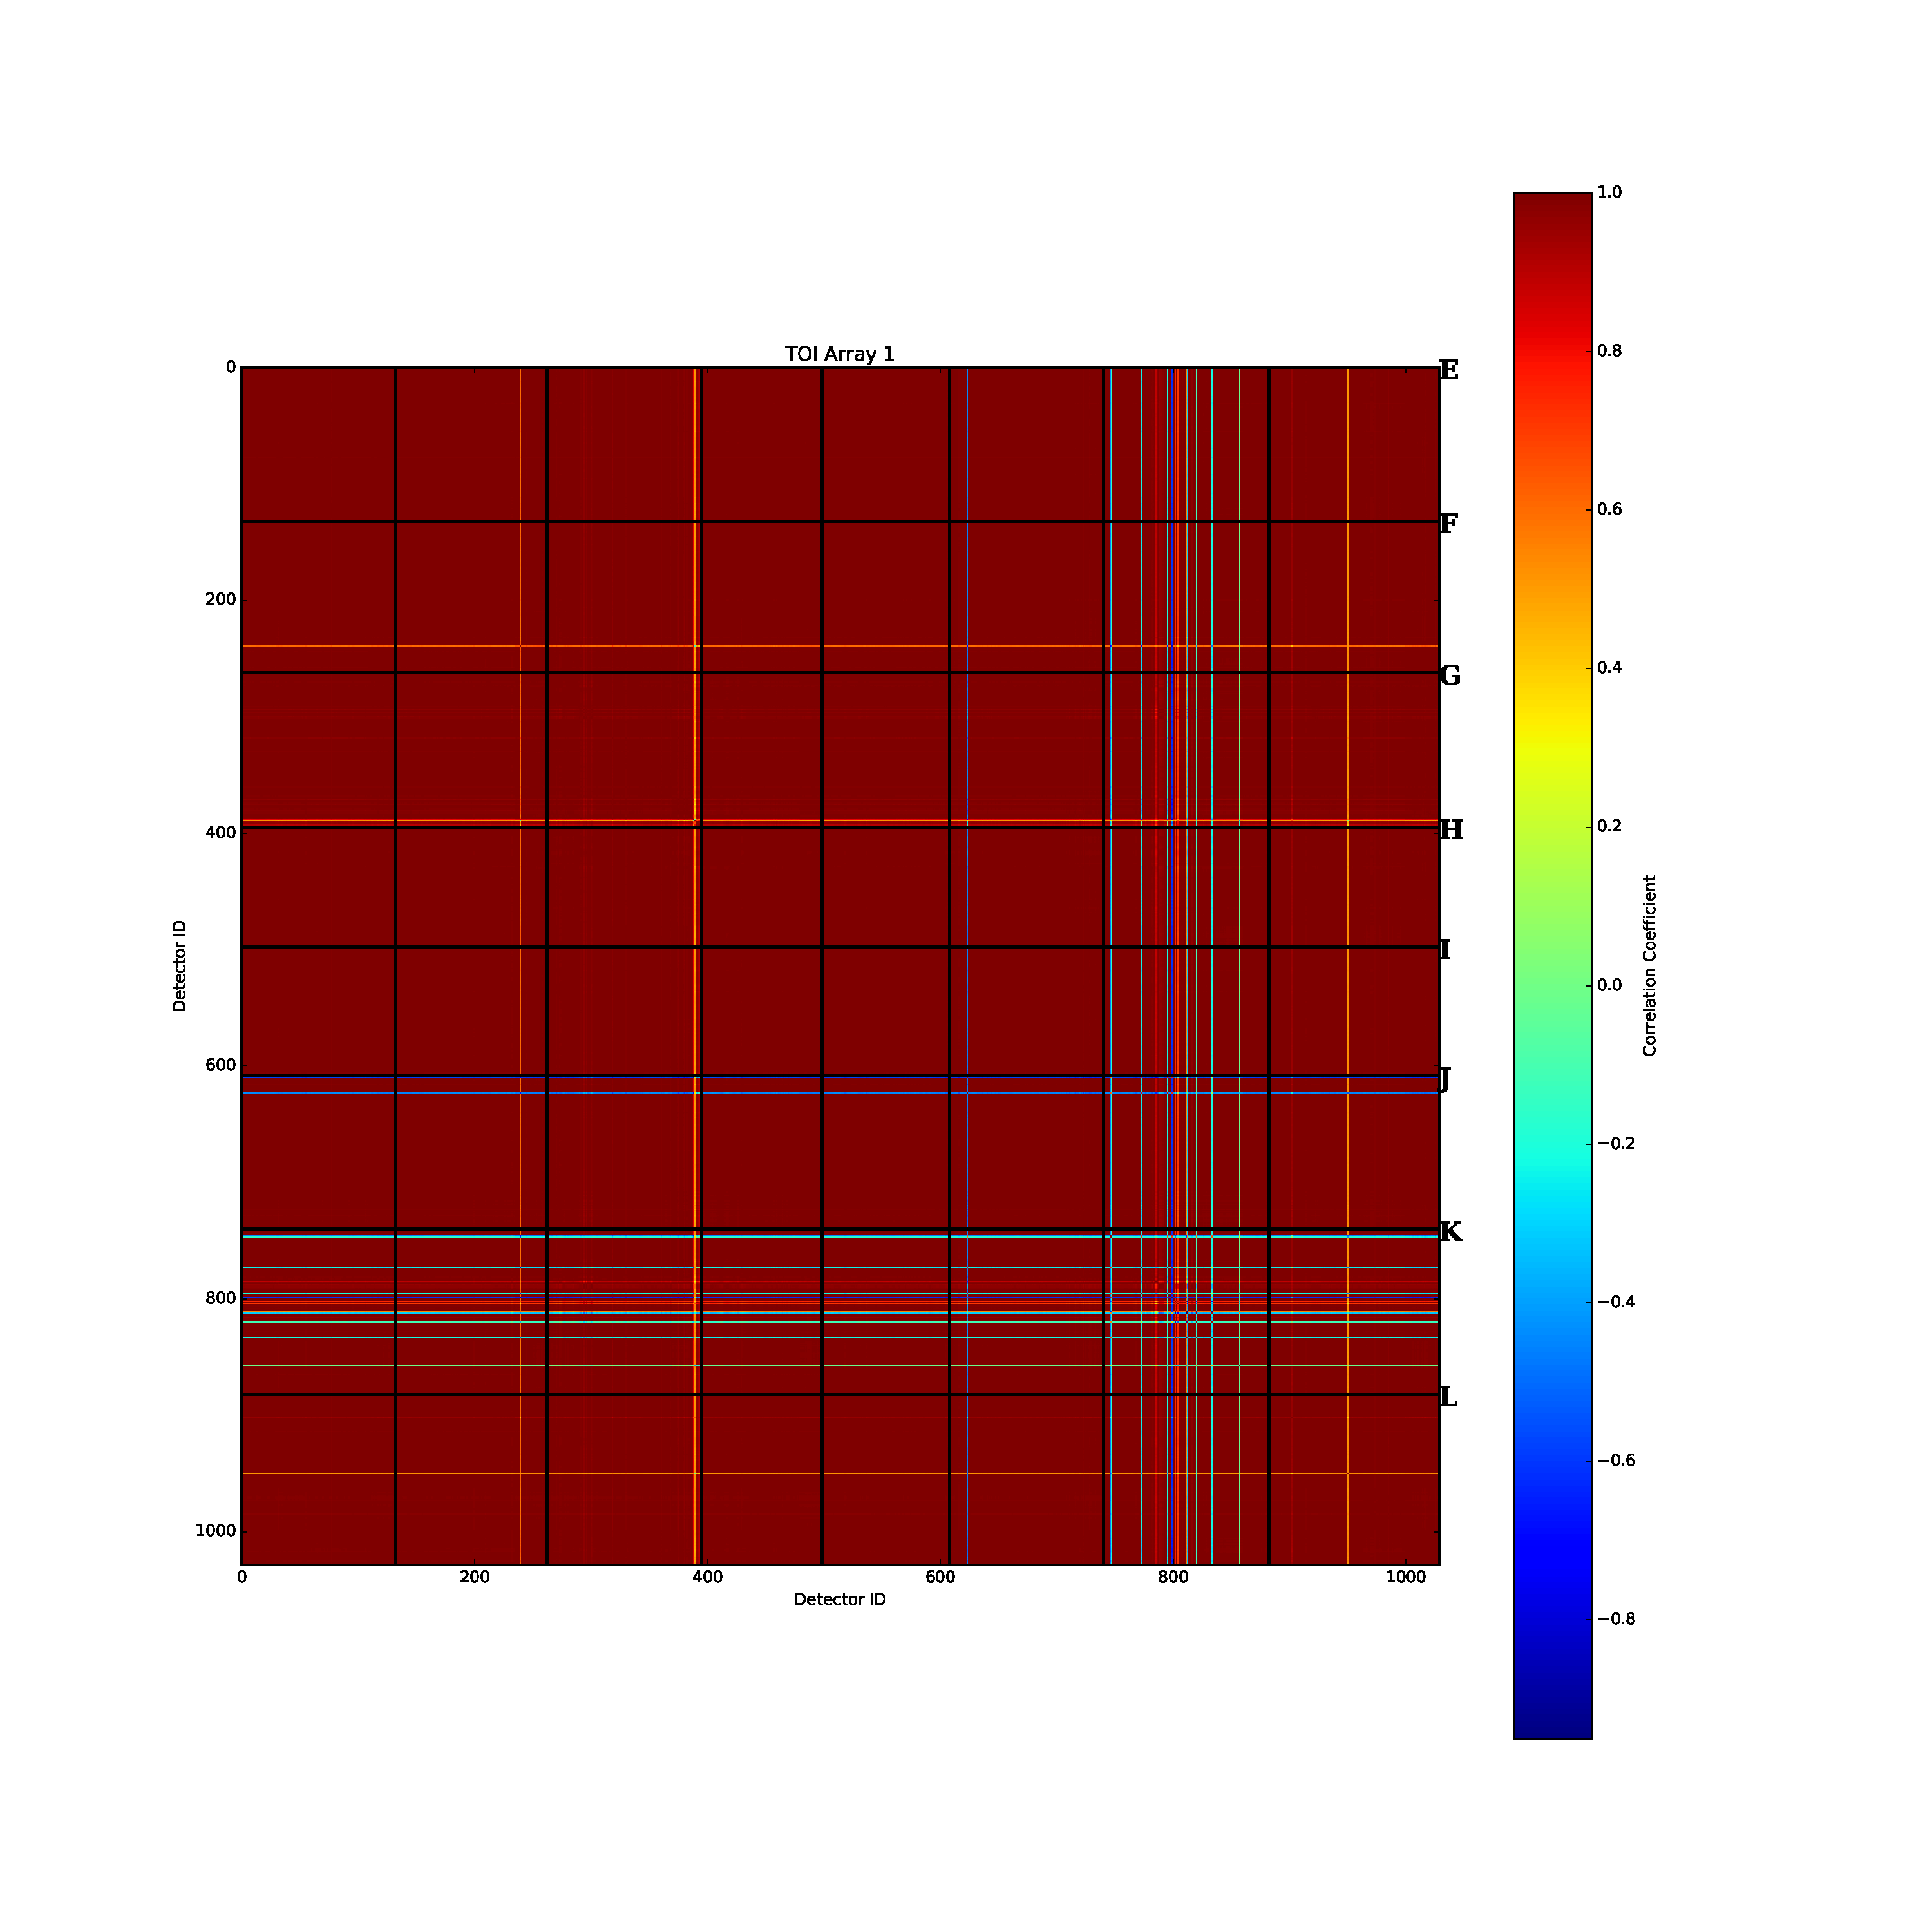
\includegraphics[width=0.3\textwidth]{Figures/DarkTests/corrmat_TOI_array_1_20161213s72.pdf}
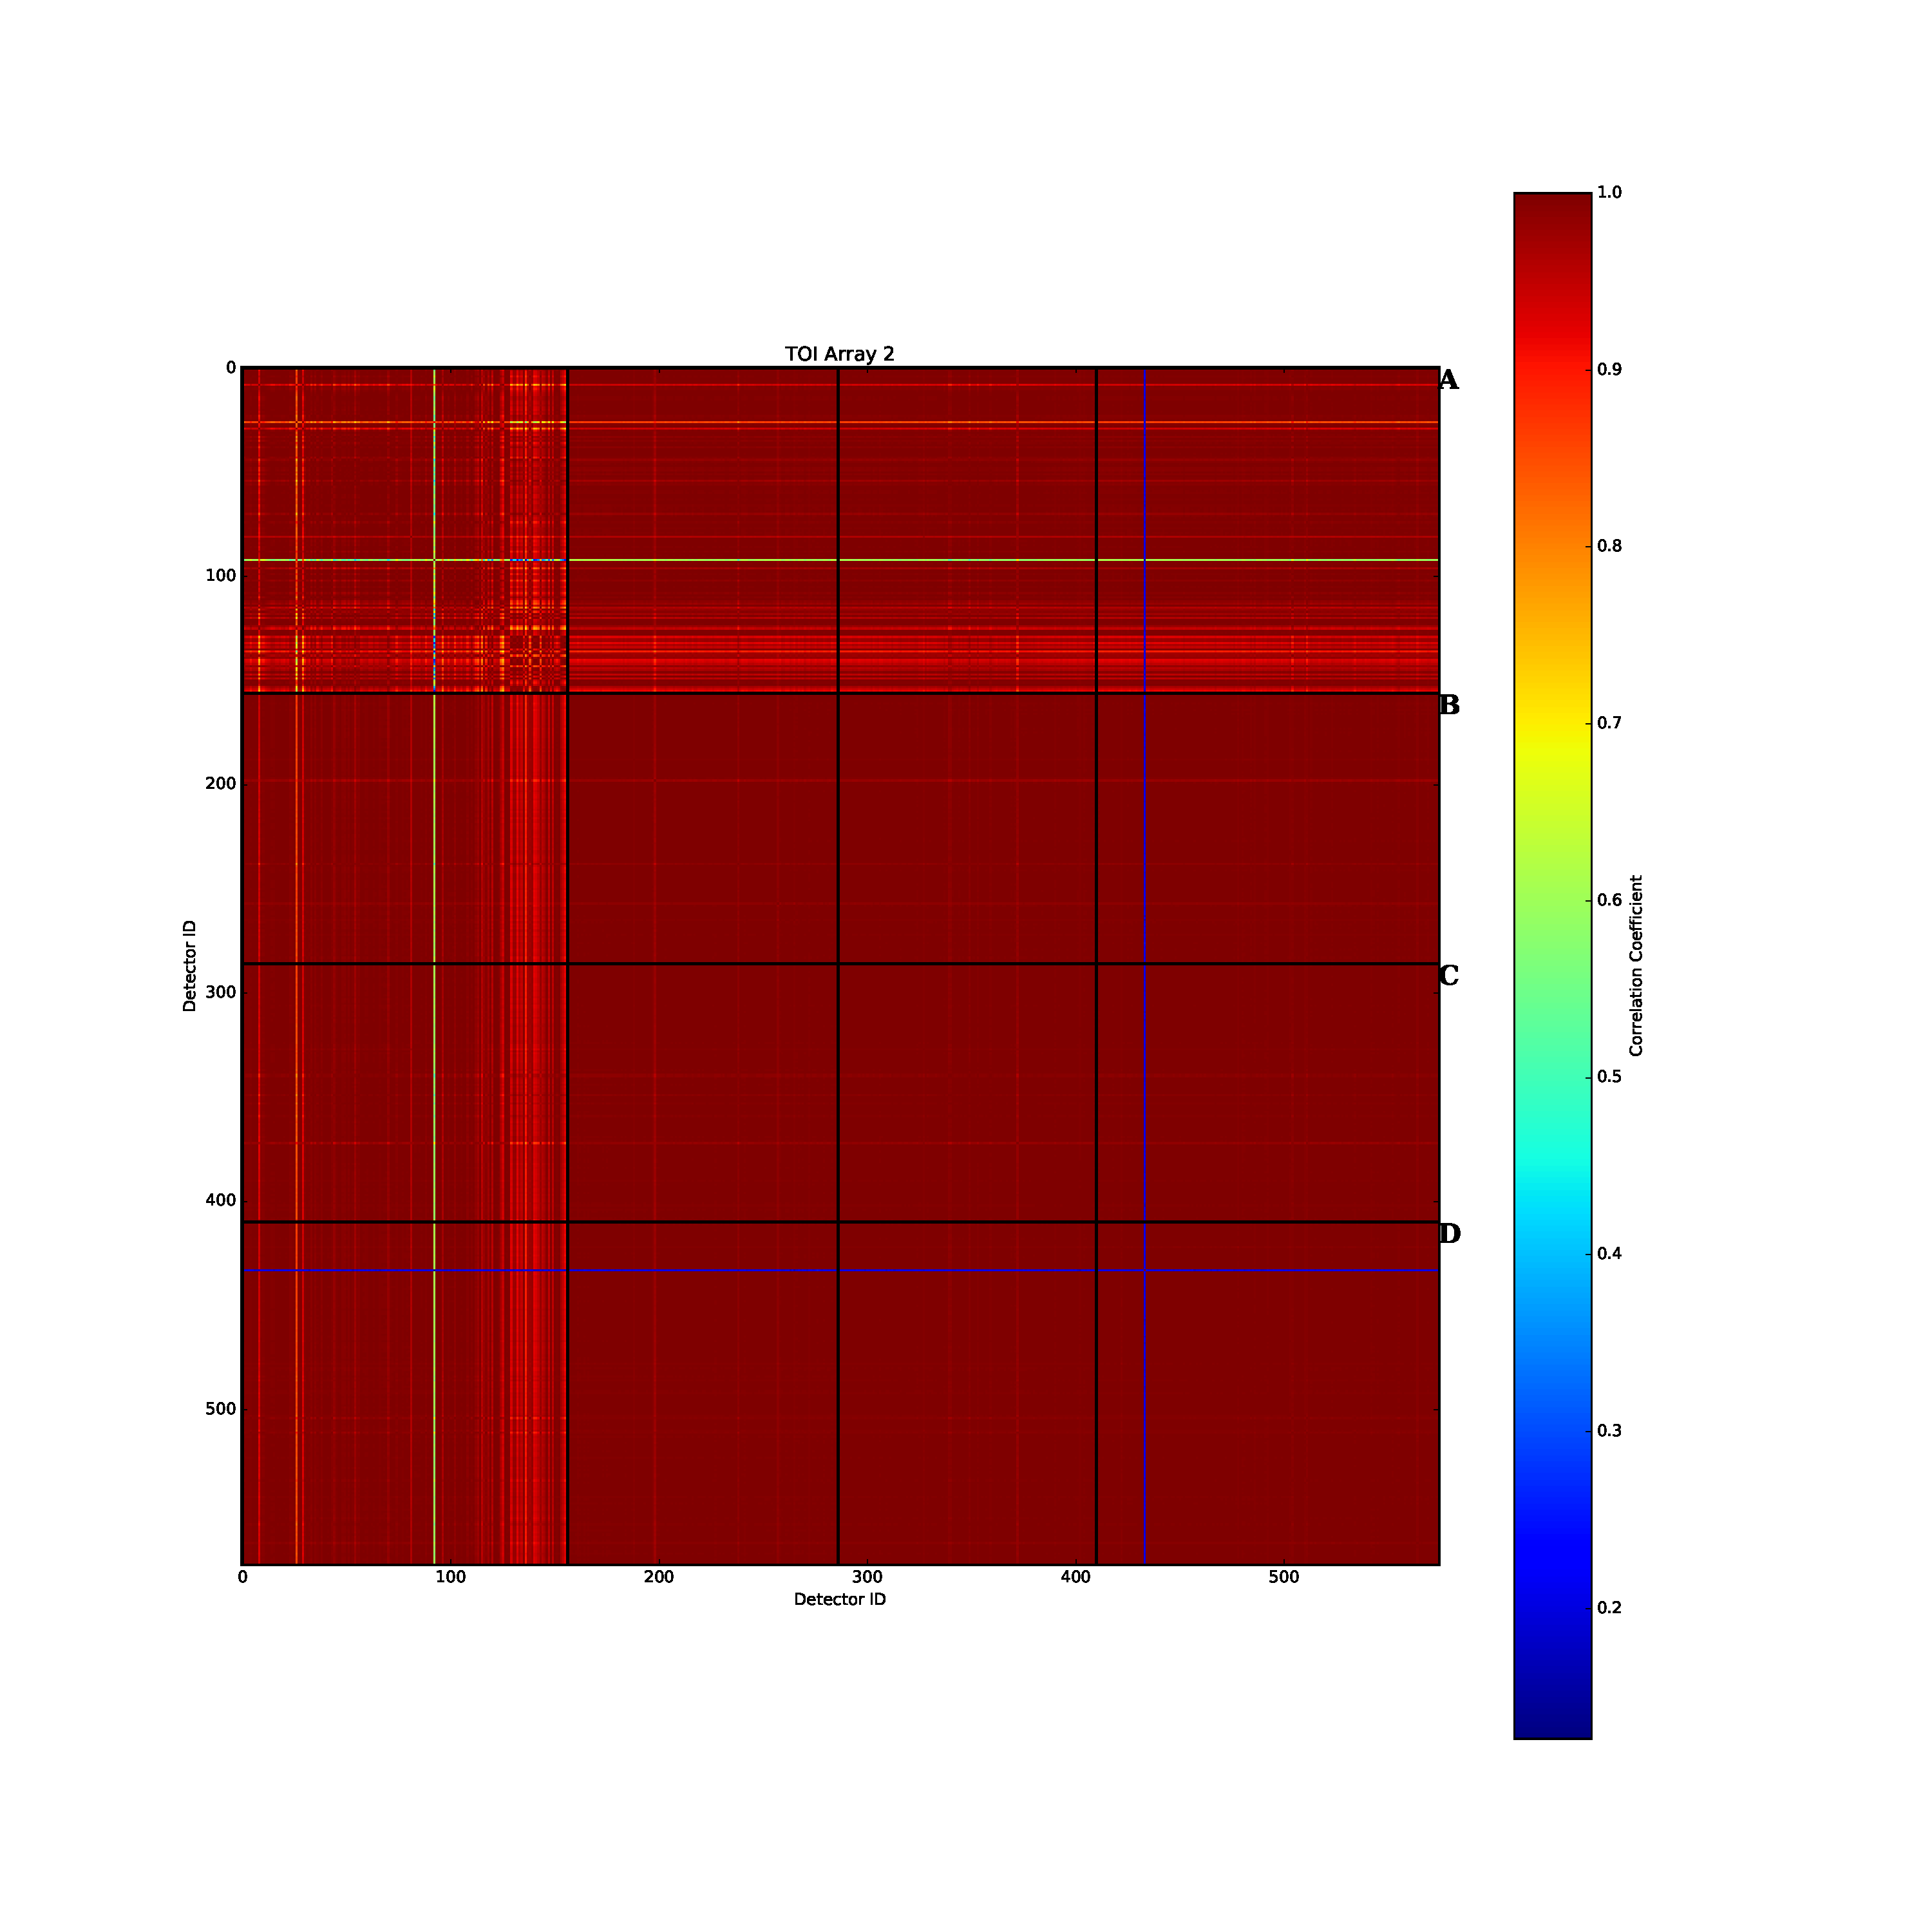
\includegraphics[width=0.3\textwidth]{Figures/DarkTests/corrmat_TOI_array_2_20161213s72.pdf}
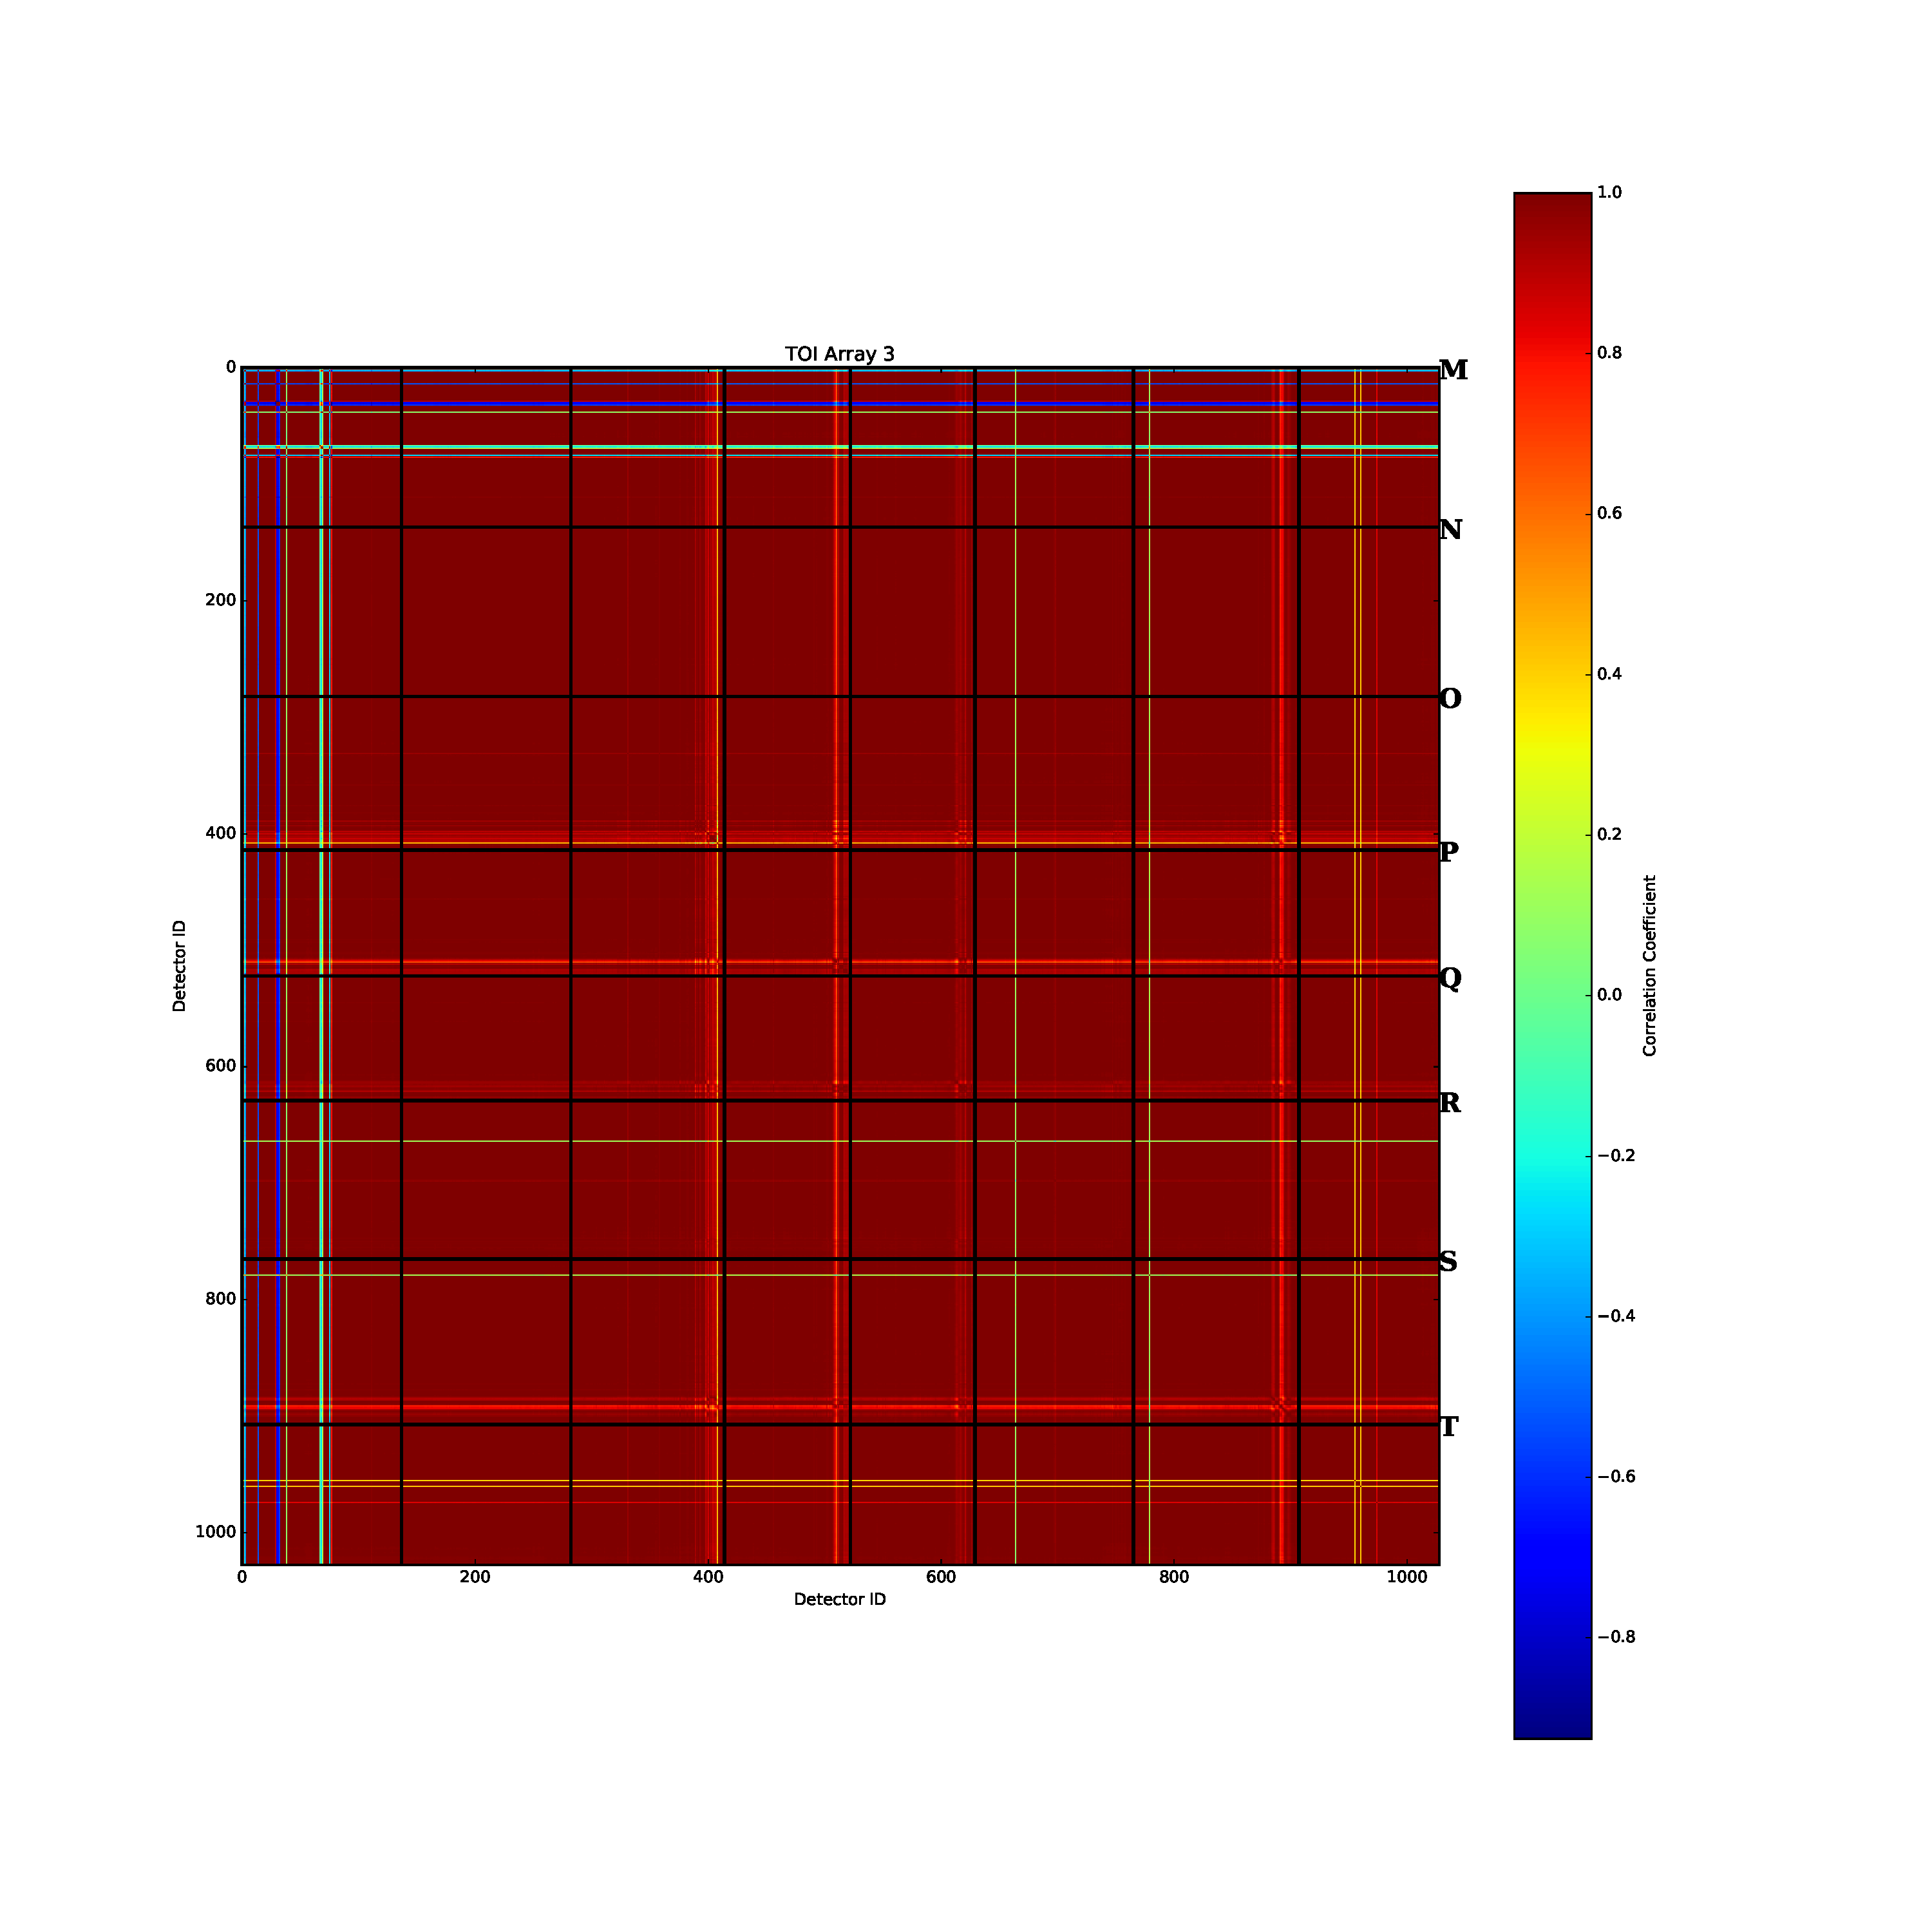
\includegraphics[width=0.3\textwidth]{Figures/DarkTests/corrmat_TOI_array_3_20161213s72.pdf}
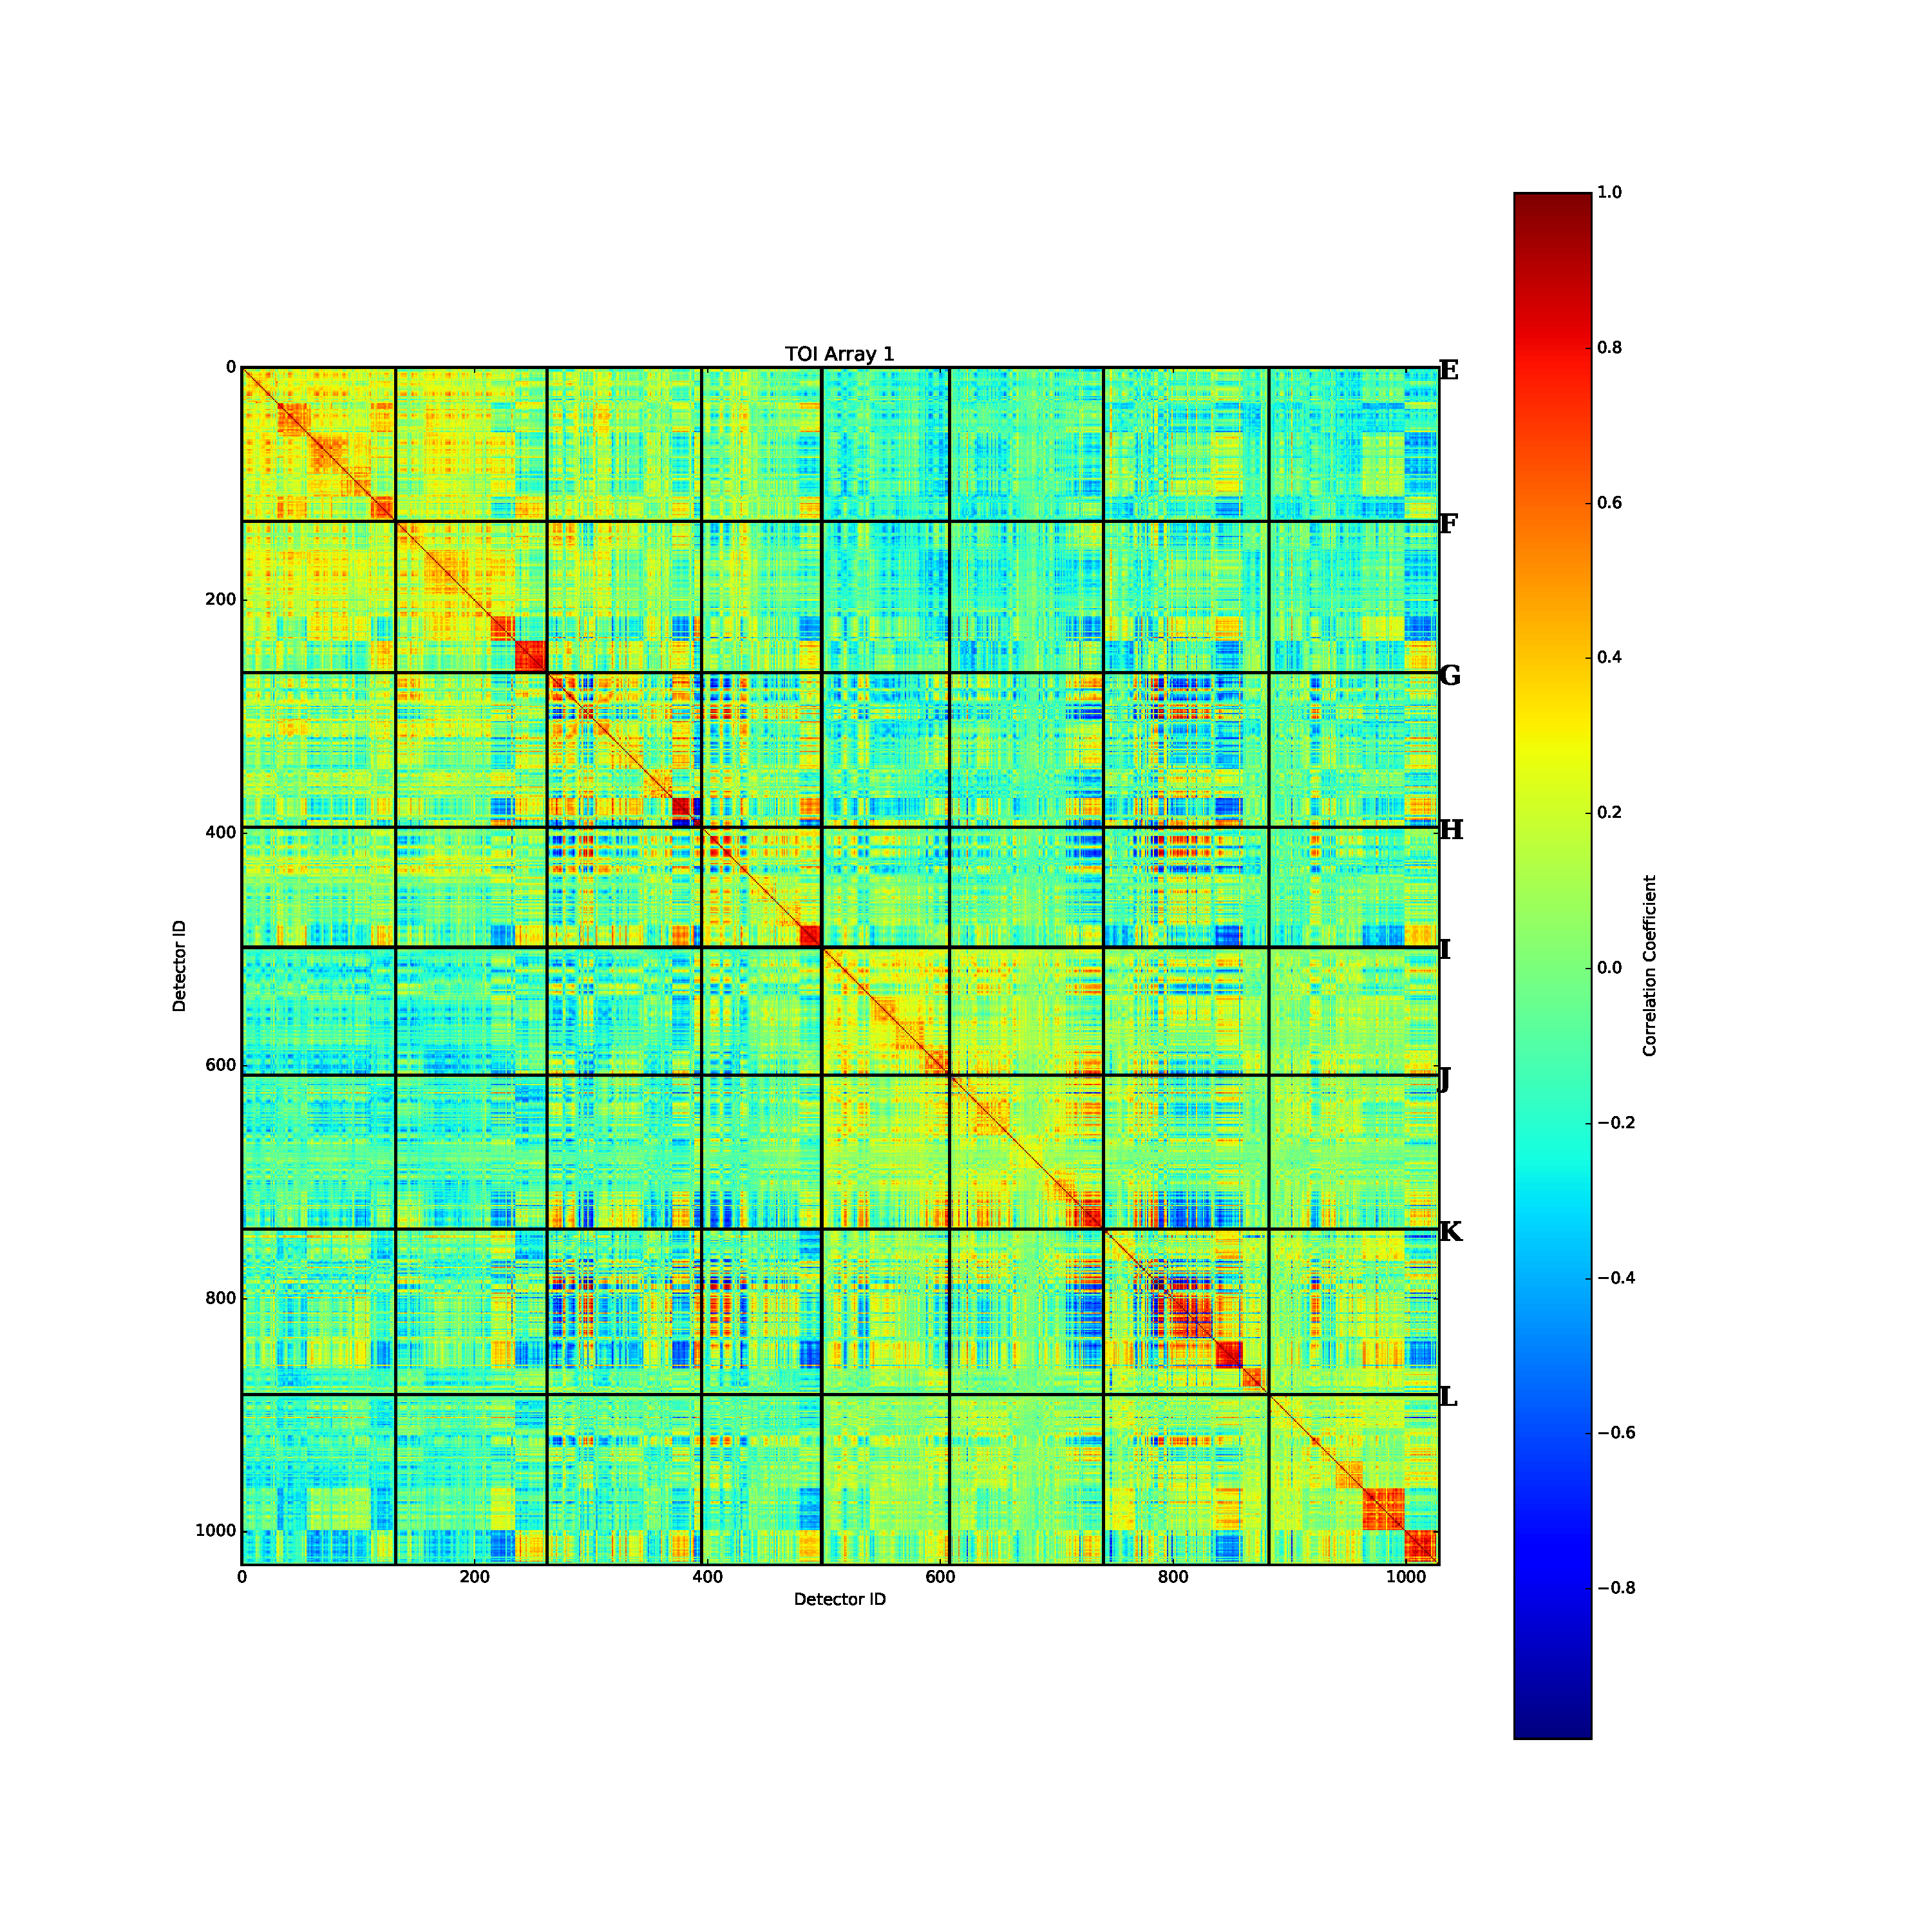
\includegraphics[width=0.3\textwidth]{Figures/DarkTests/corrmat_TOI_CM_array_1_20161213s72.pdf}
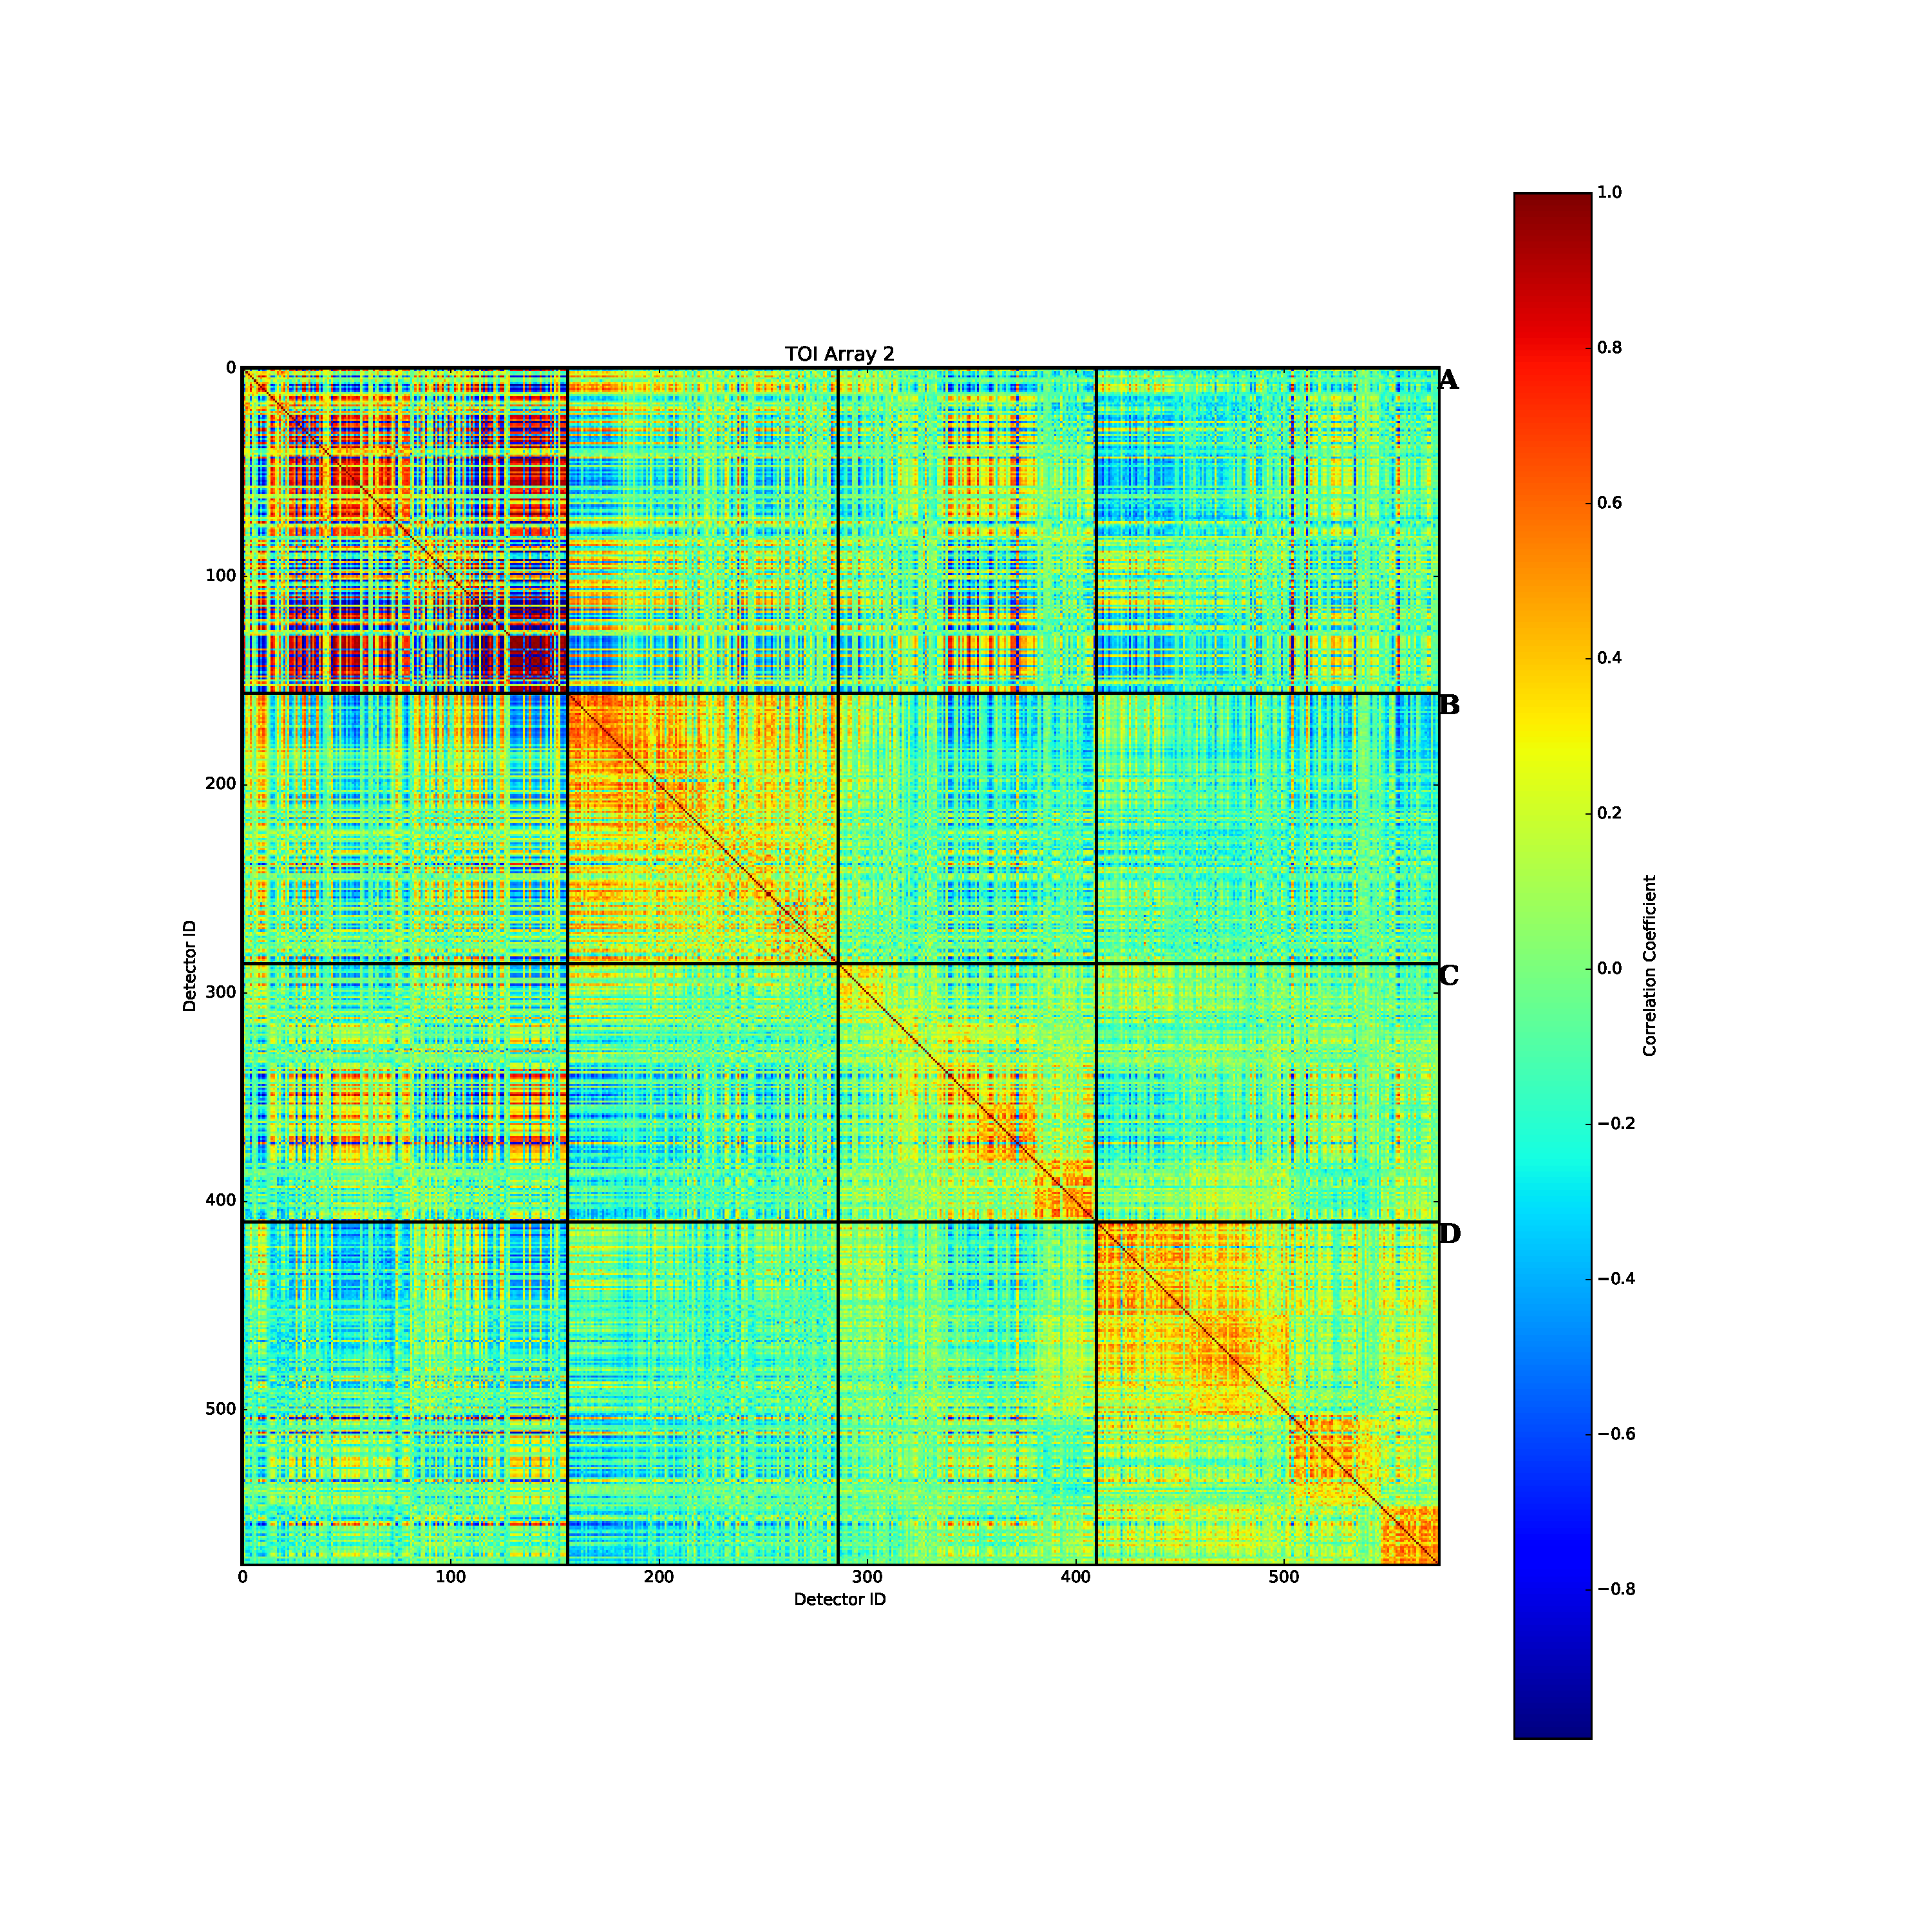
\includegraphics[width=0.3\textwidth]{Figures/DarkTests/corrmat_TOI_CM_array_2_20161213s72.pdf}
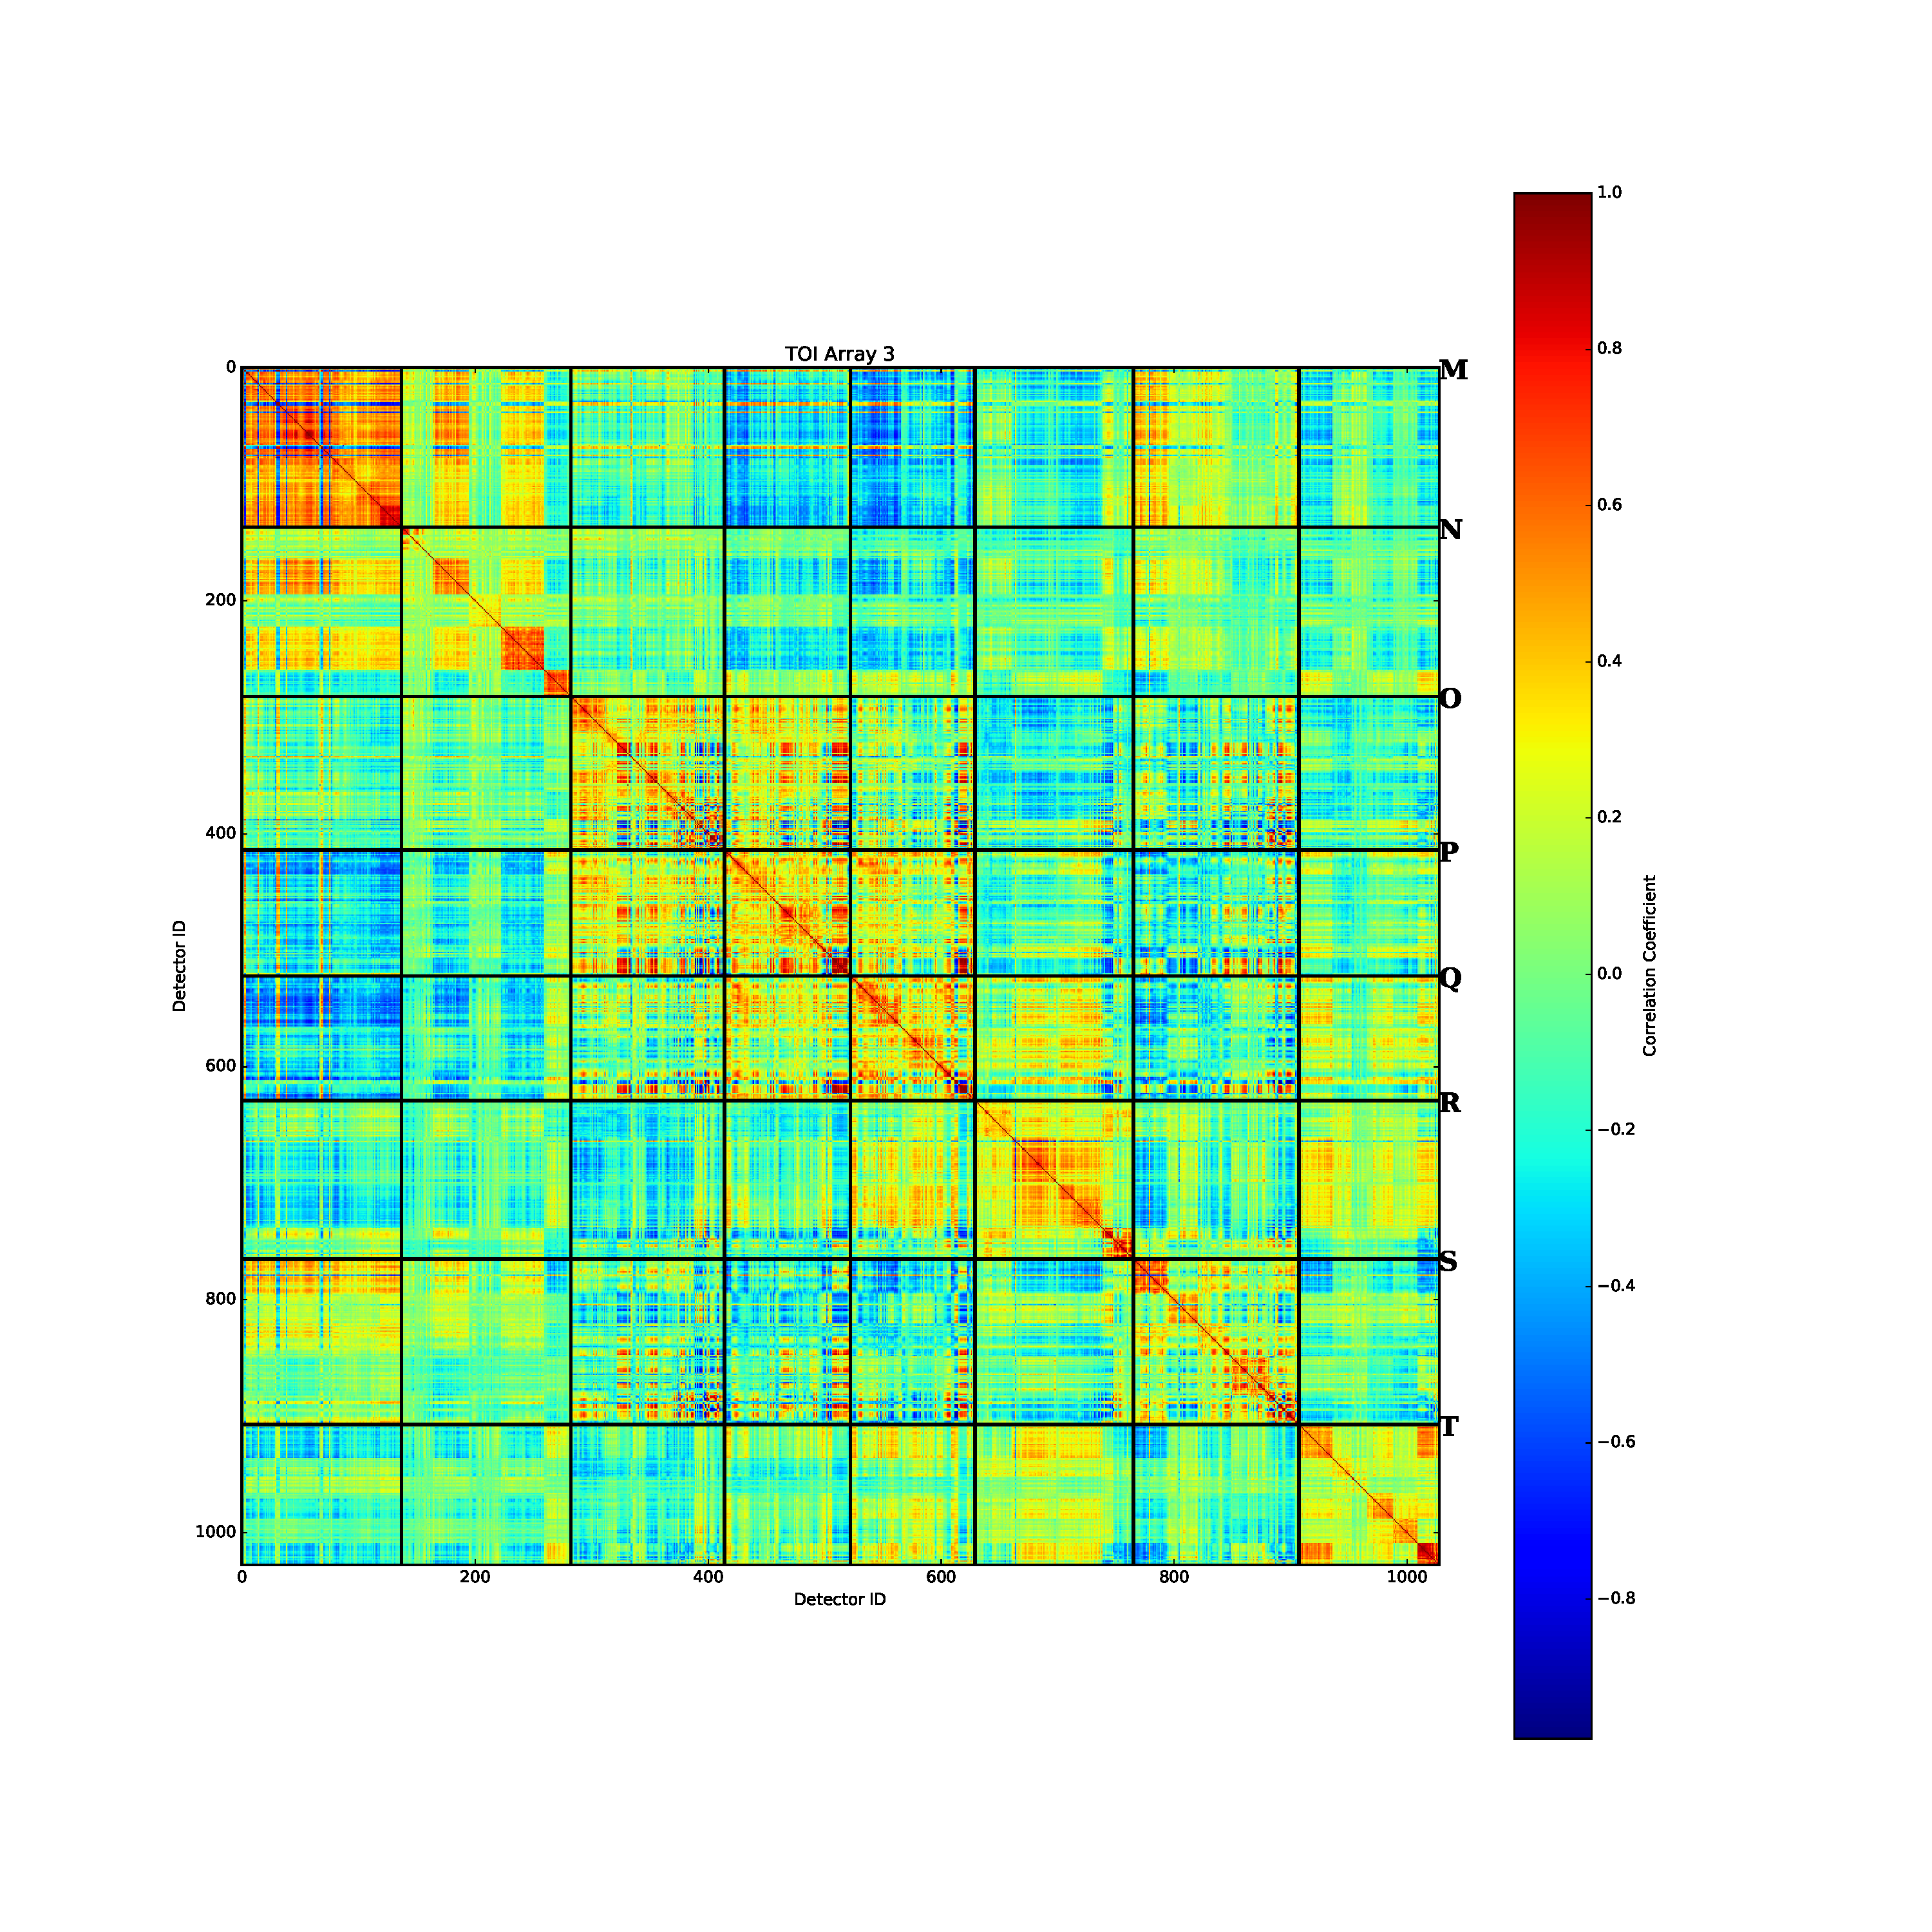
\includegraphics[width=0.3\textwidth]{Figures/DarkTests/corrmat_TOI_CM_array_3_20161213s72.pdf}
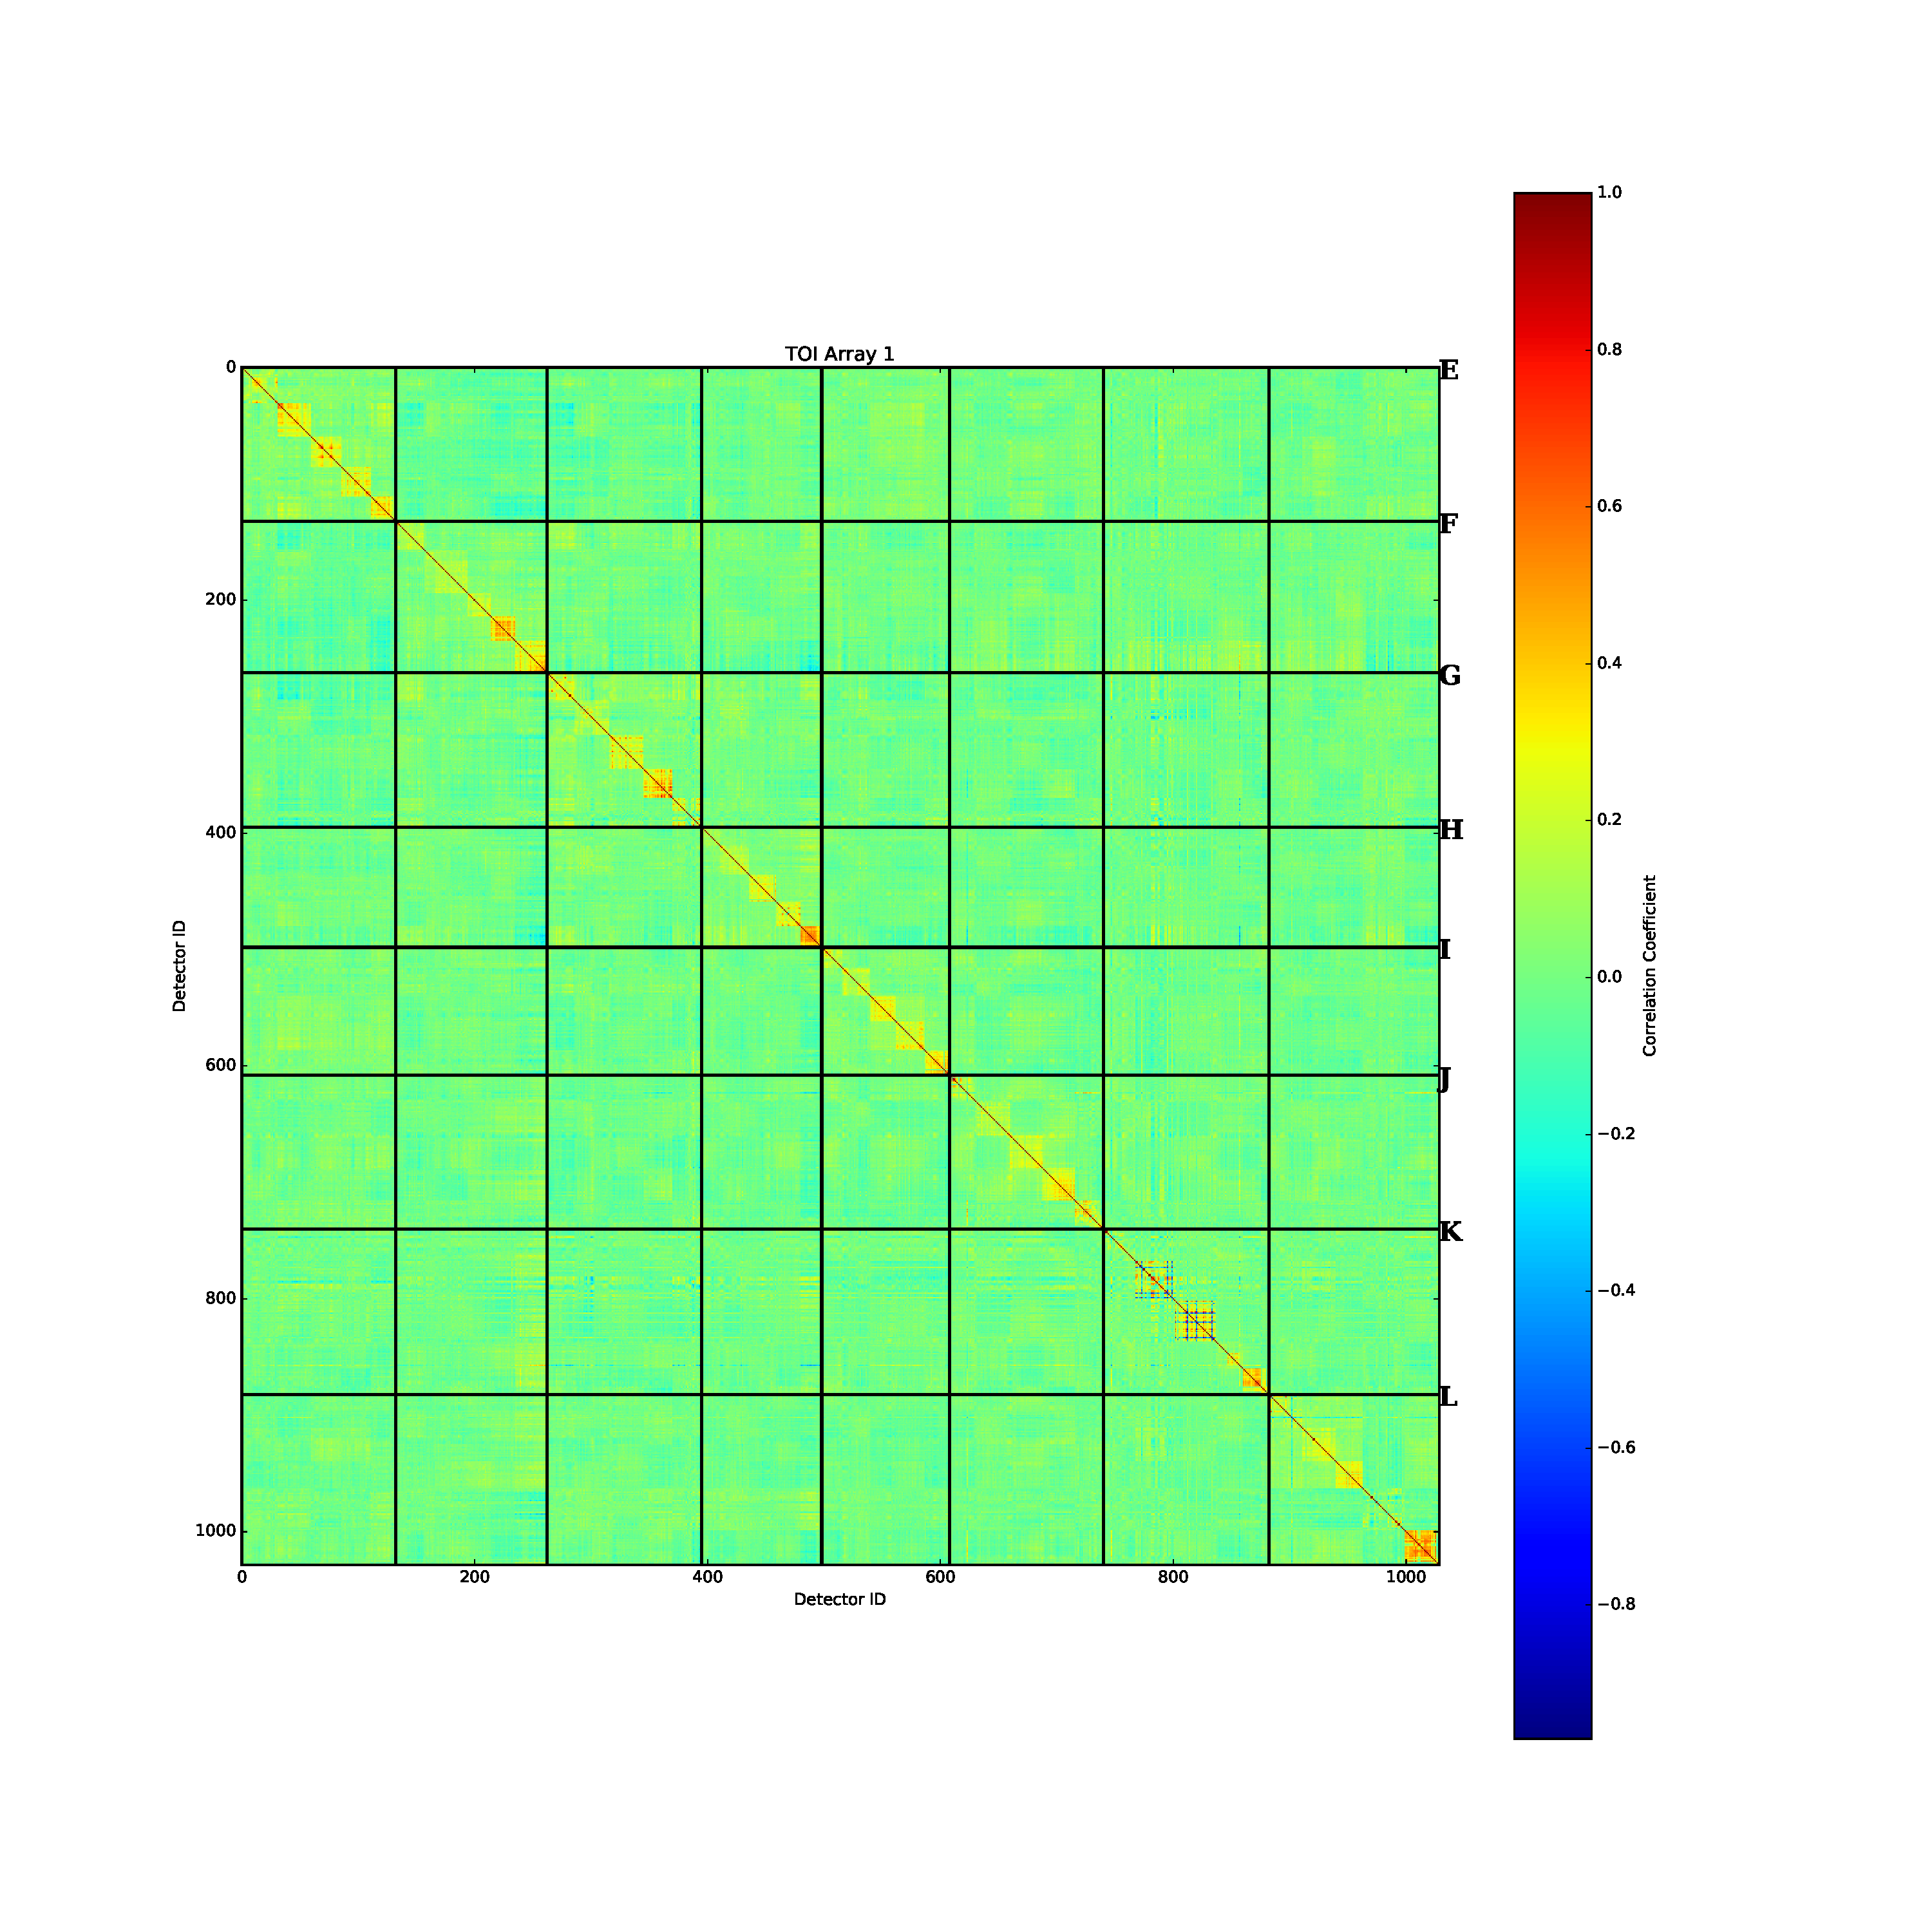
\includegraphics[width=0.3\textwidth]{Figures/DarkTests/corrmat_TOI_PCA_array_1_20161213s72.pdf}
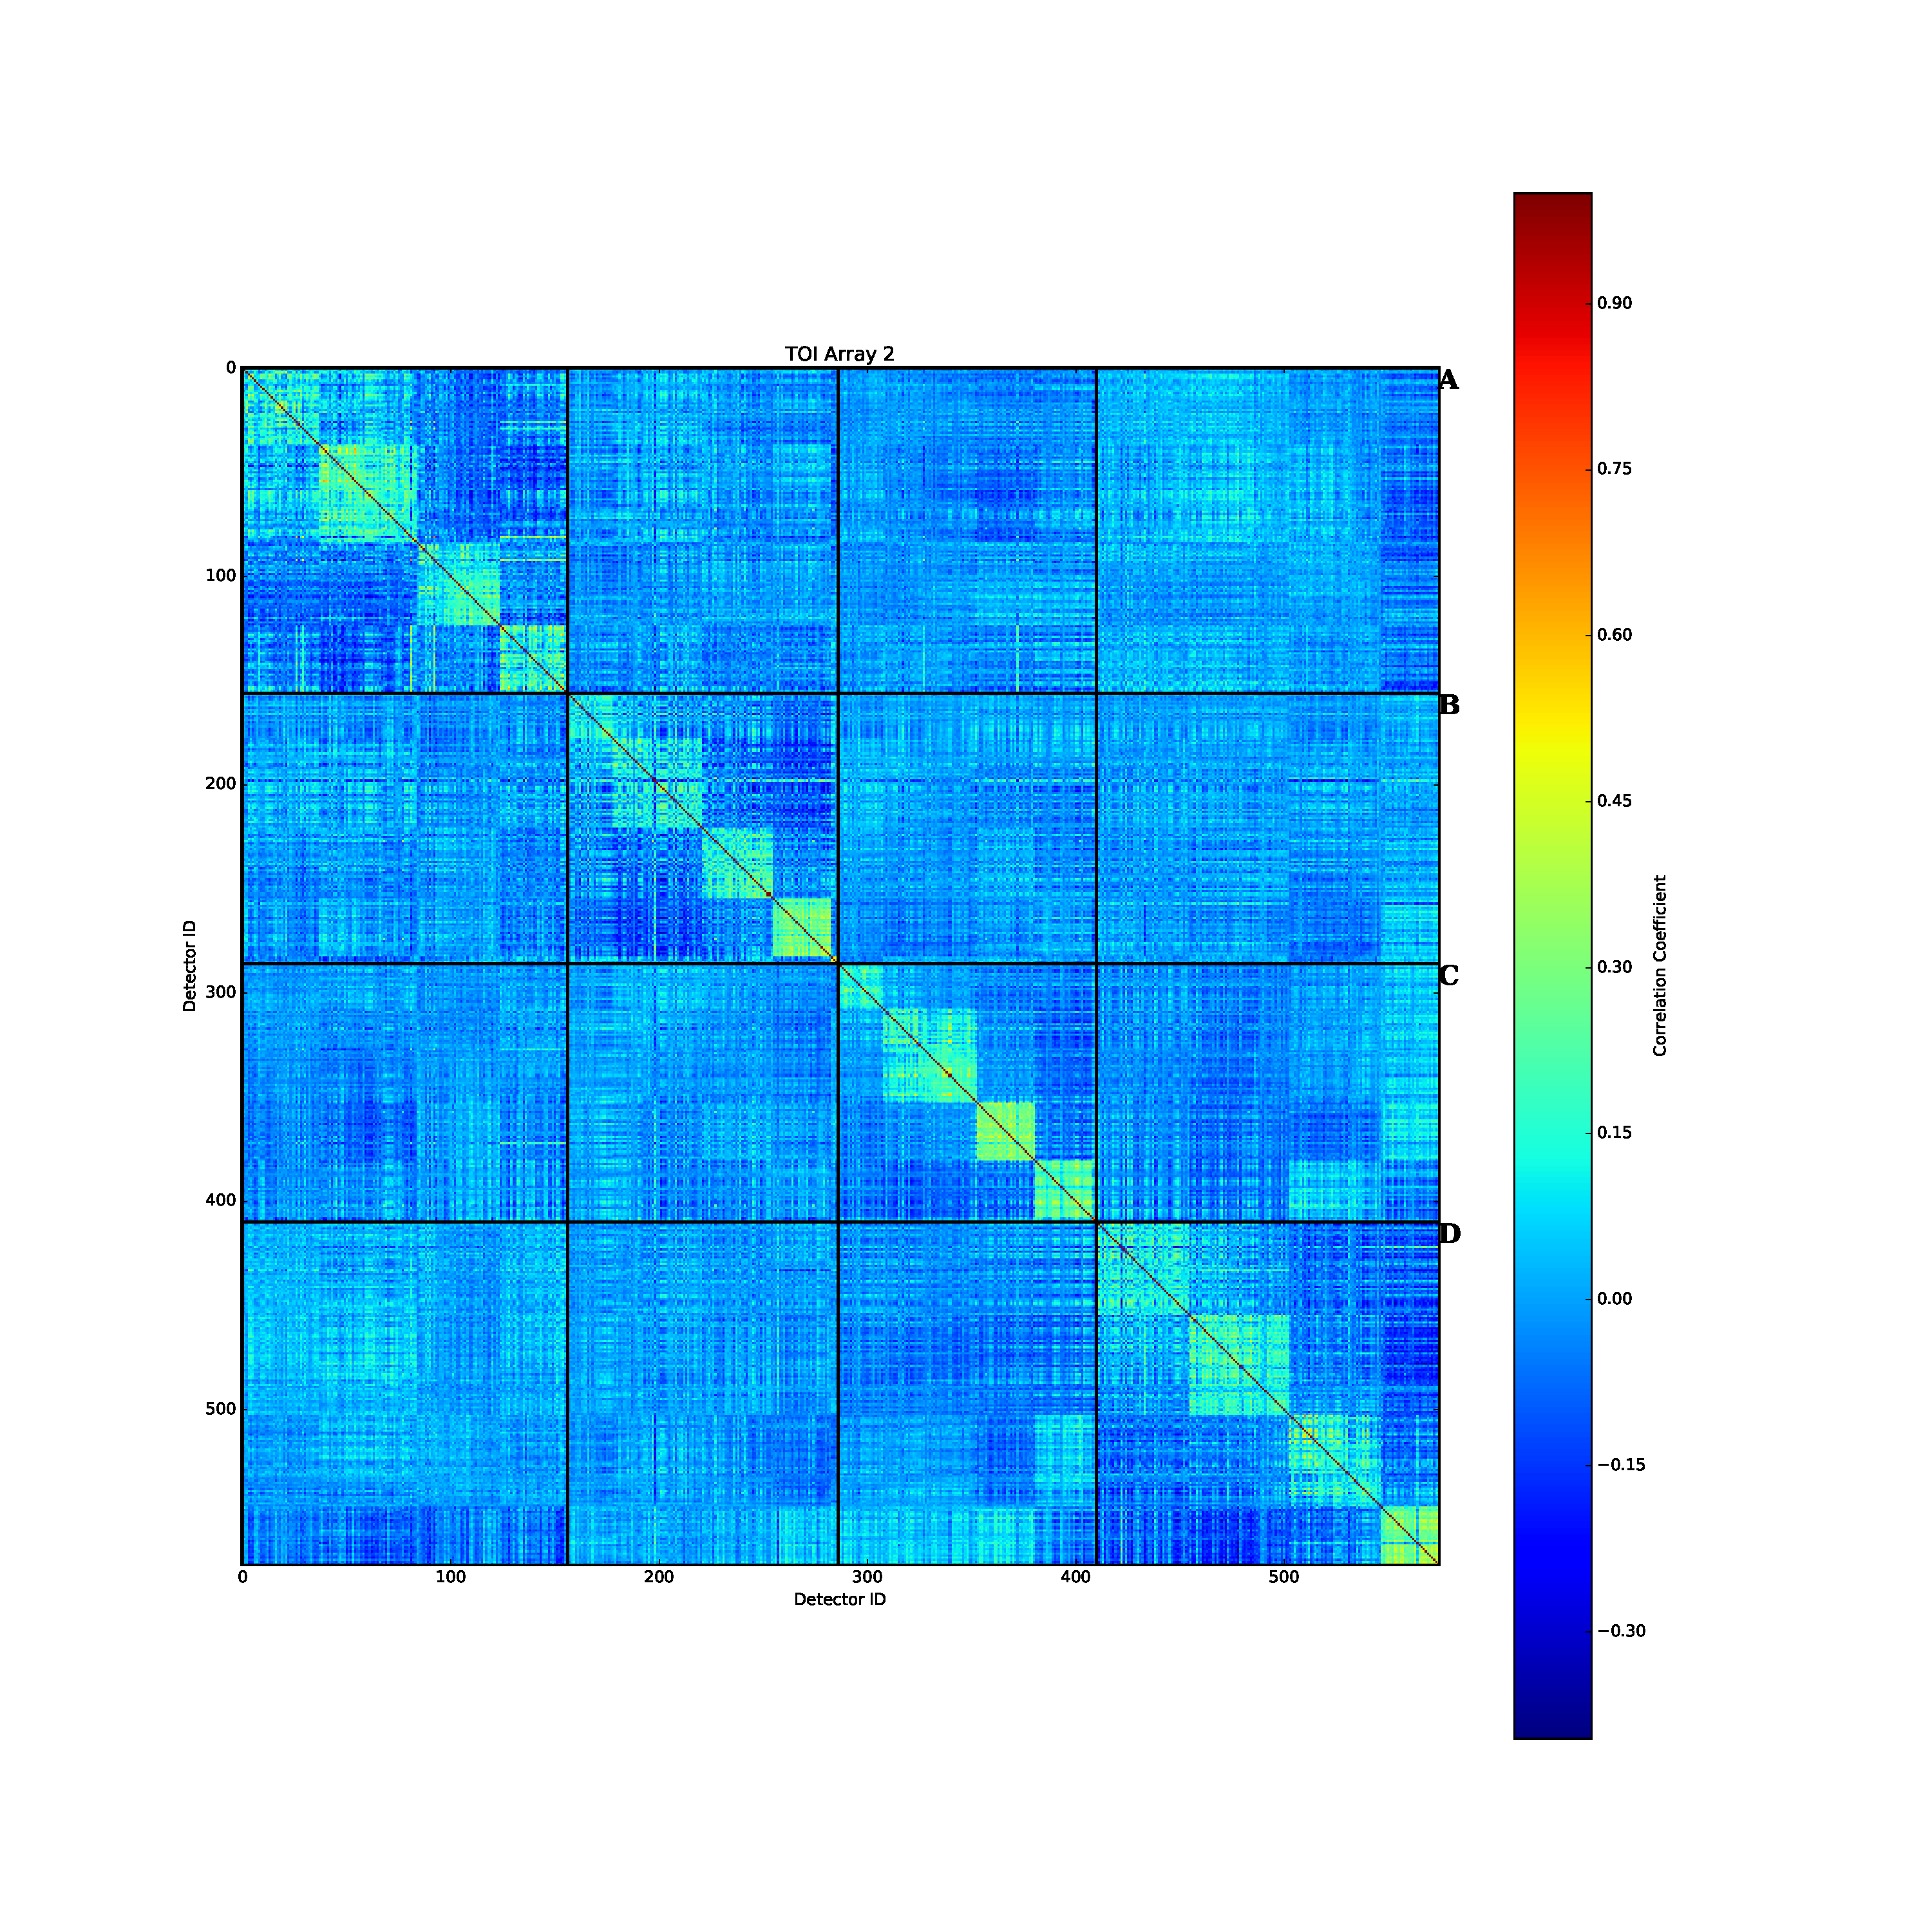
\includegraphics[width=0.3\textwidth]{Figures/DarkTests/corrmat_TOI_PCA_array_2_20161213s72.pdf}
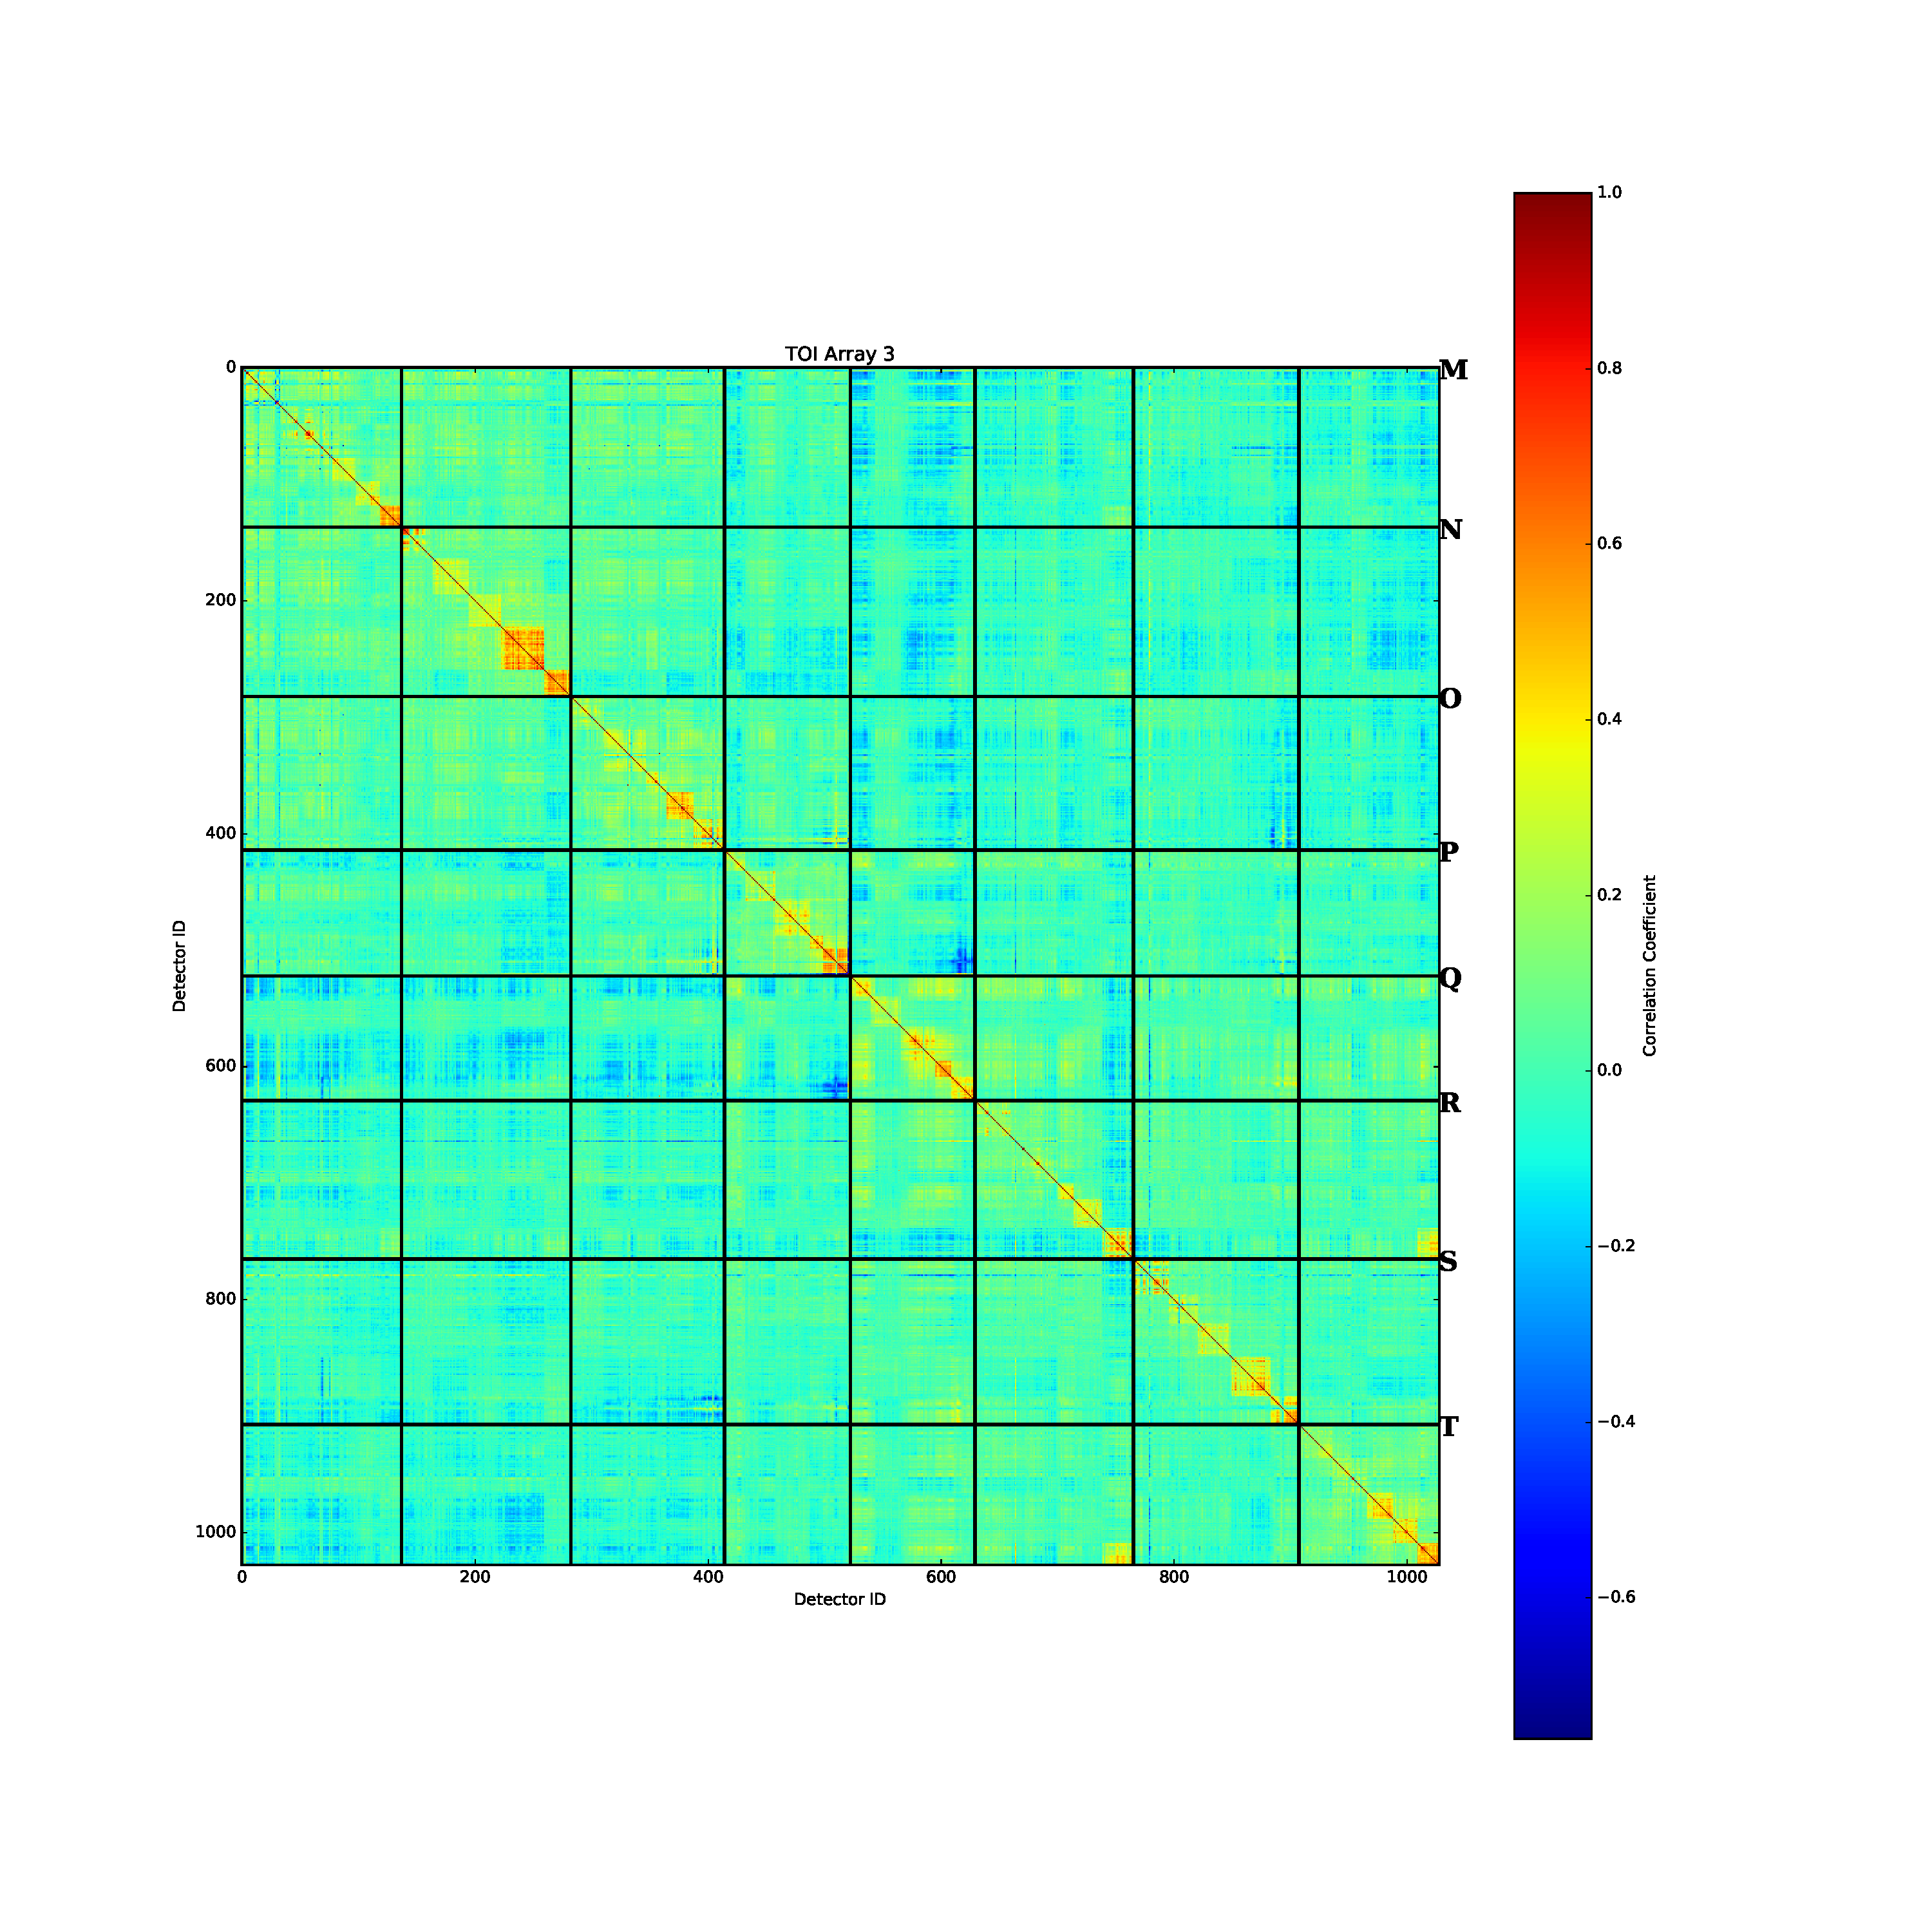
\includegraphics[width=0.3\textwidth]{Figures/DarkTests/corrmat_TOI_PCA_array_3_20161213s72.pdf}
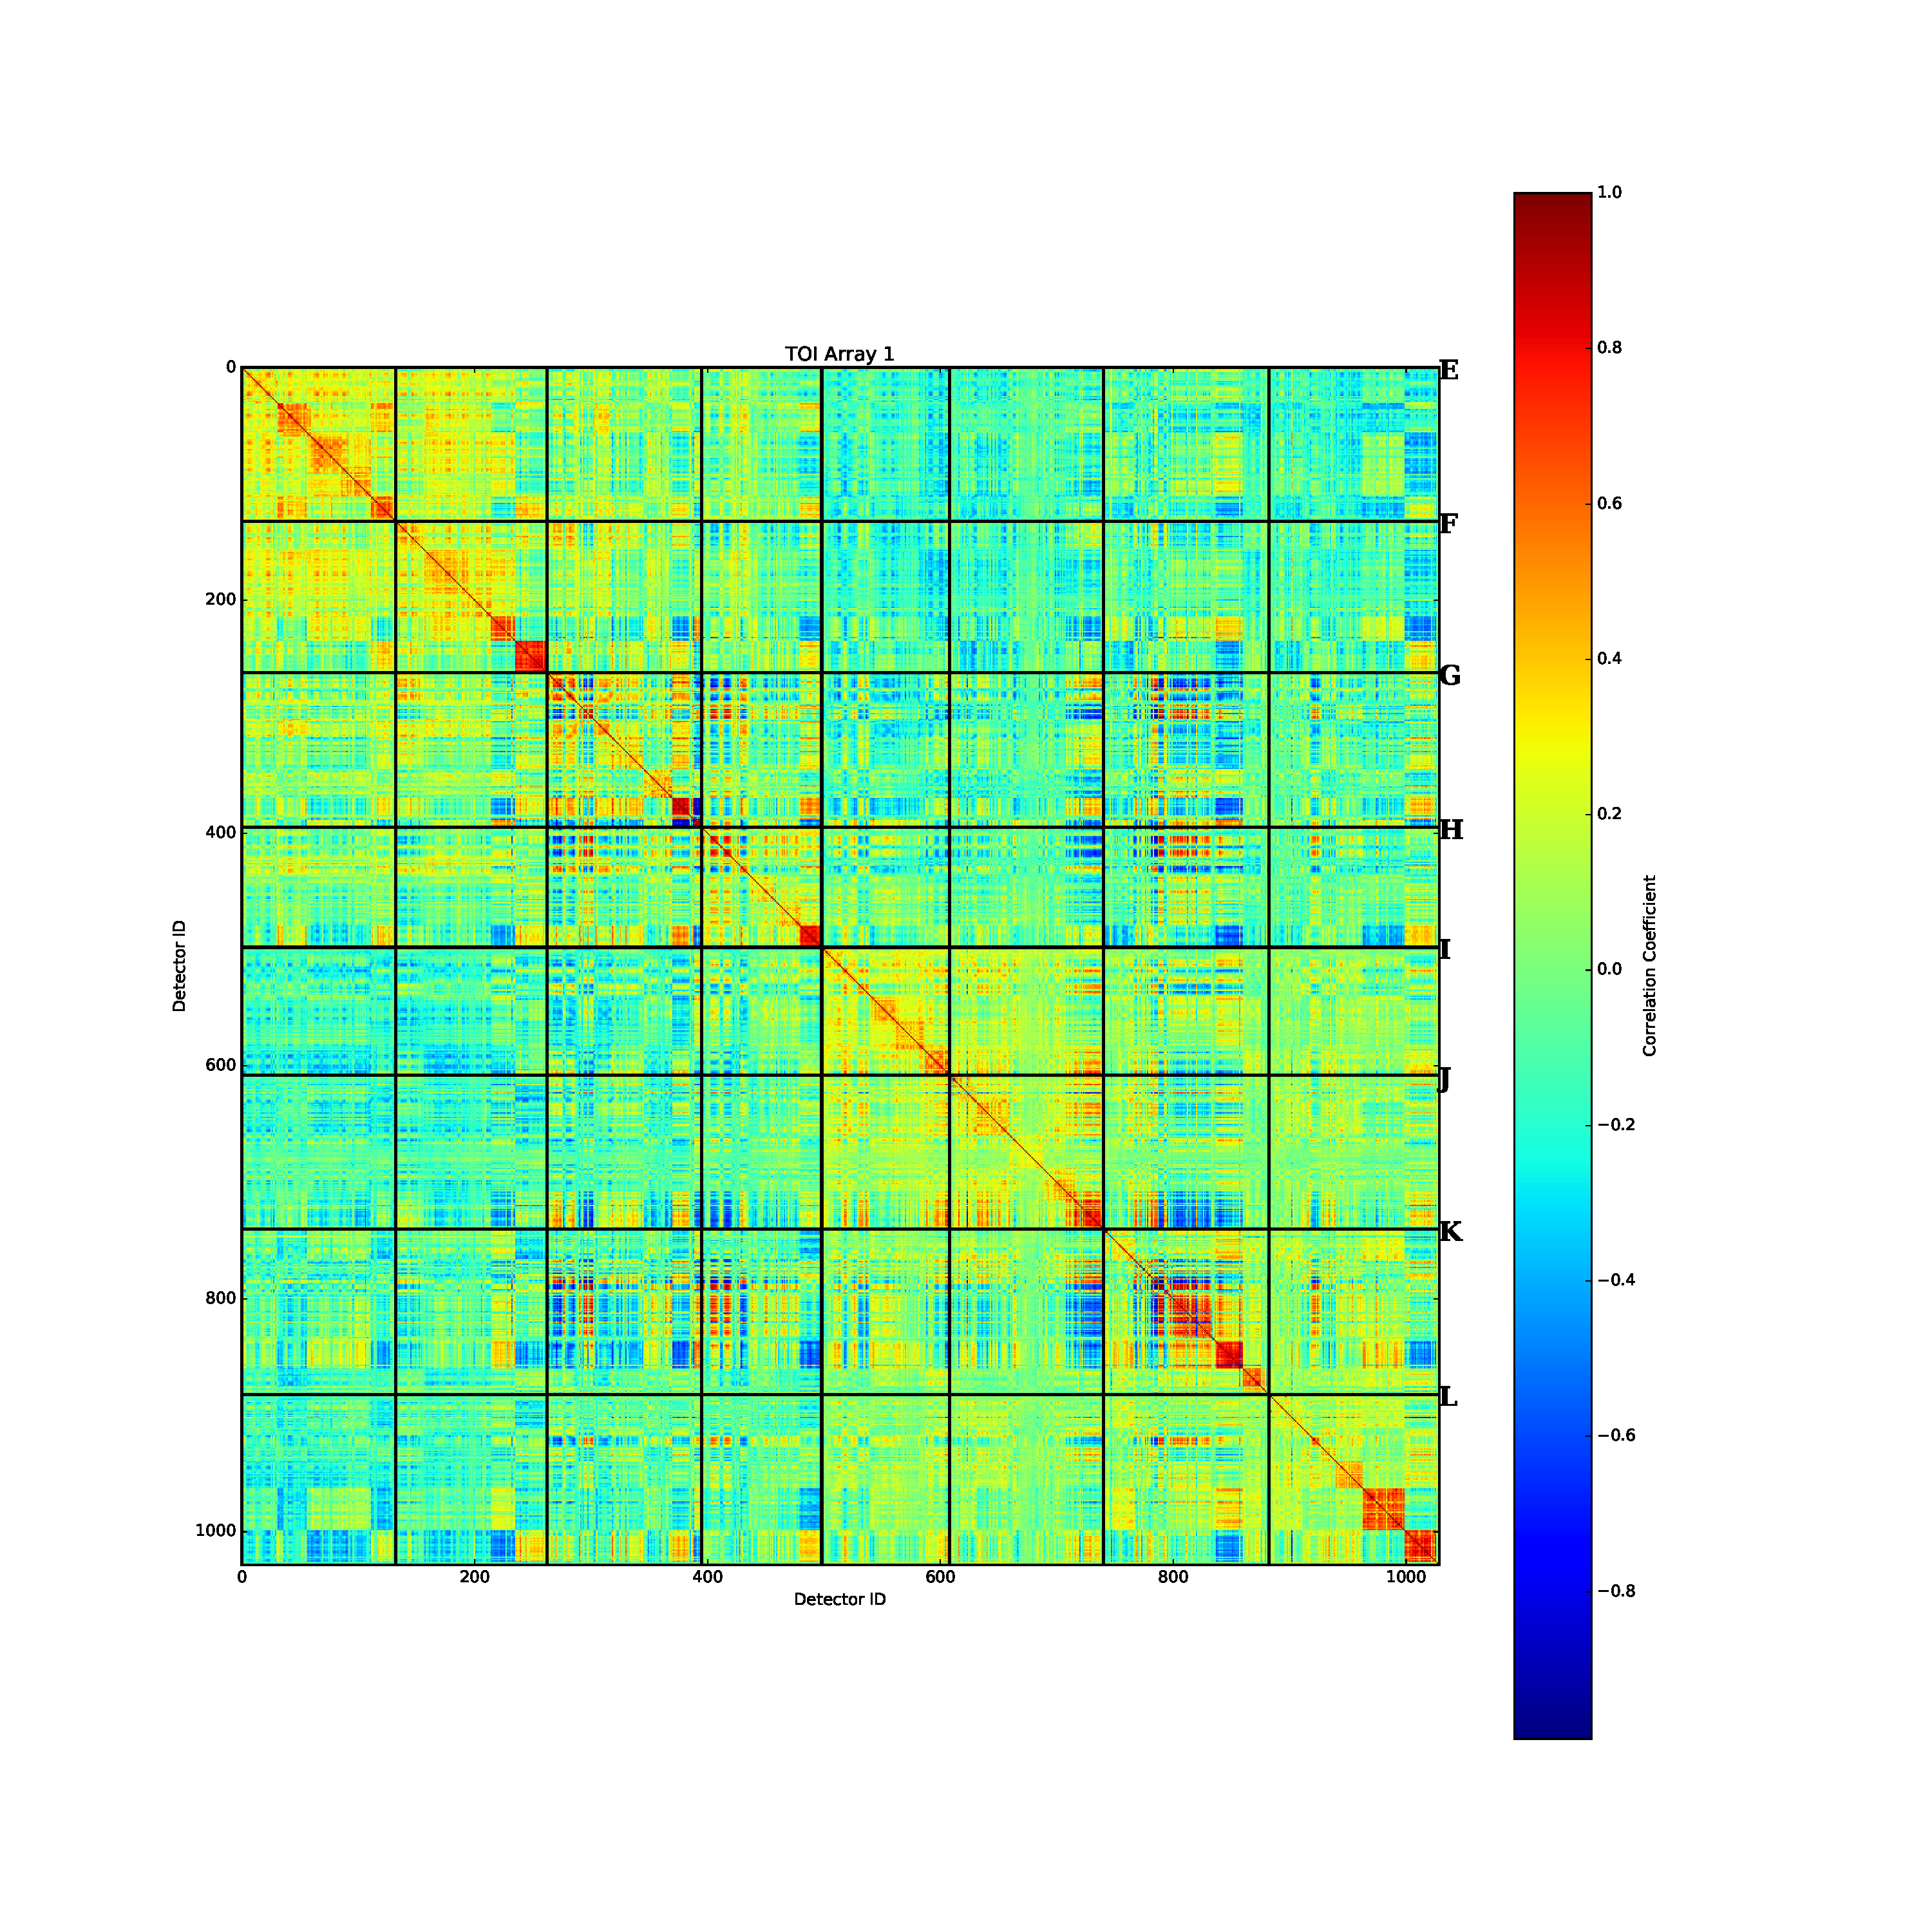
\includegraphics[width=0.3\textwidth]{Figures/DarkTests/corrmat_TOI_BC_array_1_20161213s72.pdf}
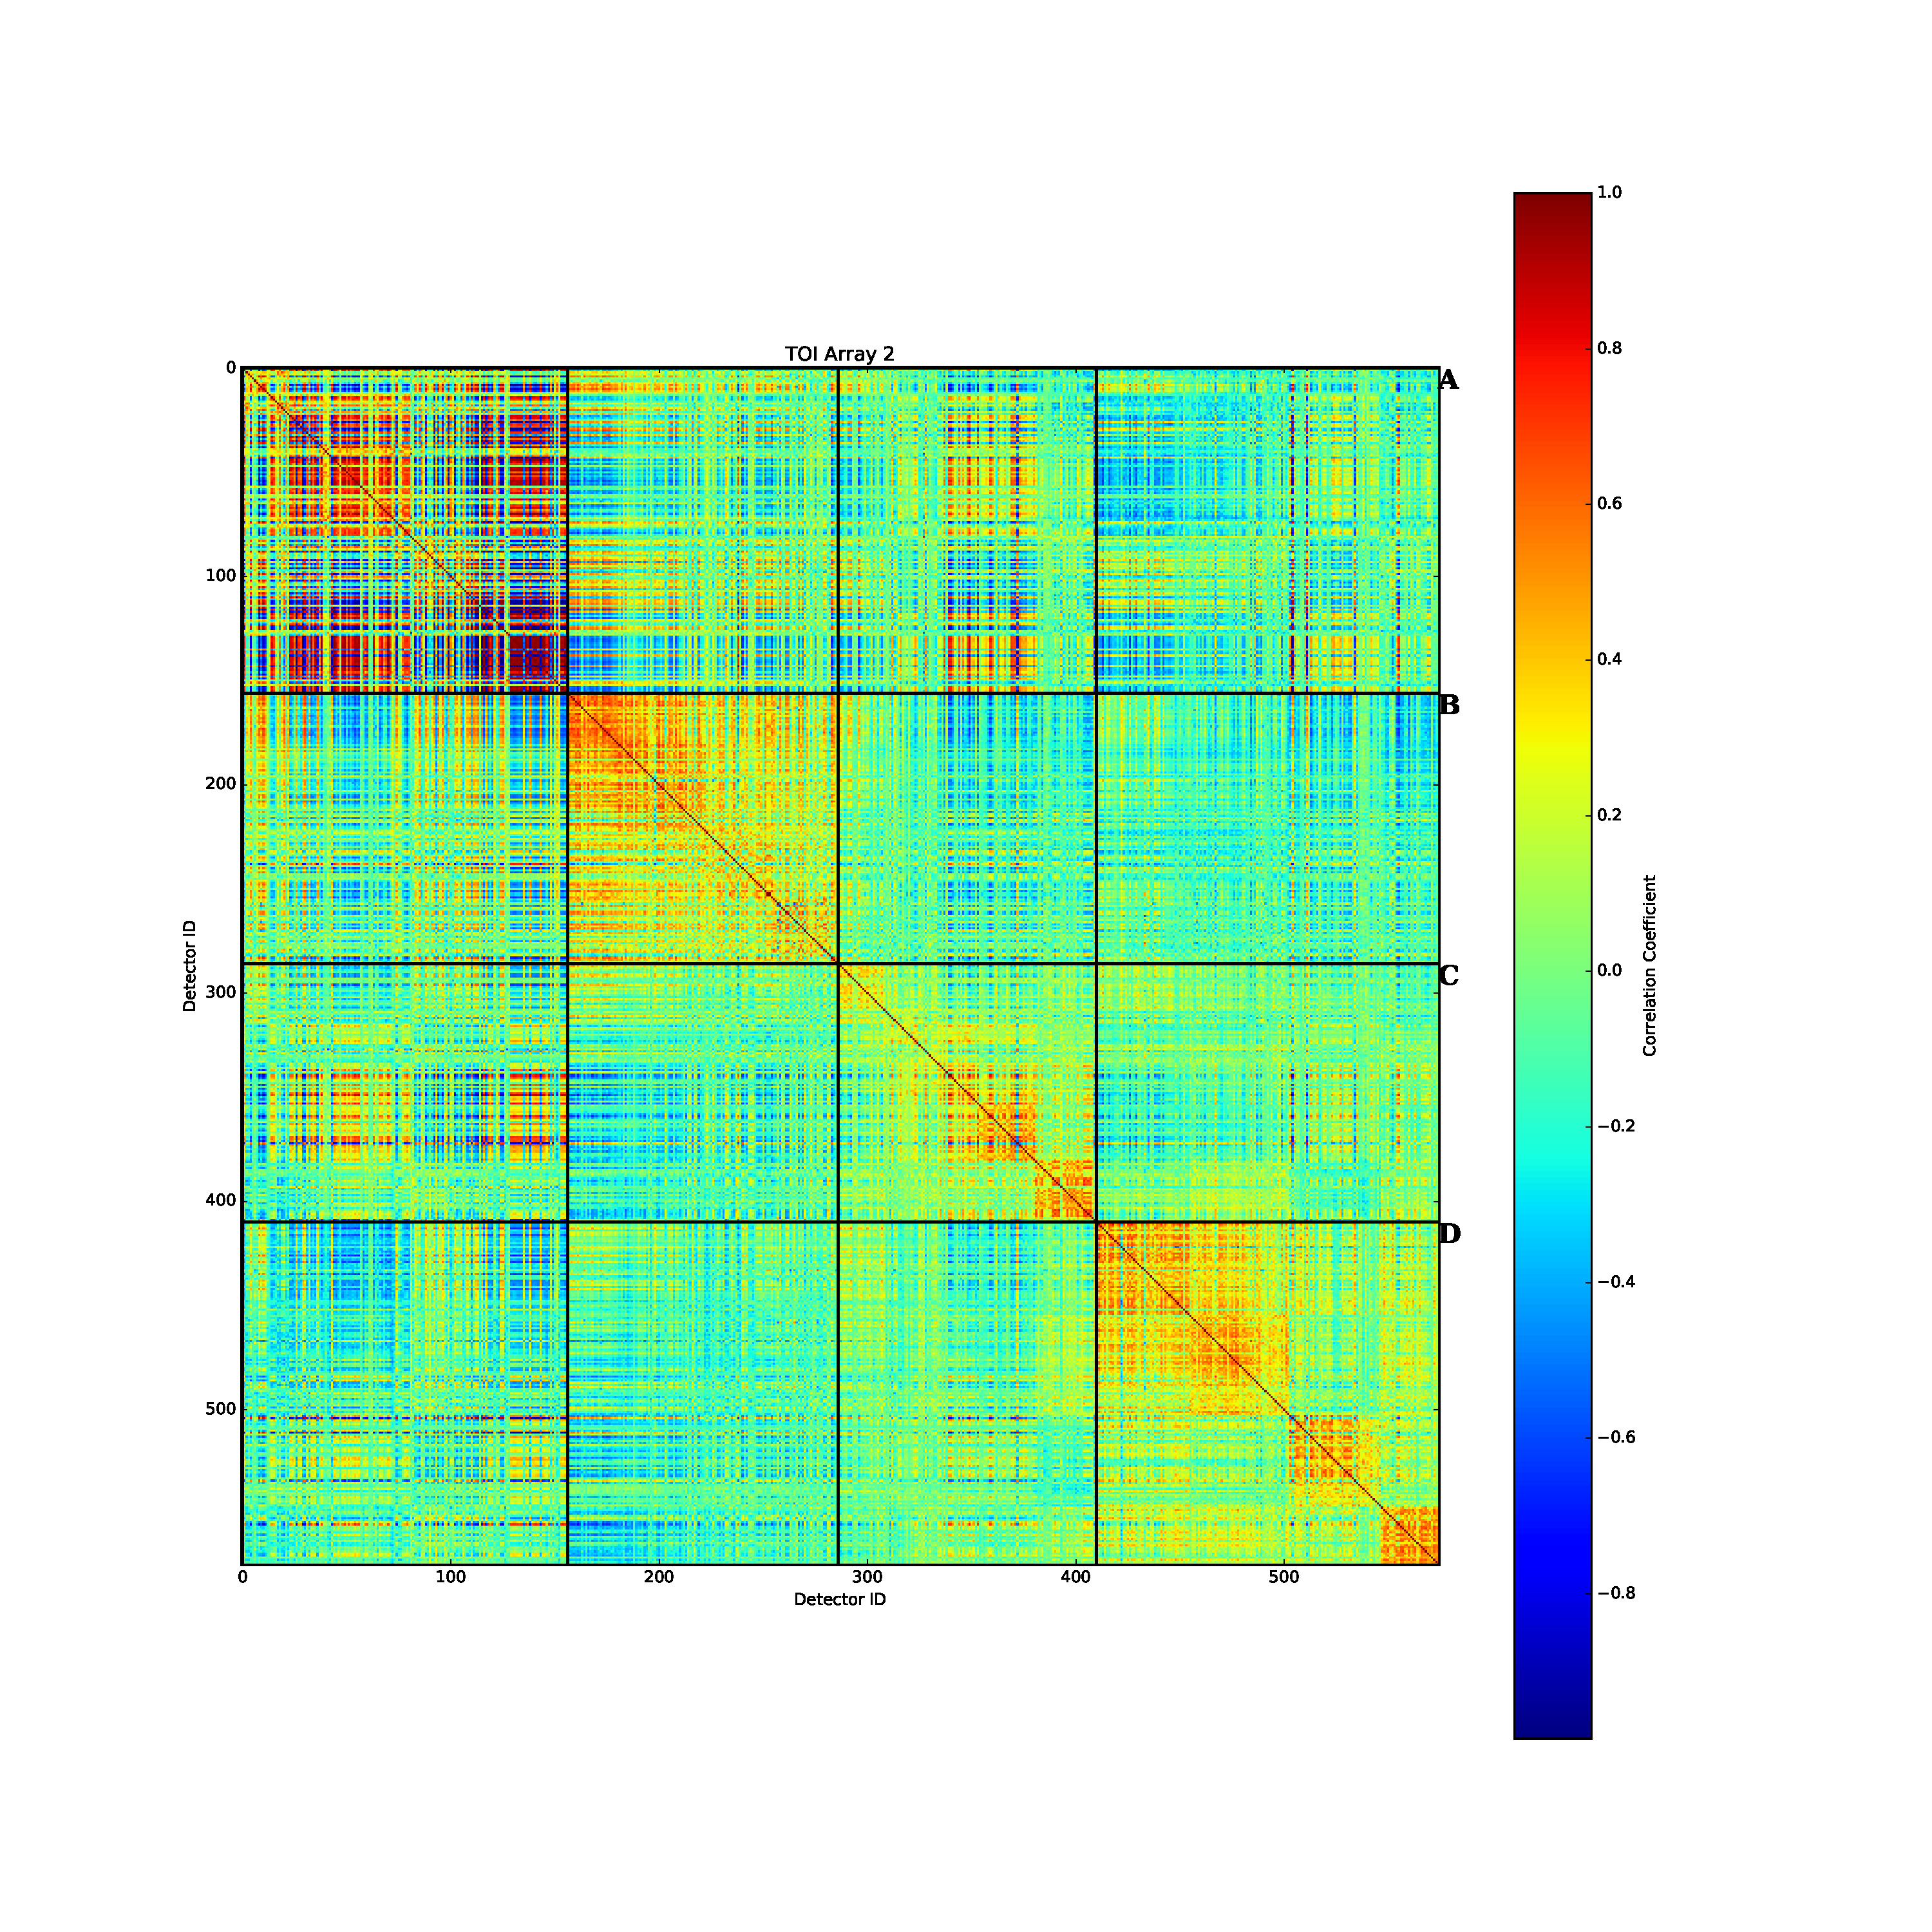
\includegraphics[width=0.3\textwidth]{Figures/DarkTests/corrmat_TOI_BC_array_2_20161213s72.pdf}
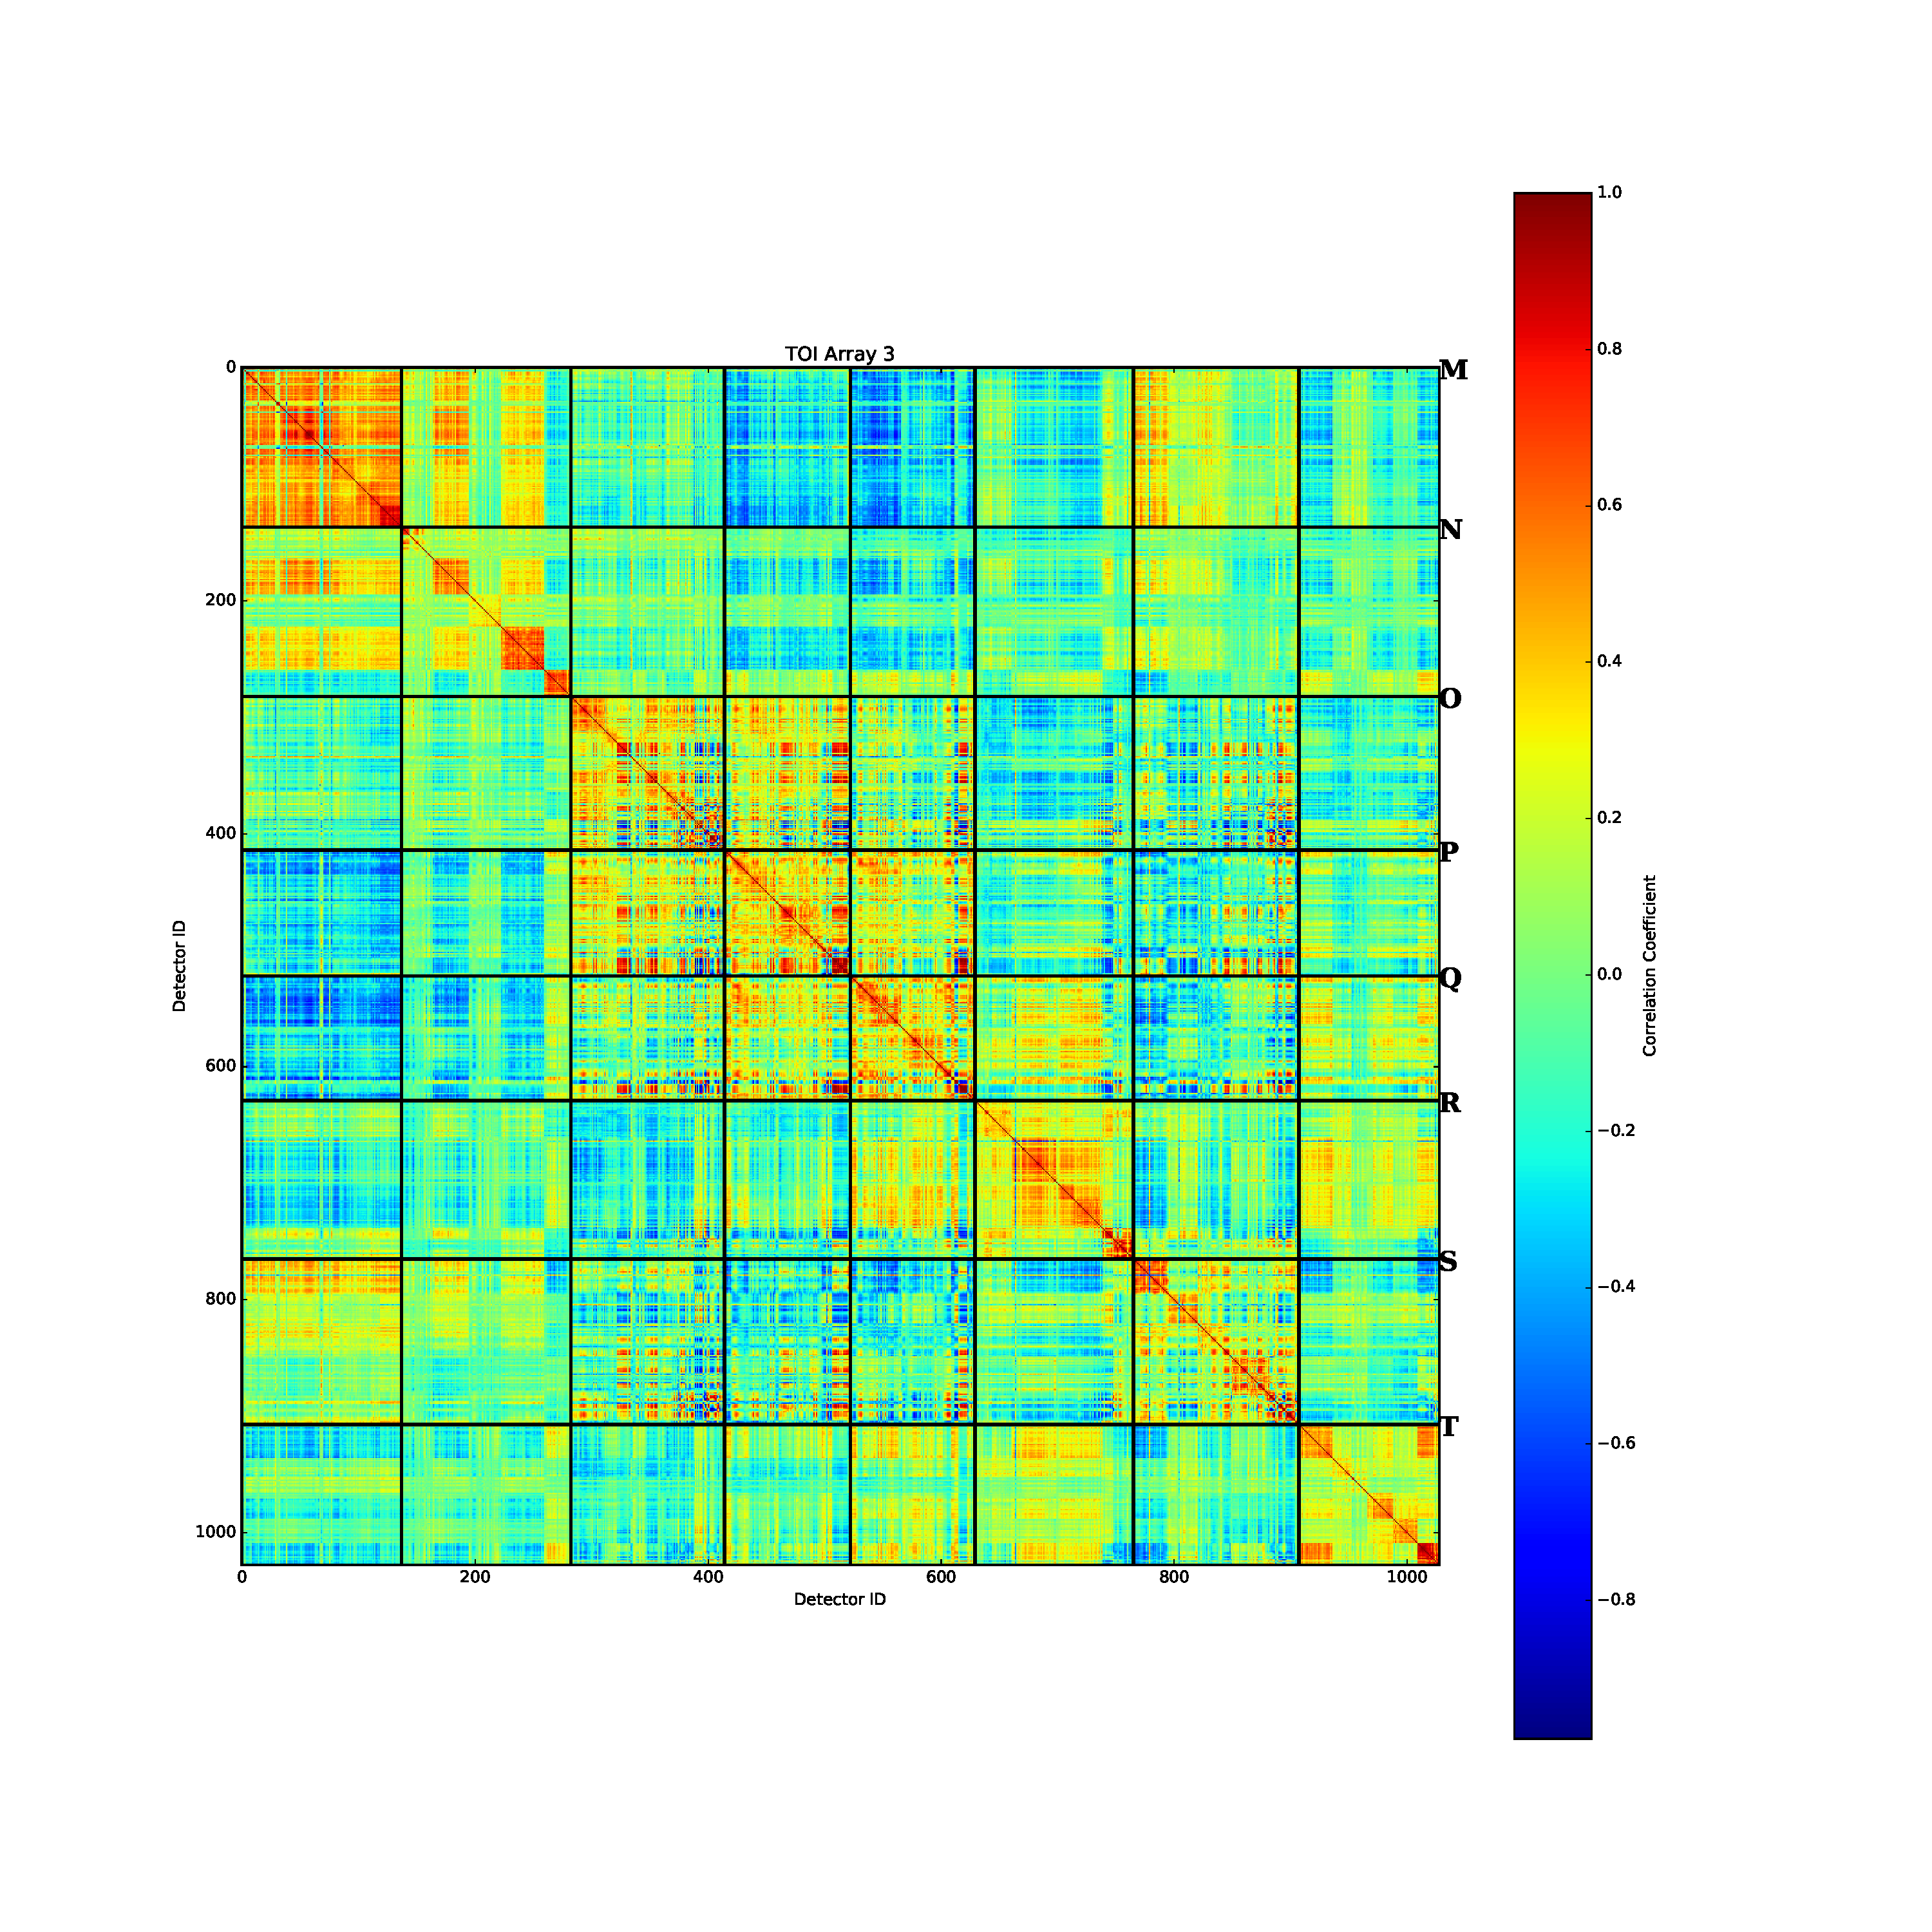
\includegraphics[width=0.3\textwidth]{Figures/DarkTests/corrmat_TOI_BC_array_3_20161213s72.pdf}
\end{center}
\caption{From left to right correlation matrices for the three NIKA2 arrays (A1, A2, and A3) for scan 20161213s72. From top to bottom we present the correlation of the raw data, after CM, PCA and BC decorrelations. \label{corrs72}}
\end{figure}


\begin{figure}[ht] % Inline image example
\begin{center}
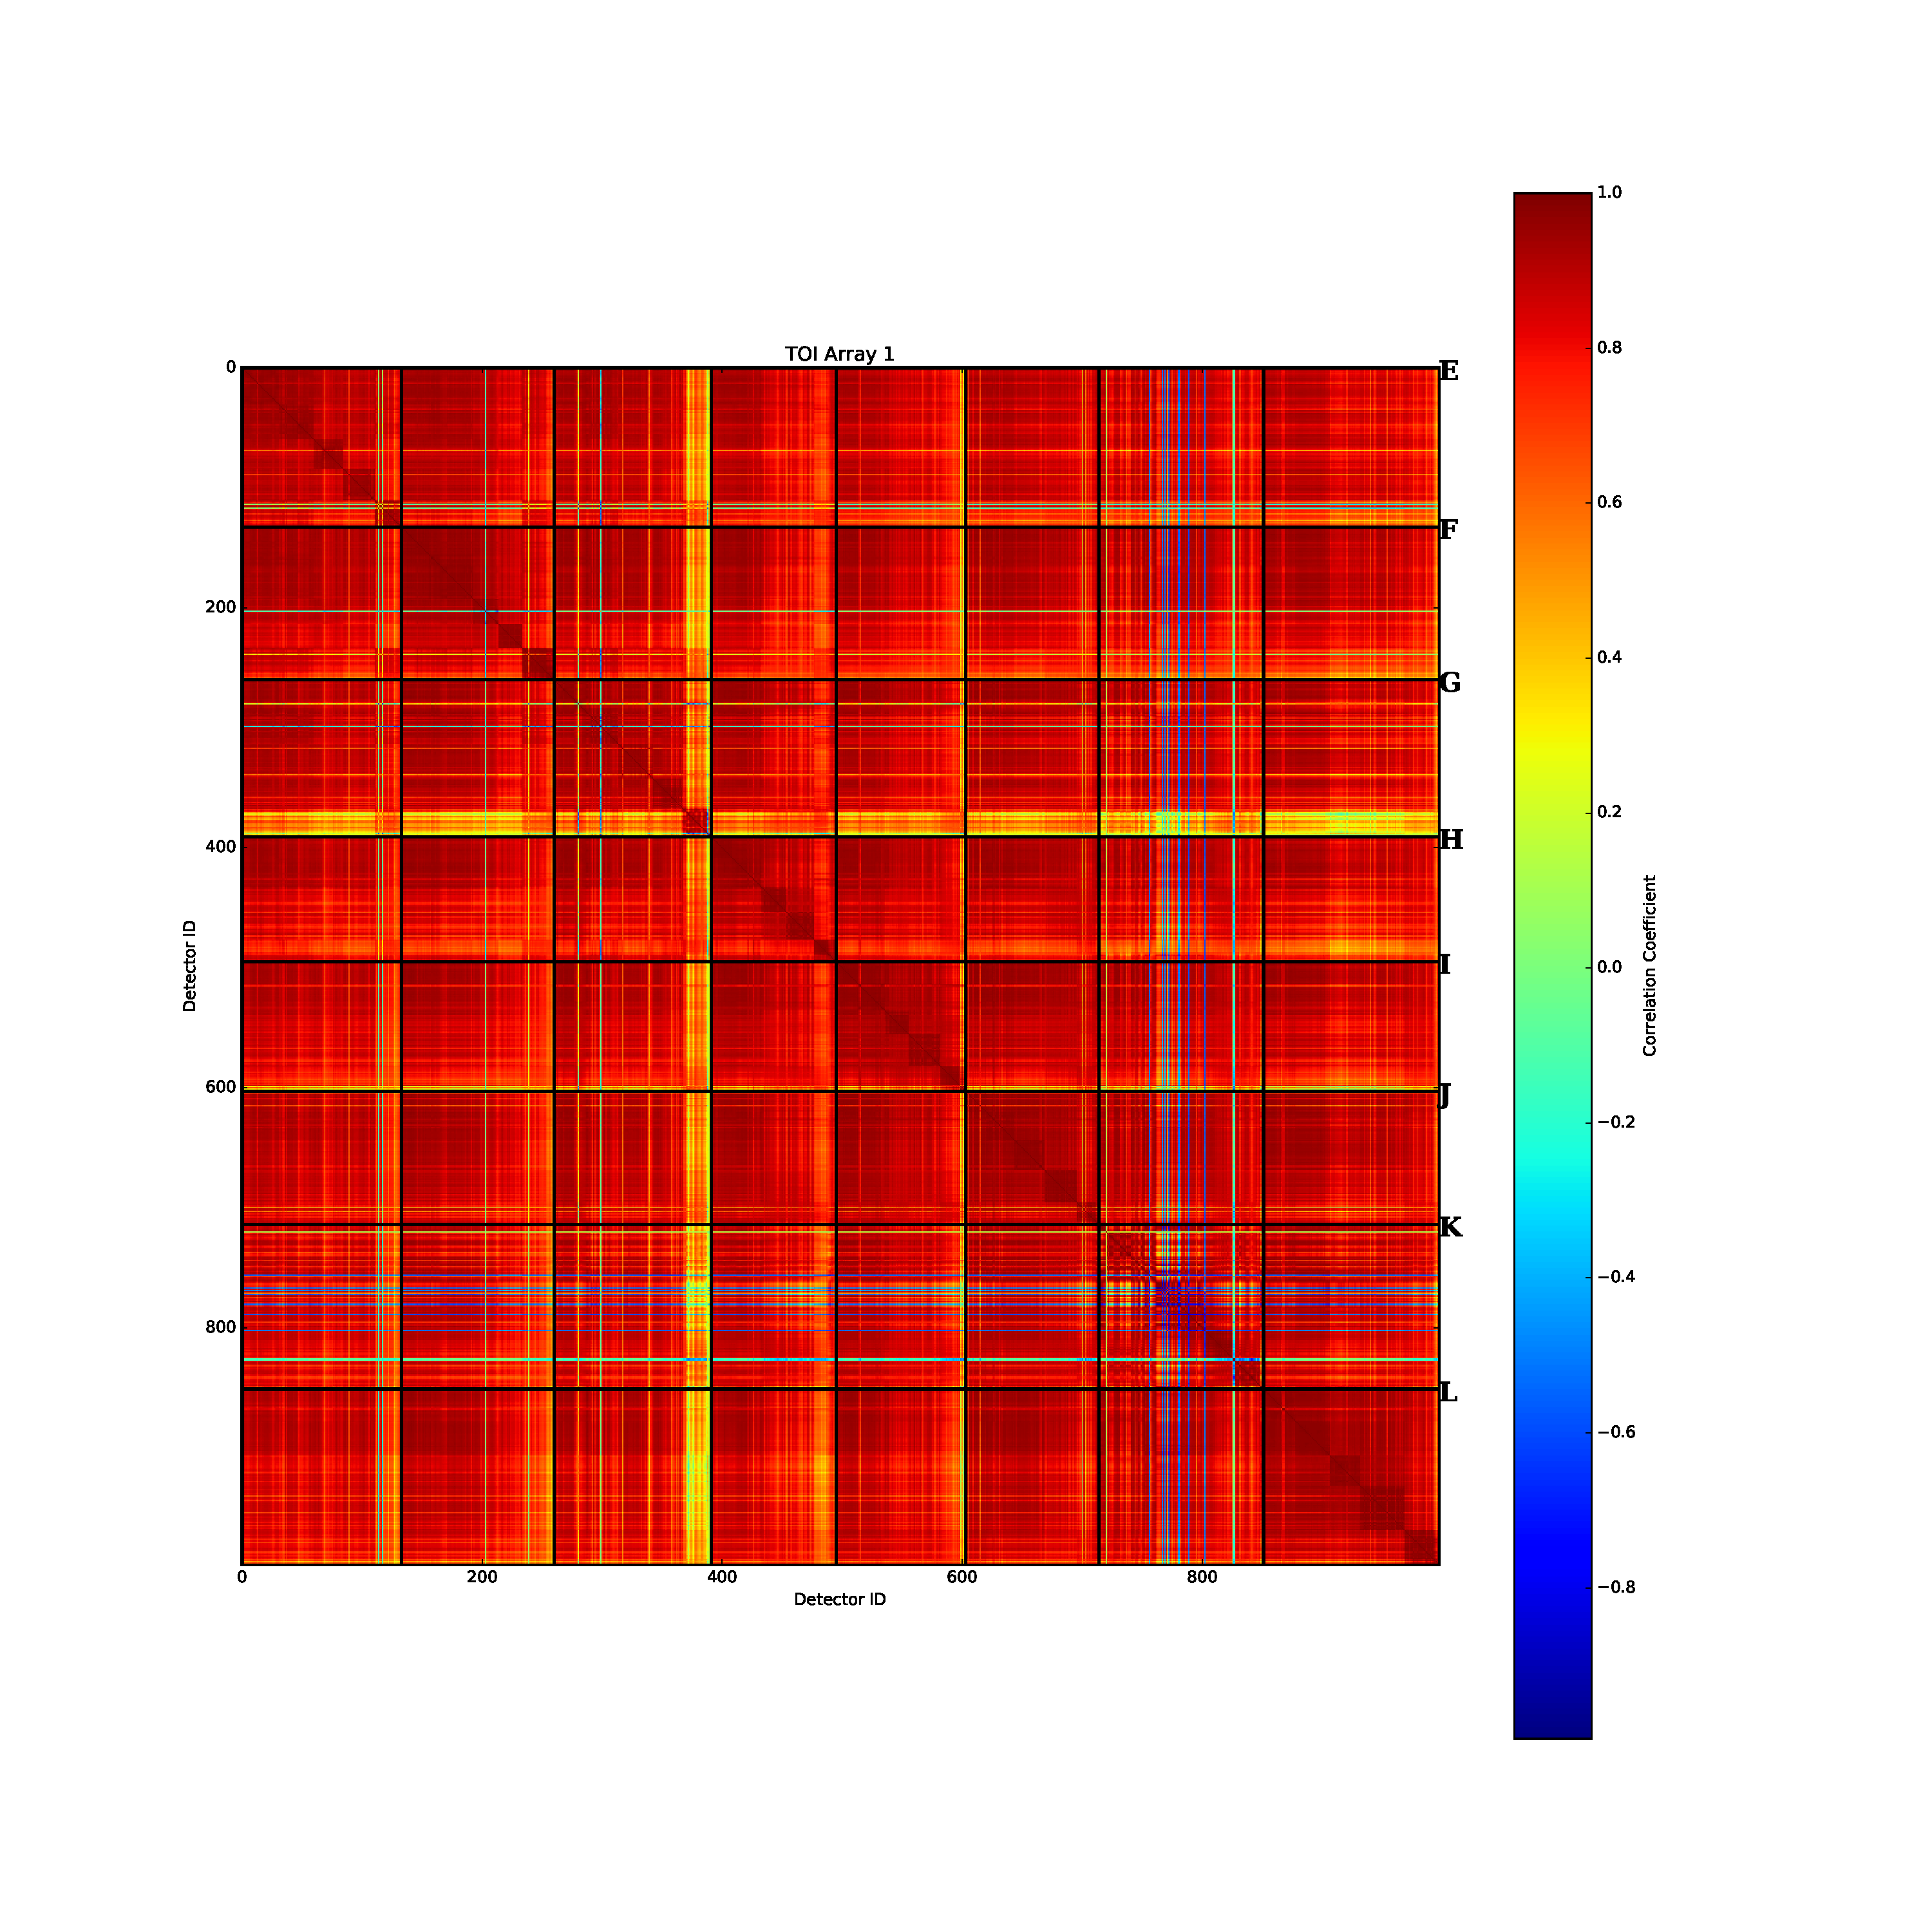
\includegraphics[width=0.3\textwidth]{Figures/DarkTests/corrmat_TOI_array_1_20160504s97.pdf}
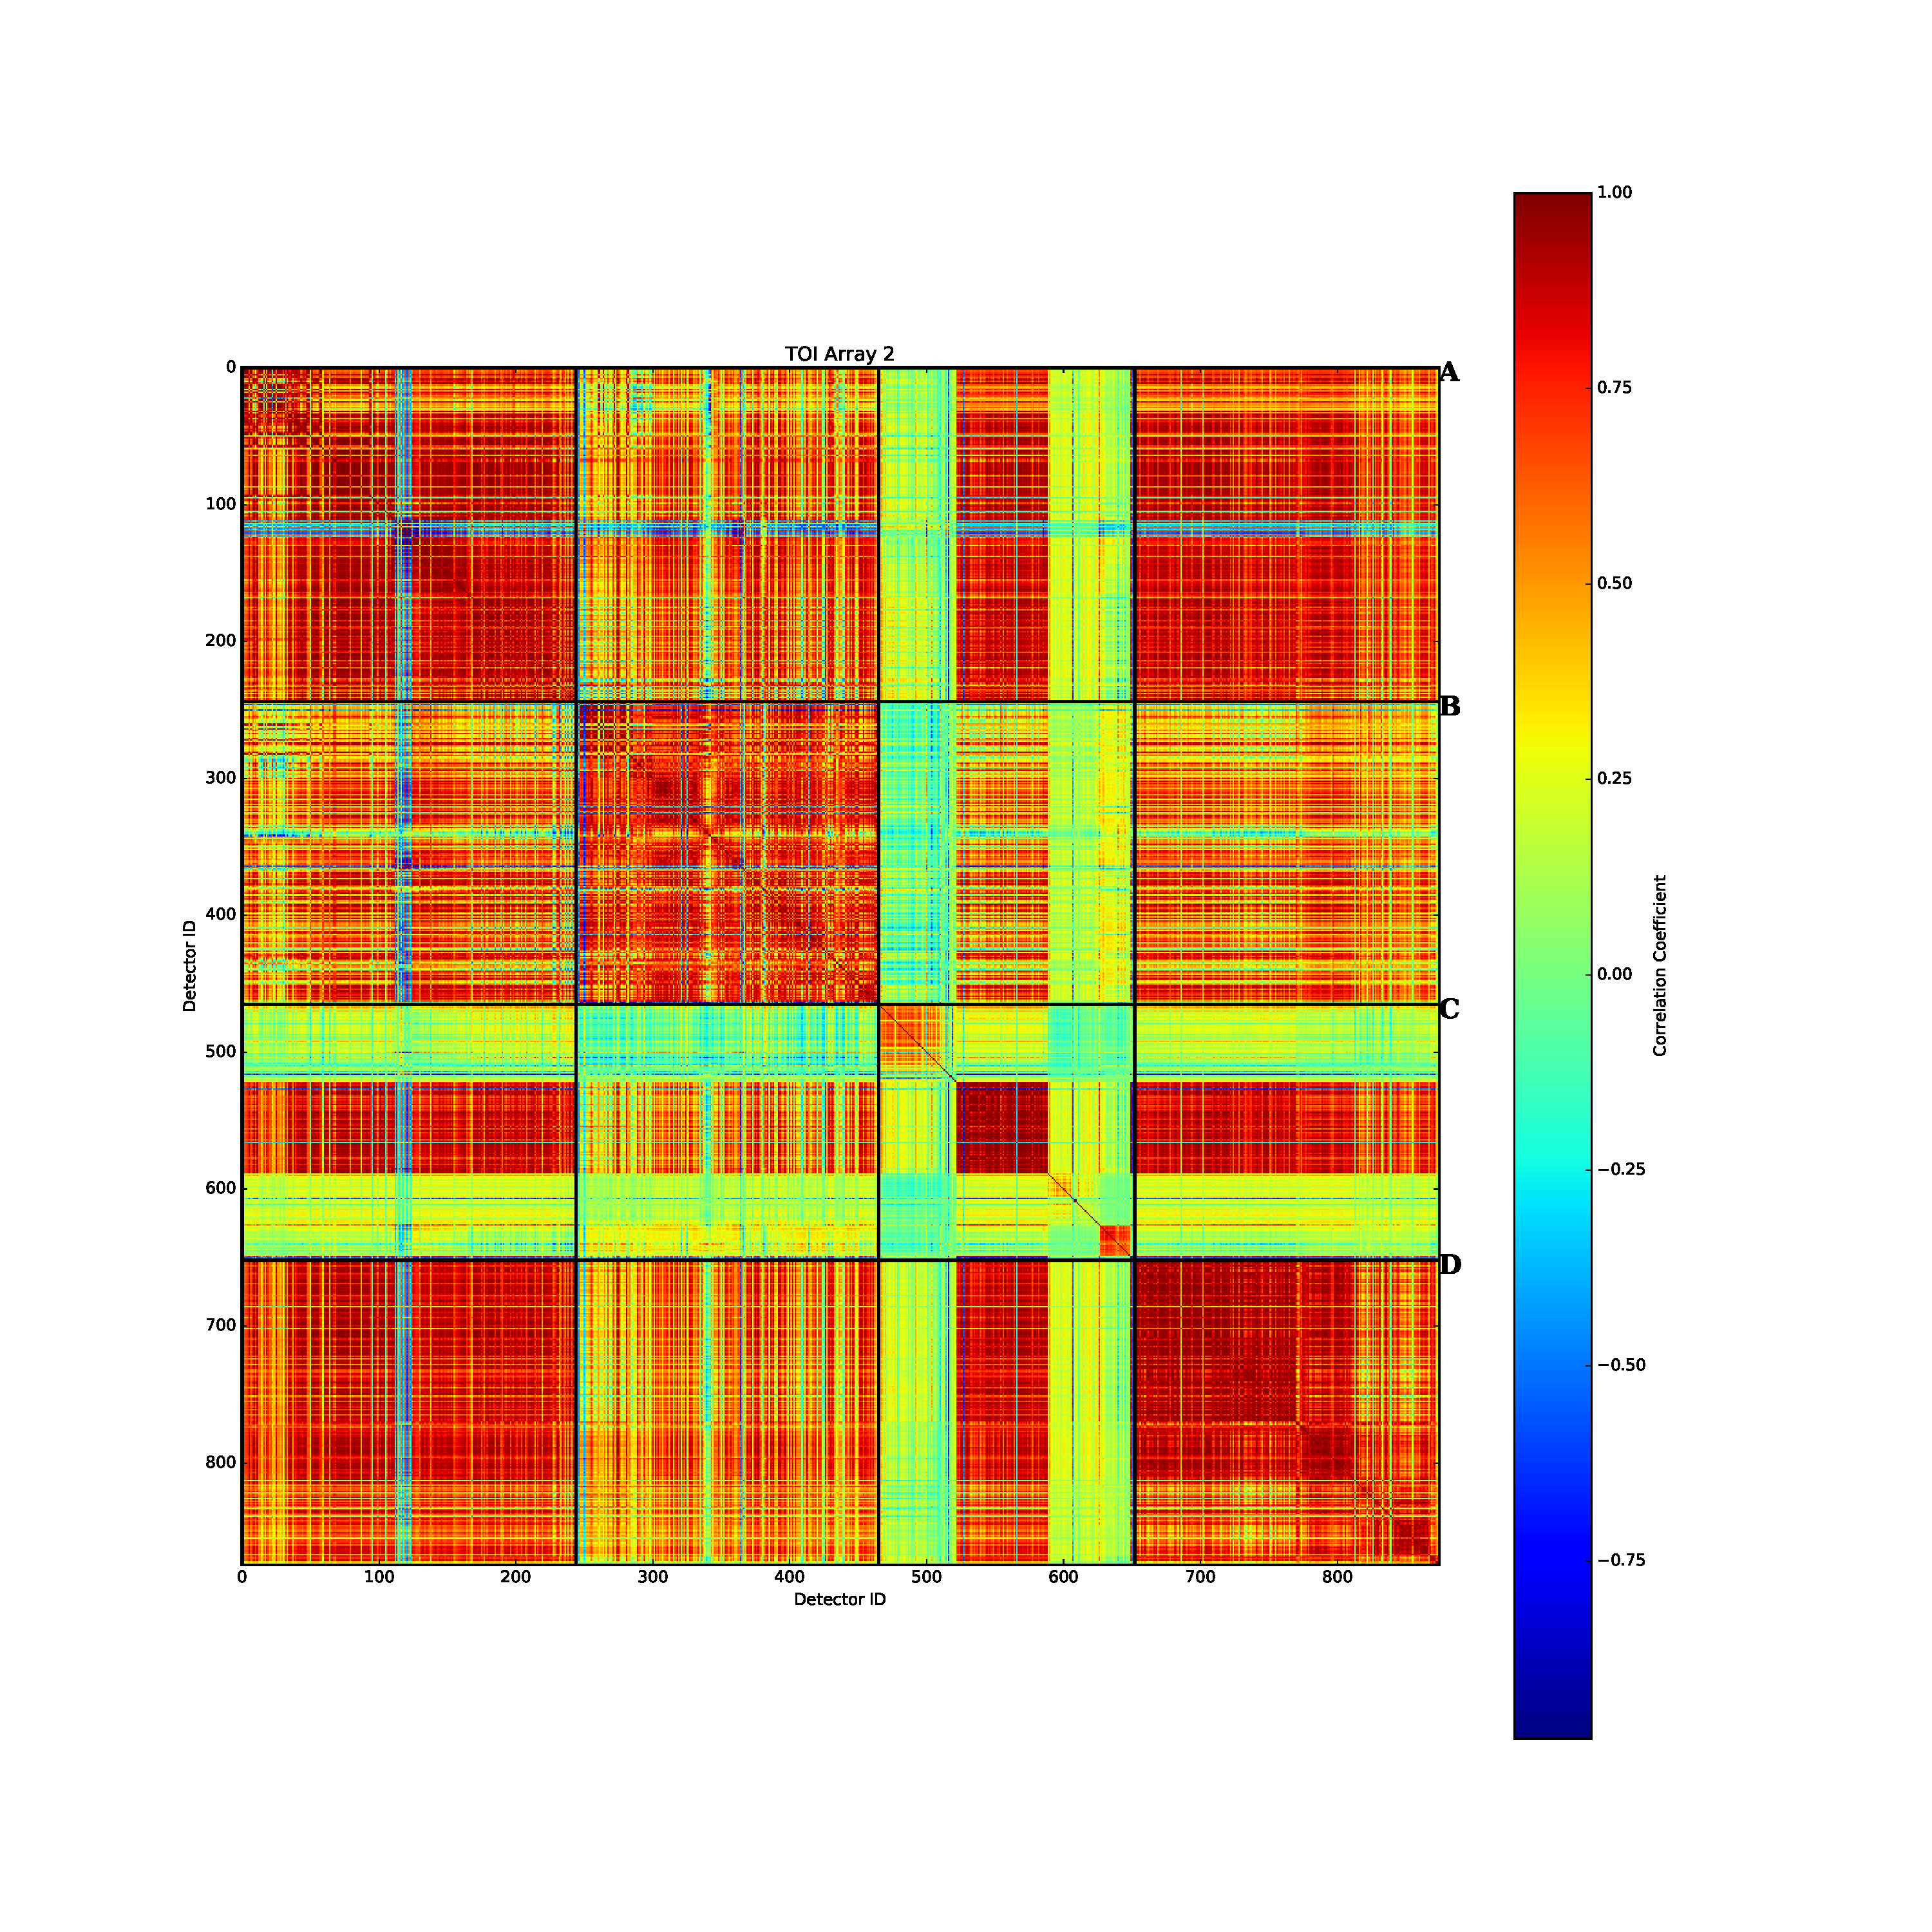
\includegraphics[width=0.3\textwidth]{Figures/DarkTests/corrmat_TOI_array_2_20160504s97.pdf}
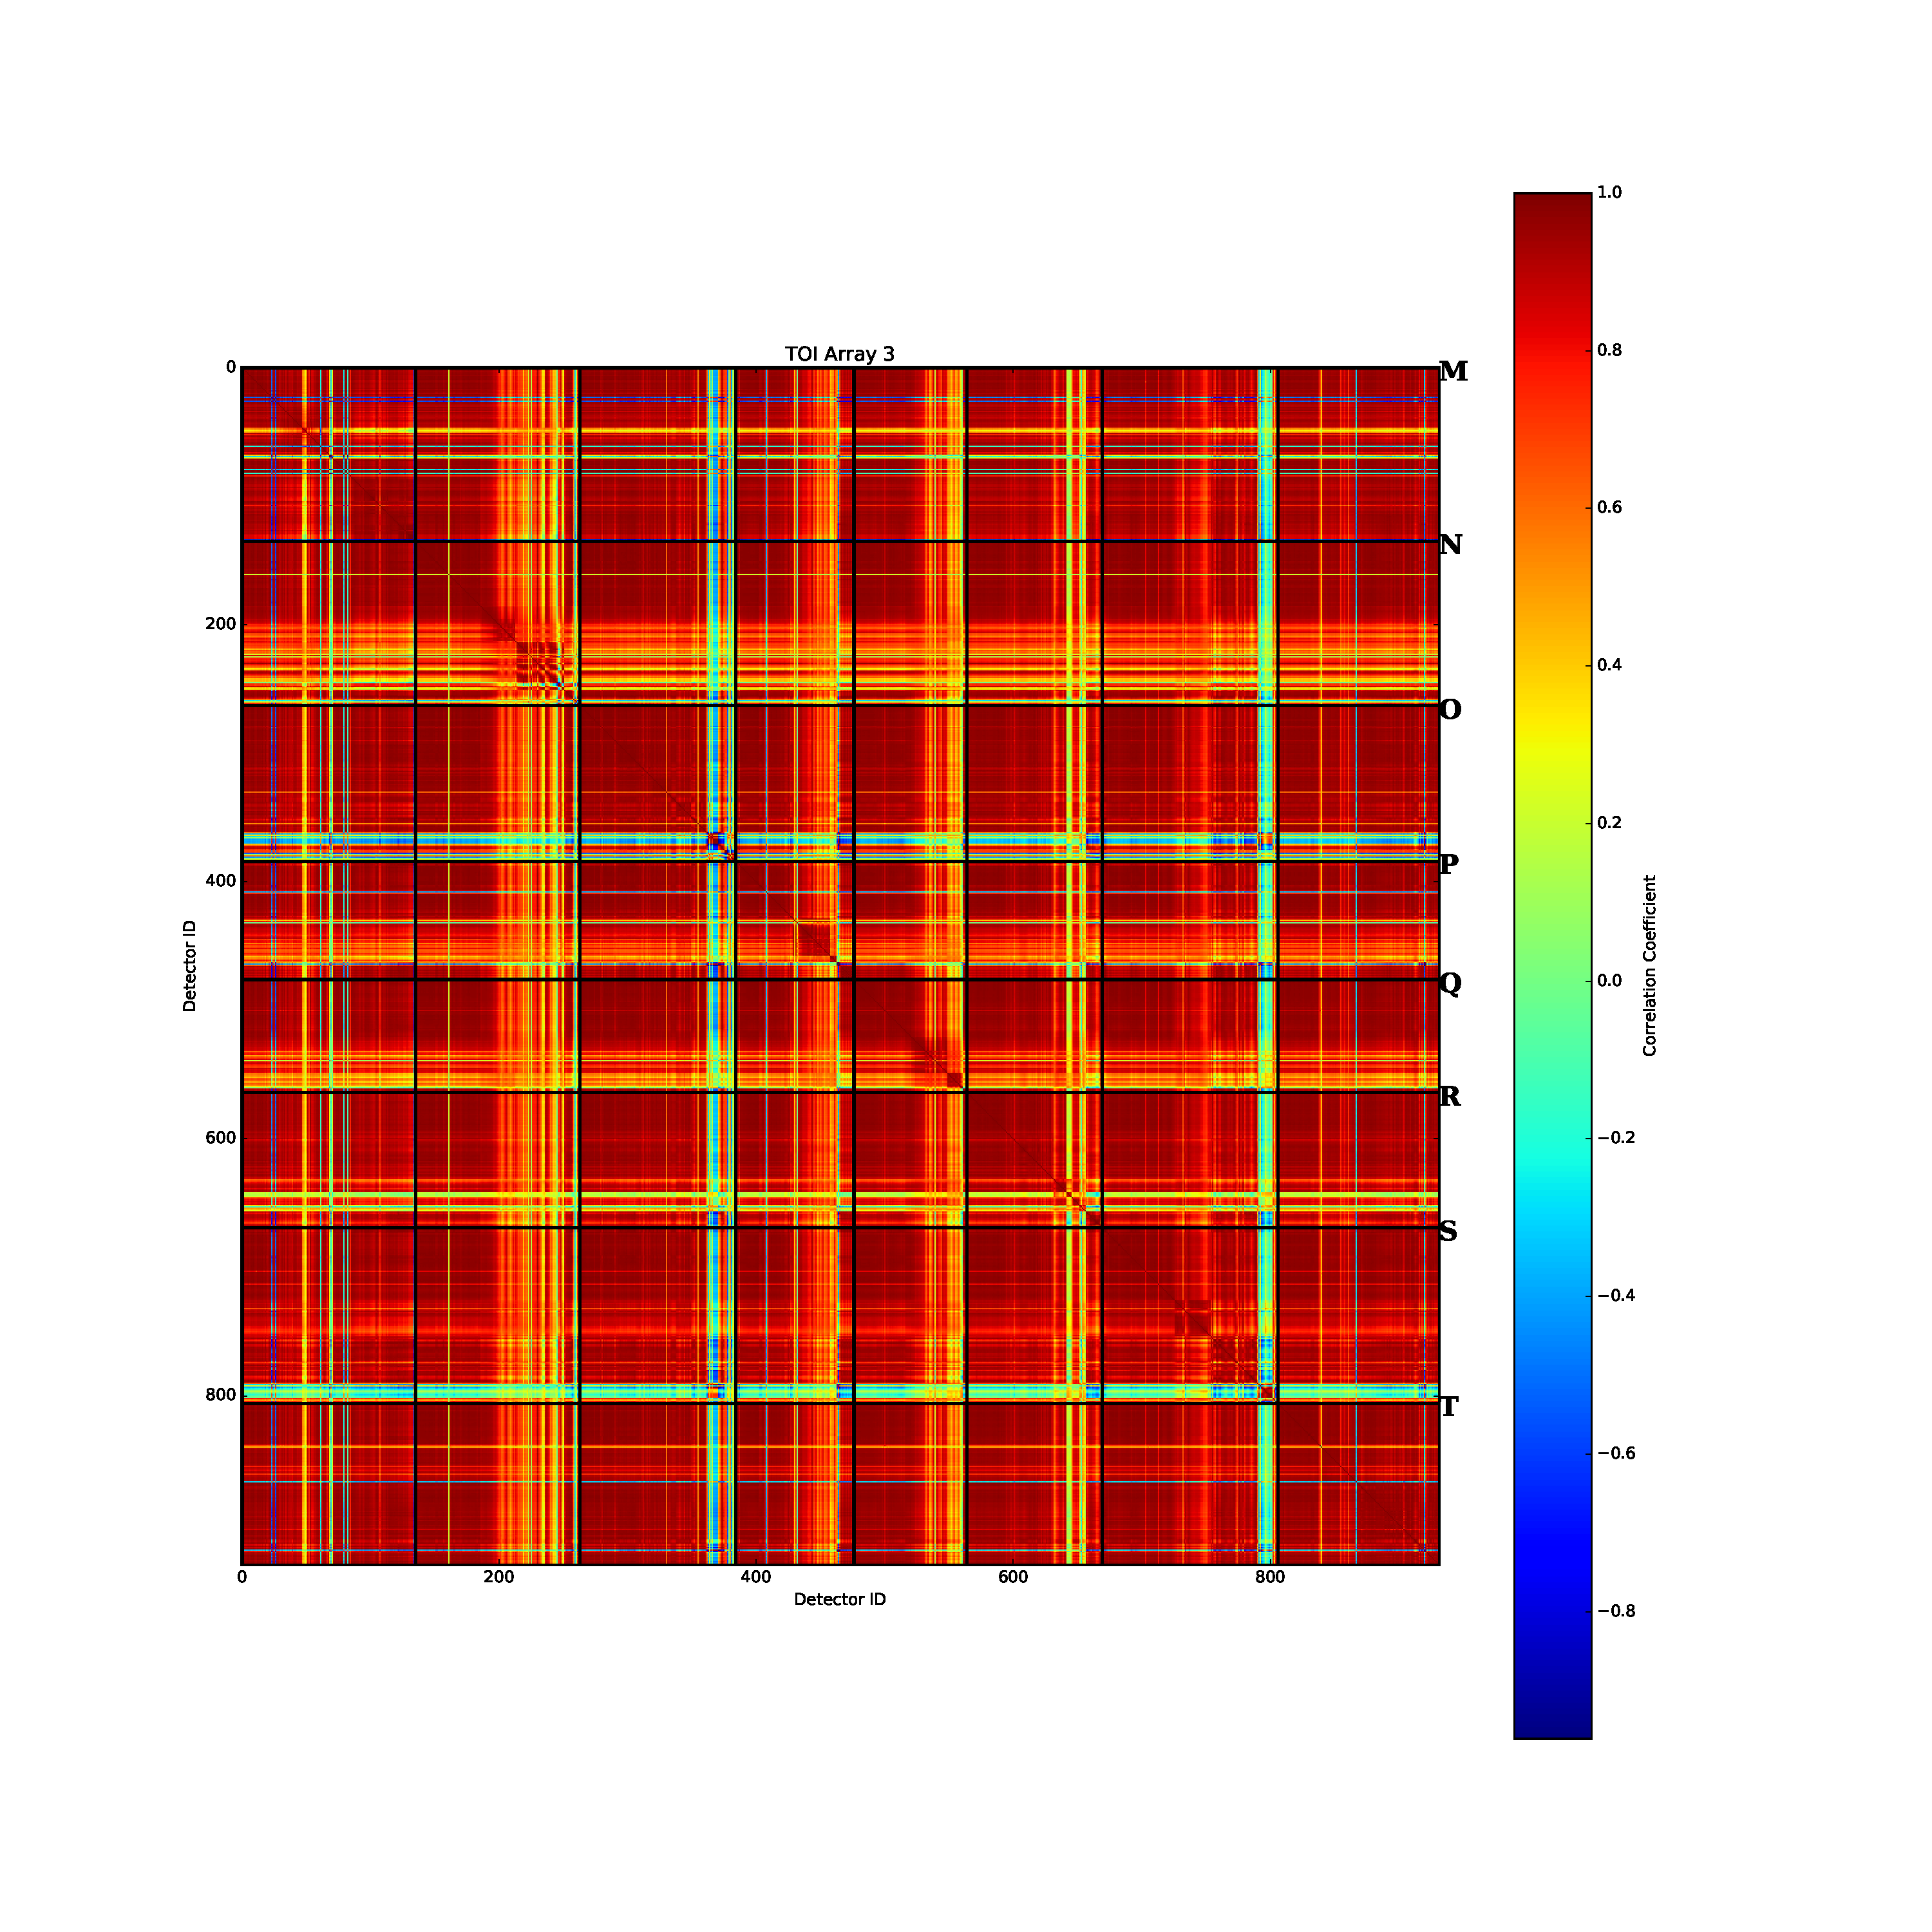
\includegraphics[width=0.3\textwidth]{Figures/DarkTests/corrmat_TOI_array_3_20160504s97.pdf}
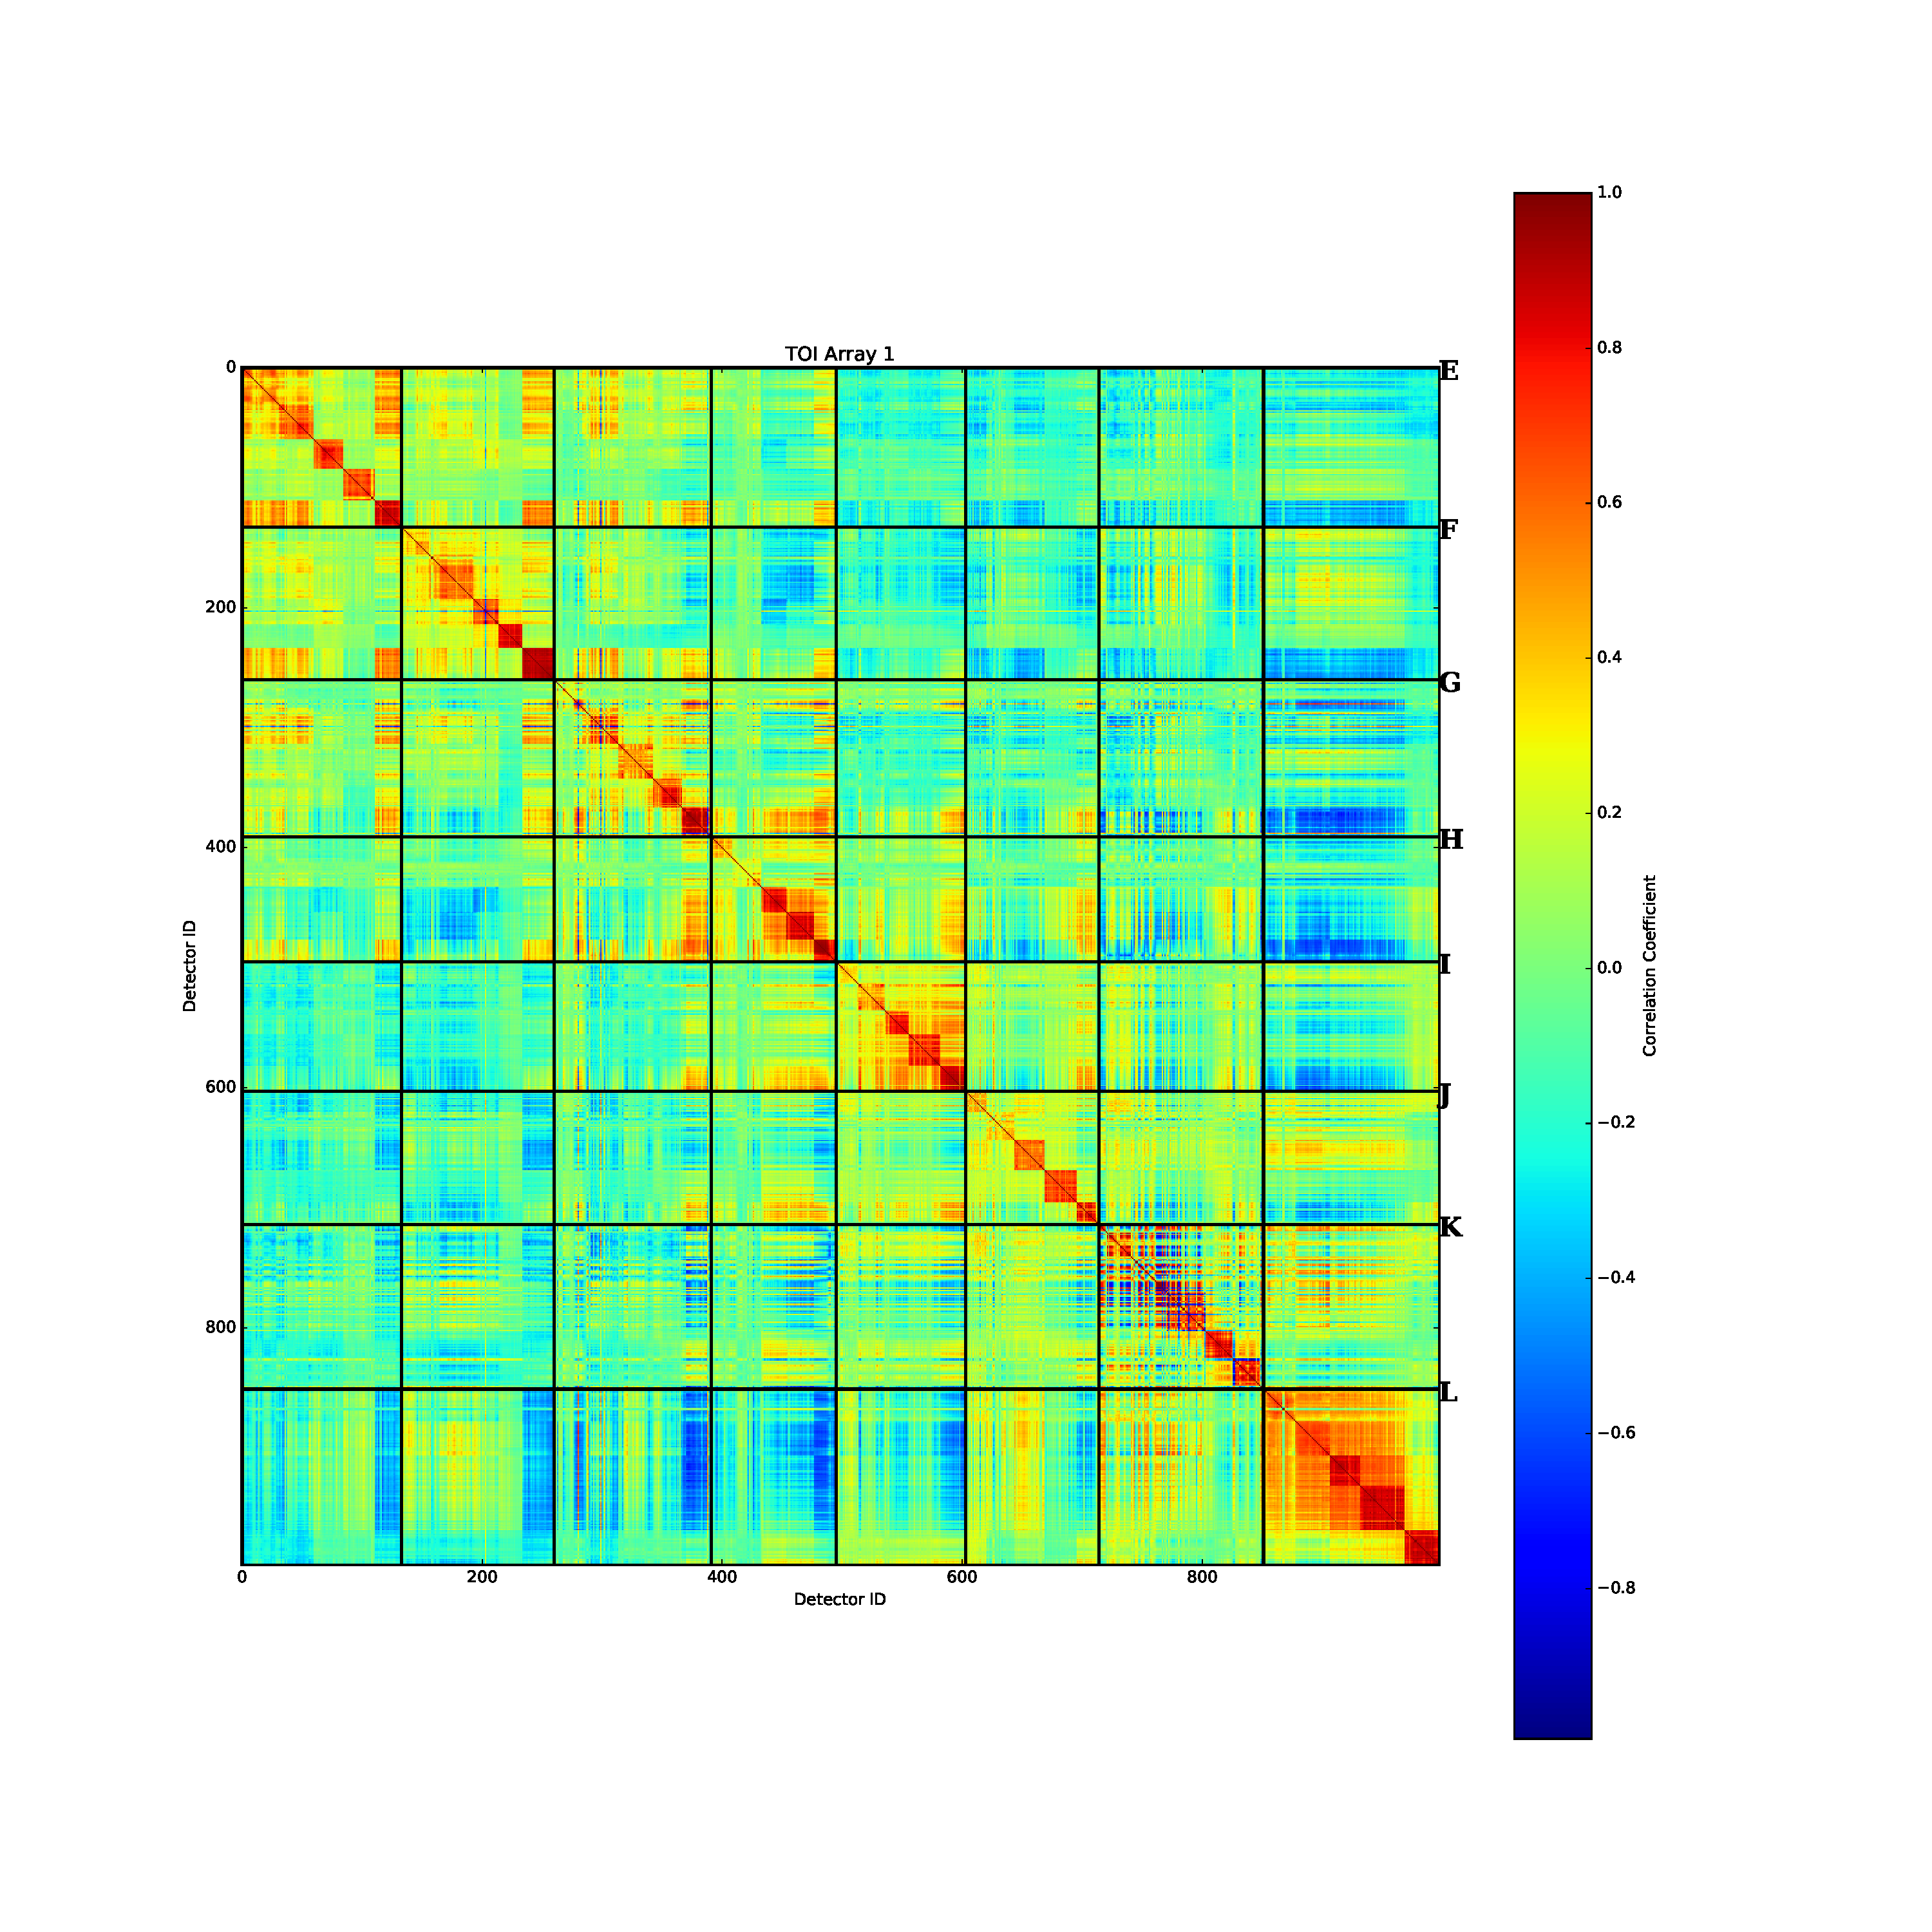
\includegraphics[width=0.3\textwidth]{Figures/DarkTests/corrmat_TOI_CM_array_1_20160504s97.pdf}
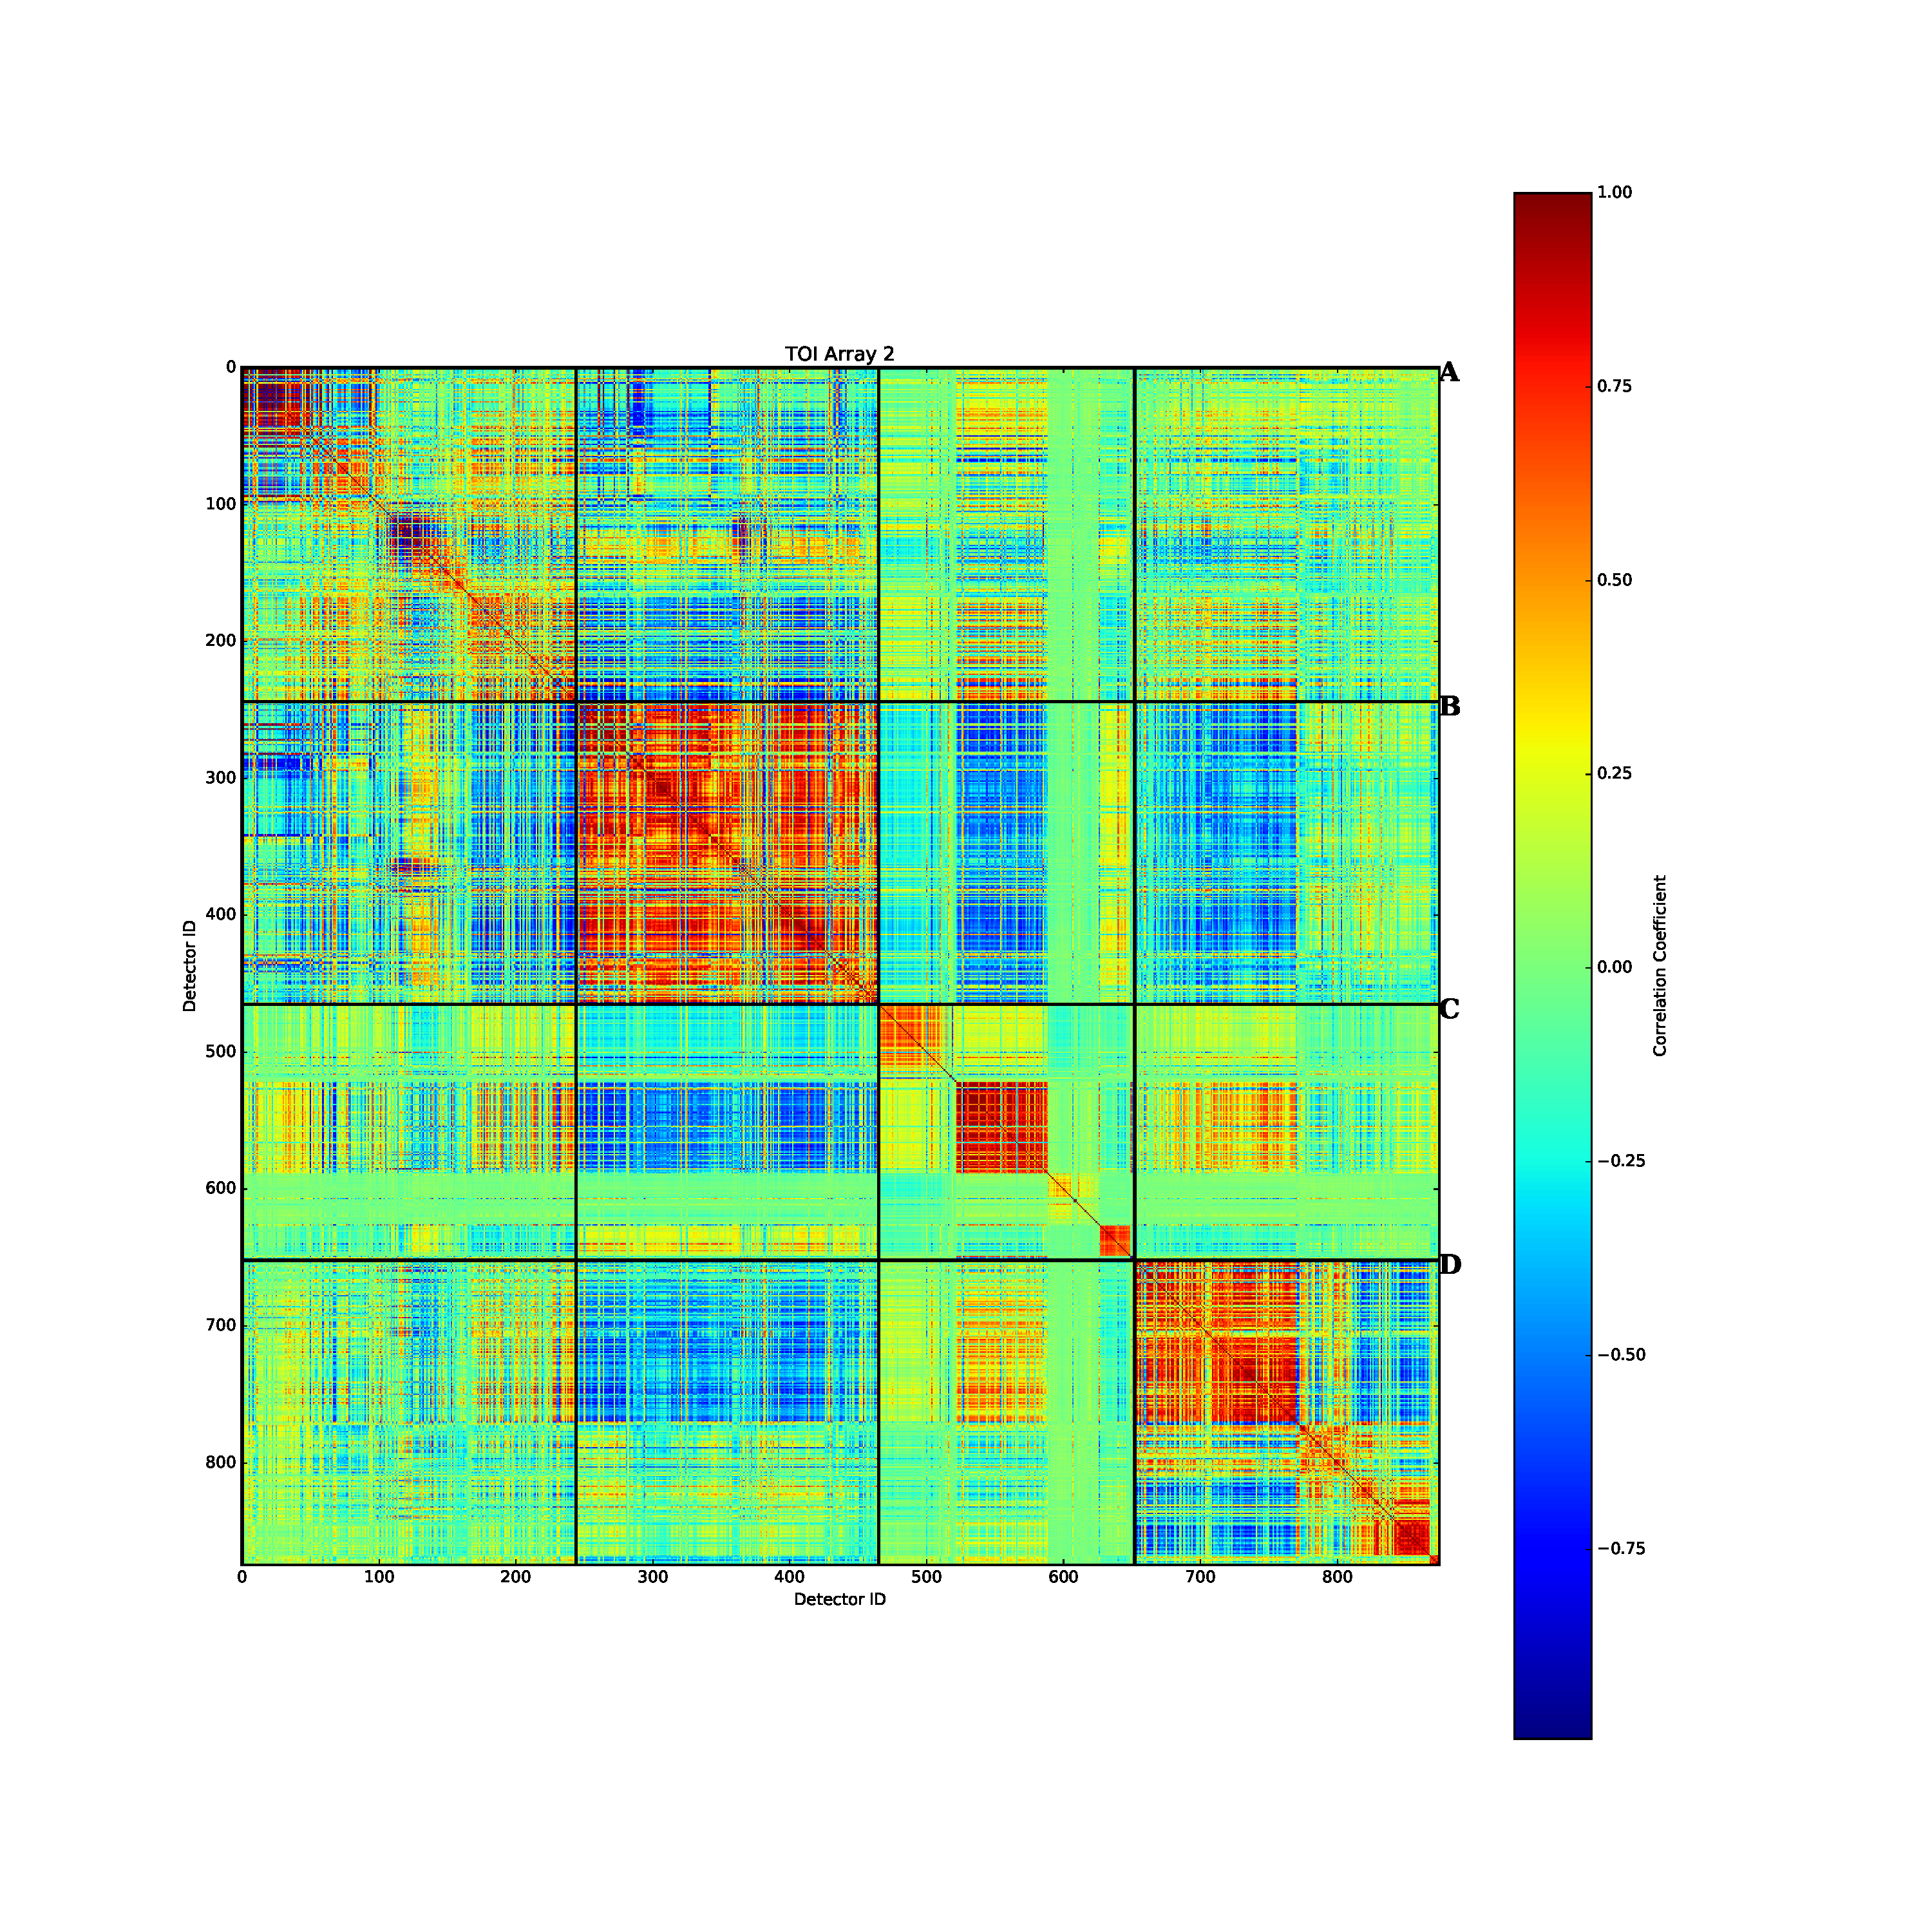
\includegraphics[width=0.3\textwidth]{Figures/DarkTests/corrmat_TOI_CM_array_2_20160504s97.pdf}
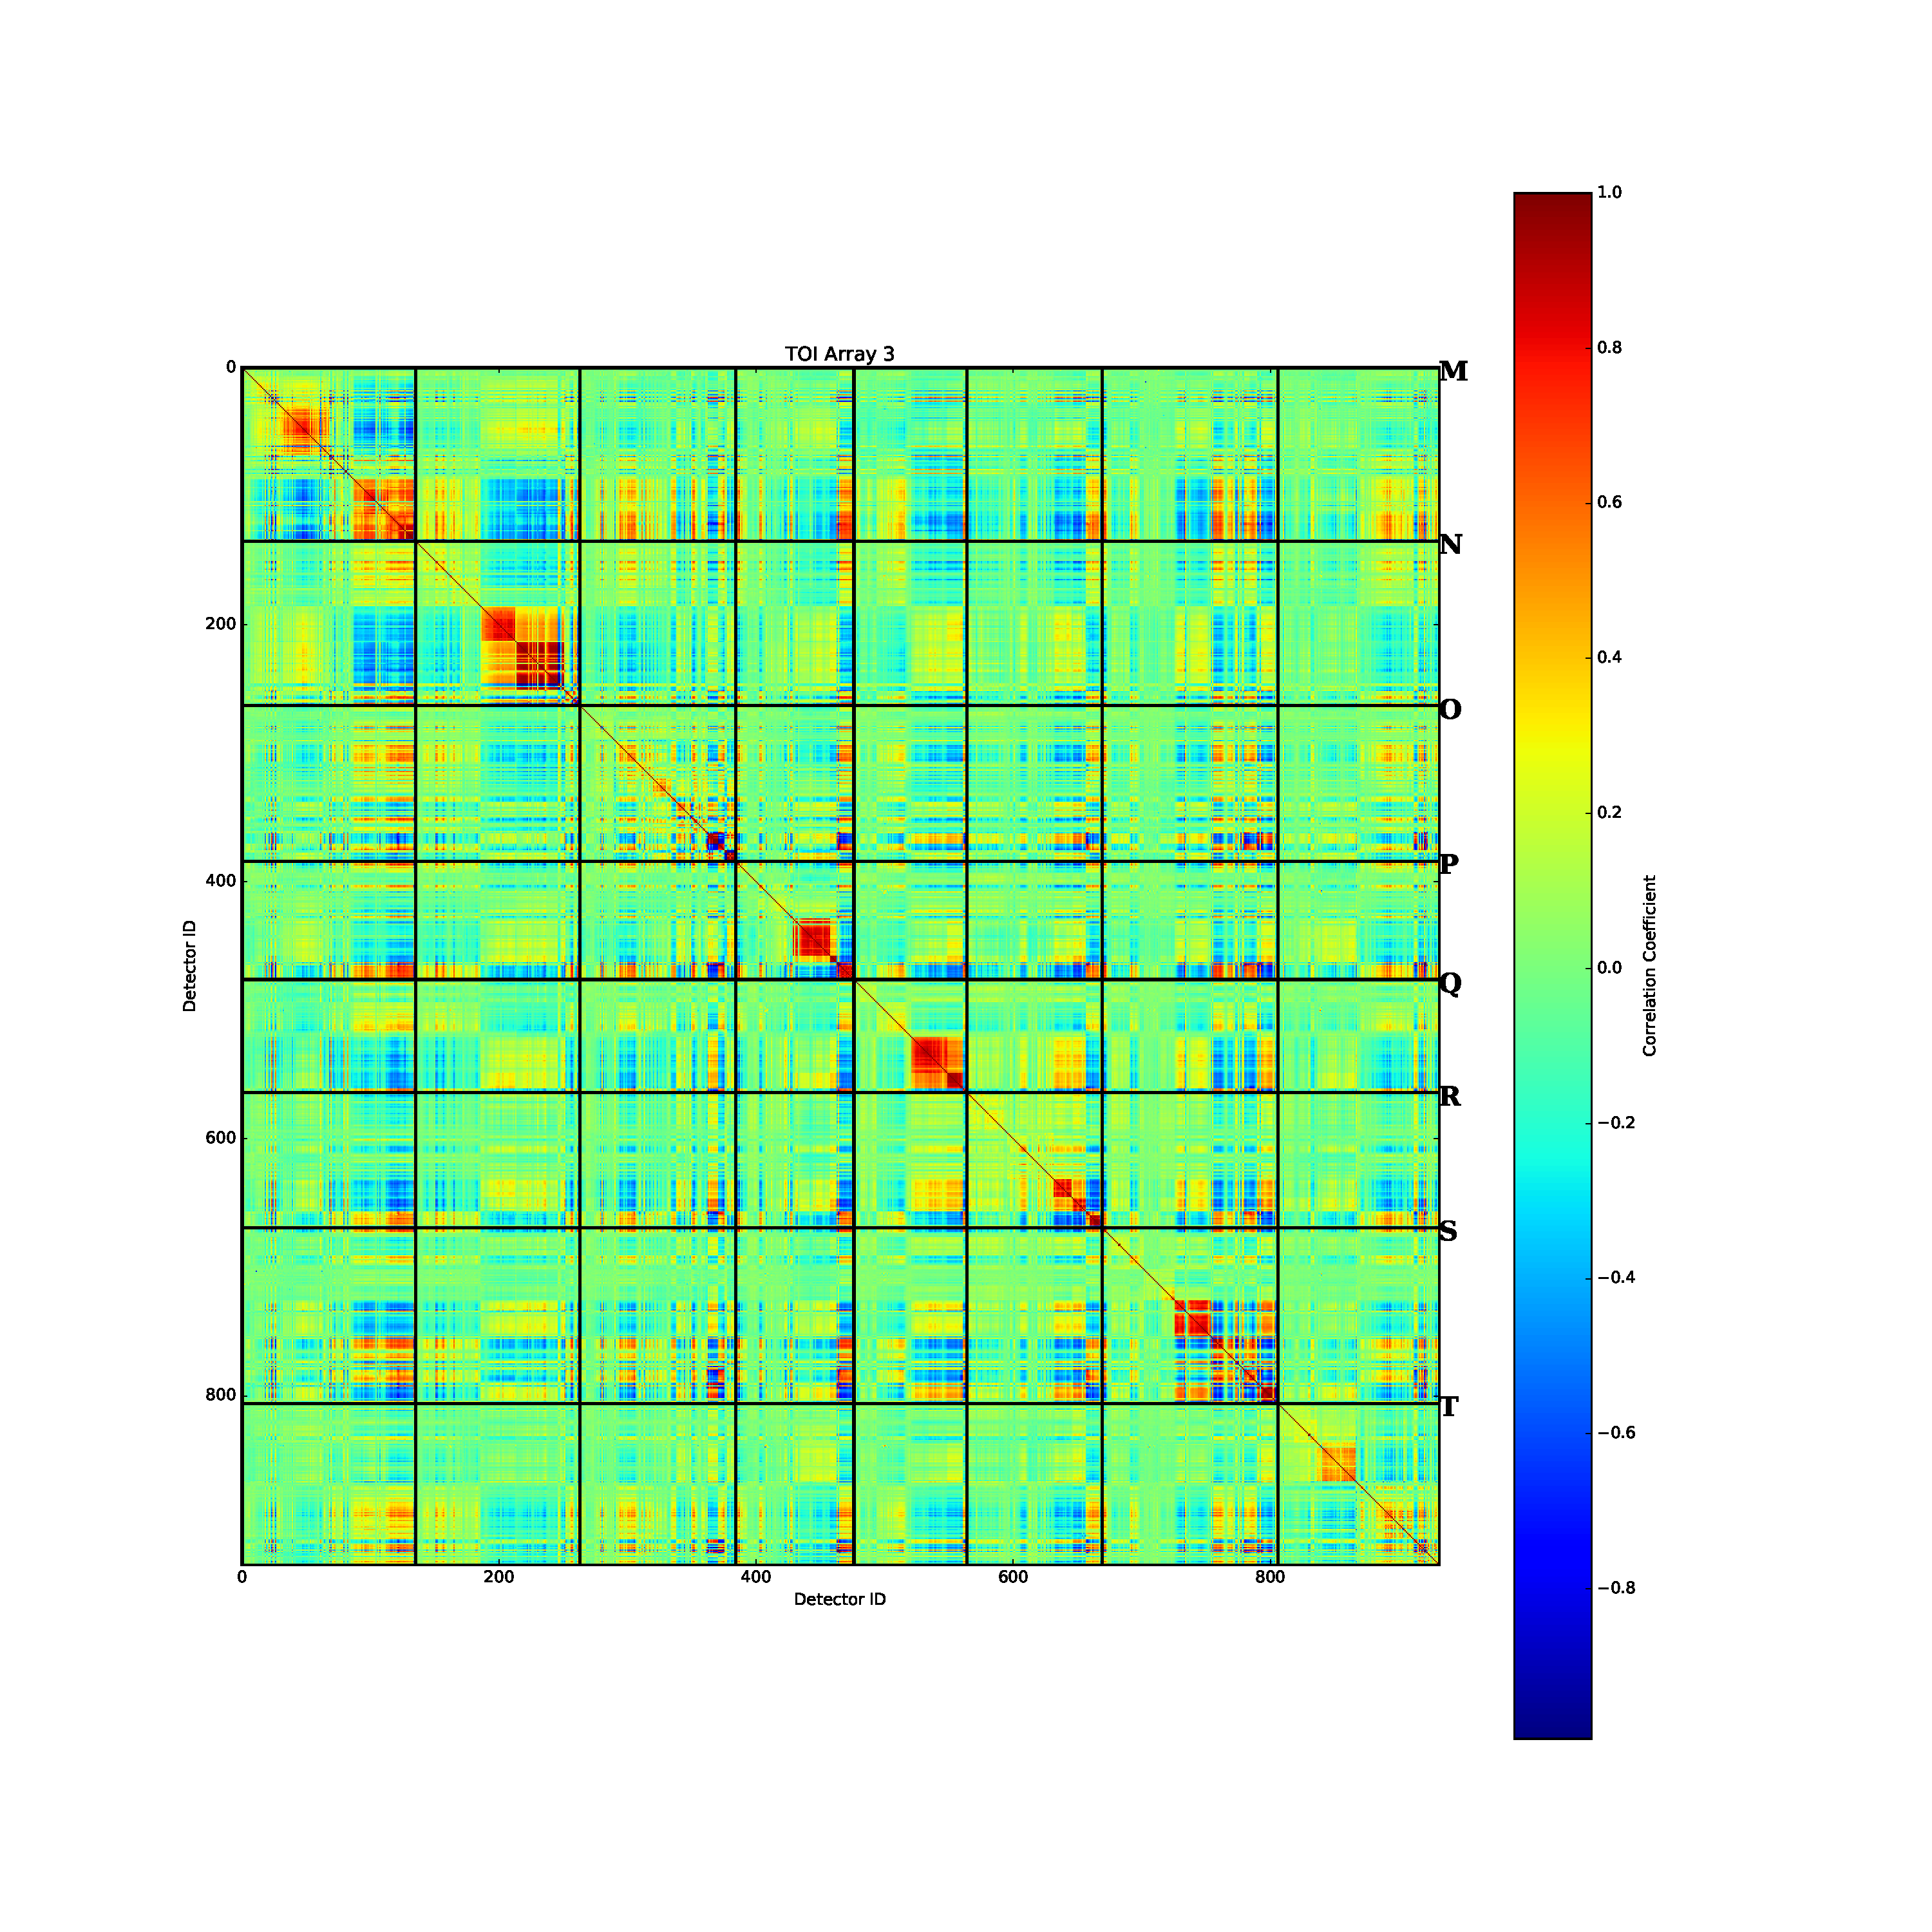
\includegraphics[width=0.3\textwidth]{Figures/DarkTests/corrmat_TOI_CM_array_3_20160504s97.pdf}
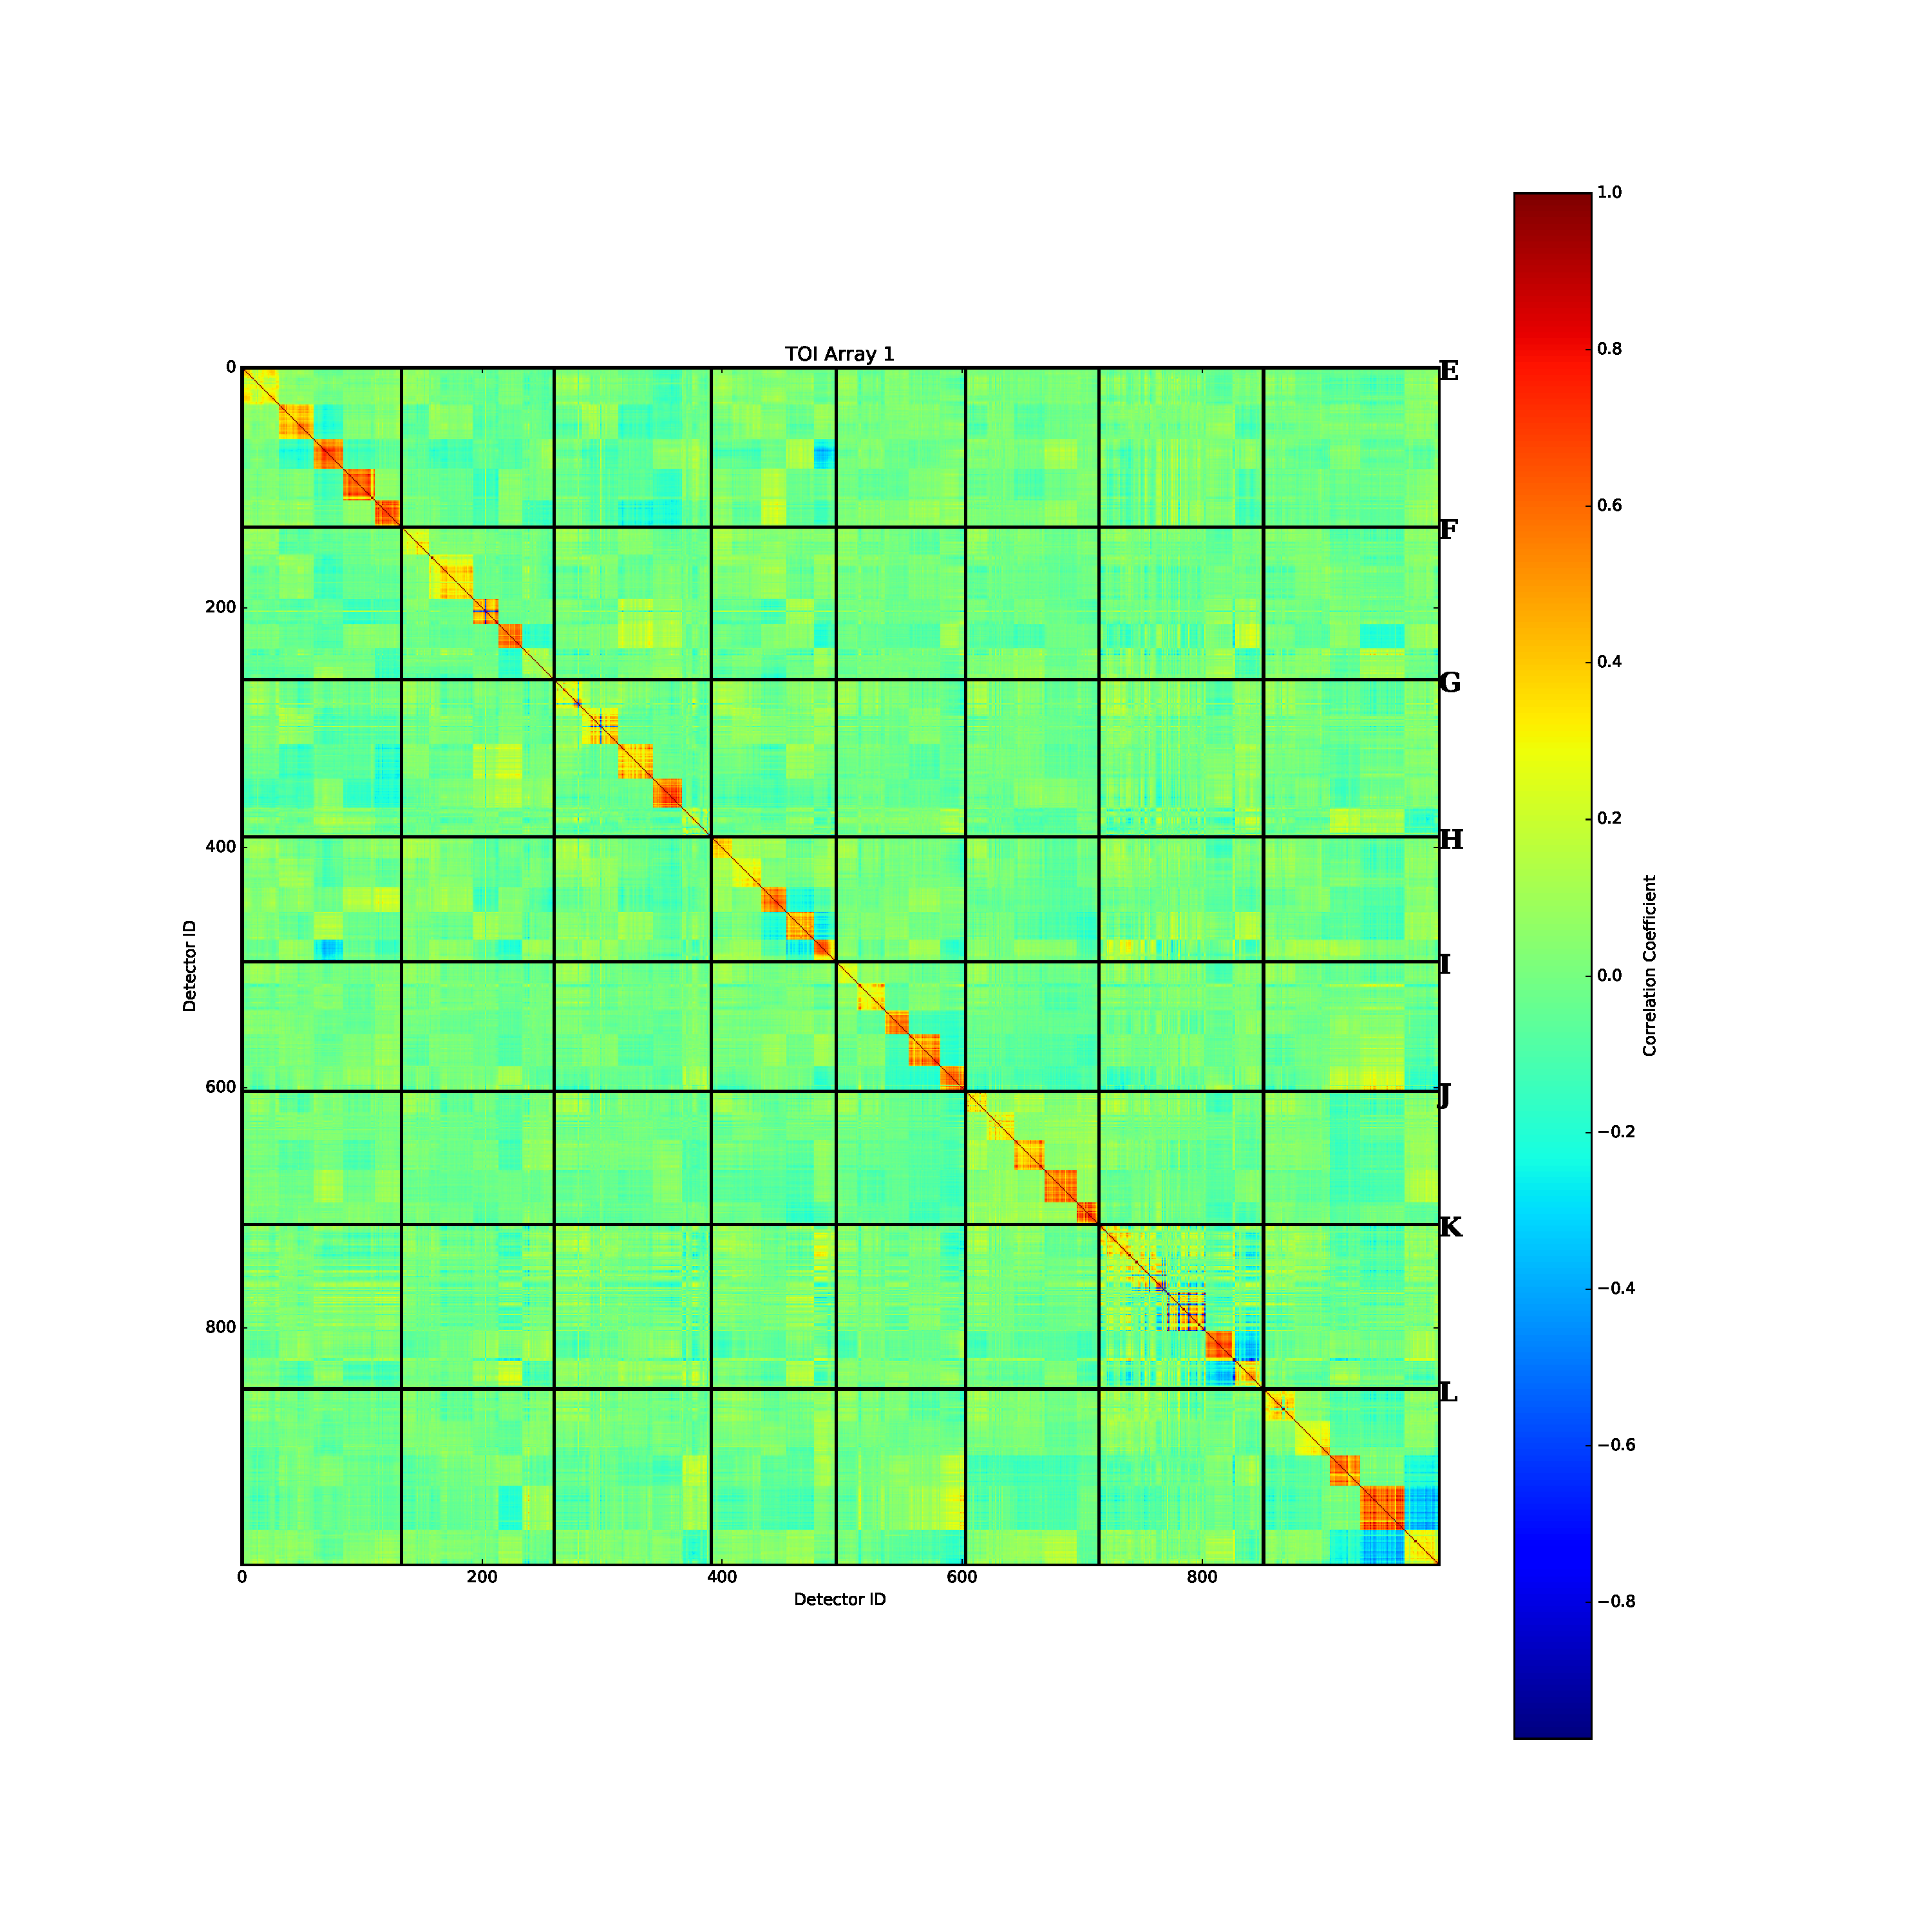
\includegraphics[width=0.3\textwidth]{Figures/DarkTests/corrmat_TOI_PCA_array_1_20160504s97.pdf}
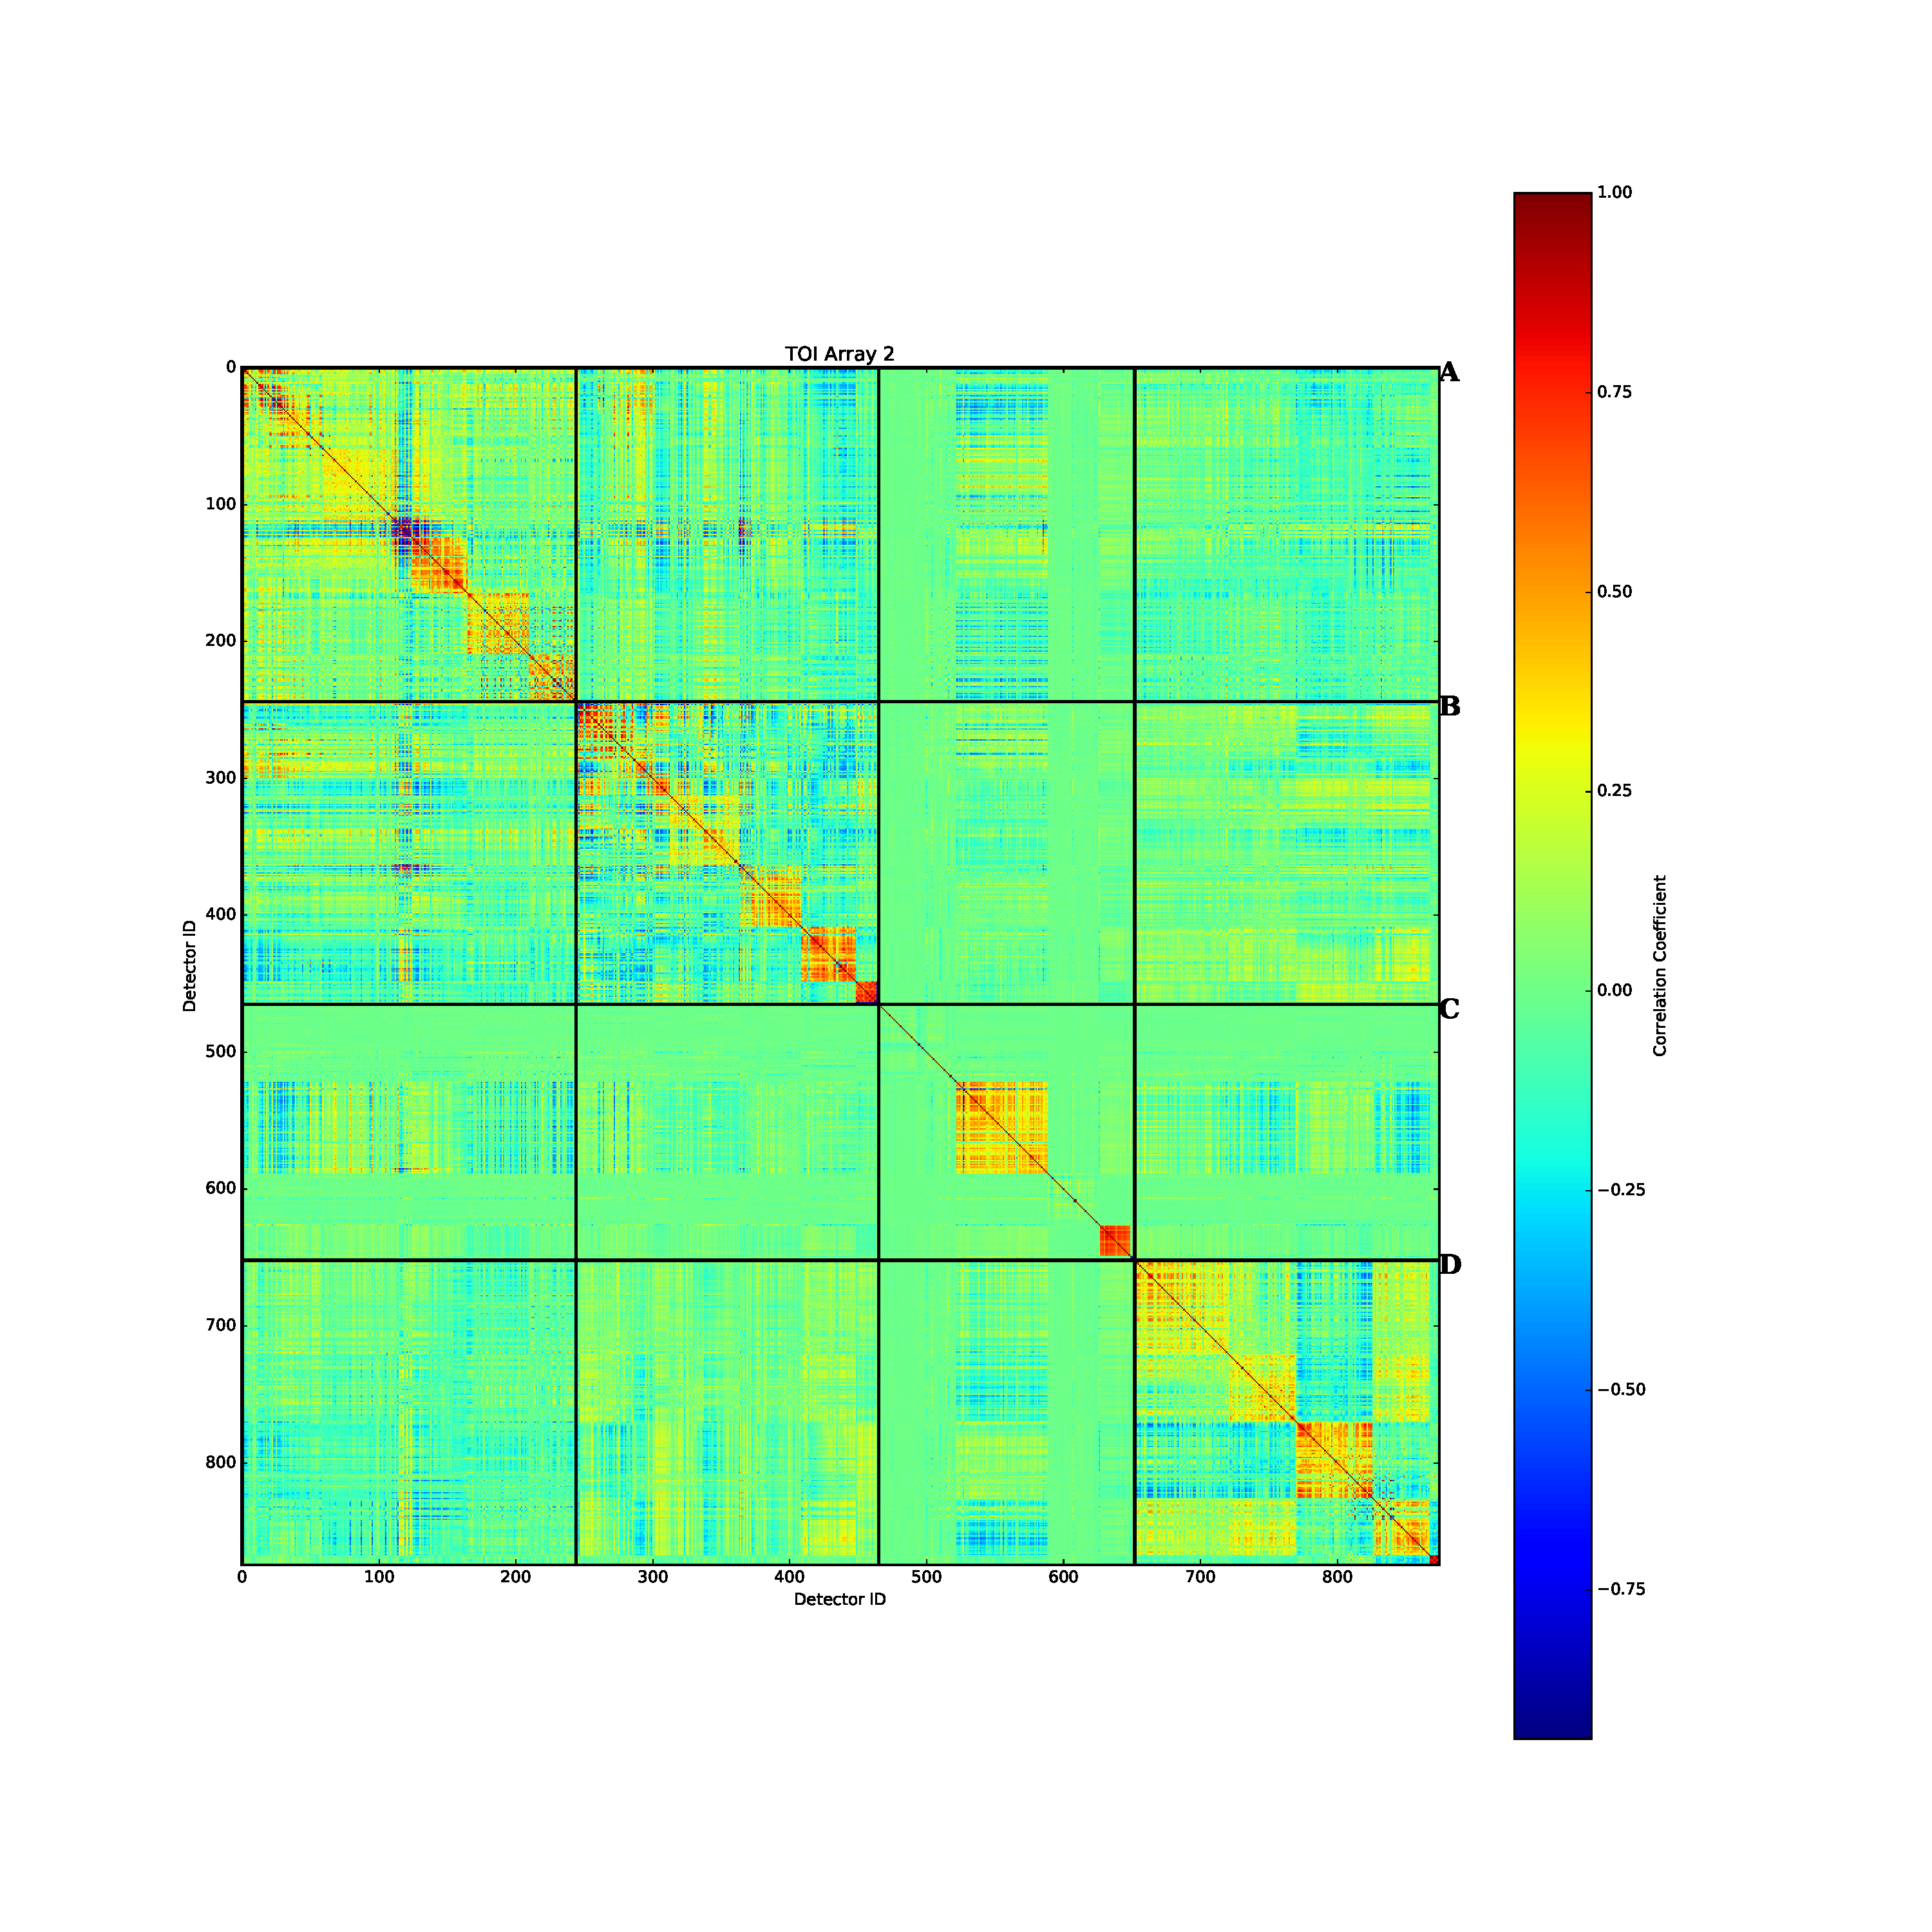
\includegraphics[width=0.3\textwidth]{Figures/DarkTests/corrmat_TOI_PCA_array_2_20160504s97.pdf}
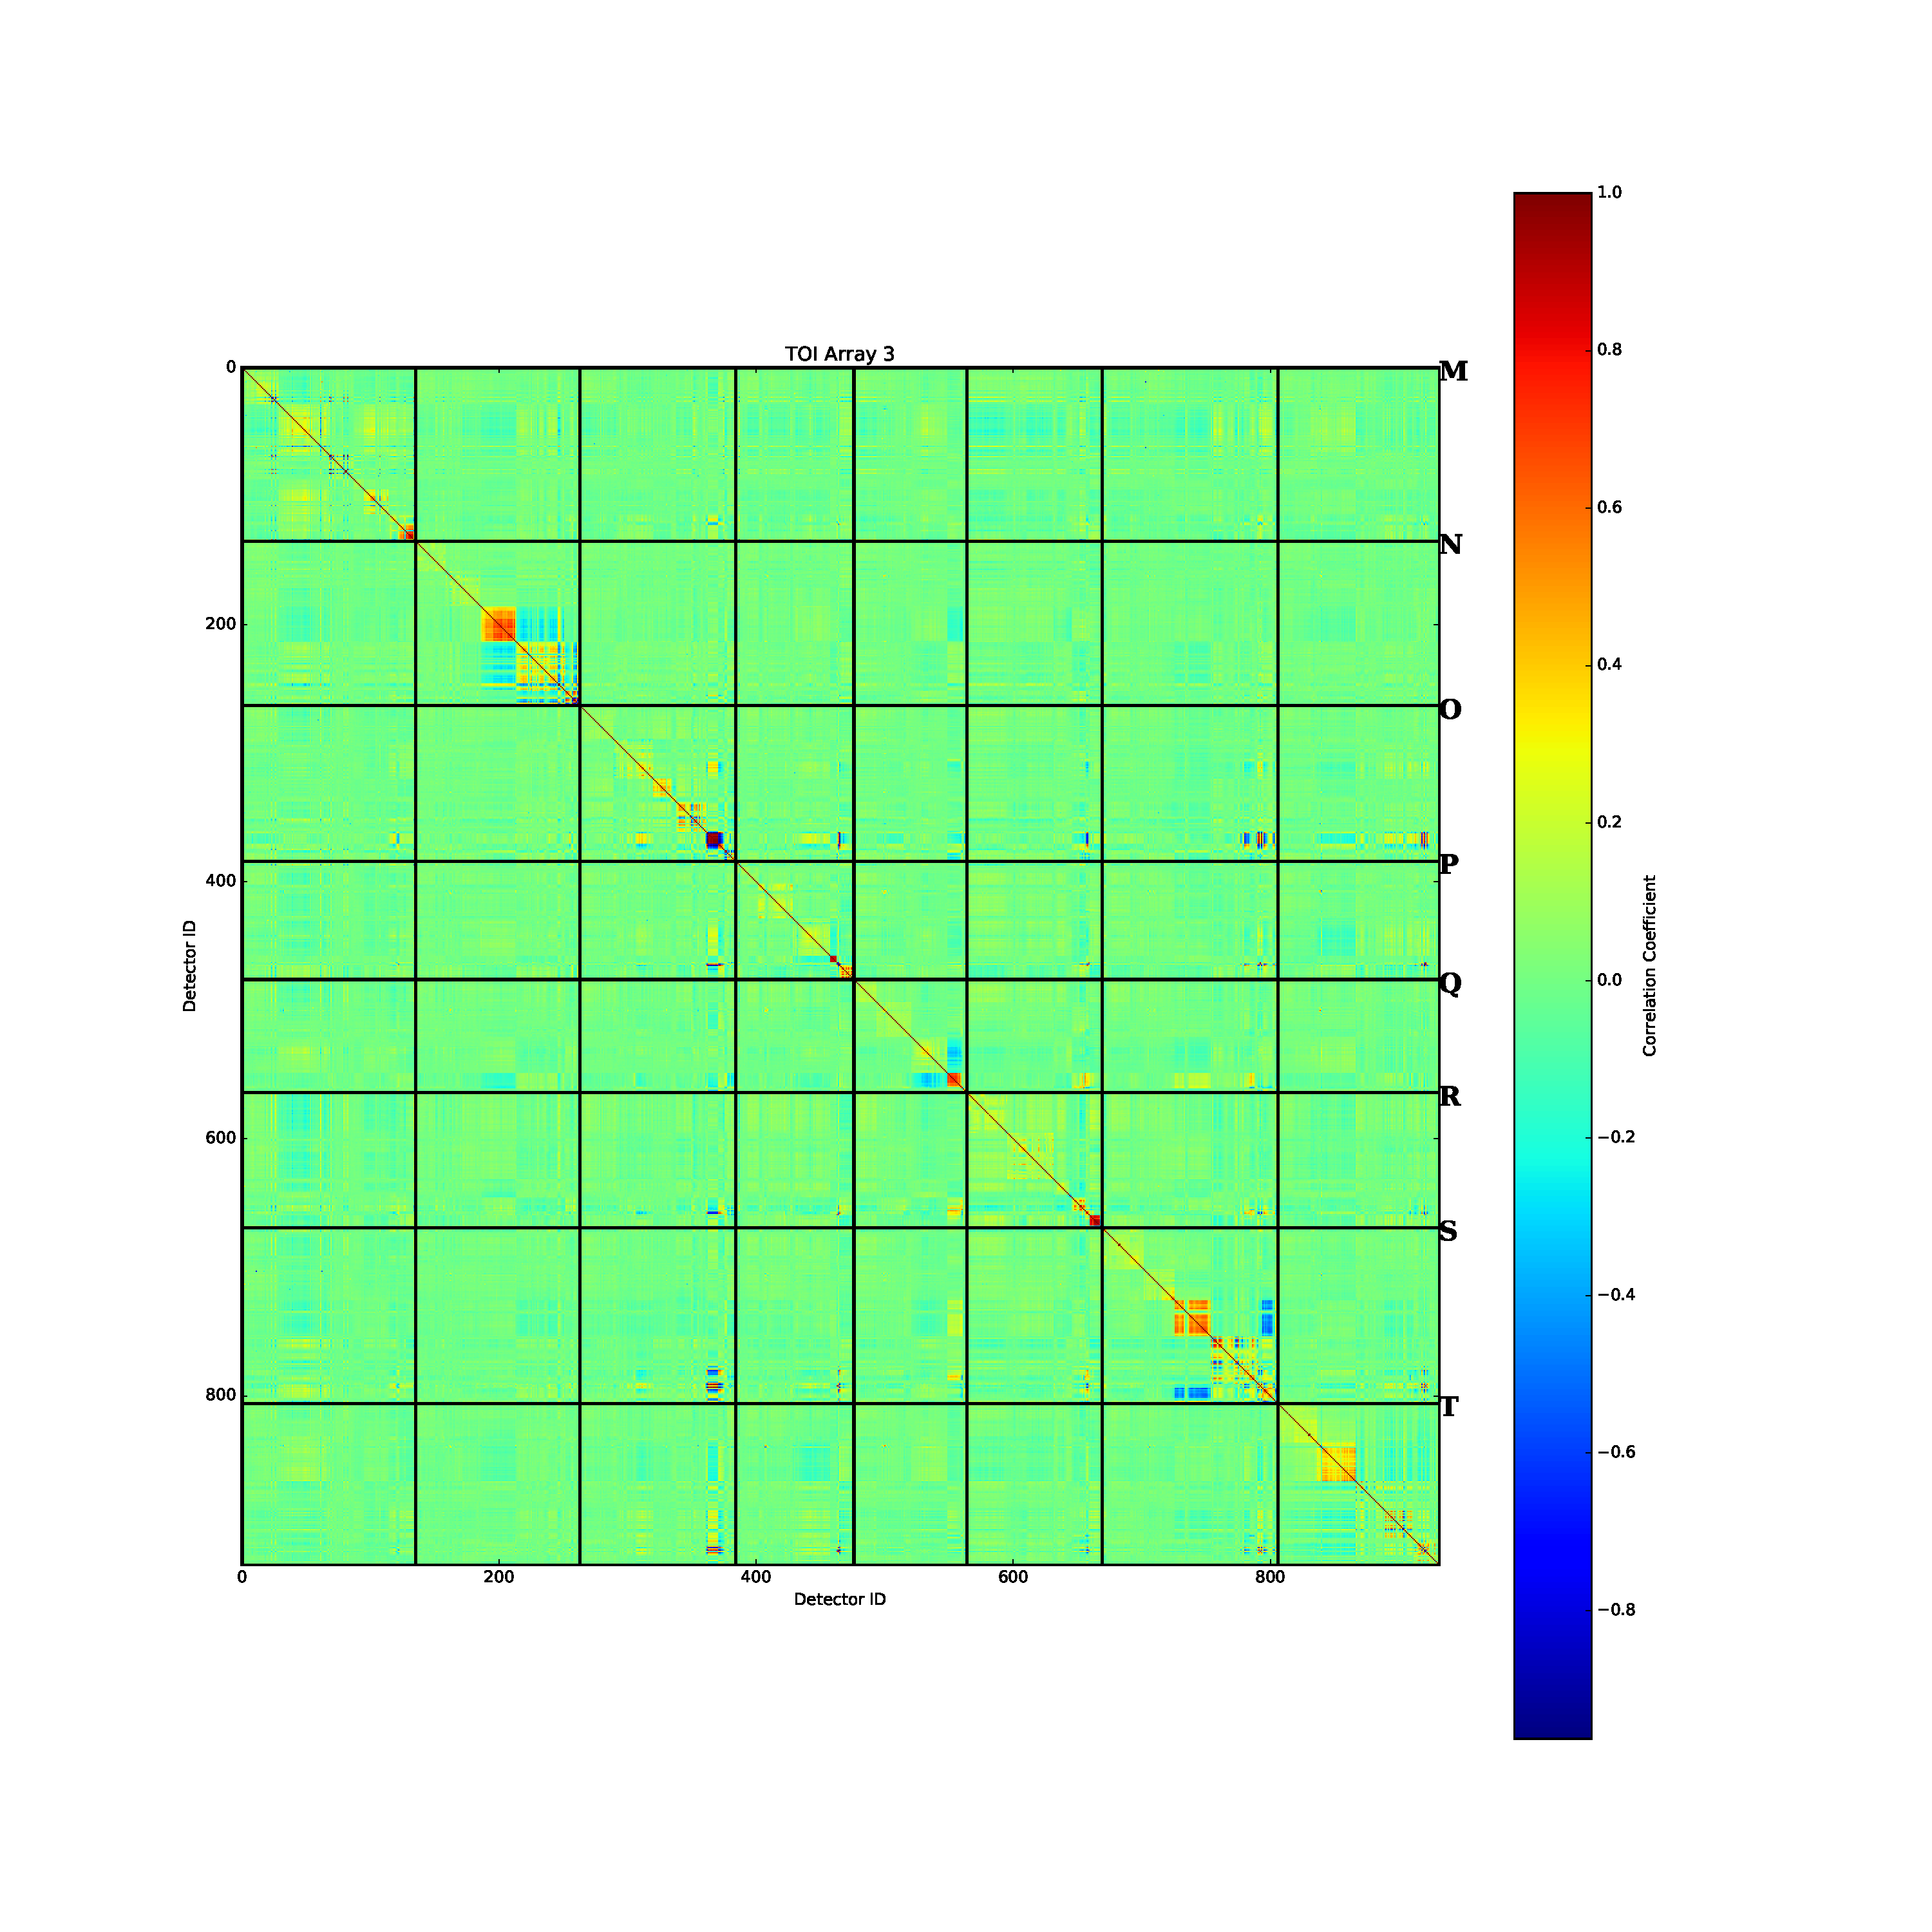
\includegraphics[width=0.3\textwidth]{Figures/DarkTests/corrmat_TOI_PCA_array_3_20160504s97.pdf}
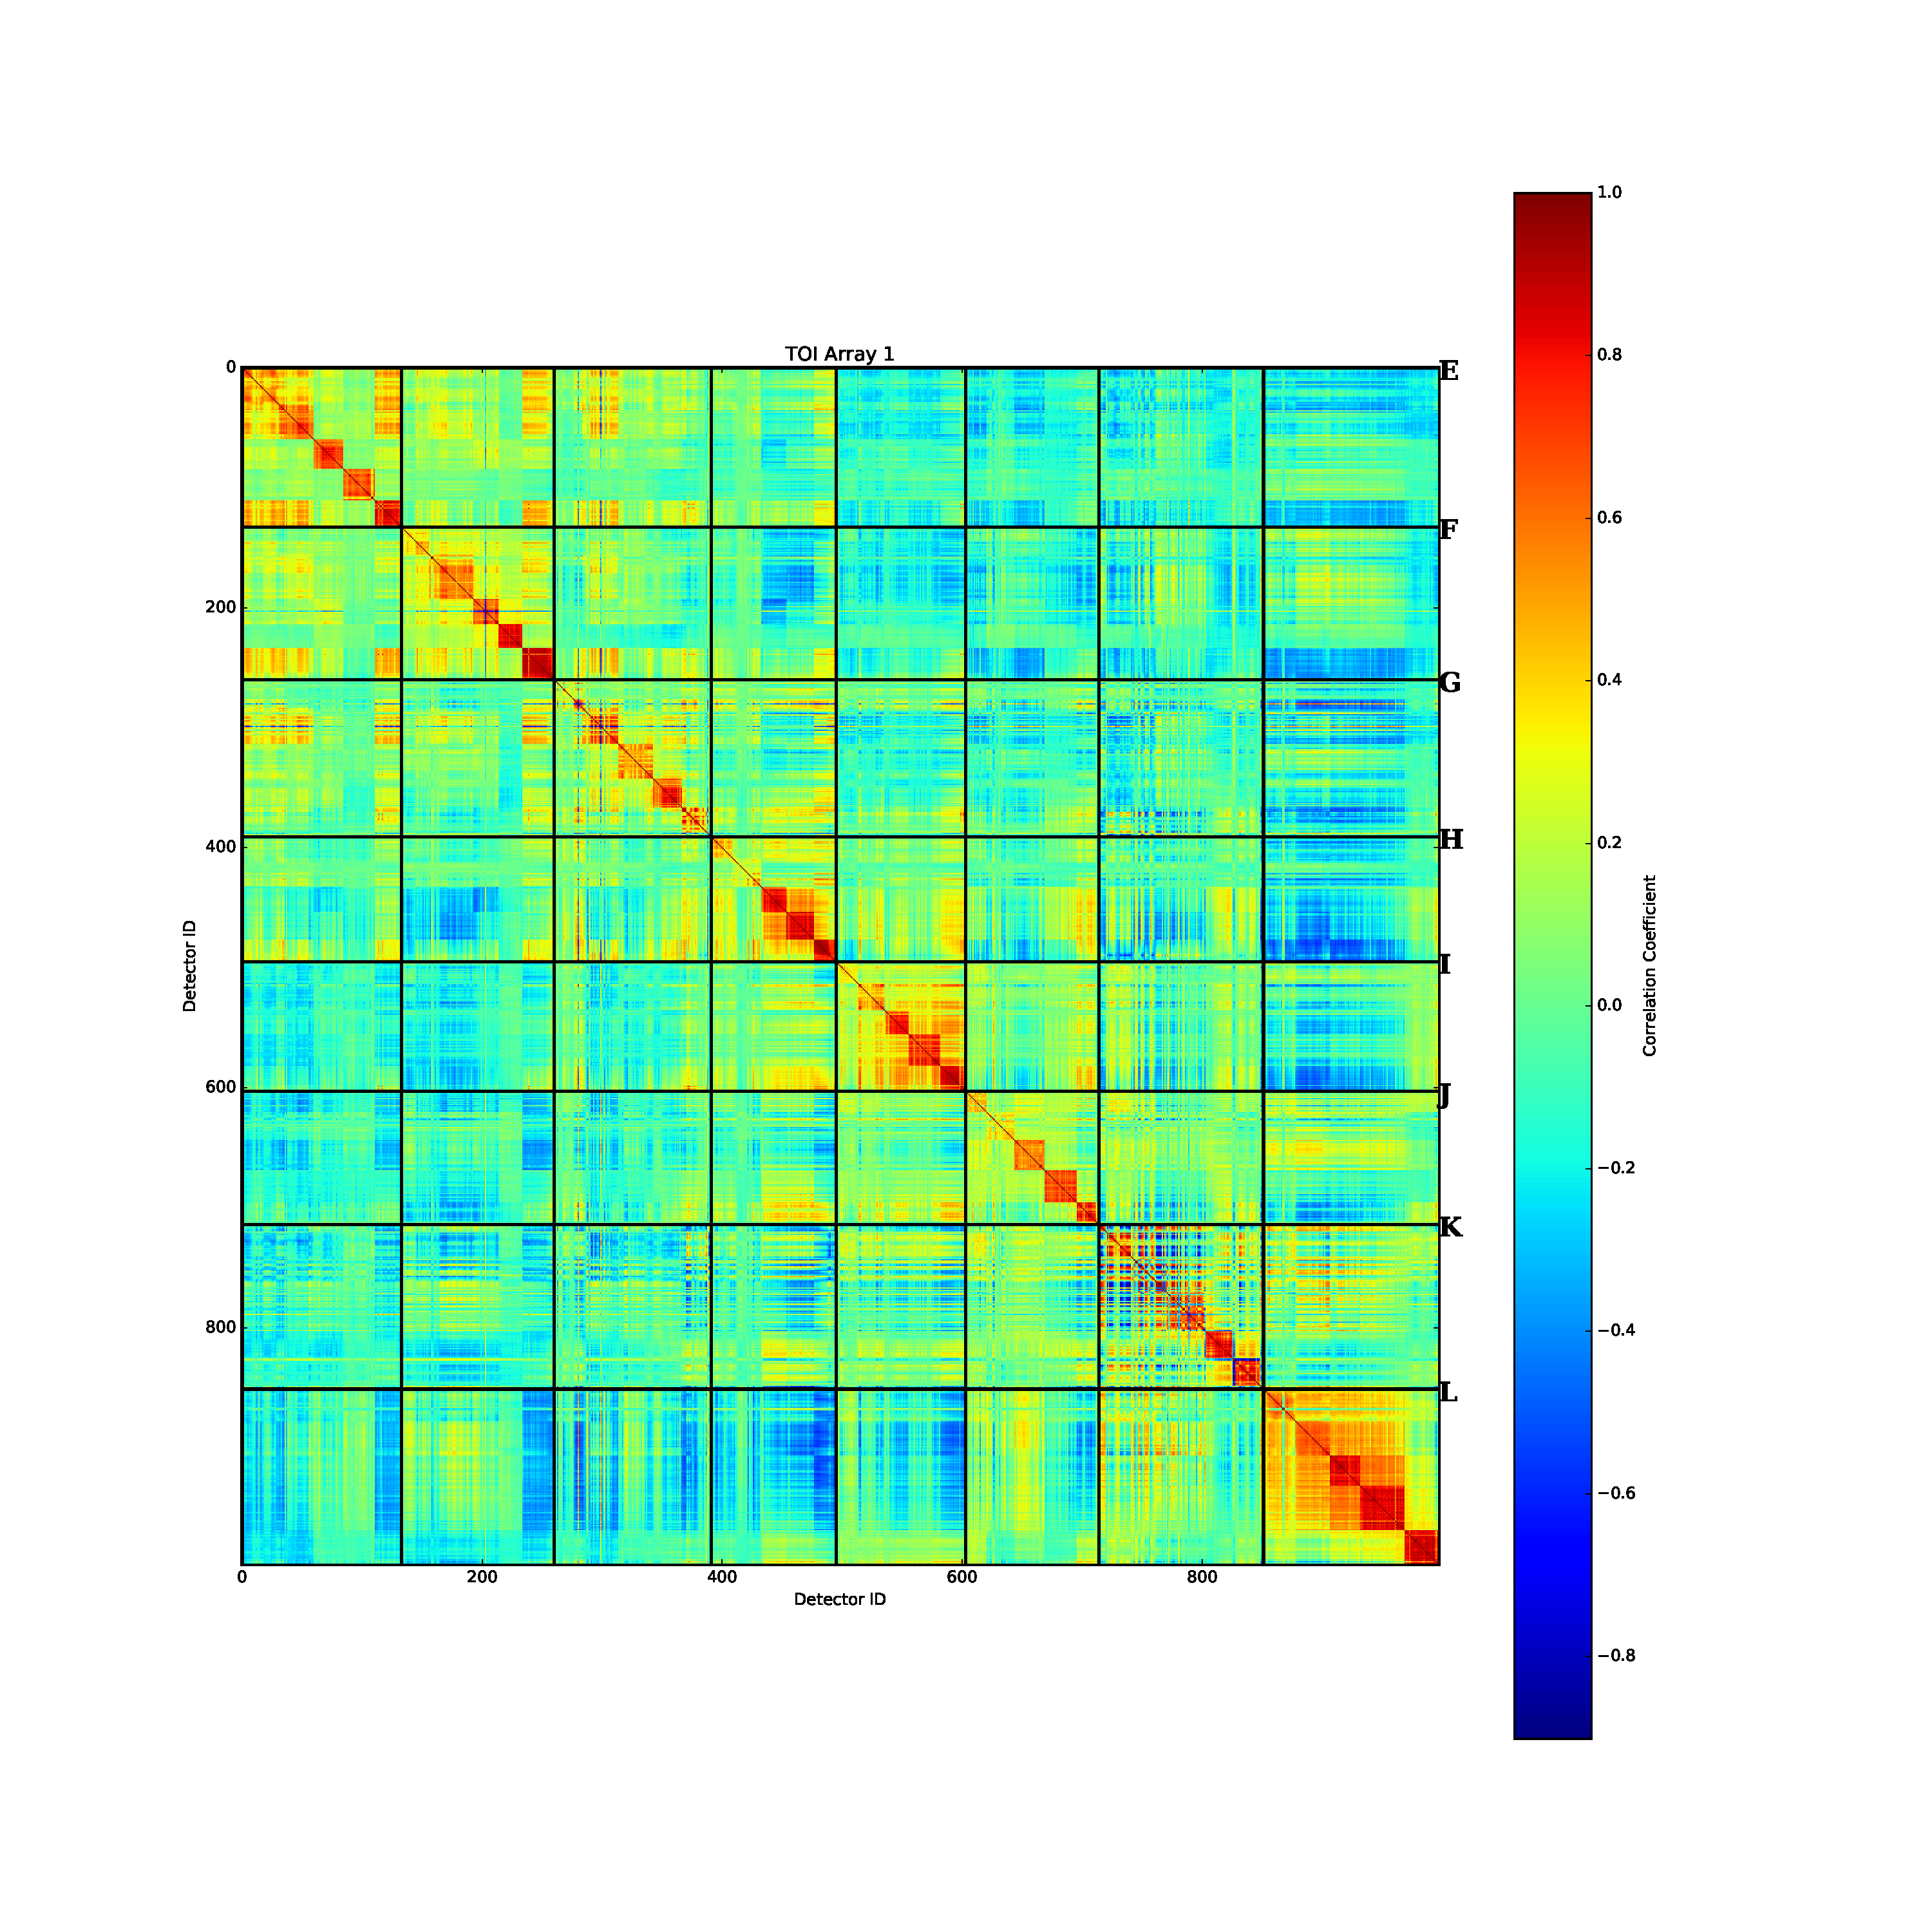
\includegraphics[width=0.3\textwidth]{Figures/DarkTests/corrmat_TOI_BC_array_1_20160504s97.pdf}
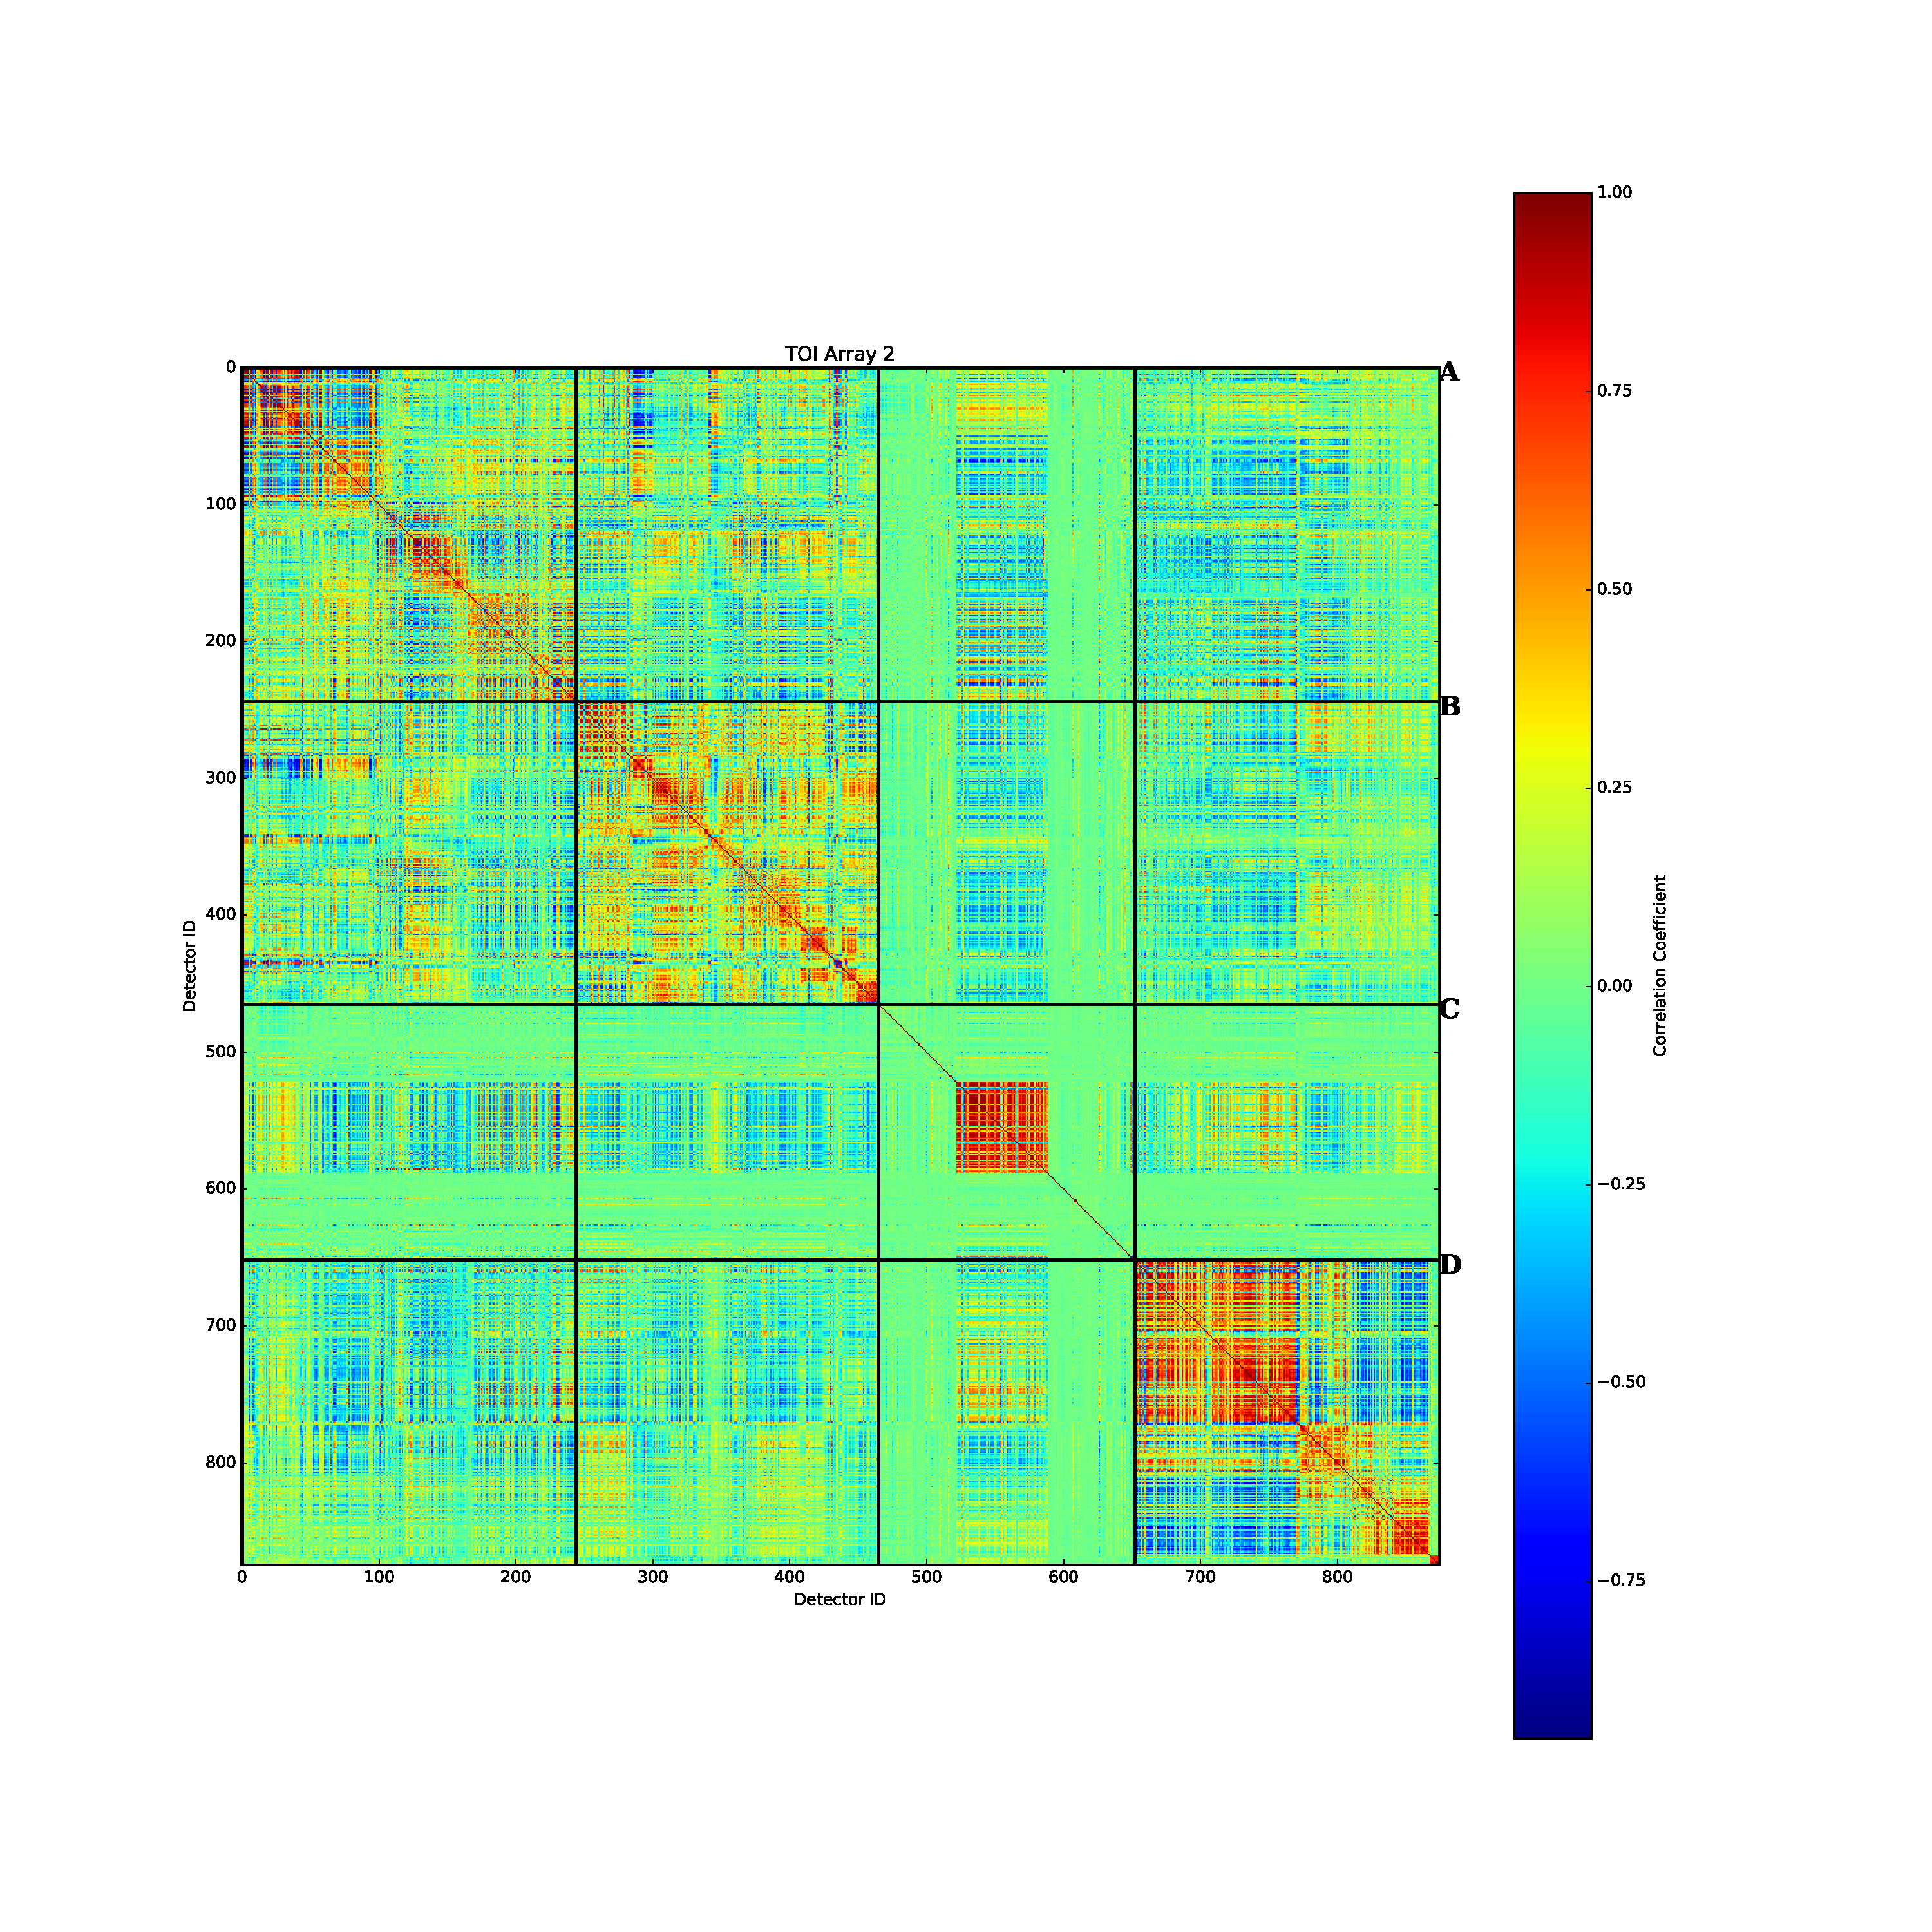
\includegraphics[width=0.3\textwidth]{Figures/DarkTests/corrmat_TOI_BC_array_2_20160504s97.pdf}
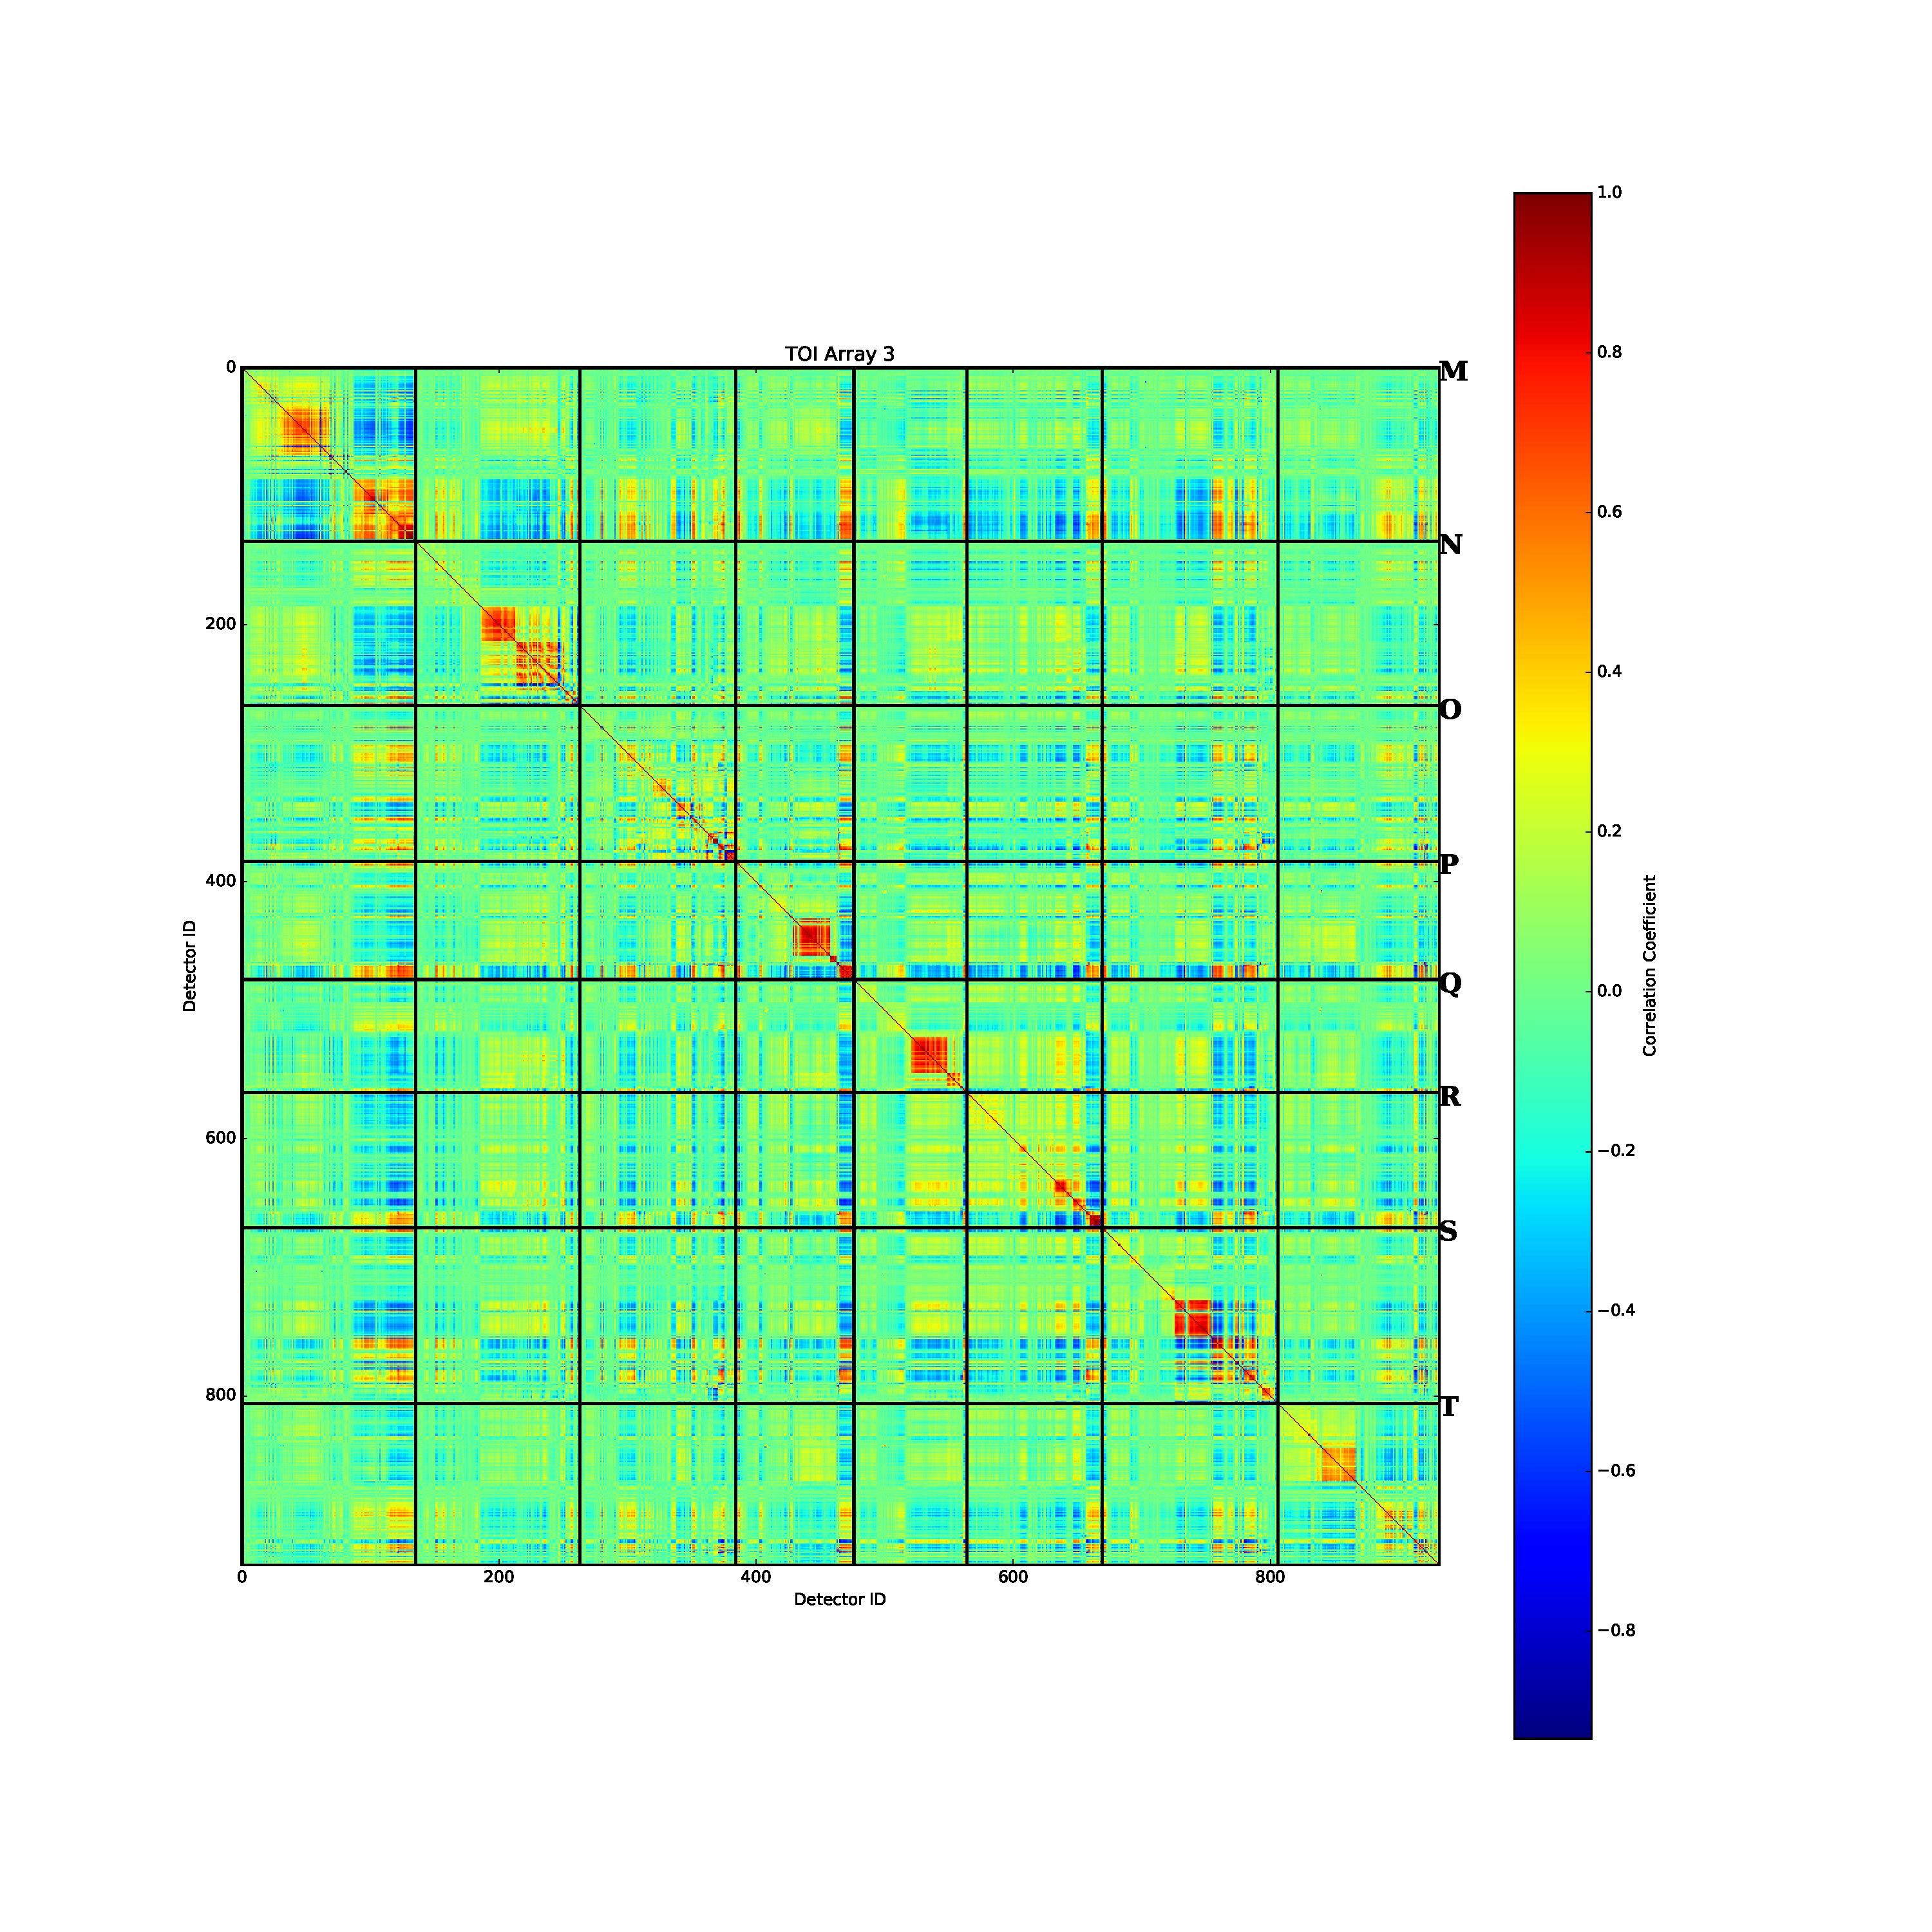
\includegraphics[width=0.3\textwidth]{Figures/DarkTests/corrmat_TOI_BC_array_3_20160504s97.pdf}
\end{center}
\caption{From left to right correlation matrices for the three NIKA2 arrays (A1, A2, and A3) for scan 20160504s97. From top to bottom we present the correlation of the raw data, after CM, PCA and BC decorrelations. \label{corrs97}}
\end{figure}


\begin{figure}[ht] % Inline image example
\begin{center}
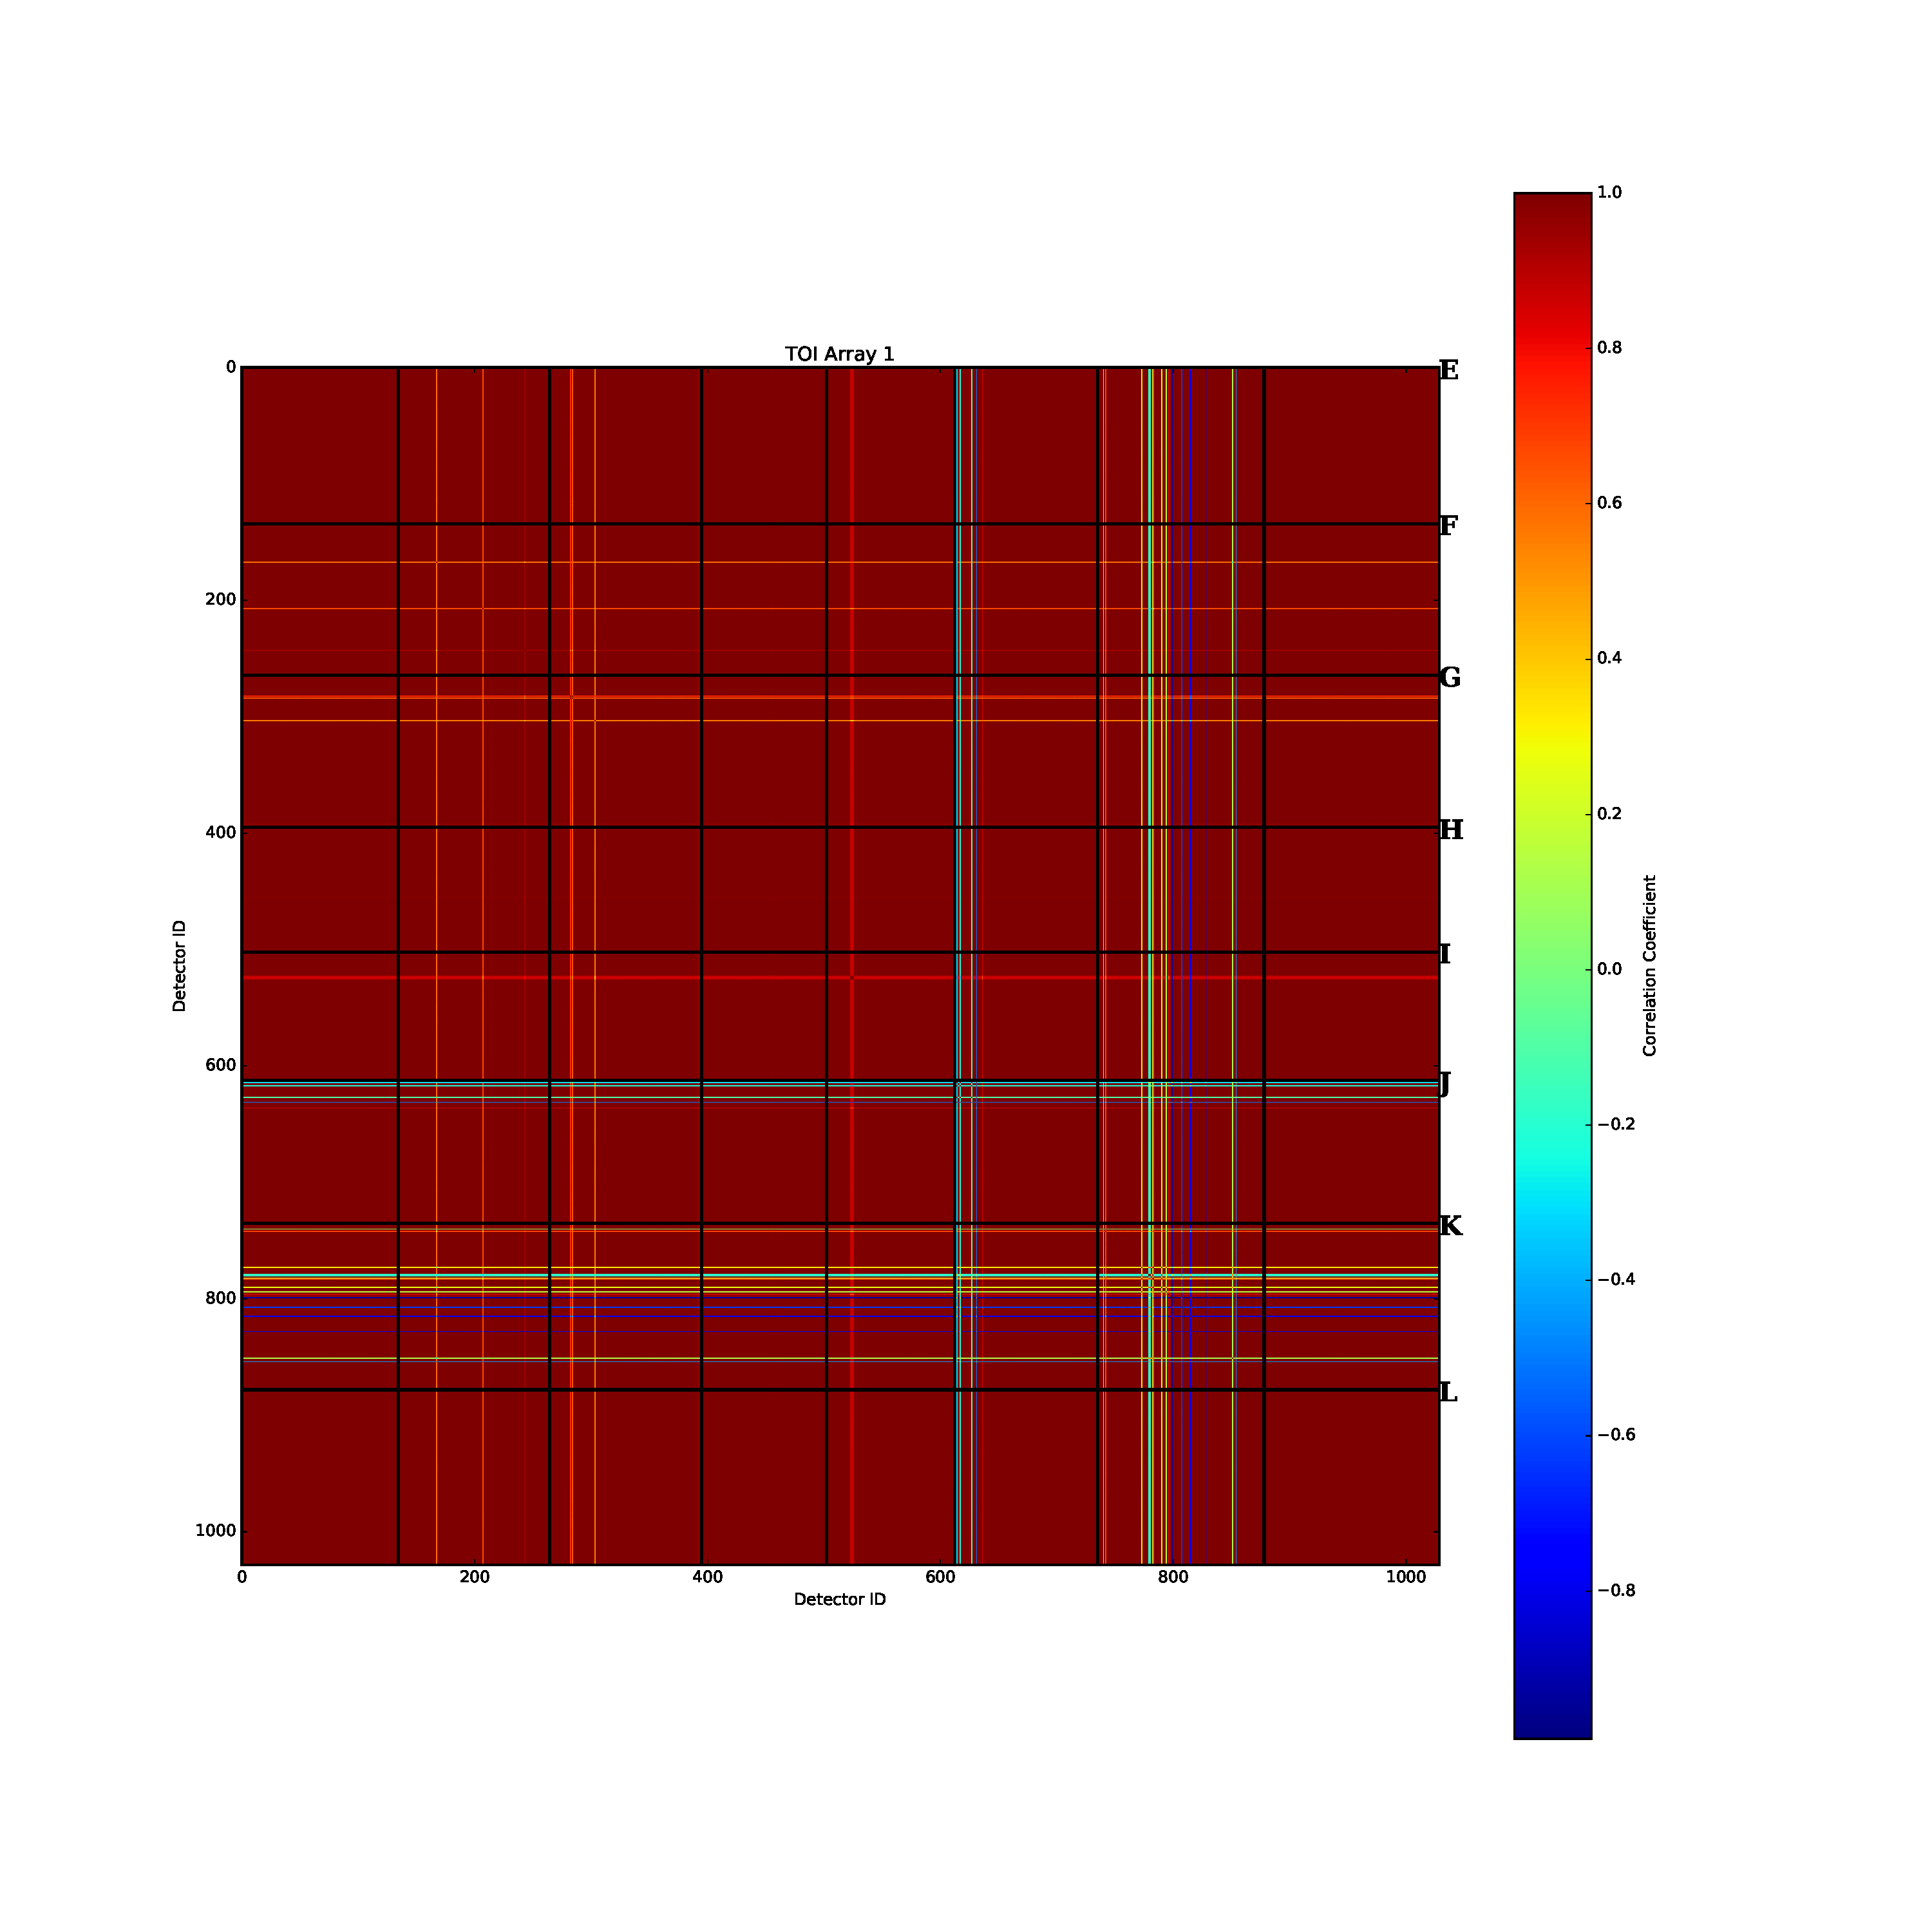
\includegraphics[width=0.3\textwidth]{Figures/DarkTests/corrmat_TOI_array_1_20160313s87.pdf}
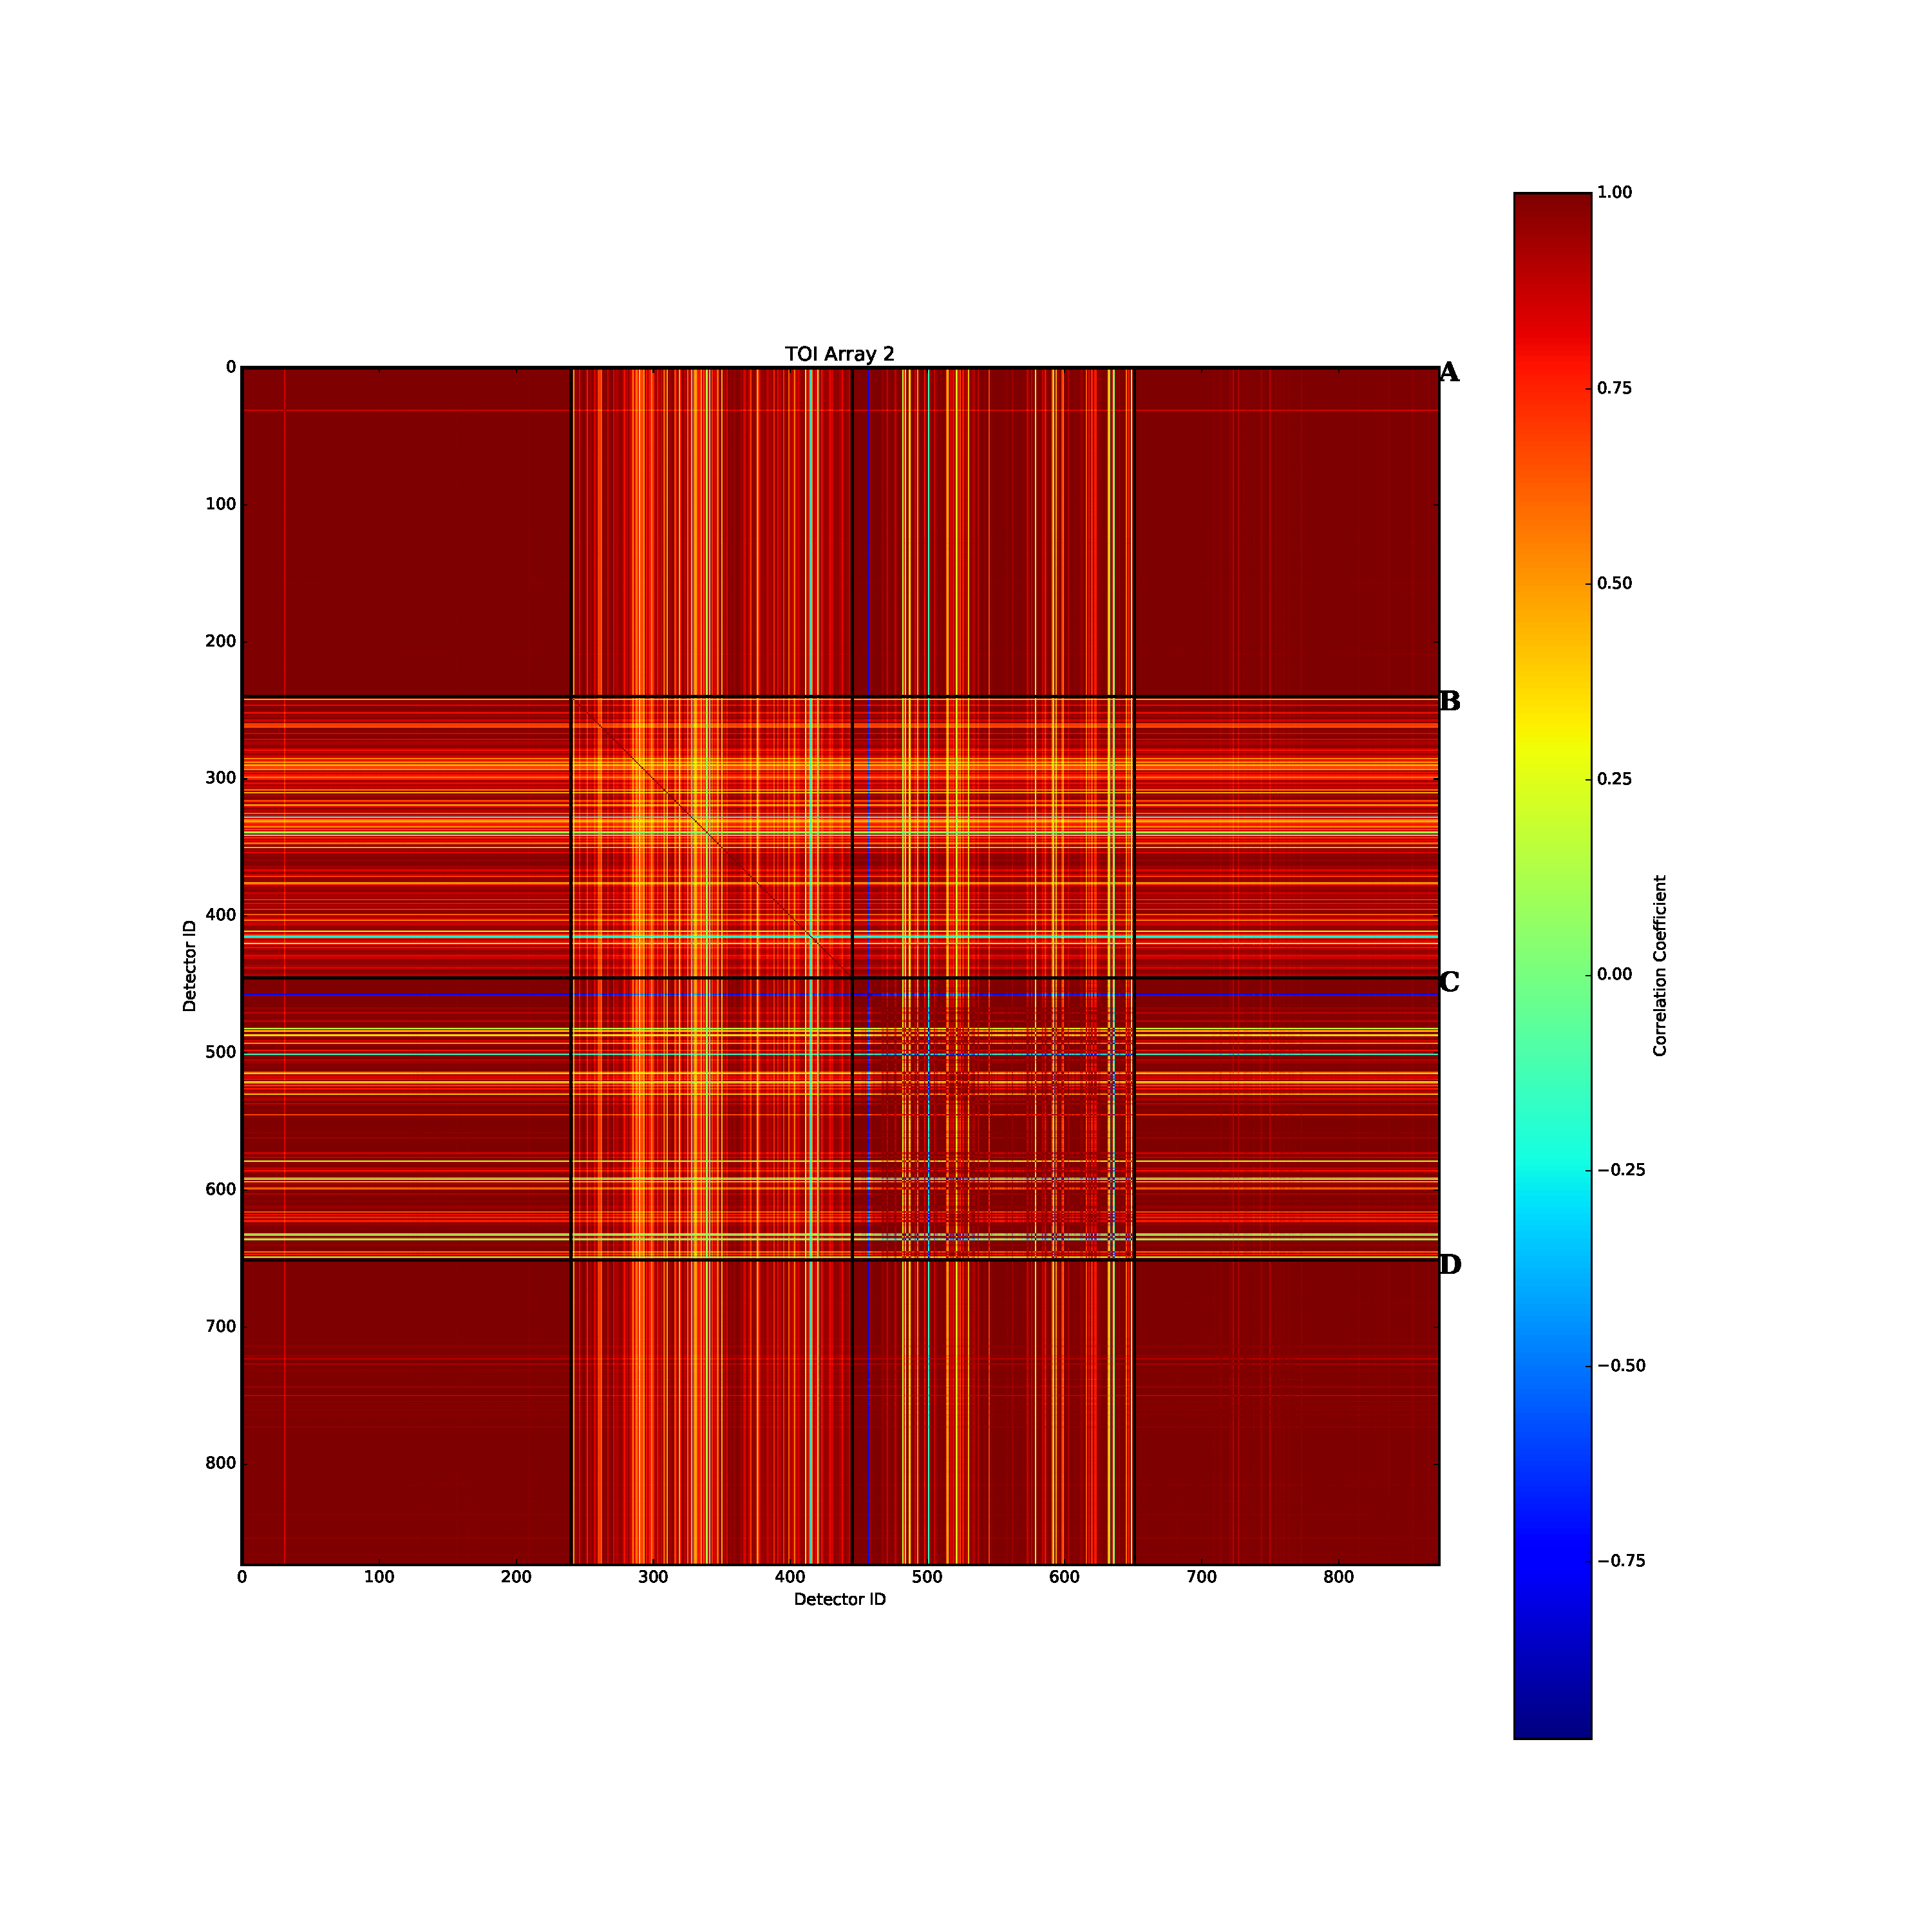
\includegraphics[width=0.3\textwidth]{Figures/DarkTests/corrmat_TOI_array_2_20160313s87.pdf}
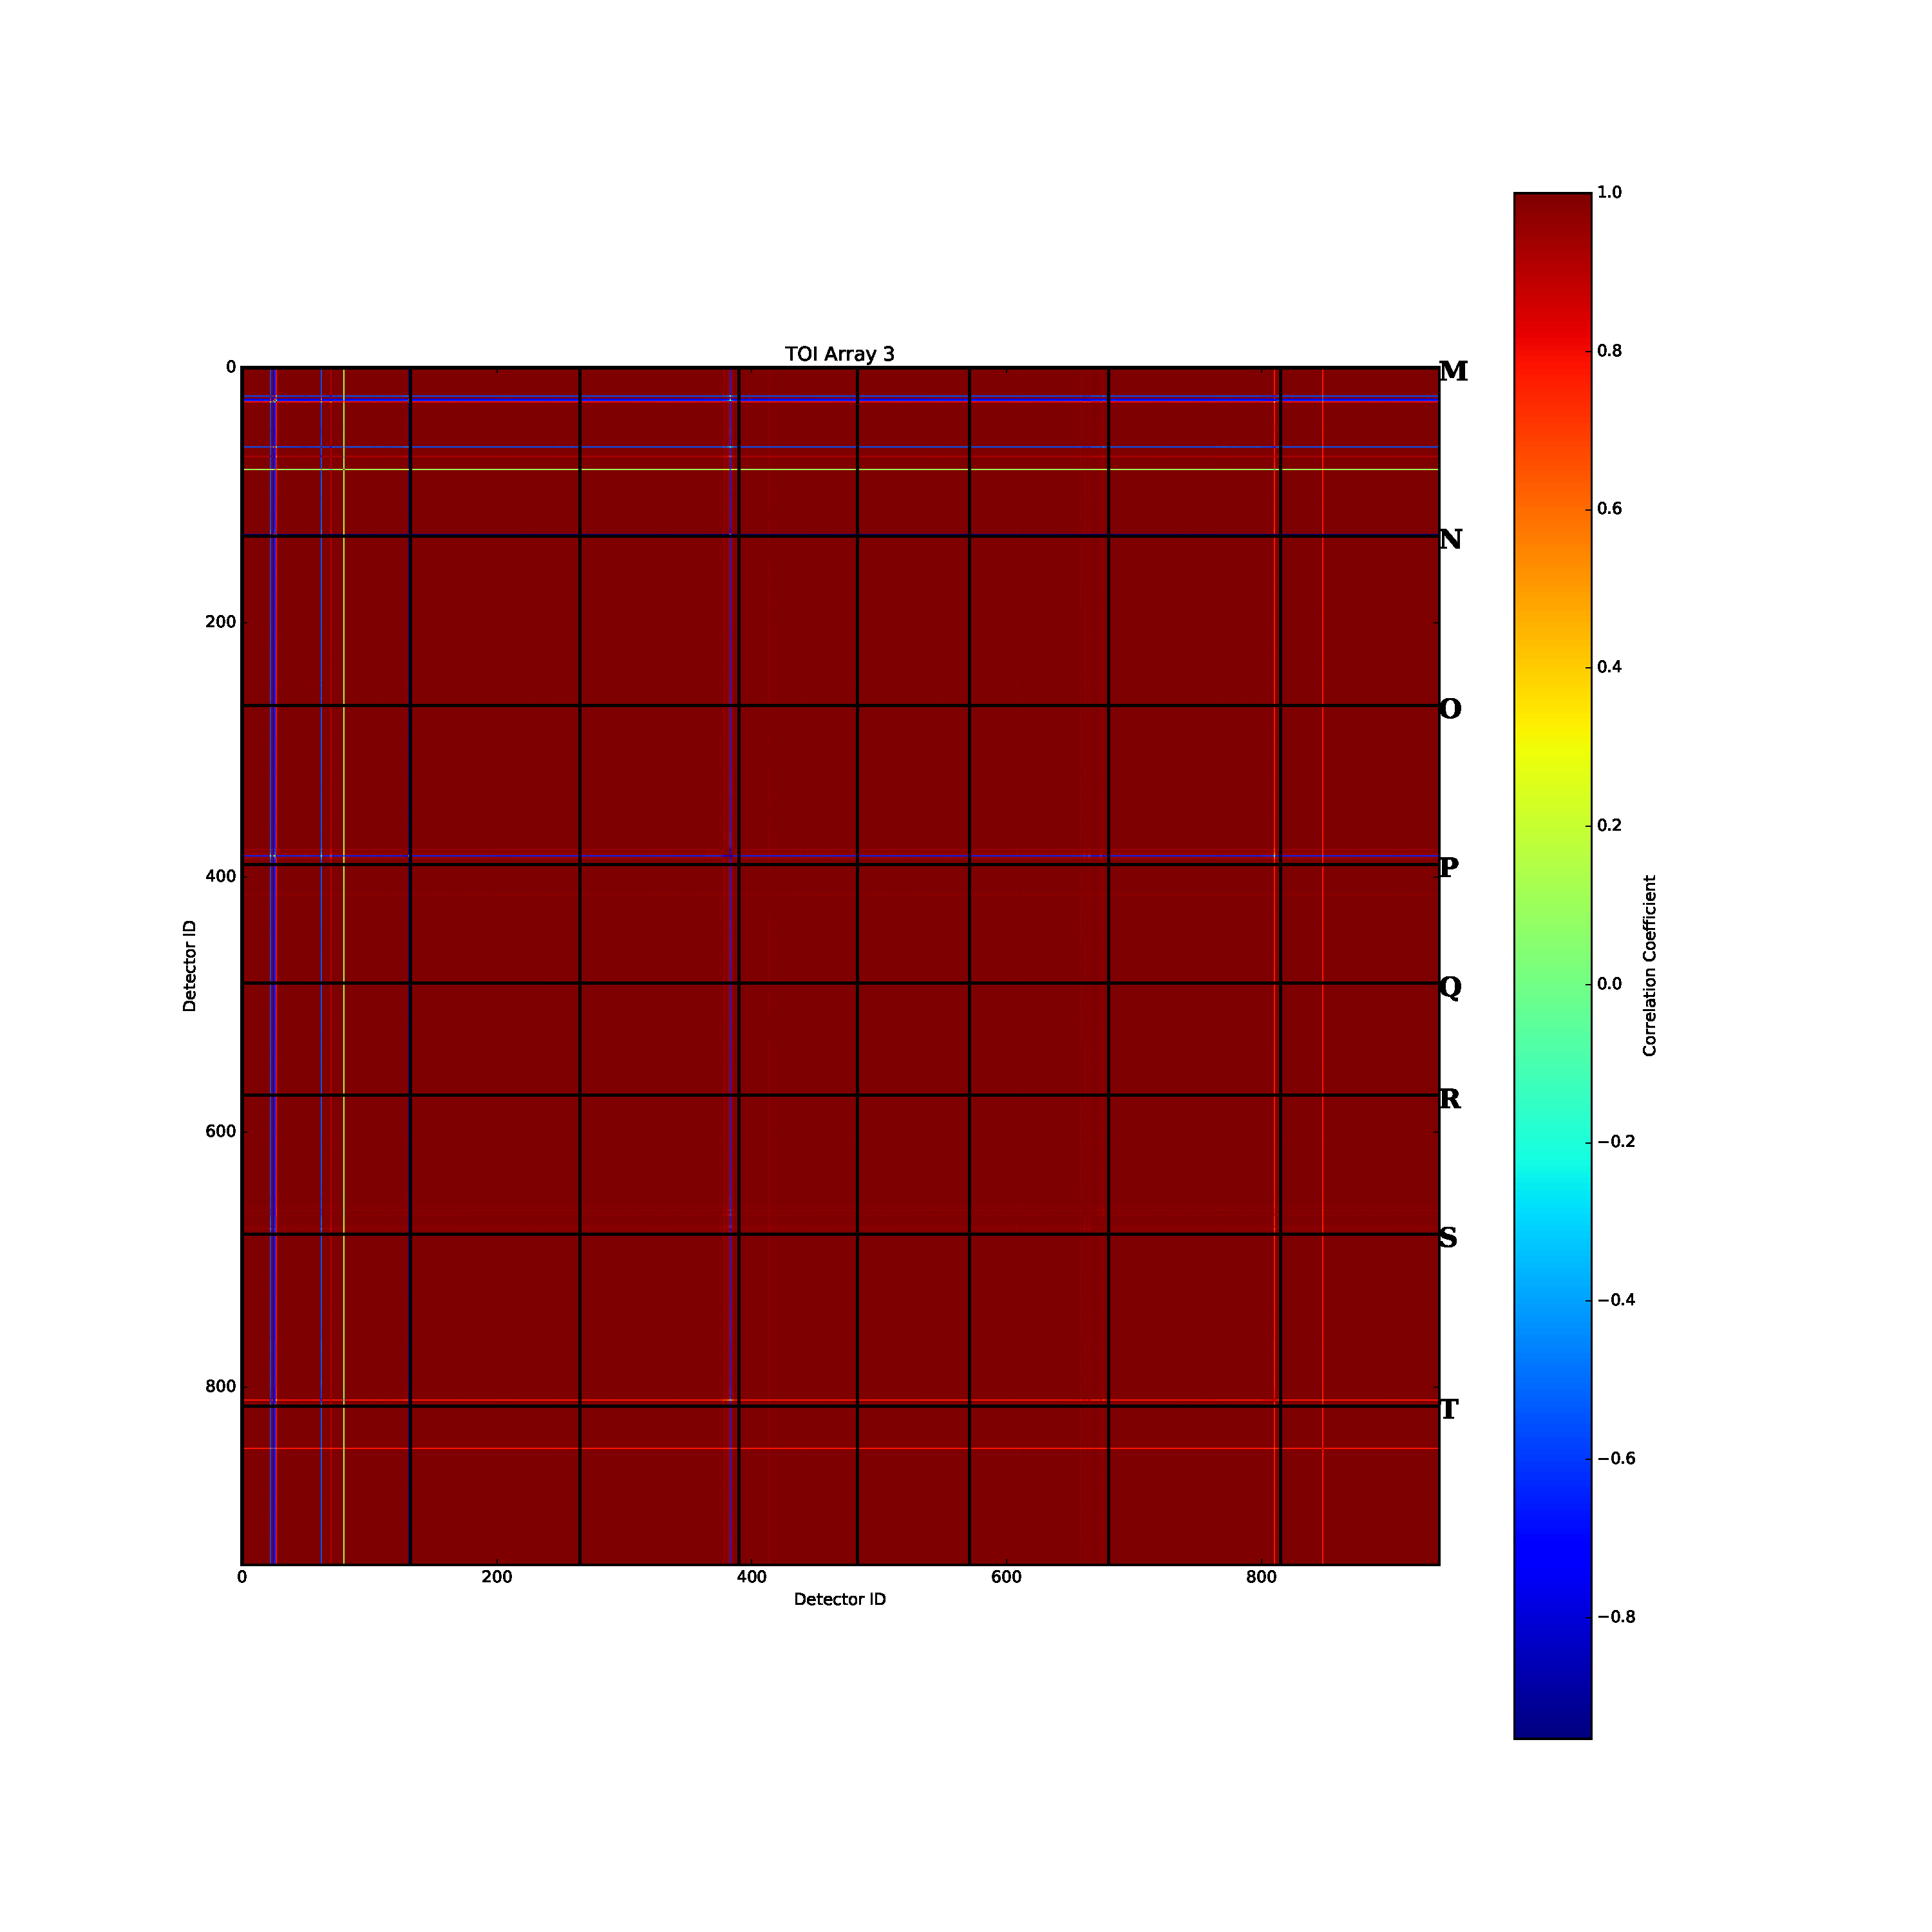
\includegraphics[width=0.3\textwidth]{Figures/DarkTests/corrmat_TOI_array_3_20160313s87.pdf}
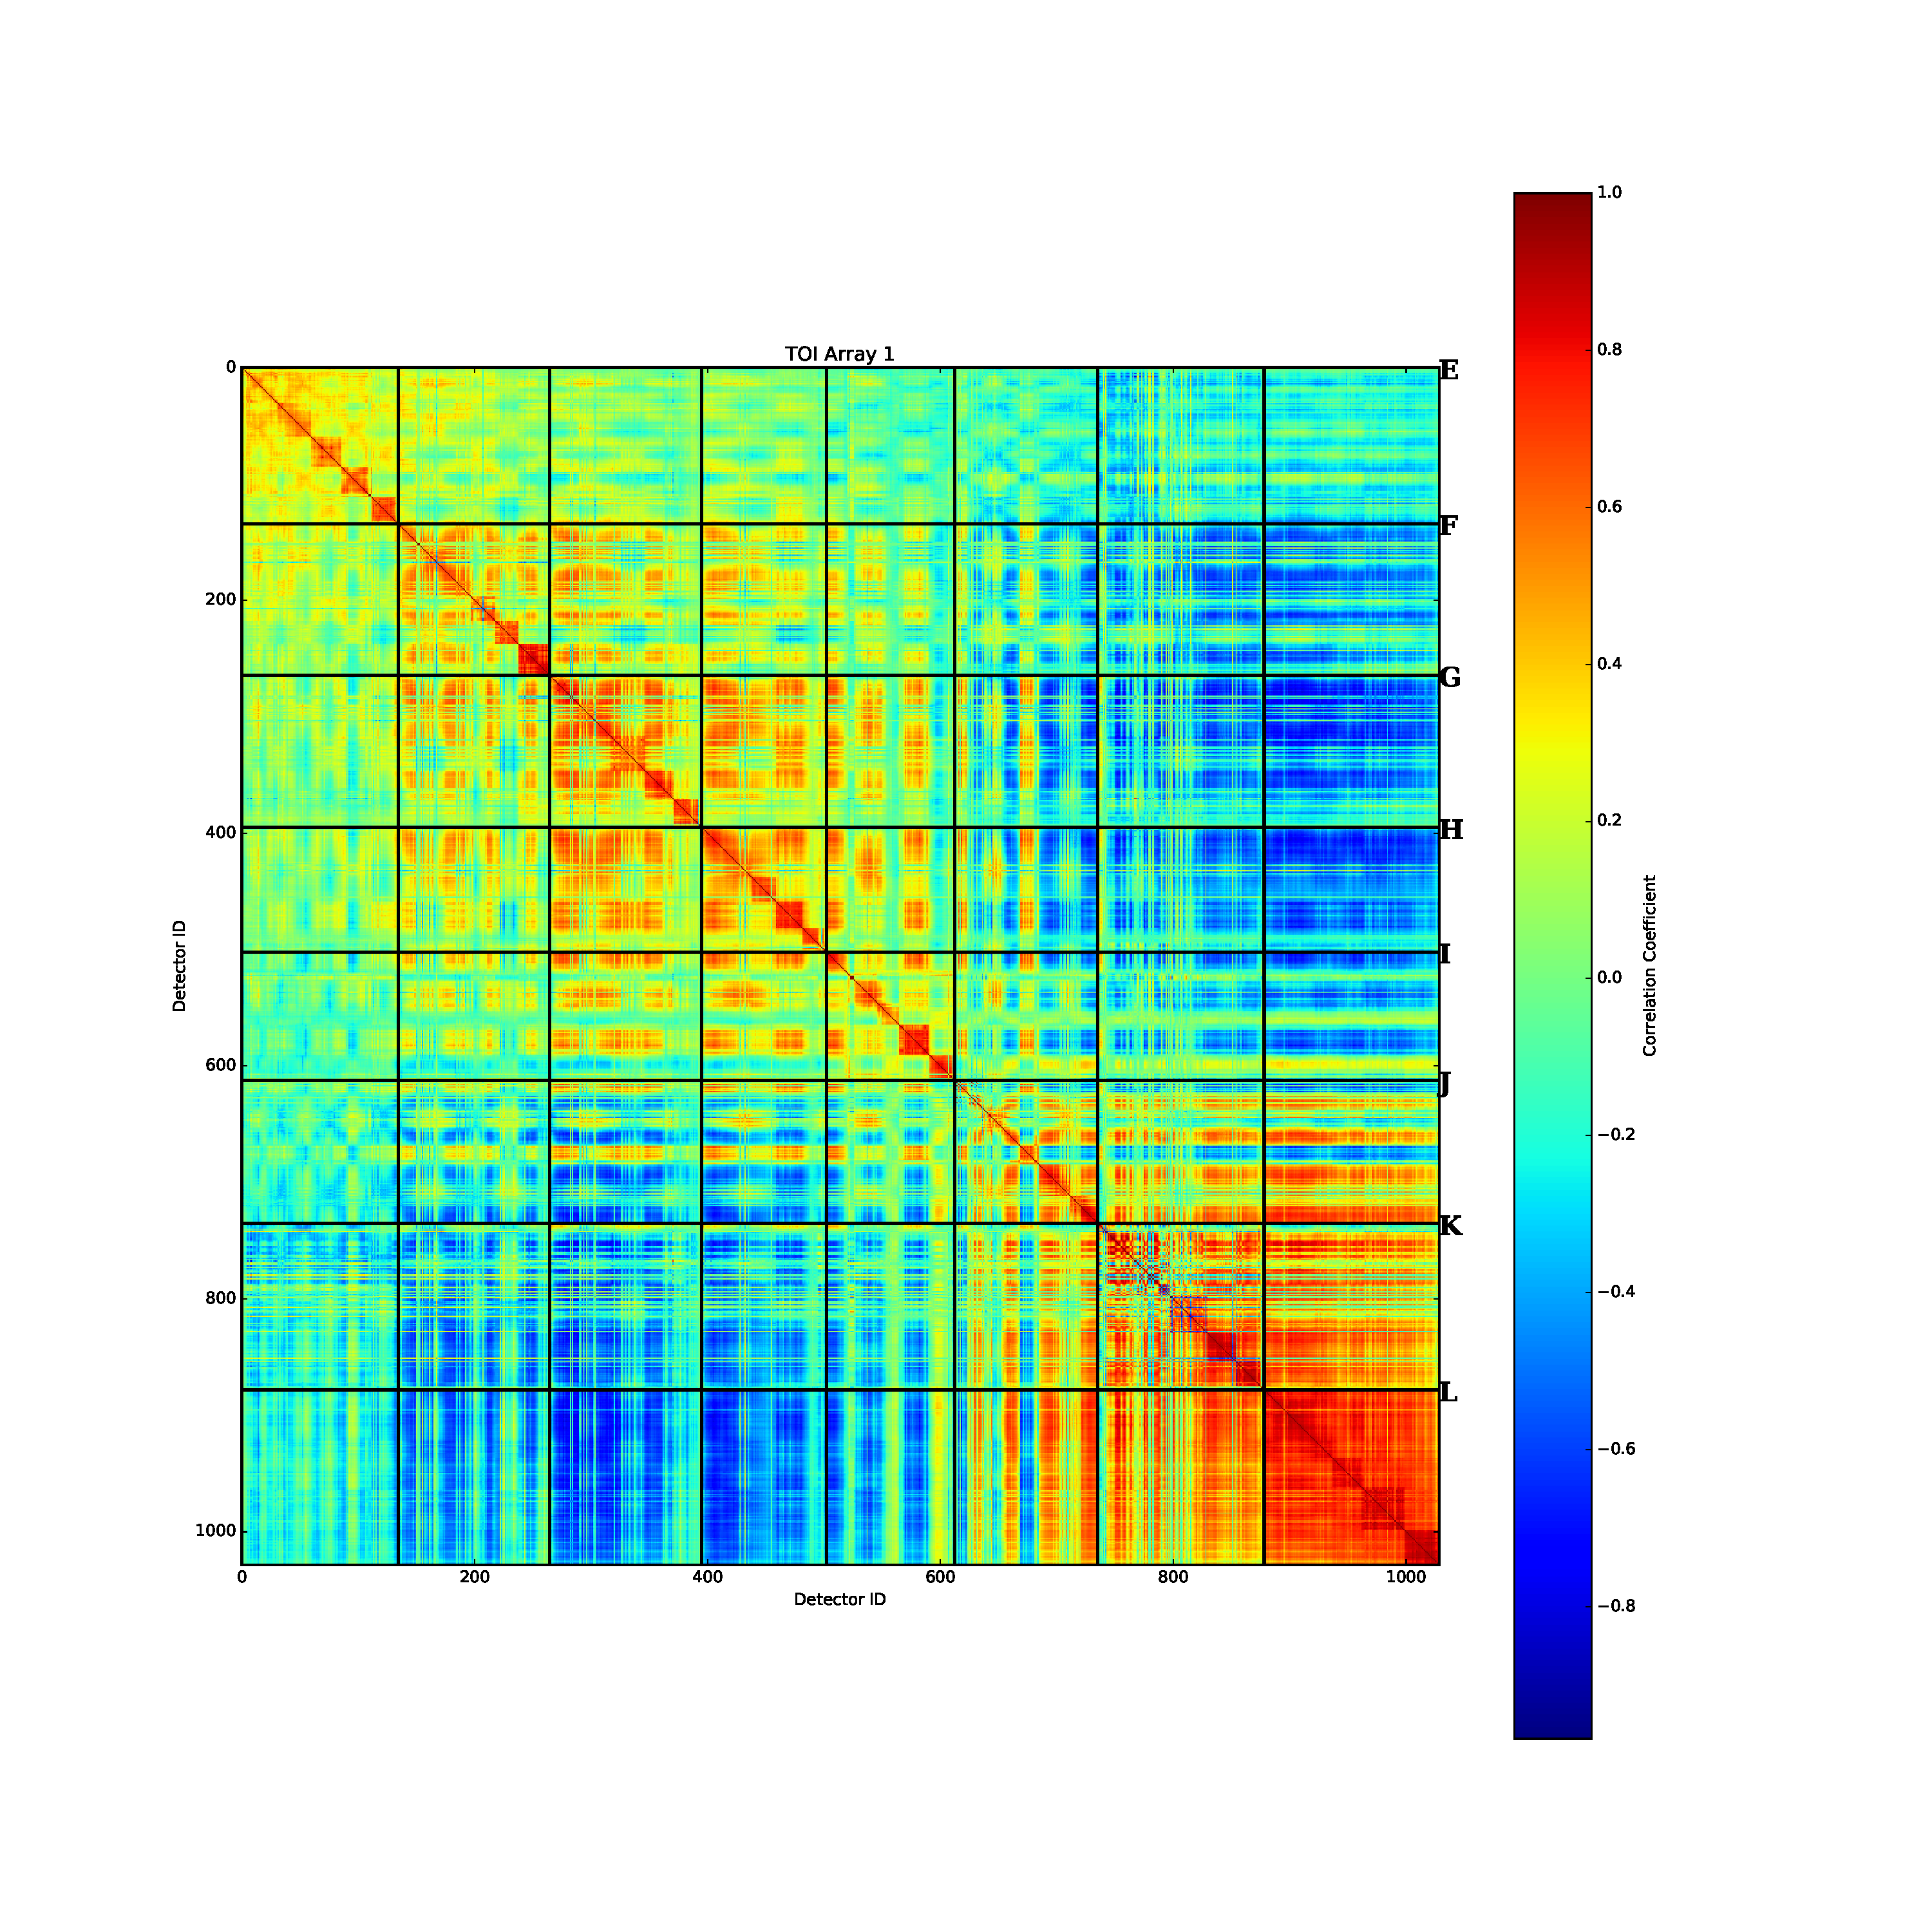
\includegraphics[width=0.3\textwidth]{Figures/DarkTests/corrmat_TOI_CM_array_1_20160313s87.pdf}
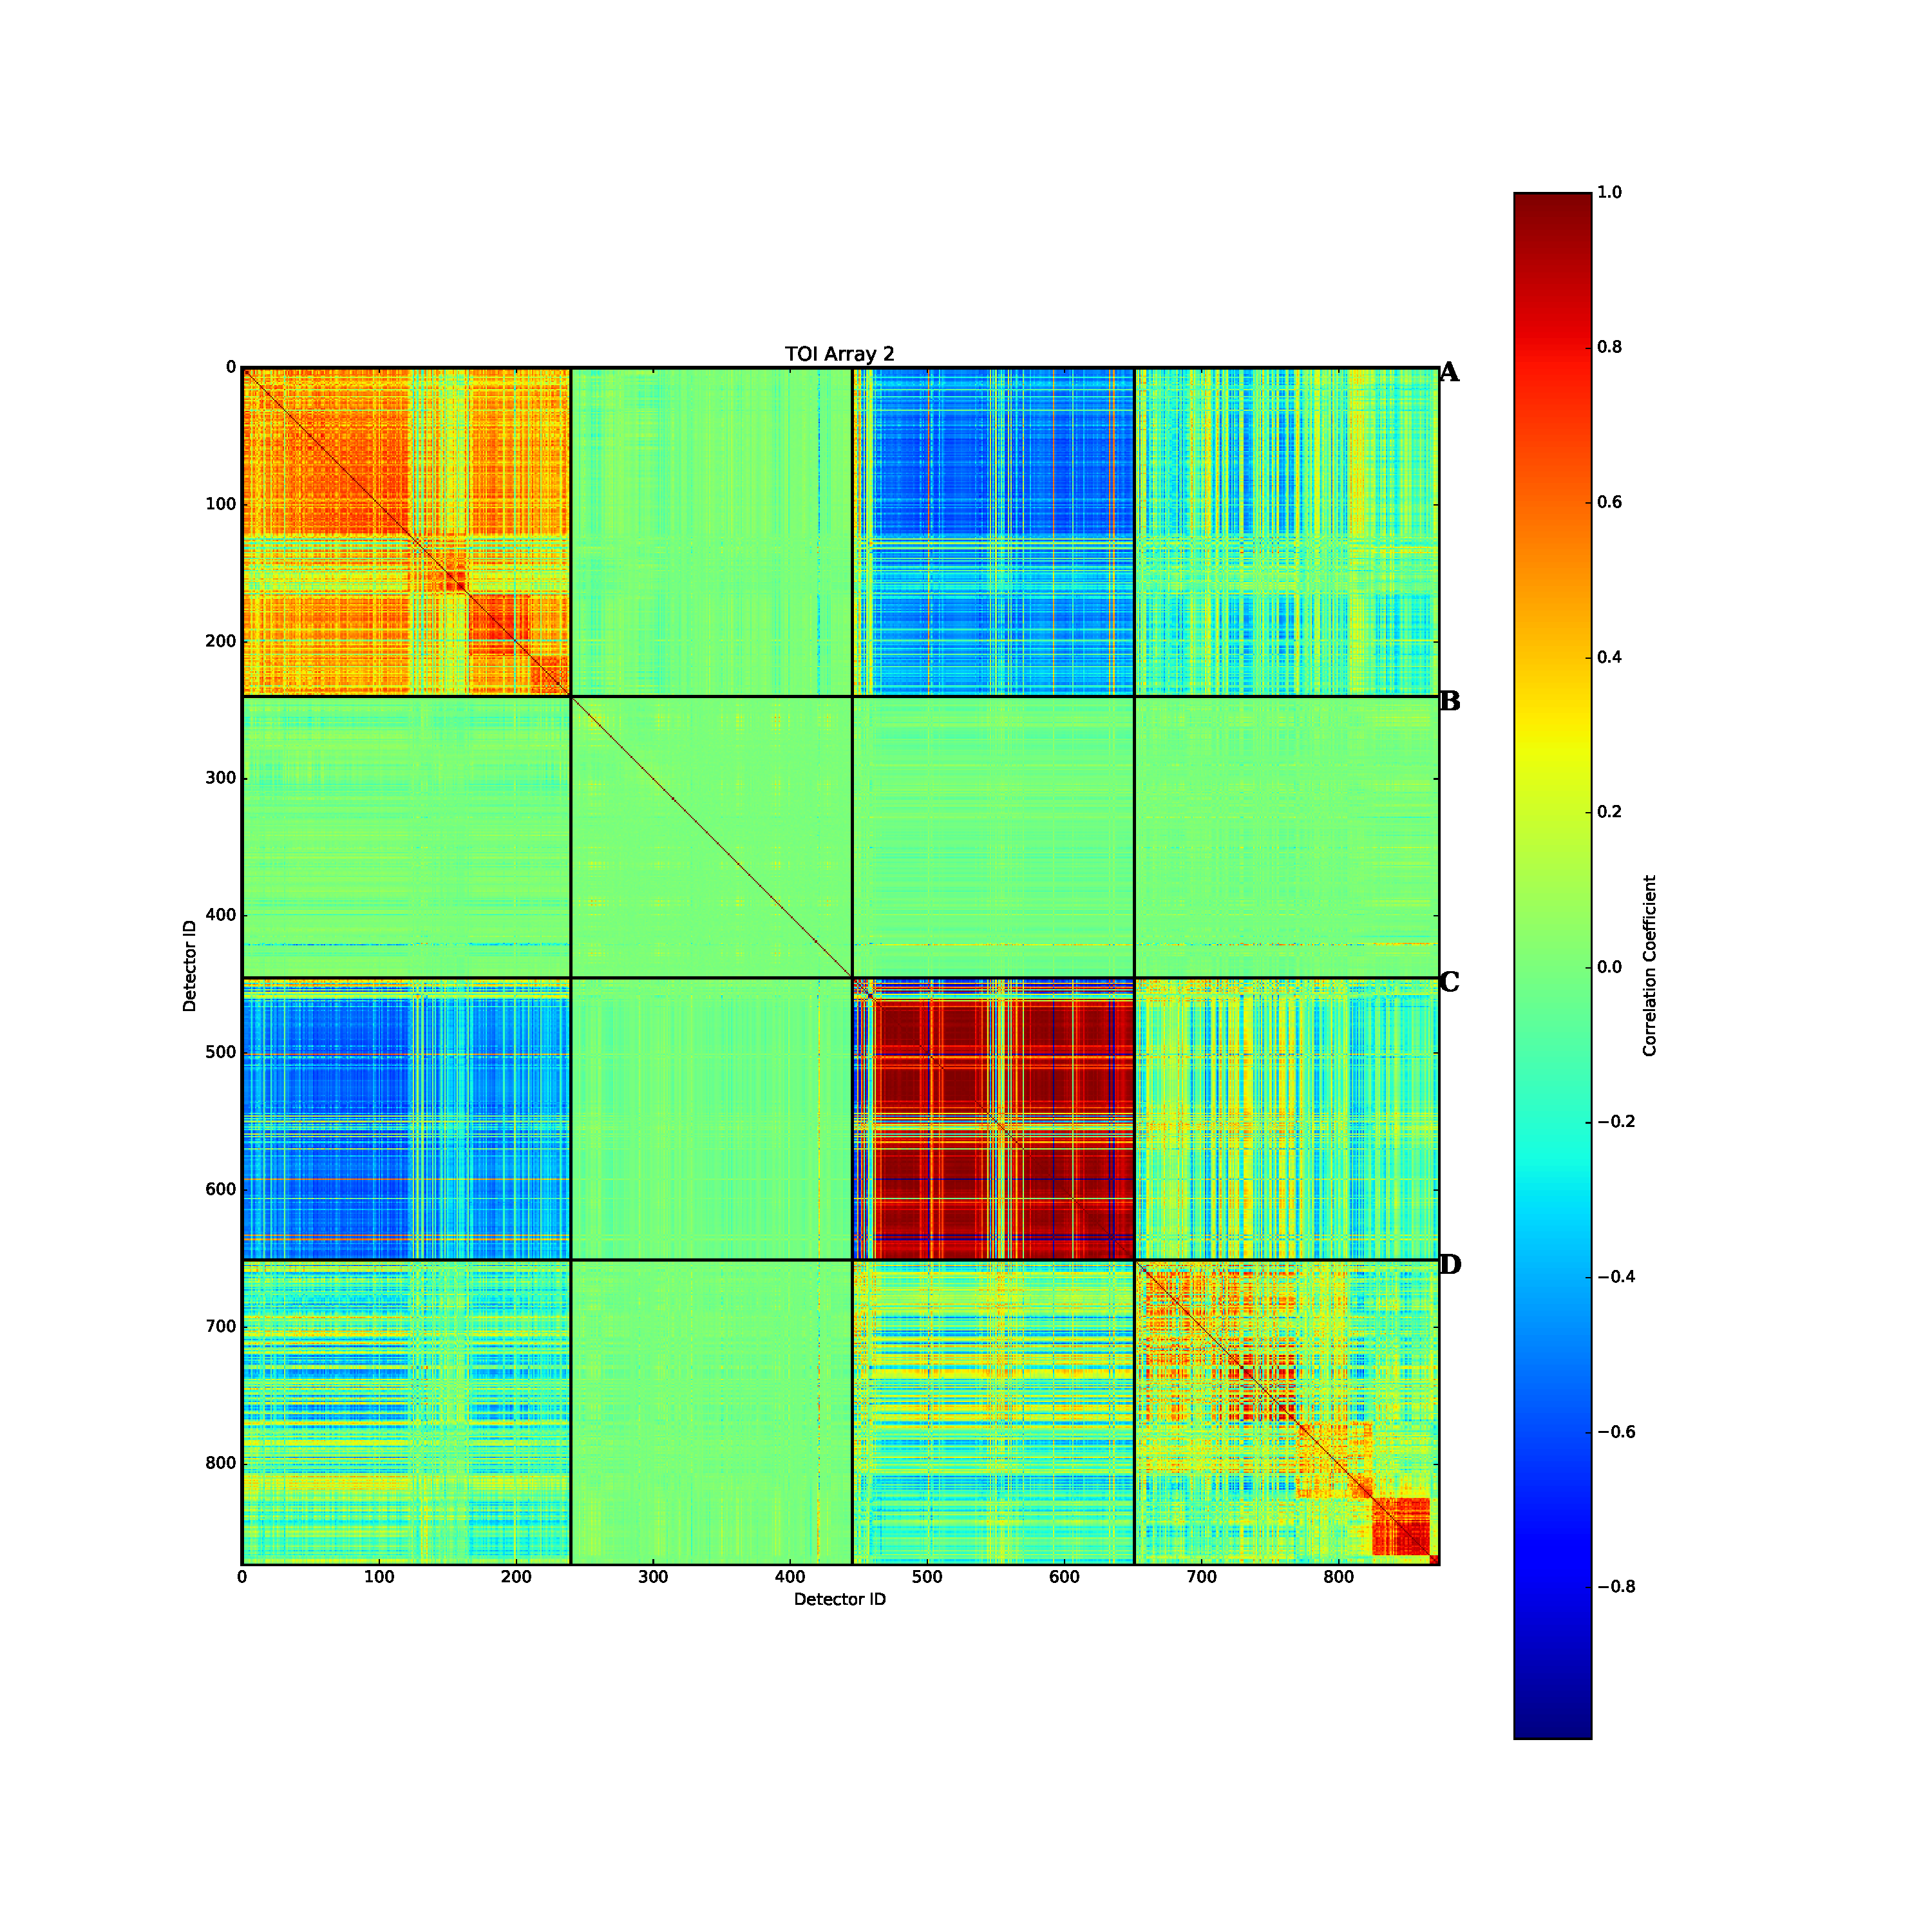
\includegraphics[width=0.3\textwidth]{Figures/DarkTests/corrmat_TOI_CM_array_2_20160313s87.pdf}
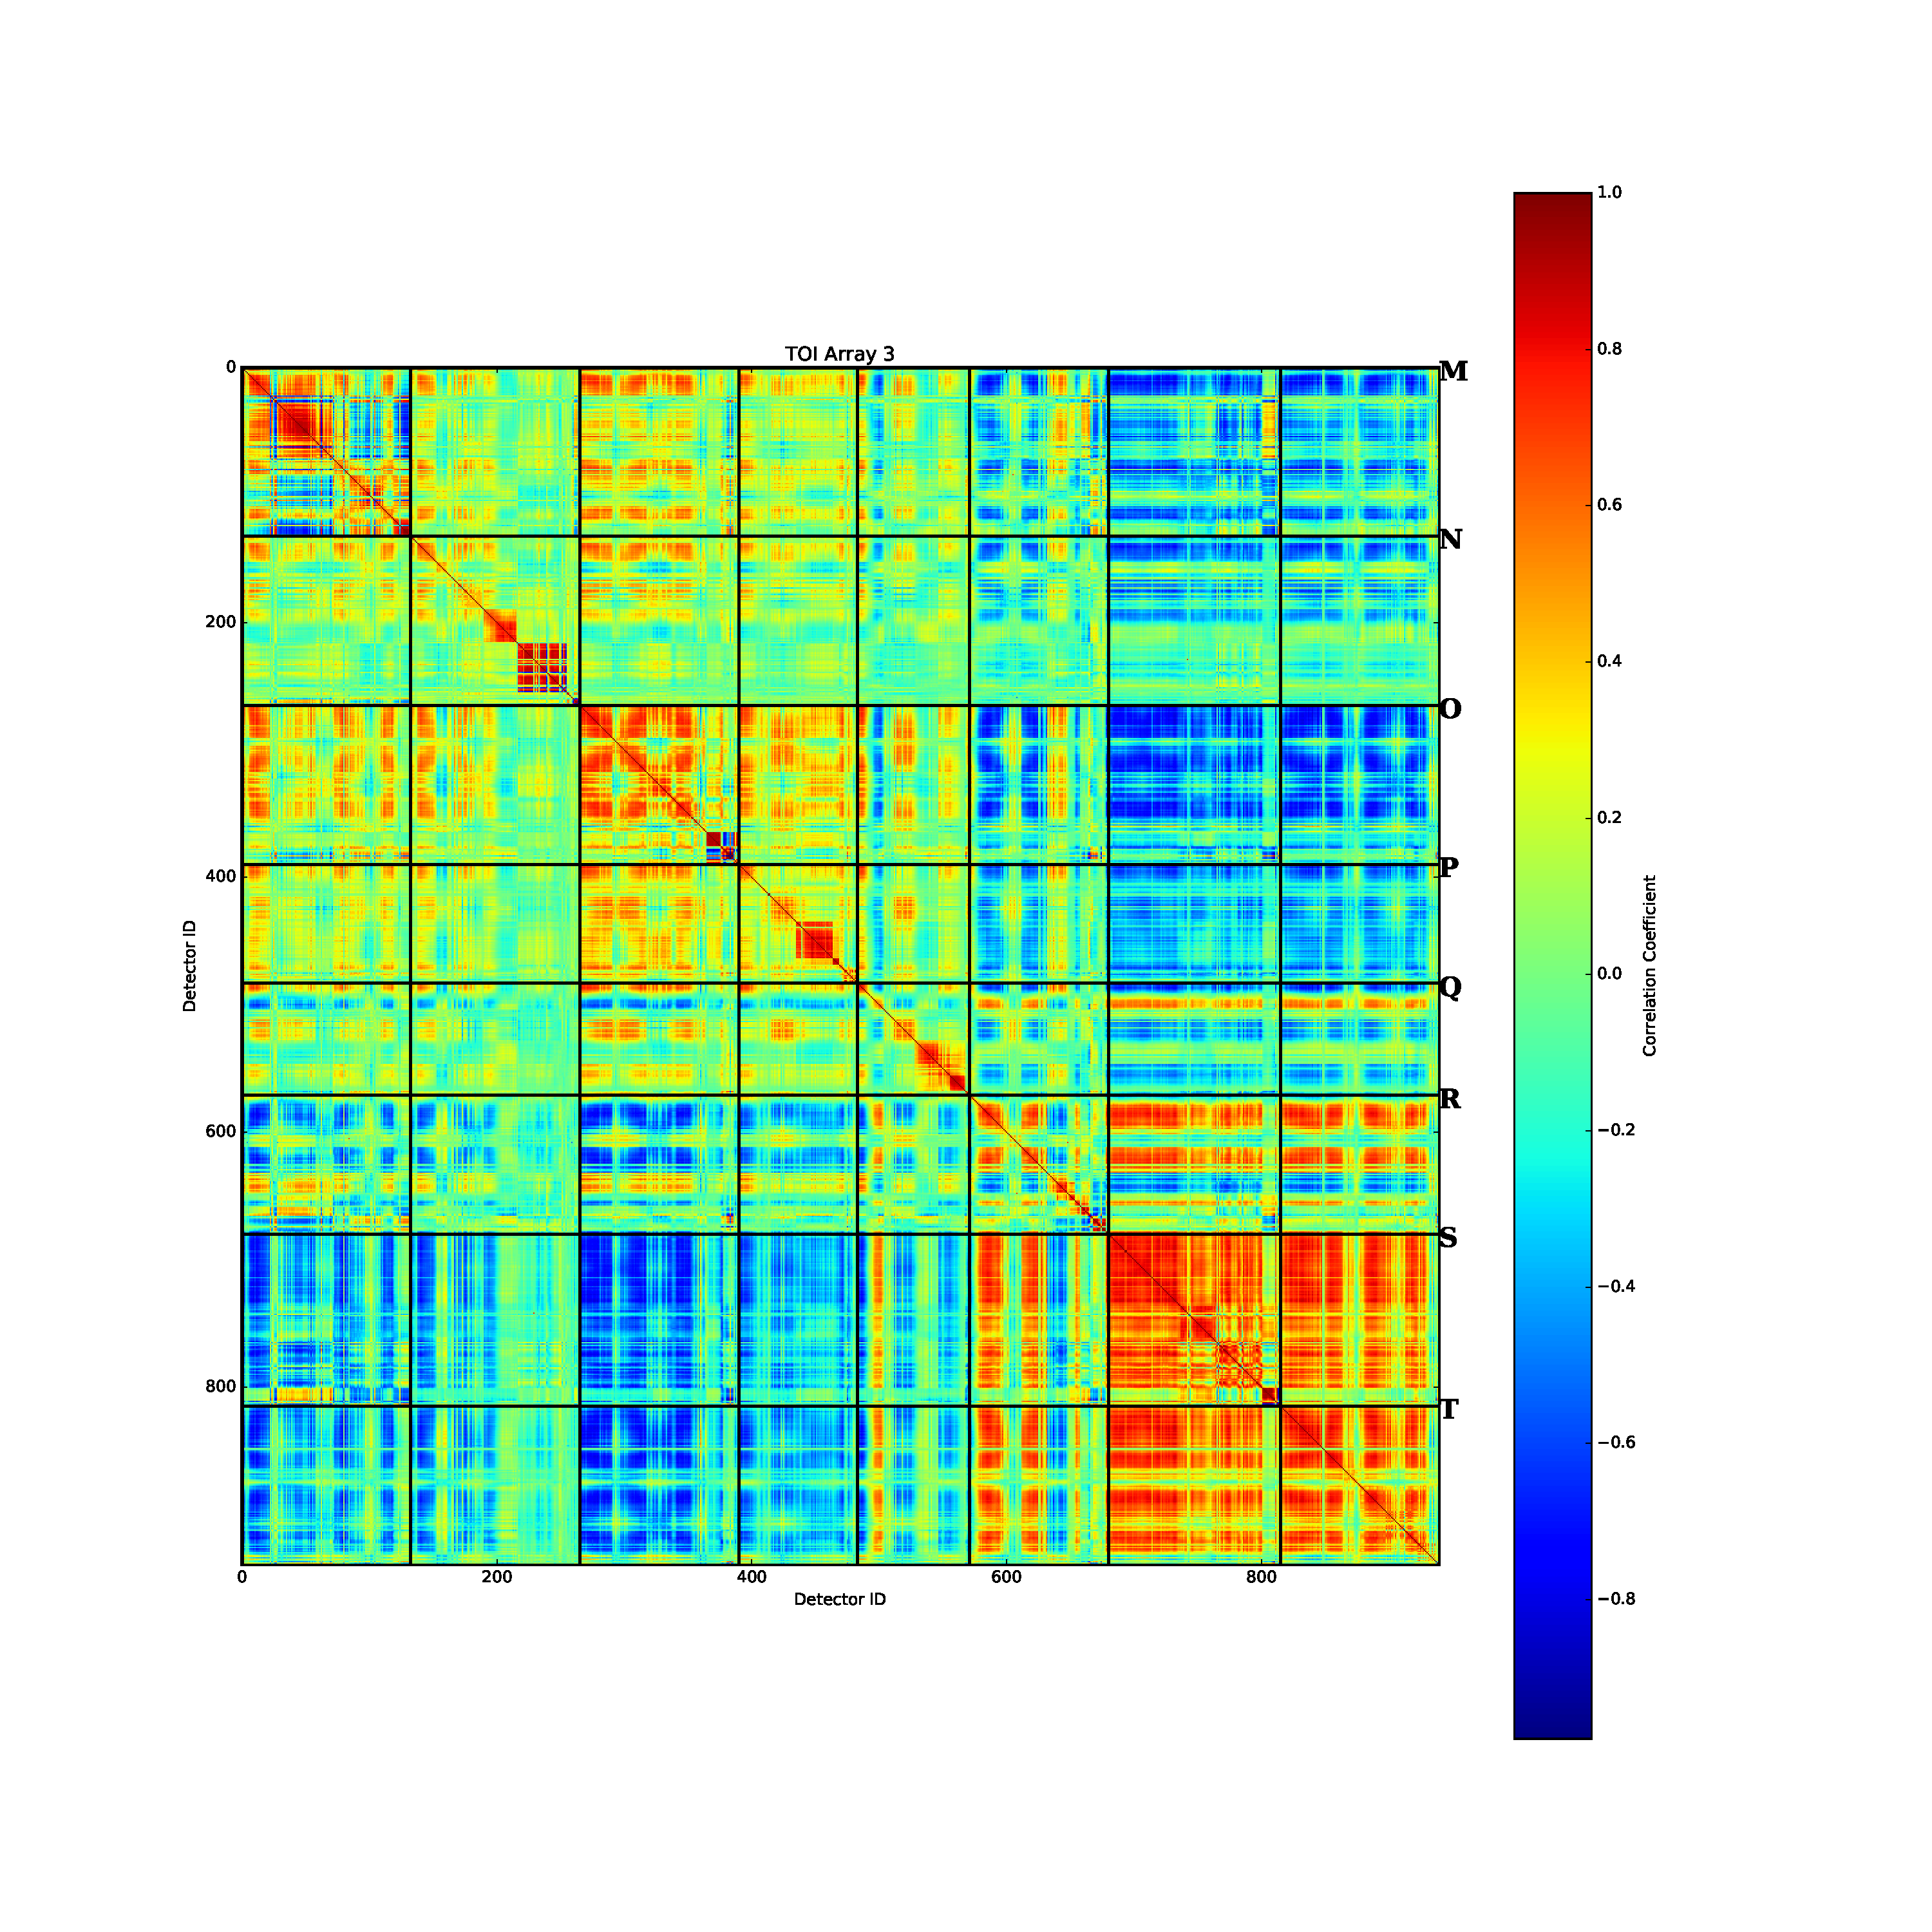
\includegraphics[width=0.3\textwidth]{Figures/DarkTests/corrmat_TOI_CM_array_3_20160313s87.pdf}
\includegraphics[width=0.3\textwidth]{Figures/DarkTests/corrmat_TOI_PCA_array_1_20160313s87.pdf}
\includegraphics[width=0.3\textwidth]{Figures/DarkTests/corrmat_TOI_PCA_array_2_20160313s87.pdf}
\includegraphics[width=0.3\textwidth]{Figures/DarkTests/corrmat_TOI_PCA_array_3_20160313s87.pdf}
\includegraphics[width=0.3\textwidth]{Figures/DarkTests/corrmat_TOI_BC_array_1_20160313s87.pdf}
\includegraphics[width=0.3\textwidth]{Figures/DarkTests/corrmat_TOI_BC_array_2_20160313s87.pdf}
\includegraphics[width=0.3\textwidth]{Figures/DarkTests/corrmat_TOI_BC_array_3_20160313s87.pdf}
\end{center}
\caption{From left to right correlation matrices for the three NIKA2 arrays (A1, A2, and A3) for scan 20160313s87. From top to bottom we present the correlation of the raw data, after CM, PCA and BC decorrelations. \label{corrs87}}
\end{figure}


\subsection{RMS of the noise}

We present in Figure~\ref{rms299} the rms, in Hz, of the raw (dark blue) and decorrelated (CM, blue; PCA, red; and BC, cyan),data for the N2R7 dark test scan 21612101s299. We also show for comparison the rms of the data by extrapolating the median high frequency noise (PS, violet).
For the three arrays we observe that decorrelation reduces significantly the rms noise. The most efficient method is PCA as one would expect from previous results in the noise correlation matrix. \\

For each array the detectors are ordered by electronic box (separated by vertical black lines in the figure) and within each electronic box by increasing resonant frequency. We observe that median high frequency noise increases with increasing resonant frequency. A similar effect is observed for the PCA and BC rms noise but for some pathological detectors or electronic boxes. While in A2 the rms noise increases monotoneously with resonant frequency in arrays A1 and A3 we observe also observe fine structure within eash electronic box. For array A2, electronic box A, shows significantly larger raw rms. For array A1 box K seems to have a larger number of anomalous detectors than the other boxes. In array A3 all boxes seem to be equivalent to first order. Both in A1 and A3 we find complex structure within each box, which are not present in A2. \\

Similar results are found for scan 20161213s72 as shown in Figure~\ref{rms72}. However, we stress that the atmospheric emission shows significant contribution at high frequency (see PS) that is significantly reduced after decorrelation. \\

We have also computed the noise rms for the scans of N2R4 20160504s97 and 20160313s87. For arrays A1 and A3 the results are very similar to those for the N2R7 scans. However, we clearly observe that A2 is significantly worse in terms of misbehaving pixels.


%------------------------------------------------
\begin{figure}[ht] % Inline image example
\begin{center}
\includegraphics[scale=0.26]{Figures/DarkTests/rms_TOI_array_1_20161211s299.pdf} 
\includegraphics[scale=0.26]{Figures/DarkTests/rms_TOI_array_2_20161211s299.pdf} 
\includegraphics[scale=0.26]{Figures/DarkTests/rms_TOI_array_3_20161211s299.pdf} 
\end{center}
\caption{RMS noise for arrays 1,2,and 3 (top to bottom) for scan 20161211s299. The rms is computed for the raw data, and for the three decorrelation methods, CM. PCA and BC. The rms value for the level of white is also computed from the raw data power spectrum (PS). \label{rms299}}
\end{figure}


\begin{figure}[ht] % Inline image example
\begin{center}
\includegraphics[scale=0.26]{Figures/DarkTests/rms_TOI_array_1_20161213s72.pdf} 
\includegraphics[scale=0.26]{Figures/DarkTests/rms_TOI_array_2_20161213s72.pdf} 
\includegraphics[scale=0.26]{Figures/DarkTests/rms_TOI_array_3_20161213s72.pdf} 
\end{center}
\caption{Same as Figure~\ref{rms299} but for scan 20161213s72. \label{rms72}}
\end{figure}

\begin{figure}[ht] % Inline image example
\begin{center}
\includegraphics[scale=0.26]{Figures/DarkTests/rms_TOI_array_1_20160504s97.pdf} 
\includegraphics[scale=0.26]{Figures/DarkTests/rms_TOI_array_2_20160504s97.pdf} 
\includegraphics[scale=0.26]{Figures/DarkTests/rms_TOI_array_3_20160504s97.pdf} 
\end{center}
\caption{Same as Figure~\ref{rms299} but for scan 20160504s97. \label{rms97}}
\end{figure}



\begin{figure}[ht] % Inline image example
\begin{center}
\includegraphics[scale=0.26]{Figures/DarkTests/rms_TOI_array_1_20160313s87.pdf} 
\includegraphics[scale=0.26]{Figures/DarkTests/rms_TOI_array_2_20160313s87.pdf} 
\includegraphics[scale=0.26]{Figures/DarkTests/rms_TOI_array_3_20160313s87.pdf} 
\end{center}
\caption{Same as Figure~\ref{rms299} but for scan 20160313s87. \label{rms87}}
\end{figure}



\subsection{Discussion}

Using dark test measurements we have identified several noise components that require using complex decorrelation methods. Event in the case of multiple template decorrelation we find residual correlation between detectors that seems to be related to electronic subbands. Similar results are found when analyzing faint source scans. We find significant differences between N2R4 and N2R7 scans. \\

After decorralation using multiple template procedures we reduce significantly the rms of the noise. In the case of dark test it becomes of the level of the high frequency noise. For faint source scans we also diminish the high frequency noise, which is probably dominated by atmospheric emission. We find significant differences between the noise levels in A1 and A3, which might be explained by gain differences (to be verified). For some electronic boxes in A2 the rms noise is significantly larger than for the others. For the three arrays we find increasing noise with increasing resonant frequency withing each electronic box.This is probably related to the difference of gains between subbands in the electronics. Furthermore, we find in A1 and A3 extra low frequency structures in the rms which are not identified yet.

%------------------------------------------
\section{Summary of performance}

%----------------------------------------------------------------------------------------
%	BIBLIOGRAPHY
%----------------------------------------------------------------------------------------

\bibliographystyle{unsrt}

\bibliography{sample}

%----------------------------------------------------------------------------------------

\end{document}
